%% This is file `skeleton.tex',
%% generated with the docstrip utility.
%%
%% The original source files were:
%%
%% nuthesis.dtx  (with options: `skeleton')
%% For common degrees, you can use the class options:
%% phd, edd, ms, ma
%% phd is the default


\documentclass[print]{nuthesis}
\usepackage{mathptmx}
\usepackage{graphicx}
\graphicspath{ {nuthesis/images/} }
\usepackage{times}
\usepackage{epstopdf}
\usepackage{amsmath}
%\usepackage{program}
%\usepackage{amssymb}
%\usepackage{algorithmic}
\usepackage{algorithm}
\usepackage{algpseudocode}

%%% My packages

\usepackage[english]{babel}
\usepackage[T1]{fontenc}
\usepackage{latexsym}
\usepackage{float}
\usepackage{amsthm}
\usepackage{amsfonts}
\usepackage{epsfig}
%\usepackage{subfigure} % subfiguras
\usepackage{hyperref}
\usepackage{amssymb}
%\usepackage[pdftex]{color,graphicx}
%\usepackage{epstopdf}
\usepackage{color} %Paquete para escribir letras en color
%\usepackage[pdftex]{hyperref}
%\usepackage[dvips]{graphicx}
%\usepackage{setspace}
%\singlespacing
%\usepackage{fancyhdr}
\usepackage[hang]{footmisc}
\usepackage[font=small,labelfont=bf]{caption}
%\usepackage{biblatex}
%\usepackage{cite}
%\usepackage[noadjust]{cite}
\usepackage{pifont}
%\usepackage{amssymb}
\usepackage{multirow}

%\usepackage{titlesec}
\usepackage{xspace}

\usepackage{lmodern}
\usepackage{cite}
\usepackage{lineno}
\usepackage{arydshln} %for dashed lines
\usepackage{slashed}
\usepackage{bm}
\usepackage[normalem]{ulem}




\newcommand{\tHq}{\ensuremath{tHq}\xspace}
\newcommand{\tHW}{\ensuremath{tHW}}
\newcommand{\tH}{\ensuremath{tH}}
\newcommand{\ttH}{\ensuremath{t\bar{t}H}\xspace}
\newcommand{\ttZ}{\ensuremath{t\bar{t}Z}}
\newcommand{\ttW}{\ensuremath{t\bar{t}W}}
\newcommand{\ttV}{\ensuremath{t\bar{t}\mathrm{V}}}
\newcommand{\WW}{\ensuremath{WW}\xspace}
\newcommand{\WZ}{\ensuremath{WZ}\xspace}
\newcommand{\ZZ}{\ensuremath{ZZ}\xspace}
\newcommand{\tautau}{\ensuremath{\tau\tau}\xspace}
\newcommand{\Zll}{\ensuremath{\mathrm{Z}\to\ell^+\ell^-}\xspace}
\newcommand{\Ztt}{\ensuremath{\mathrm{Z}\to\tau^+\tau^-}\xspace}
\newcommand{\reliso}{\ensuremath{I_\mathrm{rel}}\xspace}
\newcommand{\sip}{\ensuremath{S_\mathrm{IP3D}}\xspace}
\newcommand{\Pgth}{\ensuremath{\Pgt_{\rm h}}\xspace}
\newcommand{\ptRatio}{\ensuremath{\pt^\text{ratio}}\xspace}
\newcommand{\ptRel}{\ensuremath{\pt^\text{rel}}\xspace}
\newcommand{\relIso}{\ensuremath{I_\text{rel}}\xspace}
\newcommand{\miniIso}{\ensuremath{I_\text{mini}}\xspace}
\newcommand{\CV}{\ensuremath{\kappa_\text{V}}\xspace}
\newcommand{\Ct}{\ensuremath{\kappa_t}\xspace}
\newcommand{\ft}{\ensuremath{f_t}\xspace}
\newcommand{\mumu}{\ensuremath{\Pgm^\pm\Pgm^\pm}\xspace}
\newcommand{\emu}{\ensuremath{\Pe^\pm\Pgm^\pm}\xspace}
\newcommand{\ee}{\ensuremath{\Pe^\pm\Pe^\pm}\xspace}
\newcommand{\threel}{\ensuremath{\ell\ell\ell}\xspace}
\newcommand{\fbinv}{\ensuremath{fb^{-1}}\xspace}
\newcommand{\ttbar}{\ensuremath{t\bar{t}}\xspace}
\newcommand{\pt}{\ensuremath{p_T}\xspace}
\newcommand{\Et}{\ensuremath{E_T}\xspace}
\newcommand{\bjet}{\ensuremath{b}\xspace}
\newcommand{\ie}{i.e.\xspace}
\newcommand{\wpm}{\ensuremath{W^\pm}\xspace}
%\newcommand{\z0}{\ensuremath{z^0}\xspace}
\newcommand{\Lagr}{\mathcal{L}}
\newcommand{\beqn}{\begin{equation}}
\newcommand{\eeqn}{\end{equation}}
\newcommand{\bit}{\begin{itemize}}
\newcommand{\eit}{\end{itemize}}
\newcommand{\pp}{\ensuremath{pp}\xspace}
\newcommand{\etac}{\ensuremath{\eta}\xspace} %\etac=\eta coord
\newcommand{\phic}{\ensuremath{\phi}\xspace}
\newcommand{\dt}{\ensuremath{\mathcal{DT}}\xspace}
\newcommand{\ti}{\textit}

\setcounter{secnumdepth}{4}
%% \titleformat{\chapter}[display]
%%             {\normalfont%
%%               \LARGE % %change this size to your needs for the first line
%%               \bfseries}{\chaptertitlename\ \thechapter}{20pt}{%
%%               \LARGE %change this size to your needs for the second line
%%             }


\addto\captionsenglish{% Replace "english" with the language you use
  \renewcommand{\contentsname}%
    {Table of Contents}%
}

\begin{document}

\linenumbers

\renewcommand\bibname{References}
%% Start formatting the first few special pages
%% frontmatter is needed to set the page numbering correctly
\frontmatter

\title{Search for production of a Higgs boson and a single top quark in multilepton final states in \MakeLowercase{pp} collisions at $\sqrt{\MakeLowercase{s}}=13$ T\MakeLowercase{e}V.}
\author{Jose Andres Monroy Monta{\~n}ez}
\adviser{Kenneth Bloom and Aaron Dominguez}
\adviserAbstract{Kenneth Bloom and Aaron Dominguez}
\major{Physics and Astronomy}
\degreemonth{July}
\degreeyear{2018}

%% For most people the following can be changed with a class
%% option. To manually set these, just uncomment the following and
%% make the needed changes.
\doctype{Dissertation}
\degree{Doctor of Philosophy}
\degreeabbreviation{Ph.D.}
%%
%% Now that we know everything we need, we can generate the title page
%% itself.
%%
\maketitle
%%
%% You have a maximum of 350 words for your abstract, which includes
%% your title, name, etc.
%%
%% Required




\begin{abstract}
 \footnotesize
The exciting work in HEP includes not only the analysis of the data taken by the experiment but also the development of detection systems. In this thesis, the results of the search for the production of a Higgs-boson in association with a single top-quark (\tH) are presented; the focus is on leptonic signatures provided by the $H \to WW$, $H \to \tau\tau$, and $H \to ZZ$ decay modes. This process is of particular interest due to its sensitivity to the relative sign of the top-Higgs coupling and the vector bosons-Higgs coupling.

%% %This sensitivity has its origin in the fact that the process can proceed through two ways where the Higgs boson is emitted either by the exchanged W boson or by the top quark; the strong interference of the two leading order Feynman diagrams makes the production cross section of this process highly sensitive to the relative sign of the top-Higgs coupling modifier, \Ct, and the coupling modifier of vector bosons to the Higgs, \CV.

%% %In an scenario where \Ct/\CV=-1.0, known as the inverted top coupling scenario (ITC), the cross section is increased by a factor of ten with respect to the standard model (SM) scenario where \Ct/\CV=-1.   

%% The analysis exploits signatures with two same-sign leptons or three leptons in the final state, and uses the 2016 data sample collected with the CMS detector at the LHC at a center of mass energy of 13 TeV
%% %, which corresponds to an integrated luminosity of 35.9 \fbinv
%% . Multivariate techniques are used to discriminate the signal from the dominant backgrounds. The analysis yields a 95\% confidence level (C.L.) upper limit on the combined \tH + \ttH production cross section times branching ratio of 0.64 pb, with an expected limit of 0.32 pb, for a scenario with \Ct = −1.0 and \CV = 1.0.
%% %Developments in Monte Carlo simulation methods allow the study of different scenarios in the \Ct-\CV phase space, thus, it was possible to exclude
%% Values of \Ct outside the range of -1.25 to +1.60 are exclude at 95\% C.L., assuming \CV = 1.0.

%% Sensitivity to CP mixing in the Higgs sector was investigated by considering scenarios for different values of the mixing angle $\alpha_{CP}$. Upper limits on the combined \tH + \ttH production cross section times branching ratio of 0.6 pb is set for a scenario with $\alpha_{CP}=180^o$ which corresponds to the scenario with \Ct = −1.0 and \CV = 1.0.

%% On the hardware side, contributions to the construction of the CMS forward pixel detector (FPix), responsible for tracking with extreme accuracy the paths of particles emerging from the proton-proton collisions at CMS. FPix is a modular detector composed of 672 modules built using a semiautomatic pick-and-place robotic system which integrates optical tools, pattern recognition algorithms, and glue dispensing subsystems, to locate the constituent module parts on the work field and glue them together with a precision of ~10 um. Fully assembled modules were tested and characterized.
The analysis exploits signatures with two same-sign leptons or three leptons in the final state and uses the 2016 data sample collected with the CMS detector at the LHC at a center of mass energy of 13 TeV. Multivariate techniques are used to discriminate the signal from the dominant backgrounds. The analysis yields a 95\% confidence level (C.L.) upper limit on the combined ${\tH + \ttH}$ production cross section times branching ratio of 0.64 pb, with an expected limit of 0.32 pb, for a scenario with \Ct = -1.0 and \CV = 1.0. Values of \Ct outside the range of -1.25 to +1.60 are exclude at 95\% C.L., assuming \CV = 1.0. Sensitivity to CP mixing in the Higgs sector was investigated by considering scenarios for different values of the mixing angle $\alpha_{CP}$. Upper limit on the combined \tH + \ttH production cross section times branching ratio of 0.6 pb is set for a scenario with $\alpha_{CP}=180^o$ which corresponds to the scenario with \Ct = -1.0 and \CV = 1.0.

On the detection systems side, contributions to the construction of the CMS forward pixel detector (FPix) are presented; it is responsible for tracking with extreme accuracy the paths of particles emerging from the proton-proton collisions at CMS. FPix is a modular detector composed of 672 modules built using a semiautomatic pick-and-place robotic system which integrates optical tools, pattern recognition algorithms, and glue dispensing subsystems, to locate the constituent module parts on the work field and glue them together with a precision of ~10 $\mu$m. Fully assembled modules were tested and characterized.

\end{abstract}

%% Optional
%% \begin{copyrightpage}
%% \end{copyrightpage}

%% Optional
%% \begin{dedication}
%% \end{dedication}

%% Optional
%\begin{acknowledgments}
%colleauges: Jianping Zeng, Lina Yu, Shruti Daggumati, Yanfu Zhou. In addition, I
%would also thank Professors Gordon Scholz and Rodrigo Cantarero to encourage me
%finishing this project.

%\vspace{20pt}
%I would also like to thank Professor Yunwoo Nam and Professor Hongfeng Yu for
%their time, guidance, patience and insights on both my professional and personal
%development.

%\vspace{20pt}
%At the last, I would also like to thank all my friends and my family for their
%encouragement and support whenever I faced challenges.

%This thesis was supported by United States Environmental Protection Agency’s
%Urban Water Grant (UW-97735101). This project has been funded wholly or
%partially by the United States Environmental Protection Agency under an
%assistance agreement. The contents do not necessarily reflect the views and
%policies of the Environmental Protection Agency, no does mention of trade names
%or commercial products constitute endorsement or recommendation for use.

%\end{acknowledgments}

%% Optional
%% \begin{grantinfo}
%% \end{grantinfo}
%% The ToC is required
%% Uncomment these if need be

%% The ToC is required
\tableofcontents

%% Uncomment these if need be
\listoffigures
\listoftables
%%
%% ``Real'' beginning of the document.
%% mainmatter is needed to set the page numbering correctly
%%   mainmatter is needed after the ToC, (LoF, and LoT) to set the
%%   page numbering correctly for the main body
\mainmatter
%% Thesis goes here
%%\chapter{My Thesis}
%%\1. Introduction
%%\2. Related Work
%%\3. 3D reconstruction
%%\4. Hyperspectra data cube mining

\hyphenation{ma-te-rials}
%%%%%%%%%%%%%%%%%%%%% Introduction %%%%%%%%%%%%%%%%%
\chapter{INTRODUCTION}
\label{ch:Intro}


\begin{figure}[h!]
\centering
%\includegraphics[scale=0.3]{Nitrogen.png}
\caption{$^{14}N$ neutron capture in a PECVD polymerized pyridine film. The Q-value of this reaction is 626 keV. Taken from [22]}\label{N}	
\end{figure}

%______________________ References ______________________
%% \begin{thebibliography}{99}
%% \bibitem{Intro_1} A.N. Caruso. Journal of Physics: Condensed Matter. 22, 443201 (2010)
%% \bibitem{Intro_2} Caruso, A.N., Dowben, P.A., Blakir, S., Schemm, N., Osberg, K., Fairchild, R.W., Flores, O.B., Balaz, S., Harken, A.D., Robertson, B.W., Brand, J.I. Mat. Sci. Eng. B \textbf{135} (2006) 129
%% \bibitem{Intro_3} Day, E., Diaz, M.J., Adenwalla, S. J. Phys. D: Appl. Phys. \textbf{39} (2006) 2920
%% \bibitem{Intro_4} Caruso, A.N., Billa, R.B., Balaz, S., Brand, J.I., Dowben, P.A., J. Phys.: Condens. Matter \textbf{16} (2004) L139
%% \bibitem{Intro_5} Luo, G., Lu, J., Liu, J., Mein, W., Dowben, P.A. Mater. Sci. Eng. B \textbf{175} (2010) 1
%% \bibitem{Intro_6} Bernard, L., Monson, J., Sokolov, A., Liu, Z.Y, Yang, C.S., Dowben, P.A., Doudin, B., Harken, A., Welsch, P. and Robertson, B.W. Appl. Phys. Lett. \textbf{83} (2003) 3743
%% \bibitem{Intro_7} Liu, J., Dowben, P.A., Luo, G., Mei, W.-N., Kumar Rajapitamahuni, A., Sokolov, A., Karki, S. and Caruso, A.N. MRS Symposium Proceedings \textbf{1307} (2011) DOI:10.1557/opl.2011.503
%% \bibitem{5} M.M. Abdul-Gader, et al. Int. J. Electron, \textbf{88} 873 (2001)
%% \bibitem{6} B.J. Nordell et al. Mater. Chem. Phys. \textbf{173} 268-284 (2016)
%% \bibitem{cancer} F.M. Wagner, B. Loeper-Kabasakal and H. Breitkreutz, ``Neutron medical treatment of tumours - a survey of facilities''. JINST \textbf{7} (2012) C03041
%% \bibitem{cancer2} Oak Ridge National Laboratory. ``Neutron detector will advance human disease research'' ScienceDaily. ScienceDaily, 6 September 2012
%% \bibitem{Caretti} Caretti, I., and Jim\'enez, I. Point defects in hexagonal BN, BC$_3$ and BC$_x$N compounds studied by x-ray absorption near-edge structure. Journal of /Applied Physics. \textbf{110} (2011) 023511 
%% \bibitem{Cennignani} Cennignani, W., and Pantano, C.G. X-ray Photoelectron Spectroscopy of Boron-Doped carbon. 
%% \bibitem{Pasquale_2} Pasquale, F.L., Li, Y., Du, J., and Kelber, J.A. Novel alloy polymers formed from \textit{ortho}-carborane and benzene or pyridine. J. Phys.: Condens. Matter \textbf{25} (2013) 105801
%% \bibitem{Pasquale_DBA} Pasquale, F.L., Liu, J., Dowben, P.A., Kelber, J.A. Novel semiconducting alloy polymers formed from \textit{ortho}-carborane and 1,4-diaminobenzene. Materials Chemistry and Physics \textbf{133} (2012) 901-906
%% \bibitem{Park} Park, K., Pederson, M.R., Boyer, L.L., Mei, W.N., Sabirianov, R.F., Zeng, X.C., Bulusu, S., Curran, S., Dewald, J., Day, E., Adenwalla, S., Diaz, M., Rosa, L.G., Balaz, S., and Dowben, P.A. Electronic structure and vibrational spectra of $C_2B_{10}$-based clusters and films. Phys. Rev. B \textbf{73} (2006) 035109
%% \bibitem{Werheit} Werheit, H., Rotter, H.W., Meyer, F.D., Hillebrecht, H., Shalamberidze, S.O., Abzianidze, T.G., Esadze, G.G. FT-Raman spectra of isotope-enriched boron carbide. Journal of Solid State Chemistry \textbf{177} (2004) 569-574  
%% \bibitem{Tallant} Tallant, D.R., Aselage, T.L., Campbell, A.N., and Emin, D. Boron Carbide Structure by Raman Spectroscopy. Physical Review B \textbf{40(8)} (1989) 5649
%% \bibitem{Pasquale_Intro} Pasquale, F.L., James, R., Welch, R., Echeverria, E., Dowben, P.A., and Kelber, J.A. Novel Cross-Linked Ortho-Carborane and Ortho-Carborane:Y (Y=1,4-diaminobenzene, pyridine, benzene) Polymer Films: A New Class of Carborane-Based Materials with Tunable Electronic Structure. ECS Transactions \textbf{53(1)} (2013) 303-310 
%% \bibitem{Sunwoo} Lee, S., Mazurowski, J., Ramseyer, G., Dowben, P.A. J. Appl. Phys. \textbf{72(10)} (1992) 4925
%% \bibitem{Shirai} Shirai., K., Emura, S., Gonda, S.I., and Kumashiro, Y. Infrared study of amorphous B$_{1-x}$ C$_x$ films. J. Appl. Phys. \textbf{78(5)} (1995) 1
%% \bibitem{Tan} Tan, C., James, R., Dong, B., Driver, M.S., Kelber, J.A., Downing, G., Cao, L.R.  Characterization of a boron carbide-based polymer neutron sensor. Nuclear Instruments and Methods in Physics Research A \textbf{803} (2015) 82-88
%% \bibitem{intro_2_Hwang} Hwang, S., Yang, K., Dowben P.A., Ahmad, A.A., Ianno, N.J., Li, J.Z., Lin, J.Y., Jiang, H.X., McIlroy, D.N. Fabrication of n-type nickel doped $B_5C_{1+\delta}$ homojunction and heterojunction diodes. Appl. Phys. Lett. {\textbf 70} (1997) 1028
%% \bibitem{intro_2_Hwang2} Hwang, S., Remmes, N.B., Dowben, P.A., McIlroy, D.N. Nickel doping of boron carbide grown by plasma enhanced chemical vapor deposition. J. Vac. Sci. Technol., B {\textbf 14} (1996) 2957
%% \bibitem{intro_2_Hwang3} Hwang, S., Remmes, N., Dowben, P.A., McIlroy, D.N. Nickel doping of boron carbide and corresponding Fermi level shifts. J. Vac. Sci. Technol. B {\textbf 15} (1997) 854
%% \bibitem{intro_2_Carlson} Carlson, L., Lagraffe, D., Balaz, S., Ignatove, A., Losovyj, Y.B., Choi, J., Dowben, P.A., Brand, J.I. Doping of boron carbides with cobalt, using cobaltocene. Appl. Phys. A Mater. Sci. Process. {\textbf 89} (2007) 195
%% \bibitem{intro_2_Peterson} Peterson, G., Su, Q., Wang, Y., Dowben, P., Nastasi, M. Improved p-n heterojunction device performance induced by irradiation in amorphous boron carbide films. Mater. Sci. Eng. B {\textbf 202} (2015) 25
%% \bibitem{intro_2_Robertson} B.W. Robertson, S. Adenwalla, A. Harken, P. Welsch, J.I. Brand, P.A. Dowben, J.P. Claassen, A class of boron-rich solid-state neutron detectors, Appl. Phys. Lett. 80 (2002) 3644.
%% \bibitem{intro_2_caruso}  Caruso, A.N., Balaz, S., Xu, B., Dowben, P.A., McMullen-Gunn, A.S., Brand, J.I., Losovyj, Y.B., McIlroy, D.N. Surface photovoltage effects on the isomeric semiconductors of boron-carbide. Appl. Phys. Lett. {\textbf 84} (2004) 1302
%% %\bibitem{nina} N. Hong, J. Mullins, K. Foreman, and S. Adenwalla, Boron carbide based solid state neutron detectors: the effects of bias and time constant on detection efficiency. Journal of Physics D: Applied Physics, vol. 43, no. 27, p. 275101, 2010.
%% \end{thebibliography}

\hyphenation{se-para-tion}
\hyphenation{theo-re-ti-cal}
\hyphenation{handed-ness}
%______________________ Theory ______________________
\chapter{Theoretical approach}
\label{ch:theory}

%______________________ INTRODUCCION ______________________
\section{Introduction}
\label{secc:Intro_th}

The physical description of the universe is a challenge that physicists have faced by making theories that refine existing principles and proposing new ones in an attempt to embrace emerging facts and phenomena.
%% By early 1800's, there were separate theories describing electric and magnetic phenomena, gravitational force and light. The invention of the electric battery by Alessandro Volta in 1800, the discovery of the magnetic effects of the electric current by Oersted and Ampere (1820), and the generation of electric current using changing magnetic fields by Faraday (1831) represent the first steps in the way to create a unified theory describing electric and magnetic phenomena, the theory of electromagnetism \cite{griffiths}.\\

%% The unification was carried out by James Clerk Maxwell who was able to merge electricity and magnetism in a set of 20 equations known as ``general equations of the electromagnetic field,'' relating the observables that describe the experimental laws of the electromagnetism. By combining these equations, Maxwell found a wave equation and propose the existence of the ``electromagnetic waves.'' The predicted propagation speed of the electromagnetic waves turned out to be the same as the speed of light, therefore, the natural conclusion was that light is an electromagnetic wave\cite{maxwell}.

%% %By 1900, waves were considered a perturbation of a material medium which in the case of the electromagnetic waves was identified as the \textit{``Luminiferous Ether''}.
%% By 1900, Max Planck came out with the idea that radiation is quantized\cite{planck} and Albert Einstein in 1905 made use of that hypothesis to propose the existence of the light quantum, the \textit{``photon''}, in order to explain the photoelectric effect\cite{photoeffect}. The well-known quantum revolution in physics started and the idea of particle-wave duality of photons as a natural behavior was developed and later extended to electrons and to all kind of particles in nature. The development of a quantum theory allowed to predict a set of non-common sense effects like the quantum tunneling and quantum entanglement, however, quantum theory was separated from the recently unified electromagnetism.\\

%% In 1905, Einstein also published two more papers; one aimed to describe his statistical molecular theory of liquids and how it can be used to describe Brownian motion\cite{brownian}. At that time the existence of the atoms and molecules were not fully demonstrated but Einstein's theory provided an explanation as well as predictions based on the their existence. Jean Perrin in 1908 conducted experiments that confirmed Einstein's predictions. The other paper described the relationship between space and time \cite{relativity}, unifying the notion of space and time into one entity known as \textit{``spacetime''} that treats space and time at the same level and then discards the absoluteness of time. The new theory known as special relativity, supersedes the Galilean relativity principle and postulates exceptional effects like the time dilation, length contraction and mass-energy equivalence through the most famous formula in physics\cite{energy}
%% \beqn
%% E=mc^2.
%% \eeqn
%% Generalization of the special relativity was presented in 1916 and includes a generalization of Newton's law of universal gravitation, becoming a unified description of gravity as a geometric property of space and time. Einstein's predictions include the existence of black holes and the recently observed \textit{``gravitational waves''}\cite{ligo}.  

At the end of 1940s Julian Schwinger\cite{schwinger} and Richard P. Feynman\cite{feynman}, based on the work of Sin-Itiro Tomonaga\cite{tomonaga}, developed an electromagnetic theory consistent with special relativity and quantum mechanics that describes how matter and light interact; the so-called ``quantum eletrodynamics'' (QED) was born.% Despite the incredible success of general relativity in describing the macroworld where gravity dominates and quantum mechanics in describing the microworld where other forces dominates, a self-consistent theory of quantum gravity is not yet available.

QED has become the guide in the development of theories that describe the universe. It was the first example of a quantum field theory (QFT), which is the theoretical framework for building quantum mechanical models that describes particles and their interactions. QFT is composed of a set of mathematical tools that combines classical fields, special relativity and quantum mechanics, while keeping the quantum point particles and locality ideas.

This chapter gives an overview of the standard model of particle physics, starting with a description of the particles and interactions that compose it, followed by a description of the electroweak interaction, the Higgs boson and the associated production of Higgs boson and a single top quark ($tH$). The description contained in this chapter is based on References \cite{griffiths, mandl, halzen}.  % The last section gives an overview of the CP-mixing implications in tH processes.      

%______________________ SM  ______________________
\section{Standard model of particle physics}
\label{secc:SM}

Particle physics at the fundamental level is modeled in terms of a collection of interacting particles and fields in a theory known as the ``standard model of particle physics (SM)''. The full picture of the SM is composed of three fields\footnote{The formal and complete treatment of the SM is out of the scope of this document, however a plenty of textbooks describing it at several levels are available in the literature. The treatment in References \cite{mandl,halzen} is quite comprehensive and detailed. Note that gravitational field is not included in the standard model formulation} whose excitations are interpreted as particles called mediators or force-carriers, a set of fields whose excitations are interpreted as elementary particles interacting through the exchange of those mediators, and a field that gives the mass to elementary particles. Figure \ref{sm} shows the scheme of the SM particles' organization. In addition, for each of the particles in the scheme there exits an antiparticle with the same mass and opposite quantum numbers. The existence of antiparticles is a prediction of the relativistic quantum mechanics from the solution of the dirac equation for which a negative energy solution is also possible. In some cases a particle is its own anti-particle, like photon or Higgs bosson.

\begin{figure}[h!]
  \centering
  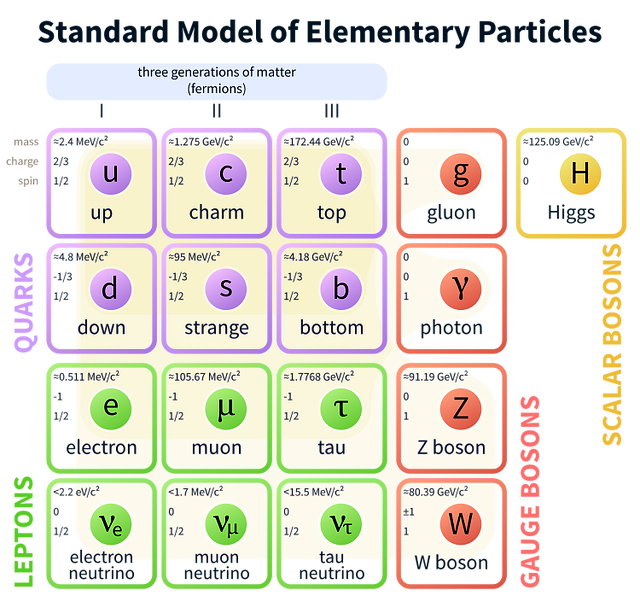
\includegraphics[scale=0.4]{sm}
  \caption[Standard Model of particle physics.]{Schematic representation of the Standard Model of particle physics. The SM is a theoretical model intended to describe three of the four fundamental forces of the universe in terms of a set of particles and their interactions. \cite{smpicture}.}
  \label{sm}
\end{figure}

The mathematical formulation of the SM is based on group theory and the use of Noether's theorem\cite{noether} which states that for a physical system modeled by a Lagrangian that is invariant under a group of transformations a conservation law is expected. For instance, a system described by a time-independent Lagrangian is invariant (symmetric) under time changes (transformations) with the total energy conservation law as the expected conservation law. In QED, the charge operator (Q) is the generator of the U(1) symmetry which according to the Noether's theorem means that there is a conserved quantity; this conserved quantity is the electric charge and thus the law conservation of electric charge is established.

In the SM, the symmetry group $SU(3)_C\otimes SU(2)_L\otimes U(1)_Y$ describes three of the four fundamental interactions in nature (see Section \ref{fund_inter}): strong interaction (SI), weak interaction (WI) and electromagnetic interactions (EI) in terms of symmetries associated to physical quantities:
\begin{itemize}
\item Strong: $SU(3)_C$ associated to color charge
\item Weak: $SU(2)_L$ associated to weak isospin and chirality
\item Electromagnetic: $U(1)_Y$ associated to weak hypercharge and electric charge
\end{itemize}

It will be shown that the electromagnetic and weak interactions are combined in the so-called electroweak interaction where chirality, hypercharge, weak isospin and electric charge are the central concepts.

\subsection{Fermions}\label{fermions}

The basic constituents of the ordinary matter at the lowest level, which form the set of elementary particles in the SM formulation, are quarks and leptons. All of them have spin 1/2, therefore they are classified as fermions since they obey Fermi-Dirac statistics. There are six ``flavors'' of quarks and three of leptons organized in three generations, or families, as shown in Table \ref{flav_gen}.\\
 
\begin{center}
\begin{table}[h!]
\centering
\footnotesize
\begin{tabular}{ccccc} \hline
                         &         & \multicolumn{3}{c}{Generation}                                                           \\ \hline
                         &Type     & 1st                          & 2nd                        & 3rd                          \\ \hline
\multirow{2}{*}{Leptons} &Charged  & Electron (e)                 & Moun($\mu$)                & Tau ($\tau$)                 \\%\hline
                         &Neutral  & Electron neutrino ($\nu_e$)  & Muon neutrino ($\nu_{\mu}$) & Tau neutrino ($\nu_{\tau}$) \\\hline
\multirow{2}{*}{Quarks}  &Up-type  & Up (u)                       & Charm (c)                & Top (t)                        \\%\hline
                         &Down-type& Down (d)                     & Strange (s)              & Bottom (b)                     \\\hline
\end{tabular}
\caption[Fermions of the SM.]{Fermions of the SM. There are six flavors of quarks and three of leptons, organized in three generations, or families, composed of two pairs of closely related particles. The close relationship is motivated by the fact that each pair of particles is a member of an $SU(2)_L$ doublet that has an associated invariance under isospin transformations. WI between leptons is limited to the members of the same generation; WI between quarks is not limited but greatly favored, to same generation members. }\label{flav_gen}
\end{table}
\end{center}

There is a mass hierarchy between generations (see Table \ref{f_masses}), where the higher generation particles decays to the lower one, which can explain why the ordinary matter is made of particles from the first generation. In the SM, neutrinos are modeled as massless particles so they are not subject to this mass hierarchy; however, today it is known that neutrinos are massive so the hierarchy could be restated. The reason behind this mass hierachy is one of the most important open questions in particle physics, and it becomes more puzzling when noticing that the mass difference between first and second generation fermions is small compared to the mass difference with respect to the third generation.
\begin{center}
\begin{table}[h]
\centering
\footnotesize
\begin{tabular}{lclc} \hline
Lepton    & Mass (MeV/c$^2$) & Quark  & Mass (MeV/c$^2$)       \\ \hline
e         & 0.51             & u      & $ 2.2$             \\ %\hline
$\mu$     & 105.65           & c      & $ 1.28\times 10^3$ \\ %\hline
$\tau$    & 1776.86          & t      & $ 173.1\times 10^3$\\ %\hline
$\nu_e$   & Unknown          & d      & $ 4.7$             \\ %\hline
$\nu_\mu$ & Unknown          & s      & $ 96$              \\ %\hline
$\tau_\mu$& Unknown          & b      & $ 4.18\times 10^3$ \\ \hline
\end{tabular}
\caption[Fermion masses.]{Fermion masses\cite{pdg}. Generations differ by mass in a way that has been interpreted as a masss hierarchy. Approximate values with no uncertainties are used, for comparison purpose.}\label{f_masses}
\end{table}
\end{center}

Usually, the second and third generation fermions are produced in high energy processes, like the ones recreated in particle accelerators.         

\subsubsection{Leptons}

A lepton is an elementary particle that is not subject to the SI. As seen in Table \ref{flav_gen}, there are two types of leptons, the charged ones (electron, muon and tau) and the neutral ones (the three neutrinos). The electric charge (Q) is the property that gives leptons the ability to participate in the EI. From the classical point of view, Q plays a central role determining, among others, the strength of the electric field through which the electromagnetic force is exerted. It is clear that neutrinos are not affected by EI because they don't carry electric charge.

Another feature of the leptons that is fundamental in the mathematical description of the SM is the chirality, which is closely related to spin and helicity. Helicity defines the handedness of a particle by relating its spin and momentum such that if they are parallel then the particle is right-handed; if spin and momentum are antiparallel the particle is said to be left-handed. The study of parity conservation (or violation) in $\beta$-decay has shown that only left-handed electrons/neutrinos or right-handed positrons/anti-neutrinos are created\cite{goldhaber}; the inclusion of that feature in the theory was achieved by using projection operators for helicity, however, helicity is frame dependent for massive particles which makes it not Lorentz invariant and then another related attribute has to be used: \textit{chirality}.

Chirality is a purely quantum attribute which makes it not so easy to describe in graphical terms but it defines how the wave function of a particle transforms under certain rotations. As with helicity, there are two chiral states, left-handed chiral (L) and right-handed chiral (R). In the highly relativistic limit where $E\approx p \gg m$ helicity and chirality converge, becoming exactly the same for massless particles.

In the following, when referring to left-handed (right-handed) it will mean left-handed chiral (right-handed chiral). The fundamental fact about chirality is that while EI and SI are not sensitive to chirality, in WI left-handed and right-handed fermions are treated asymmetrically, such that only left-handed fermions and right-handed anti-fermions are allowed to couple to WI mediators, which is a violation of parity. The way to translate this statement in a formal mathematical formulation is based on the isospin symmetry group $SU(2)_L$.

Each generation of leptons is seen as a weak isospin doublet.\footnote{The weak isospin is an analogy of the isospin symmetry in strong interaction where neutron and proton are affected equally by strong force but differ in their charge.} The left-handed charged lepton and its associated left-handed neutrino are arranged in doublets of weak isospin T=1/2 while their right-handed partners are singlets:

\begin{equation}
\binom{\nu_l}{l}_L , l_R := \binom{\nu_e}{e}_L , \binom{\nu_\mu}{\mu}_L, \binom{\nu_\tau}{\tau}_L, e_R, \mu_R, \tau_R, \nu_{eR}, \nu_{\mu R}, \nu_{\tau R}
\label{lepton_multiplets}
\end{equation}

The isospin third component refers to the eigenvalues of the weak isospin operator which for doublets is $T_3 = \pm 1/2$, while for singlets it is $T_3=0$. The physical meaning of this doublet-singlet arrangement falls in that the WI couples the two particles in the doublet by exchanging the interaction mediator while the singlet member is not involved in WI. The main properties of the leptons are summarized in Table \ref{leptons}.

%% When two leptons interact, the interaction involves only one kind of lepton \ie at the vertex both lepton lines refers to the same kind of lepton (see Figure. \ref{lepton_int}), therefore EI does not change flavor; the so-called ``Lepton number'' was assigned to each lepton flavor: 

%% \begin{itemize}    
%% \item Electron number: $N_e=N(e^-) - N(e^+)$
%% \item Muon number    : $N_\mu=N(\mu^-) - N(\mu^+)$
%% \item Tau number     : $N_\tau=N(\tau^-) - N(\tau^+)$
%% \end{itemize}

%% representing the number of leptons plus the number of anti-leptons of each flavor entering in a process. These lepton number are conserved in EI and SI since those interactions don't change flavor. 

%% \begin{figure}[h!]
%%   \centering
%%   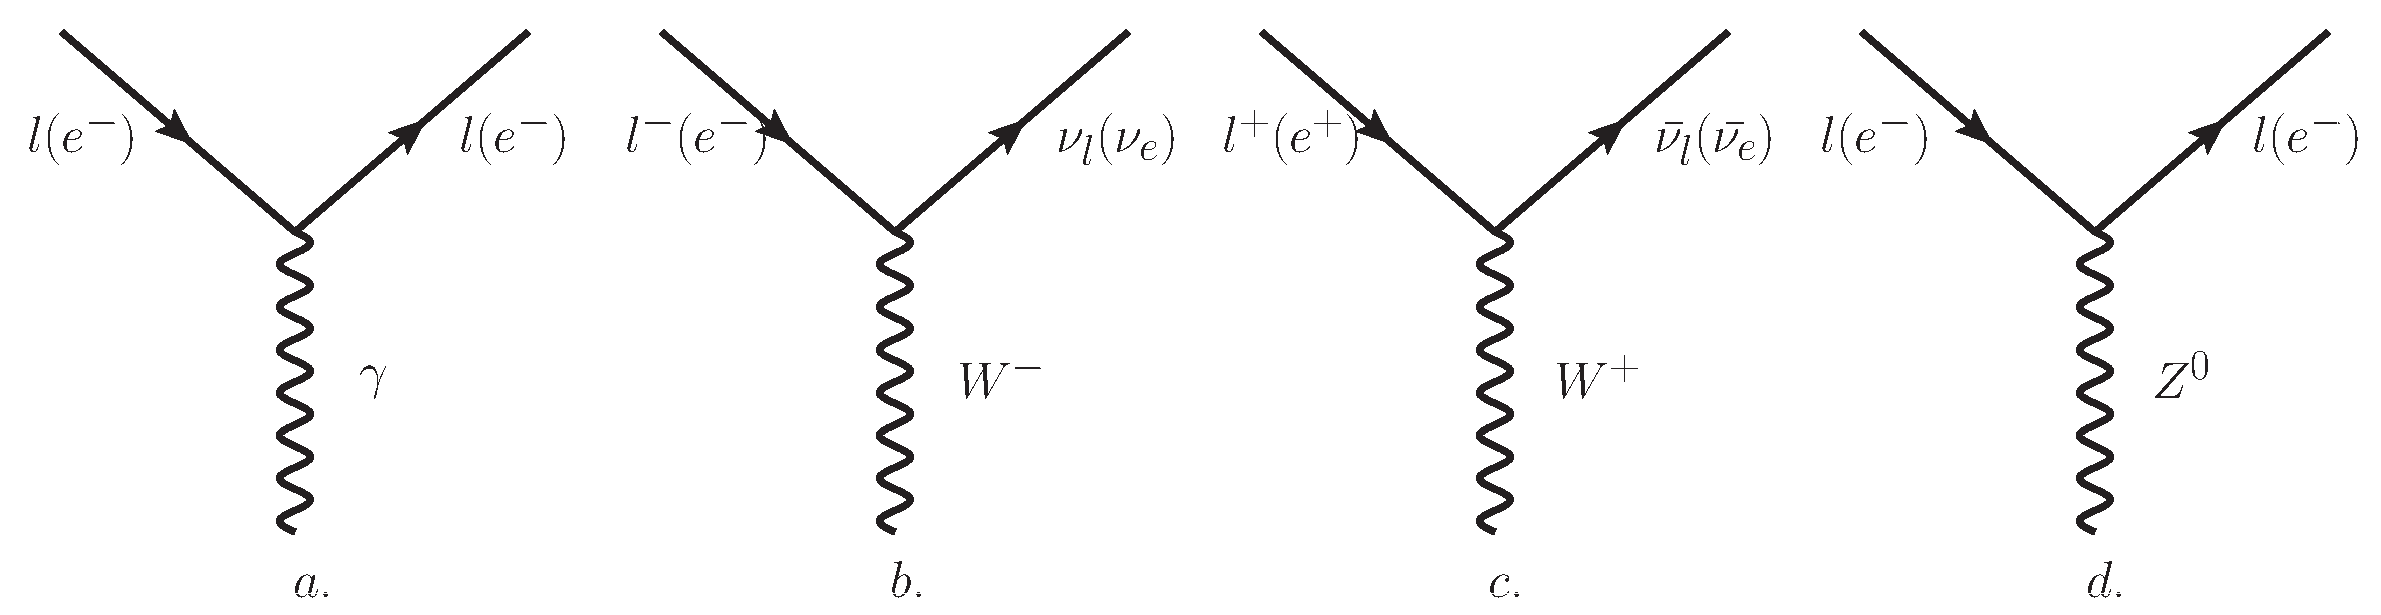
\includegraphics[scale=0.4]{lepton_int}
%%   \caption[Leptons interactions]{Diagrams representing the leptons interactions with the gauge fields; a: EI-electron and photon; b,c,d: WI - first generation leptons.}
%%   \label{lepton_int}
%% \end{figure}

%% The lepton number definition has to be extended when considering the WI. The new definition is given in terms of the generation's weak isospin doublets, thus, electron and electron neutrino have electron number $L_e=1$, muon and muon neutrino have muon number $L_\mu=1$, tau and tau neutrino have tau number $L_\tau=1$. Lepton number conservation, which now is SM wide, implies that leptons have to be created in pairs.

Altough all three flavor neutrinos have been observed, their masses remain unknown and only some estimations have been made\cite{nu_mass}. The main reason is that the flavor eigenstates are not the same as the mass eigenstates which implies that when a neutrino is created its mass state is a linear combination of the three mass eigenstates and experiments can only probe the squared difference of the masses. The Pontecorvo-Maki-Nakagawa-Sakata (PMNS) mixing matrix encodes the relationship between flavor and mass eigenstates.
\begin{center}
\begin{table}[h]
\centering
\footnotesize
\begin{tabular}{lcccccc} \hline
Lepton                      & Q(e) & $T_3$&$L_e$ & $L_\mu$ & $L_\tau$ & Lifetime (s)                \\ \hline
Electron (e)                & -1   & -1/2 & 1    & 0       & 0        & Stable                      \\ %\hline
Electron neutrino($\nu_e$)  & 0    &  1/2 & 1    & 0       & 0        & Unknown                     \\ %\hline
Muon ($\mu$)                & -1   & -1/2 & 0    & 1       & 0        & $2.19\times10^{-6}$\\ %\hline
Muon neutrino ($\nu_\mu$)   & 0    &  1/2 & 0    & 1       & 0        & Unknown                     \\ %\hline
Tau ($\tau$)                & -1   & -1/2 & 0    & 0       & 1        & $290.3\times10^{-15}$    \\ %\hline
Tau neutrino ($\tau_\mu$)   & 0    &  1/2 & 0    & 0       & 1        & Unknown                     \\ \hline
\end{tabular}
\caption[Lepton properties.]{Lepton properties\cite{pdg}. Q: electric charge, $T_3$: weak isospin. Only left-handed leptons and right-handed anti-leptons participate in the WI. Anti-particles with inverted $T_3$, Q and lepton number complete the leptons set but are not listed. Right-handed leptons and left-handed anti-leptons, neither listed, form weak isospin singlets with $T_3=0$ and do not take part in the weak interaction.}\label{leptons}
\end{table}
\end{center}

\subsubsection{Quarks}

Quarks are the basic constituents of protons and neutrons. The way quarks join to form bound states, called ``hadrons'', is through the SI. Quarks are affected by all the fundamental interactions which means that they carry all the four types of charges: color, electric charge, weak isospin and mass.

\begin{center}
\begin{table}[h!]
\centering
\footnotesize
\begin{tabular}{lcccccccccc} \hline
Flavor     & Q(e) & $I_3$ & $T_3$  & B   & C & S  & T & B'  & Y    & Color \\ \hline
Up (u)     & 2/3  & 1/2   &  1/2   & 1/3 & 0 & 0  & 0 & 0   & 1/3  & r,b,g \\ %\hline
Charm (c)  & 2/3  & 0     &  1/2   & 1/3 & 1 & 0  & 0 & 0   & 4/3  & r,b,g \\ %\hline
Top(t)     & 2/3  & 0     &  1/2   & 1/3 & 0 & 0  & 1 & 0   & 4/3  & r,b,g \\ \hline
Down(d)    & -1/3 & -1/2  & -1/2   & 1/3 & 0 & 0  & 0 & 0   & 1/3  & r,b,g \\ %\hline
Strange(s) & -1/3 & 0     & -1/2   & 1/3 & 0 & -1 & 0 & 0   & -2/3 & r,b,g \\ %\hline
Bottom(b)  & -1/3 & 0     & -1/2   & 1/3 & 0 & 0  & 0 & -1  & -2/3 & r,b,g \\ \hline
\end{tabular}
\caption[Quark properties.]{Quark properties \cite{pdg}. Q: electric charge, $I_3$: isospin, $T_3$: weak isospin, B: baryon number, C: charmness, S: strangeness, T: topness, B': bottomness, Y: hypercharge. Anti-quarks posses the same mass and spin as quarks but all charges (color, flavor numbers) have opposite sign.}\label{quarks}
\end{table}
\end{center}

Table \ref{quarks} summarizes the features of quarks, among which the most remarkable is their fractional electric charge. Note that fractional charge is not a problem, given that quarks are not found isolated, but serves to explain how composed particles are formed out of two or more valence quarks\footnote{Hadrons can contain an indefinite number of virtual quarks and gluons, known as the quark and gluon sea, but only the valence quarks determine hadrons' quantum numbers.}.

Color charge is responsible for the SI between quarks and is the symmetry ($SU(3)_C$) that defines the formalism to describe SI. There are three colors: red (r), blue (b) and green (g) and their corresponding three anti-colors; thus each quark carries one color unit while anti-quarks carries one anti-color unit. As explained in Section \ref{fund_inter}, quarks are not allowed to be isolated due to the color confinement effect, hence, their features have been studied indirectly by observing their bound states created when

\begin{itemize}
\item one quark with a color charge is attracted by an anti-quark with the corresponding anti-color charge forming a colorless particle called a ``meson.''
\item three quarks (anti-quarks) with different color (anti-color) charges are attracted among them forming a colorless particle called a ``baryon (anti-baryon).''          
\end{itemize}

In practice, when a quark is left alone isolated a process called ``hadronization'' occurs where the quark emits gluons (see Section \ref{sec:gb}) which eventually will generate new quark-antiquark pairs and so on; those quarks will recombine to form hadrons that will decay into leptons. This proliferation of particles looks like a ``jet'' coming from the isolated quark. More details about the hadronization process and jet structure will be given in chapter\ref{ch:gensimreco}.         

In the first version of the quark model (1964), M. Gell-Mann\cite{gellman} and G. Zweig\cite{zweig,zweig2} developed a consistent way to classify hadrons according to their properties. Only three quarks (u, d, s) were involved in a scheme in which all baryons have baryon number B=1 and therefore quarks have B=1/3; non-baryons have B=0. Baryon number is conserved in SI and EI which means that single quarks cannot be created but in pairs $q-\bar{q}$.

The scheme organizes baryons in a two-dimensional space ($I_3$ - Y); Y (hypercharge) and $I_3$ (isospin) are quantum numbers related by the Gell-Mann-Nishijima formula\cite{gell_ni,gell_ni2}:
\begin{equation}
Q=I_3 + \frac{Y}{2}
\label{gmn}
\end{equation}

\noindent where $Y=B+S+C+T+B'$ are the quantum numbers listed in Table \ref{quarks}. 

There are six quark flavors organized in three generations (see Table \ref{flav_gen}) following a mass hierarchy which, again, implies that higher generations decay to first generation quarks.

\begin{center}
\begin{table}[h!]
\centering
\footnotesize
\begin{tabular}{ccccccccccc} \hline
                          &     \multicolumn{3}{c}{Quarks}                       & $T_3$              & $Y_W$&  \multicolumn{3}{c}{Leptons}                                              & $T_3$                    & $Y_W$\\\hline
Doublets                  & $\binom{u}{d'}_L$& $\binom{c}{s'}_L$& $\binom{t}{b'}_L$& $\binom{1/2}{-1/2}$& 1/3  & $\binom{\nu_e}{e}_L$ & $\binom{\nu_\mu}{\mu}_L$& $\binom{\nu_\tau}{\tau}_L$& $\binom{1/2}{-1/2}$ & -1    \\ %\hline \\%\hline 
\multirow{2}{*}{Singlets} & $u_R$            & $c_R$            & $t_R$            & 0                  & 4/3 & $\nu_{eR}$           & $\nu_{\mu R}$           & $\nu_{\tau R}$            &                     &       \\ % \\
                          & $d'_R$           & $s'_R$           & $b'_R$           & 0                  & -2/3 & $e_R$                & $\mu_R$                 & $\tau_R$                  & 0                   & -2   \\ \hline % \\ \hline
%% Leptons                   &                      &                         &                           &                     &       \\ \hline
%% Doublets                  & $\binom{\nu_e}{e}_L$ & $\binom{\nu_\mu}{\mu}_L$& $\binom{\nu_\tau}{\tau}_L$& $\binom{1/2}{-1/2}$ & -1    \\%\hline 
%% \multirow{2}{*}{Singlets} & $\nu_{eR}$           & $\nu_{\mu R}$           & $\nu_{\tau R}$            &                     &       \\
%%                           & $e_R$                & $\mu_R$                 & $\tau_R$                  & 0                   & -2   \\ \hline
\end{tabular}
\caption[Fermion weak isospin and weak hypercharge multiplets.]{Fermion weak isospin and weak hypercharge multiplets. Weak hypercharge is calculated through the Gell-Mann-Nishijima formula \ref{gmn} but using the weak isospin and charge for quarks.}\label{T3Y}
\end{table}
\end{center}

Isospin doublets of quarks are also defined (see Table \ref{T3Y}), and same as for neutrinos, the WI eigenstates are not the same as the mass eigenstates which means that members of different quark generations are connected by the WI mediator; thus, up-type quarks are coupled not to down-type quarks (the mass eigenstates) directly but to a superposition of down-type quarks $(q'_d; the weak eigenstates)$ via WI according to: 

$$q'_d = V_{CKM}\hspace{0.1cm}q_d$$
\begin{equation}
\begin{pmatrix}d'\\ s'\\ b'\end{pmatrix}=\begin{pmatrix} V_{ud} & V_{us} & V_{ub}\\ V_{cd} & V_{cs} & V_{cb}\\ V_{td} & V_{ts} & V_{tb}\end{pmatrix}\begin{pmatrix}d\\s\\b\end{pmatrix}
\label{eq:qmixing}
\end{equation}

\noindent where $V_{CKM}$ is known as Cabibbo-Kobayashi-Maskawa (CKM) mixing matrix\cite{C,KM} given by  

\begin{equation}
\begin{pmatrix}
|V_{ud}| & |V_{us}| & |V_{ub}| \\
|V_{cd}| & |V_{cs}| & |V_{cb}| \\
|V_{td}| & |V_{ts}| & |V_{tb}|
\end{pmatrix} = \begin{pmatrix}
0.97427 \pm 0.00015 & 0.22534 \pm 0.00065 & 0.00351^{+0.00015}_{-0.00014} \\
0.22520 \pm 0.00065 & 0.97344 \pm 0.00016 & 0.0412^{+0.0011}_{-0.0005} \\
0.00867^{+0.00029}_{-0.00031} & 0.0404^{+0.0011}_{-0.0005} & 0.999146^{+0.000021}_{-0.000046}
\end{pmatrix}.
\label{eq:ckm}
\end{equation}

\begin{figure}[!h]
  \centering
  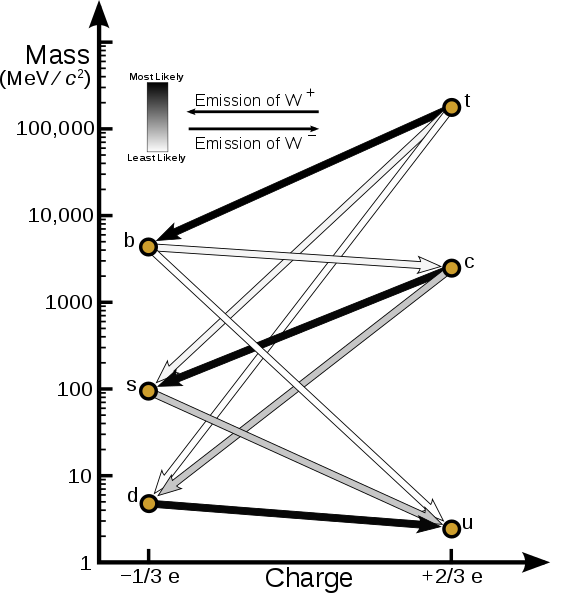
\includegraphics[scale=0.3]{quarks_decay}
  %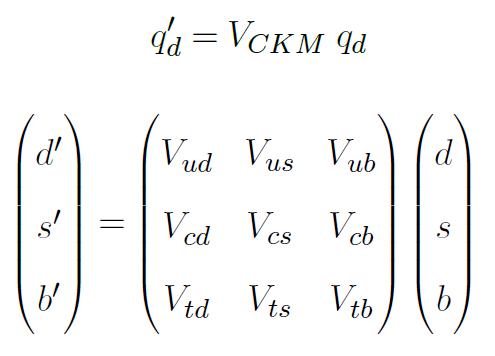
\includegraphics[width=0.45\textwidth]{ckm}
  \caption[Transformations between quarks]{Transformations between quarks through the exchange of a WI. Higher generations quarks decay to first generation quarks by emitting a W boson. The arrow color indicates the likelihood of the transition according to the grey scale in the top left side which represent the CKM matrix parameters\cite{ckm}.}
  \label{quarks_decay}
\end{figure}

The weak decays of quarks are represented in the diagram of Figure \ref{quarks_decay}; again the CKM matrix plays a central role since it contains the probabilities for the different quark decay channels, in particular, note that quark decays are greatly favored between generation members.\\

CKM matrix is a $3\times3$ unitary matrix parametrized by three mixing angles and the \textit{CP-mixing phase}; the latter is the parameter responsible for the Charge-Parity symmetry violation (CP-violation) in the SM. The fact that the top quark decays almost all the time to a bottom quark is exploited in this thesis when making the selection of the signal events by requiring the presence of a jet tagged as a jet coming from a $b$ quark in the final state.% The effect of the \textit{CP-mixing phase} on the cross section of associated production of Higss boson and a single top process is also explored in this thesis.    

\subsection{Fundamental interactions}\label{fund_inter}

\begin{figure}[h!]
  \centering
  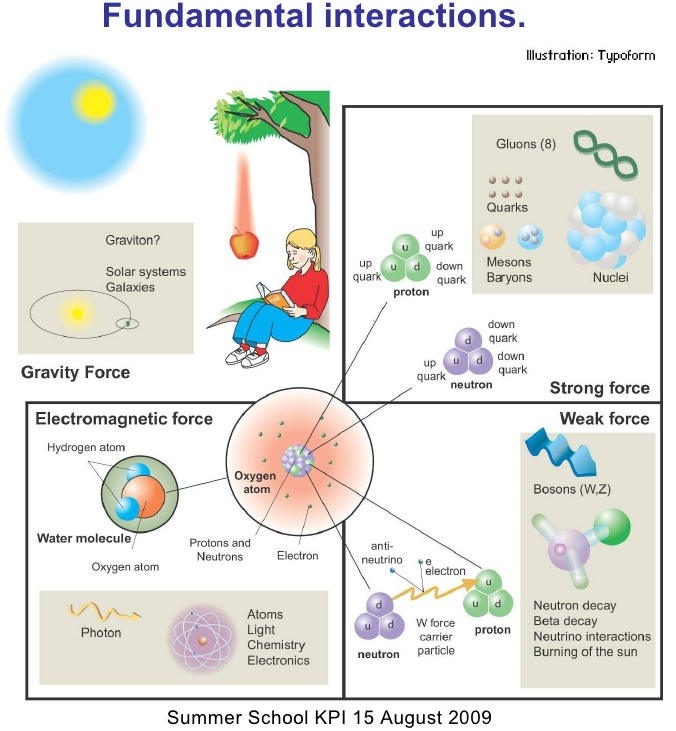
\includegraphics[scale=0.5]{fund_interac}
  \caption[Fundamental interactions in nature.]{Fundamental interactions in nature. Despite the many manifestations of forces in nature, we can track all of them back to one of the fundamental interactions. The most common forces are gravity and electromagnetic given that all of us are subject and experience them in everyday life.}
  \label{fund_interac}
\end{figure}

Even though there are many manifestations of force in nature, like the ones represented in Figure \ref{fund_interac}, we can classify all of them in four fundamental interactions:
\begin{itemize}

\item \textit{Electromagnetic interaction (EI)} affects particles that are ``electrically charged,'' like electrons and protons. It is described by QED, combining quantum mechanics, special relativity and electromagnetism in order to explain how particles with electric charge interact through the exchange of photons, therefore, one says that ``Electomagnetic Force'' is mediated by ``photons''. Figure \ref{fi_scatt}a. shows a graphical representation, known as ``Feynman diagram'', of electron-electron scattering.    

\item \textit{Strong interaction (SI)} described by Quantum Chromodynamics (QCD). Hadrons like proton and neutron have internal structure given that they are composed of two or more valence quarks\footnote{particles made of four and five quarks are exotic states not so common.}. Quarks have fractional electric charge which means that they are subject to electromagnetic interaction and in the case of the proton they should break appart due to electrostatic repulsion; however, quarks are held together inside the hadrons against their electrostatic repulsion by the ``Strong Force'' through the exchange of ``gluons.'' The analog to the electric charge is the ``color charge''. Electrons and photons are elementary particles as quarks but they don't carry color charge, therefore they are not subject to SI. The Feynman diagram for gluon exchange between quarks is shown in Figure \ref{fi_scatt}b.  

\begin{figure}[h!]
\centering
    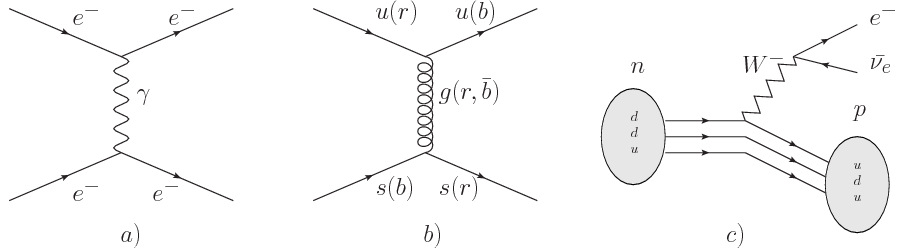
\includegraphics[scale=0.4]{fi_scatt}
\caption[SM interactions diagrams]{Feynman diagrams representing the interactions in SM; a) EI: e-e scattering; b) SI: gluon exchange between quarks ; c) WI: $\beta$-decay }
\label{fi_scatt}
\end{figure}

\item \textit{Weak interaction (WI)} described by the weak theory (WT), is responsible, for instance, for the radioactive decay in atoms and proton-proton (pp) fusion within the sun. Quarks and leptons are the particles affected by the weak interaction; they possess a property called ``flavor charge'' (see \ref{fermions}) which can be changed by emitting or absorbing one weak force mediator. There are three mediators of the ``weak force'' known as ``Z'' boson in the case of electrically neutral changes and ``$W^\pm$'' bosons in the case of electrically charged changes. The ``weak isospin'' is the WI analog to electric charge in EI, and color charge in SI, and defines how quarks and leptons are affected by the weak force. Figure \ref{fi_scatt}c. shows the Feynman diagram of $\beta$-decay where a newtron (n) is transformed in a proton (p) by emmiting a $W^-$ particle. Since this thesis is in the frame of the electroweak interaction, a more detailed description of it will be given in Section \ref{sec:EWI}

\item \textit{Gravitational interaction (GI)} described by General Theory of Relativity (GR). It is responsible for the structure of galaxies and black holes as well as the expansion of the universe. As a classical theory, in the sense that it can be formulated without even appeal to the concept of quantization, it implies that the spacetime is a continuum and predictions can be made without limitation to the precision of the measurement tools. The latter represent a direct contradiction of the quantum mechanics principles. Gravity is deterministic while quantum mechanics is probabilistic; despite that, efforts to develop a quantum theory of gravity have predicted the ``graviton'' as mediator of the Gravitational force\footnote{Actually a wide variety of theories have been developed in an attempt to describe gravity; some famous examples are string theory and supergravity.}.     
\end{itemize}

\begin{center}
\begin{table}[h!]
\centering
\scriptsize
\begin{tabular}{llm{1.2cm}ll}\hline%\hline
Interaction            & Acts on                         & Relative strength & Range (m)  & Mediators \\ \hline
Electromagnetic (QED)  & Electrically charged particles  & $10^{-2}$         & Infinite   & Photon    \\%\hline
Strong          (QCD)  & Quarks and gluons               & 1                 & $10^{-15}$ & Gluon     \\%\hline
Weak            (WI)   & Leptons and quarks              & $10^{-6}$         & $10^{-18}$ & \wpm, Z   \\%\hline
Gravitational   (GI)   & Massive particles               & $10^{-39}$        & Infinite   & Graviton  \\\hline
\end{tabular}
\caption[Fundamental interactions features.]{Fundamental interactions features\cite{hyperphys}. }\label{fund_inter_feat}
\end{table}
\end{center}

Table \ref{fund_inter_feat} sumarizes the main features of the fundamental interactions. The relative strength of the fundamental forces reveals the meaning of strong and weak; in a context where the relative strength of the SI is 1, the EI is about hundred times weaker and WI is about million times weaker thant the SI. A good description on how the relative strenght and range of the fundamental intreractions are calculated can be found in References \cite{hyperphys,matt}. In the everyday life, only EI and GI are explicitly experienced due to the range of these interactions; \ie, at the human scale distances only EI and GI have appreciable effects, in contrast to SI which at distances greater than $10^{-15}$m become negligible.\\                     

QED was built successfully on the basis of the classical electrodynamics theory (CED) of Maxwell and Lorentz, following theoretical and experimental requirements imposed by

\begin{itemize}
\item lorentz invariance: independence on the reference frame.  
\item locallity: interacting fields are evaluated at the same space-time point to avoid action at a distance. 
\item renormalizability: physical predictions are finite and well defined 
\item particle spectrum, symmetries and conservation laws already known must emerge from the theory.
\item gauge invariance.
\end{itemize}

The gauge invariance requirement reflects the fact that the fundamental fields cannot be directly measured but associated fields which are the observables. Electric (\textbf{``E''}) and magnetic (\textbf{``B''}) fields in CED are associated with the electric scalar potential ``V'' and the vector potential \textbf{``A''}. In particular, \textbf{E} can be obtained by measuring the change in the space of the scalar potential (\textbf{$\Delta$}V); however, two scalar potentials differing by a constant ``f'' correspond to the same electric field. The same happens in the case of the vector potential \textbf{``A''}; thus, different configurations of the associated fields result in the same set of values of the observables. The freedom in choosing one particular configuration is known as ``gauge freedom''; the tranformation law connecting two configurations is known as ``gauge transformation'' and the fact that the observables are not affected by a gauge transformation is called ``gauge invariance''.\\

When the gauge tranformation:  

\begin{align}\label{cov_der}
\textbf{A} \to &\textbf{A} -\Delta f\nonumber\\
V \to & V - \frac{\partial f}{\partial t}
\end{align}

\noindent is applied to Maxwell equations, they are still satisfied and the fields remain invariant. Thus, CED is invariant under gauge transformations and is called a ``gauge theory''. The set of all gauge transformations form the ``symmetry group'' of the theory, which according to the group theory, has a set of ``group generators''. The number of group generators determine the number of ``gauge fields'' of the theory.\\

As mentioned in the first lines of Section \ref{secc:SM}, QED has one symmetry group (U(1)) with one group generator (the Q operator) and one gauge field (the electromagnetic field $A^\mu$). In CED there is not a clear definition, beyond the historical convention, of which fields are the fundamental and which are the associated, but in QED it is clear that the fundamental field is $A^\mu$. When a gauge theory is quantized, the gauge field is quantized and its quanta is called ``gauge boson''. The word boson characterizes particles with integer spin which obvey Bose-einstein statistics.\\      

As will be detailed in Section \ref{sec:EWI}, interactions between partcles in a system can be obtained by considering first the Lagrangian density of free particles in the system, which of course is incomplete because the interaction terms have been left out, and demanding global phase transformation invariance. Global phase transformation invariance means that a gauge transformation is performed identically to every point in the space\footnote{Here space corresponds to the 4-dimensional space \ie space-time.} and the Lagrangian remains invariant. Then, the global transformation is promoted to a local phase transformation (this time the gauge transformation depends on the position in space) and again invariance is required.\\

Due to the space dependence of the local tranformation, the Lagrangian density is not invariant anymore. In order to restate the gauge invariance, the gauge covariant derivative is introduced in the Lagrangian and with it the gauge field responsible for the interaction between particles in the system. The new Lagrangian density is gauge invariant, includes the interaction terms needed to account for the interactions and provides a way to explain the interaction between particles through the exchange of the gauge boson.

This recipe was used to build QED and the theories that aim to explain the fundamental interactions.   

\subsection{Gauge bosons}\label{sec:gb}

The importance of the gauge bosons comes from the fact that they are the force mediators or force carriers. The features of the gauge bosons reflect those of the fields they represent and they are extracted from the Lagrangian density used to describe the interactions. In Section \ref{sec:EWI}, it will be shown how the gauge bosons of the EI and WI emerge from the electroweak Lagrangian. The SI gauge bosons features are also extracted from the SI Lagrangian but it is not detailed in this document. The main features of the SM gauge bosons will be briefly presented below and summarized in Table \ref{gauge_boson}.

\begin{itemize} 
\item \textbf{Photon}. EI occurs when the photon couples to (is exchanged between) particles carrying electric charge; however, the photon itself does not carry electric charge, therefore, there is no coupling between photons. Given that the photon is massless the EI is of infinite range, \ie, electrically charged particles interact even if they are located far away one from each other; this also implies that photons always move with the speed of light. 

\item \textbf{Gluon}. SI is mediated by gluons which, same as photons, are massless. They carry one unit of color charge and one unit of anticolor charge which means that gluons couple to other gluons. As a result, the range of the SI is not infinite but very short due to the attraction between gluons, giving rise to the ``color confinement'' which explains why color charged particles cannot be isolated but live within composited particles, like quarks inside protons. 

\item  \textbf{W, Z}. The WI mediators, $\wpm$ and Z, are massive which explains their short-range. Given that the WI is the only interaction that can change the flavor of the interacting particles, the W boson is the responsible for the nuclear transmutation where a neutron is converted in a proton or vice versa with the involvement of an electron and a neutrino (see Figure \ref{fi_scatt}c). The Z boson is the responsible of the neutral weak processes like neutrino elastic scattering where no electric charge but momentum transference is involved. WI gauge bosons carry isospin charge which makes posible the interaction between them.  
\end{itemize}

\begin{center}
\begin{table}[h!]
\centering
\scriptsize
\begin{tabular}{llllll}\hline%\hline
Interaction            & Mediator          & Electric charge (e) & Color charge & Weak Isospin & mass (GeV/c$^2$)   \\ \hline
Electromagnetic        & Photon ($\gamma$) & 0                   & No           & 0            & 0                  \\%\hline
Strong                 & Gluon (g)         & 0                   & Yes -octet   & No           & 0                  \\%\hline
\multirow{2}{*}{Weak}  & \wpm              & $\pm 1$             & No           & $\pm 1$      & 80.385 $\pm$ 0.015 \\%\hline
                       & Z                 & 0                   & No           & 0            & 91.188 $\pm$ 0.002 \\\hline
\end{tabular}
\caption[SM gauge bosons.]{SM gauge bosons main features\cite{pdg}.}\label{gauge_boson}
\end{table}
\end{center}

\section{Electroweak unification and the Higgs mechanism}\label{sec:EWI}

Physicists dream of building a theory that contains all the interactions in one single interaction, \ie, showing that at some scale in energy all the four fundamental interactions are unified and only one interaction emerges in a ``Theory of everything''. The first sign of the feasibility of such unification comes from success in the construction of the CED. Einstein spent years trying to reach that dream, which by 1920 only involved electromagnetism and gravity, with no success; however, a new partial unification was achieved in the 1960's, when S.Glashow\cite{glashow}, A.Salam\cite{salam} and S.Weinberg \cite{weinberg} independently proposed that electromagnetic and weak interactions are two manifestations of a more general interaction called ``electroweak interaction (EWT)''. Both, QCD and EWT, were developed in parallel and following the useful prescription provided by QED and the gauge invariance principles.\\

\begin{figure}[h!]
  \centering
  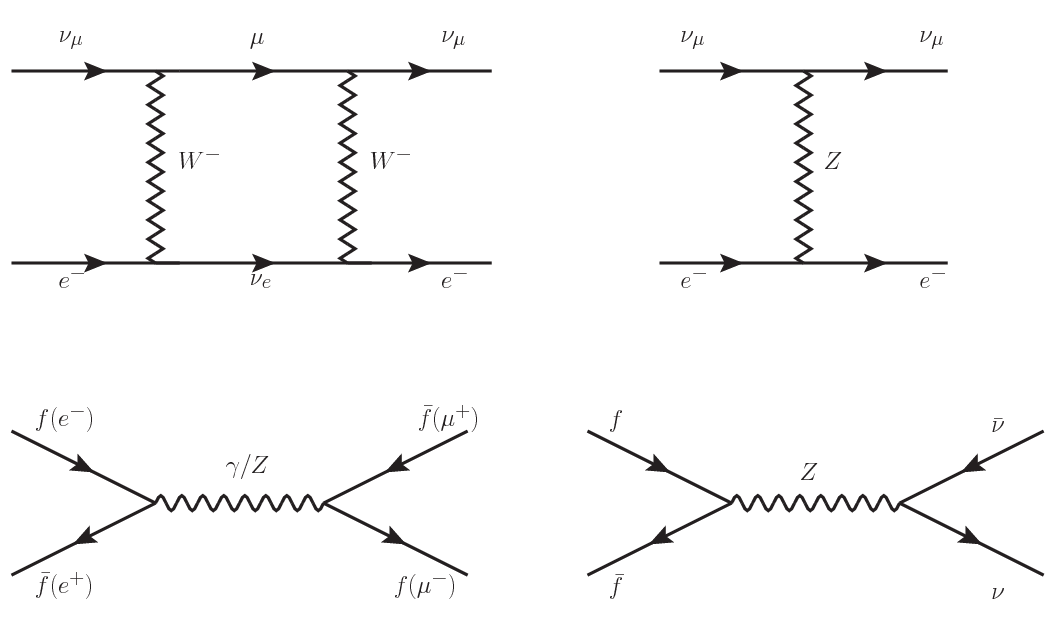
\includegraphics[scale=0.4]{nc}
  \caption[Neutral current processes]{Top: $\nu_{\mu}-e^-$ scattering going through charged currents (left) and neutral currents (right). Bottom: neutral current processes for charged fermions (left) and involving neutrinos (right). While neutral current processes involving only charged fermions can proceed through EI or WI, those involving neutrinos can only proceed via WI.}% The former can be seen as an indication that at some level WI and EI are closely connected.}
         \label{nc}
\end{figure}
         
The theory of weak interactions was capable of explaining the $\beta$-decay and in general the processes mediated by \wpm bosons. However, there were some processes like the ``$\nu_\mu - e$ scattering'' which would require the exchange of two W bosons (see Figure \ref{nc} top diagrams) giving rise to divergent loop integrals and then non finite predictions. By including neutral currents involving fermions via the exchange of neutral bosons Z, those divergences are compensated and the predictions become realistic.\\

Neutral weak interaction vertices conserve flavor in the same way as the electromagnetic vertices do, but additionally, the Z boson can couple to neutrinos which implies that processes involving charged fermions can proceed through EI or WI but processes involving neutrinos can proceed only through WI.\\   

The prescription to build a gauge theory of the WI consists of proposing a free field Lagrangian density that includes the particles involved; next, by requesting invariance under global phase transformations first and generalizing to local phase transformations invariance later, the conserved currents are identified and interactions are generated by introducing gauge fields. Given that the goal is to include the EI and WI in a single theory, the group symmetry considered should be a combination of $SU(2)_L$ and $U(1)_{em}$ , however the latter cannot be used directly because the EI treats left and right-handed particles indistinctly in contrast to the former. Fortunately, the weak hypercharge, which is a combination of the weak isospin and the electric charge (eqn \ref{gmn}) is suitable to be used since it is conserved by the  EI and WI. Thus, the symmetry group to be considered is

\begin{equation}
G\equiv SU(2)_L\otimes U(1)_Y
\end{equation}

 The following treatment applies to any of the fermion generations, but for simplicity the first generation of leptons will be considered\cite{peskin,mandl,halzen,pich}.\\

Given the first generation of leptons 

\begin{equation}\label{first_gen}
\psi_1 = \binom{\nu_e}{e^-}_L , \qquad \psi_2= \nu_{eR}, \qquad \psi_3= e^-_R
\end{equation}

\noindent the charged fermionic currents are given by

\beqn\label{fermion_currents}
J_\mu \equiv  J_\mu^+ = \bar{\nu}_{eL} \gamma_\mu e_L, \qquad J_\mu^\dagger \equiv J_\mu^- = \bar{e}_L \gamma_\mu \nu_{eL} 
\eeqn

\noindent and the free Lagrangian is given by

\begin{equation}\label{lo}
\Lagr_0 = \sum_{j=1}^3 i\overline{\psi}_j(x)\gamma^\mu \partial_\mu \psi_j(x).
\end{equation}

Mass terms are included directly in the QED and QCD free Lagrangians since they preserve the invariance under the symmetry transformations involved which treat left-handed and right-handed similarly, however mass terms of the form

\beqn 
m_W^2W_\mu^\dagger(x)W^\mu(x) + \frac{1}{2}m_Z^2Z_\mu(x)Z^\mu(x) -m_e\bar{\psi_e}(x)\psi_e(x)
\eeqn
\noindent which represent the mass of \wpm, Z and electrons, are not invariant under G transformations, therefore the gauge fields described by the EWI are in principle massless.\\

Experiments have shown that the gauge fields are not massless; however, they have to acquire mass through a mechanism compatible with the gauge invariance; that mechanism is known as the ``Higgs mechanism'' and will be considered later in this Section. The global transformations in the combined symmetry group G can be written as

\begin{align}\label{G_transf}
\psi_1(x) \xrightarrow[]{G}\psi'_1(x)\equiv &U_YU_L\psi_1(x),\nonumber\\ 
\psi_2(x) \xrightarrow[]{G}\psi'_2(x)\equiv &U_Y\psi_2(x),\\
\psi_3(x) \xrightarrow[]{G}\psi'_3(x)\equiv &U_Y\psi_3(x)\nonumber
\end{align}
\noindent where $U_L$ represent the $SU(2)_L$ transformation acting only on the weak isospin doublet and $U_Y$ represent the $U(1)_Y$ transformation acting on all the weak isospin multiplets. Explicitly
\beqn
U_L\equiv \exp \left(i\frac{\sigma_i}{2}\alpha^i\right), \qquad U_Y\equiv \exp(iy_i\beta) \qquad (i=1,2,3)
\eeqn
\noindent with $\sigma_i$ the Pauli matrices and $y_i$ the weak hypercharges. In order to promote the transformations from global to local while keeping the invariance, it is required that $\alpha^i=\alpha^i(x)$, $\beta=\beta(x)$ and the replacement of the ordinary derivatives by the covariant derivatives

\begin{align}\label{cov_der2}
D_\mu \psi_1(x) \equiv &\left[\partial_\mu + ig\sigma_i W_\mu^i(x)/2+ ig'y_1B_\mu(x)\right]\psi_1(x)\nonumber\\ 
D_\mu \psi_2(x) \equiv &\left[\partial_\mu + ig'y_2B_\mu(x)\right]\psi_2(x)\\
D_\mu \psi_3(x) \equiv &\left[\partial_\mu + ig'y_3B_\mu(x)\right]\psi_3(x)\nonumber 
\end{align}

\noindent introducing in this way four gauge fields, $W_\mu^i(x)$ and $B_\mu(x)$, in the process. The covariant derivatives (eqn \ref{cov_der2}) are required to transform in the same way as fermion fields $\psi_i(x)$ themselves, therefore, the gauge fields transform as:

\begin{align}\label{f_transf}
B_\mu(x) \xrightarrow[]{G} B_\mu'(x)\equiv & B_\mu(x)
- \frac{1}{g'}\partial_\mu\beta(x) \nonumber\\
W^i_\mu(x) \xrightarrow[]{G} W_\mu^{i\prime}(x)\equiv & W^i_\mu(x) - \frac{i}{g}\partial_\mu \alpha_i(x) - \varepsilon_{ijk}\alpha_i(x)W^i_\mu(x).
\end{align}

The G invariant version of the Lagrangian density \ref{lo} can be written as

\begin{equation}\label{linv}
\Lagr_0 = \sum_{j=1}^3 i\overline{\psi}_j(x)\gamma^\mu D_\mu \psi_j(x)
\end{equation}

\noindent where free massless fermion and gauge fields and fermion-gauge boson interactions are included. The EWI Lagrangian density must additionally include kinetic terms for the gauge fields ($\Lagr_G$) which are built from the field strengths, according to

\begin{align}
B_{\mu\nu}(x)   \equiv & \partial_\mu B_\nu -  \partial_\nu B_\mu \label{B_tensor} \\ 
W^i_{\mu\nu}(x) \equiv & \partial_\mu W^i_\nu(x) - \partial_\nu W^i_\mu(x) - g\varepsilon^{ijk}W^j_\mu W^k_\nu \label{W_tensor}
\end{align}

\noindent the last term in eqn. \ref{W_tensor} is added in order to hold the gauge invariance; therefore,

\beqn\label{lg}
\Lagr_G = -\frac{1}{4}B_{\mu\nu}(x)B^{\mu\nu}(x)-\frac{1}{4}W^i_{\mu\nu}(x)W_i^{\mu\nu}(x)
\eeqn

\noindent which contains not only the free gauge fields contributions, but also the gauge fields self-interactions and interactions among them.\\  

The three weak isospin conserved currents resulting from the $SU(2)_L$ symmetry are given by

\beqn
J_\mu^i(x)=\frac{1}{2}\bar{\psi_1}(x)\gamma_\mu \sigma^i \psi_1(x) 
\eeqn

\noindent while the weak hypercharge conserved current resulting from the $U(1)_Y$ symmetry is given by 

\beqn
J_\mu^Y = \sum_{j=1}^3 \overline{\psi}_j(x)\gamma_\mu y_j\psi_j(x)
\eeqn

In order to evaluate the electroweak interactions modeled by an isotriplet field $W^i_\mu$ which couples to isospin currents $J^i_\mu$ with strength $g$ and additionally the singlet field $B_\mu$ which couples to the weak hypercharge current $J_\mu^Y$ with strength $g'/2$. The interaction Lagrangian density to be considered is

\beqn
\Lagr_I = -gJ^{i\mu}(x)W_\mu^i(x)- \frac{g'}{2}J^{Y\mu}(x)B_\mu(x)
\eeqn

%\noindent written in terms of the physical fields $\wpm_\mu$, $Z_\mu$ and $A_\mu$.

Note that the weak isospin currents are not the same as the charged fermionic currents that were used to describe the WI (eqn \ref{fermion_currents}), since the weak isospin eigenstates are not the same as the mass eigenstates, but they are closely related

\beqn\label{fermion_currents2}
J_\mu = \frac{1}{2}(J_\mu^1 + iJ_\mu^2) ,  \qquad  J_\mu^\dagger = \frac{1}{2}(J_\mu^1 - iJ_\mu^2).
\eeqn

The same happens with the gauge fields $W^i_\mu$ which are related to the mass eigenstates \wpm by     

\beqn\label{wboson_mass_eigen}
W^+_\mu = \frac{1}{\sqrt{2}}(W_\mu^1-iW_\mu^2), \qquad W^-_\mu = \frac{1}{\sqrt{2}}(W_\mu^1+iW_\mu^2).
\eeqn

The fact that there are three weak isospin conserved currents is an indication that in addition to the charged fermionic currents, which couple charged to neutral leptons, there should be a neutral fermionic current that does not involve electric charge exchage; therefore, it couples neutral fermions or fermions of the same electric charge. The third weak isospin current contains a term that is similar to the electromagnetic current ($j_\mu^{em}$), indicating that there is a relation between them  and resembling the Gell-Mann-Nishijima formula \ref{gmn} adapted to electroweak interactions
\begin{equation}
Q=T_3 + \frac{Y_W}{2}.
\label{gmn_ew}
\end{equation}

Just as Q generates the $U(1)_{em}$ symmetry, the weak hypercharge generates the $U(1)_Y$ symmetry as said before. It is possible to write the relationship in terms of the currents as

\beqn \label{neutral_currents}
j_\mu^{em} = J_\mu^3  + \frac{1}{2}J_\mu^Y.
\eeqn

The neutral gauge fields $W^3_\mu$ and $B_\mu$ cannot be directly identified with the $Z$ and the photon fields since the photon interacts similarly with left and right-handed fermions; however, they are related through a linear combination given by

\begin{align}\label{neutral_fields}
A_\mu = &  B_\mu \cos\theta_W + W^3_\mu \sin\theta_W \\ 
Z_\mu = & -B_\mu \sin\theta_W + W^3_\mu \cos\theta_W \nonumber 
\end{align}

\noindent where $\theta_W$ is known as the ``Weinberg angle.'' The interaction Lagrangian is now given by
\beqn
\footnotesize
\Lagr_I =-\frac{g}{\sqrt{2}}(J^\mu W_\mu^+ + J^{\mu\dagger}W_\mu^-) -\left(g\sin\theta_W J_\mu^3 + g'\cos\theta_W \frac{J_\mu^Y}{2} \right)A^\mu - \left(g\cos\theta_W J_\mu^3 - g'\sin\theta_W \frac{J_\mu^Y}{2} \right)Z^\mu 
\eeqn

\noindent the first term is the weak charged current interaction, while the second term is the electromagnetic interaction under the condition
\beqn
g\sin\theta_W = g'\cos\theta_W = e, \quad \frac{g'}{g}= tan\theta_W  
\eeqn
\noindent contained in the eqn.\ref{neutral_currents}; the third term is the neutral weak current.\\

Note that the neutral fields transformation given by the eqn. \ref{neutral_fields} can be written in terms of the coupling constants $g$ and $g'$ as:
\beqn\label{neutral_bosons}
A_\mu= \frac{g'W_\mu^3 + gB_\mu}{\sqrt{g^2+g'^2}}, \qquad  Z_\mu= \frac{gW_\mu^3 - g'B_\mu}{\sqrt{g^2+g'^2}}
\eeqn

 So far, the Lagrangian density describing the non-massive EWI is:
\beqn\label{nmewi_lagr}
\Lagr_{nmEWI}=\Lagr_0 +\Lagr_G
\eeqn
\noindent where fermion and gauge fields have been considered massless because their regular mass terms are manifestly non invariant under G transformations; therefore, masses have to be generated in a gauge invariant way. The mechanism by which this goal is achieved is known as the ``Higss mechanism'' and is closely connected to the concept of ``spontaneous symmetry breaking.''

\subsection{Spontaneous symmetry breaking (SSB)}

Figure \ref{ssb} left shows a steel nail (top) which is subject to an external force; the form of the potential energy is also shown (bottom).\\ 
\begin{figure}[!h]
\centering
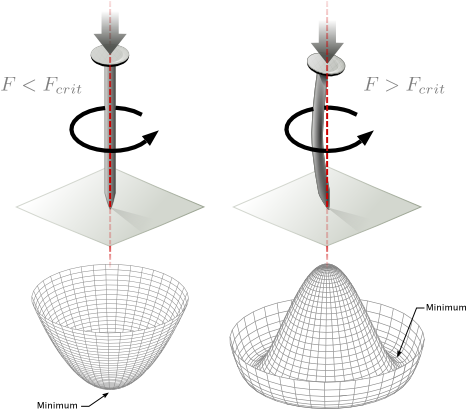
\includegraphics[scale=0.4]{broken_symmetry}
\caption[Spontaneous symmetry breaking mechanism]{Spontaneous symmetry breaking mechanism. The steel nail, subject to an external force (top left), has rotational symmetry with respect to its axis. When the external force overcomes a critical value the nail buckles (top right) choosing a minimal energy state (ground state) and thus \textit{``breaking spontoaneously the rotational symmetry''}. The potential energy (bottom) changes but holds the rotational symmetry; however, an infinite number of asymmetric ground states are generated and circularly distributed in the bottom of the potential\cite{broken_symmetry}.}
\label{ssb}
\end{figure}

Before reaching the critical force value, the system has rotational symmetry with respect to the nail axis; however, after the critical force value is reached the nail buckles (top right). The form of the potential energy (bottom right) changes, preserving its rotational symmetry although its minima does not exhibit that rotational symmetry any longer. Right before the nail buckles there is no indication of the direction the nail will bend because any of the directions are equivalent, but once the nail bends, choosing a direction, an arbitrary minimal energy state (ground state) is selected and it does not share the system's rotational symmetry. This mechanism for reaching an asymmetric ground state is known as \textit{``spontaneous symmetry breaking''}.       

The lesson from this analysis is that the way to introduce the SSB mechanism into a system is by adding the appropriate potential to it.\\ 

Figure \ref{hp2d} shows a plot of the potential $V(\phi)$ in the case of a scalar field $\phi$

\beqn\label{Higgs_potential}
V(\phi)=\mu^2\phi^\dagger\phi + \lambda(\phi^\dagger\phi)^2
\eeqn

If $\mu^2>0$ the potential has only one minimum at $\phi=0$ and describes a scalar field with mass $\mu$. If $\mu^2<0$ the potential has a local maximum at $\phi=0$ and two minima at $\phi=\pm \sqrt{-\mu^2/\lambda}$ which enables the SSB mechanism to work.\\ 

\begin{figure}[!h]
\centering
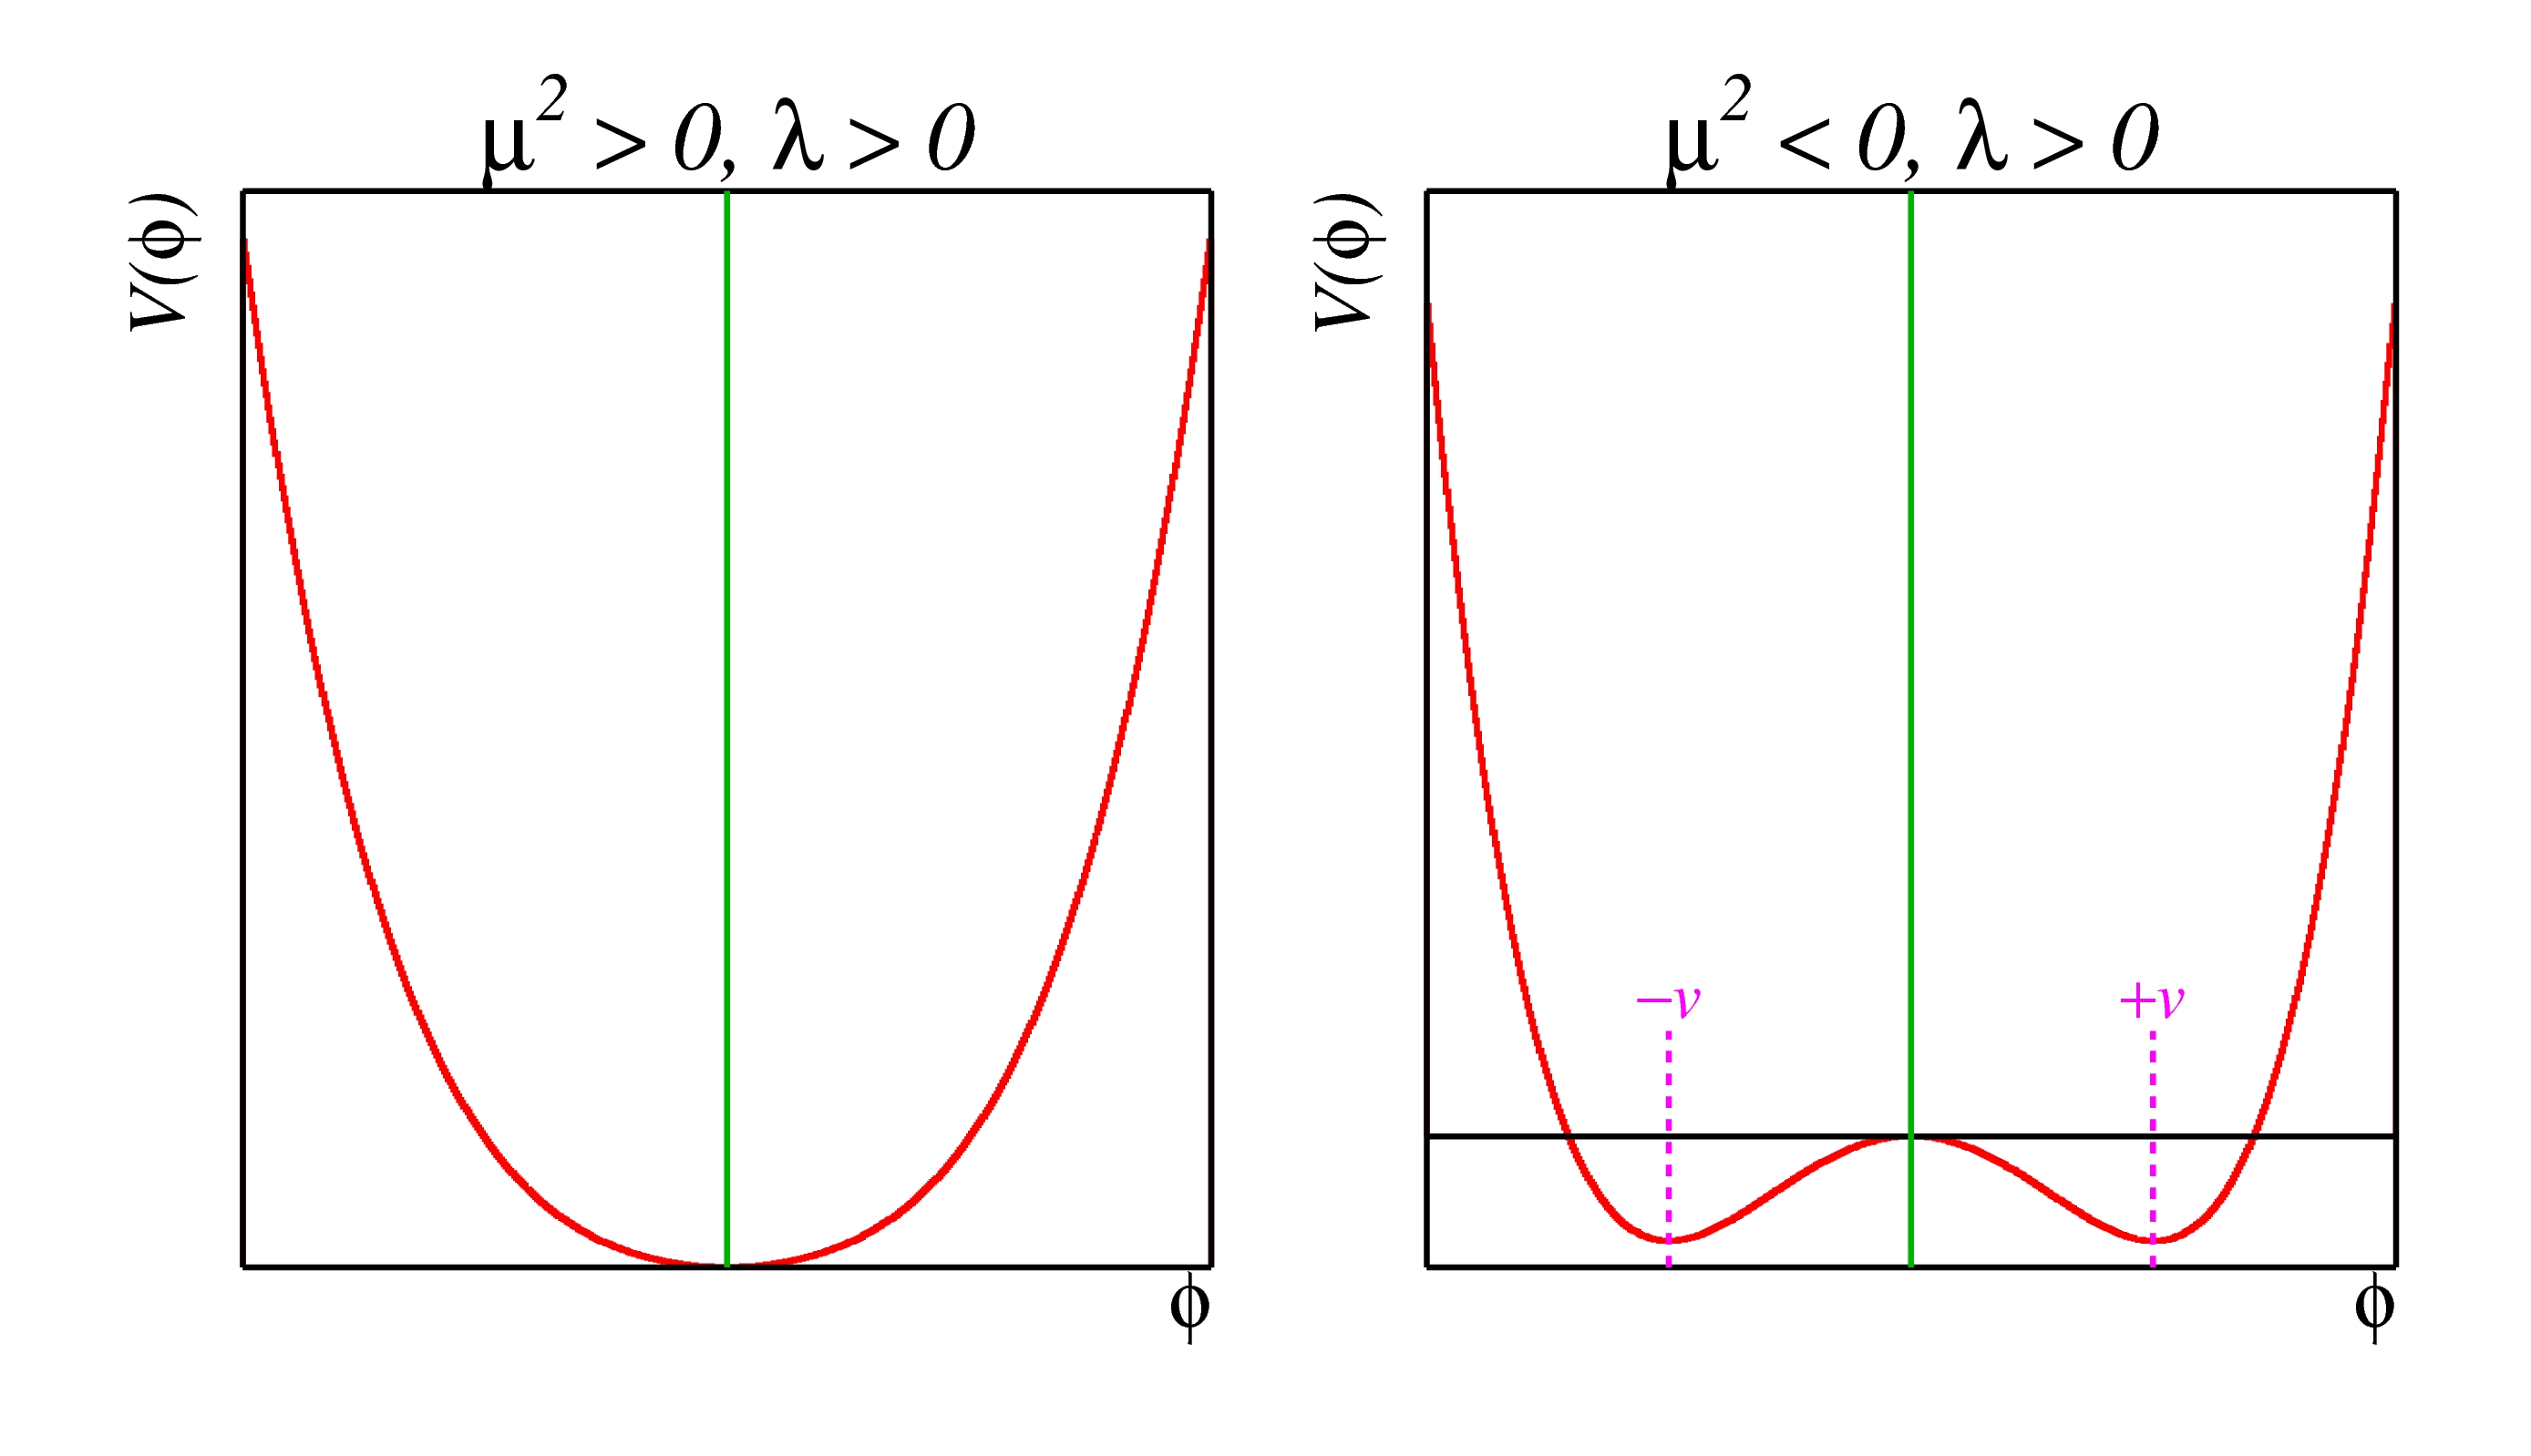
\includegraphics[scale=0.4]{hp2d}
\caption[SSB Potential form]{Shape of the potential $V(\phi)$ for $\lambda>0$ and: $\mu^2>0$ (left) and $\mu^2<0$ (right). The case $\mu^2<0$ corresponds to the potential suitable for introducing the SSB mechanism by choosing one of the two ground states which are connected via refletion symmetry. \cite{broken_symmetry}.}
\label{hp2d}
\end{figure}

In the case of a complex scalar field $\phi(x)$

\beqn\label{complex_scalar}
\phi(x)=\frac{1}{\sqrt{2}}(\phi_1 + i \phi_2)
\eeqn
\noindent the Lagrangian (invariant under global $U(1)$ transformations) is given by 
\beqn\label{higgs_potential}
\Lagr=(\partial_\mu\phi)^\dagger(\partial^\mu\phi) - V(\phi) , \qquad V(\phi)=\mu^2\phi^\dagger\phi + \lambda(\phi^\dagger\phi)^2
\eeqn

\noindent where an appropiate potential has been added in order to introduce the SSB.\\

As seen in Figure \ref{higgs_potential_plot}, the potential has now an infinite number of minima circularly distributed along the $\xi$-direction which makes possible the occurence of the SSB by choosing an arbitrary ground state; for instance, $\xi=0$, \ie $\phi_1=v, \phi_2=0$

\begin{figure}[!h]
\centering
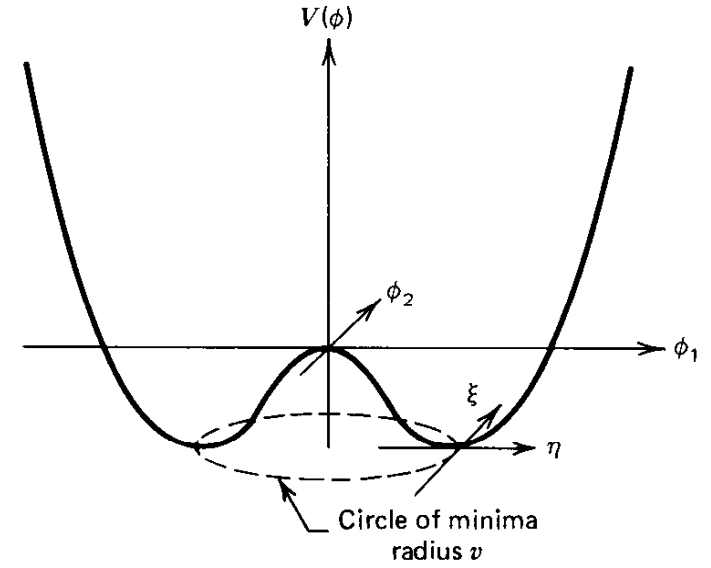
\includegraphics[scale=0.3]{higgs_potential_plot}
\caption[Potential for complex scalar field ]{Potential for complex scalar field. There is a circle of minima of radius \textit{v} along the $\xi$-direction\cite{halzen}.}
\label{higgs_potential_plot}
\end{figure}

\beqn
\phi_0=\frac{v}{\sqrt{2}}\exp(i\xi) \quad \xrightarrow[]{SSB} \quad \phi_0=\frac{v}{\sqrt{2}}
\eeqn

As usual, excitations over the ground state are studied by making an expansion about it; thus, the excitation can be parametrized as:
\beqn
\phi(x)=\frac{1}{\sqrt{2}}(v + \eta(x) + i\xi(x))
\eeqn

\noindent which when substituted into eqn. \ref{higgs_potential} produces a Lagrangian in terms of the new fields $\eta$ and $\xi$

\beqn\label{lagr_complex_field}
\Lagr'=\frac{1}{2}(\partial_\mu\xi)^2 + \frac{1}{2}(\partial_\mu\eta)^2 + \mu^2\eta^2 - V(\phi_0) - \lambda v \eta(\eta^2+\xi^2) -  \frac{\lambda}{4}(\eta^2+\xi^2)^2
\eeqn

\noindent where the last two terms represent the interactions and self-interaction between the two fields $\eta$ and $\xi$. The particular feature of the SSB mechanism is revealed when looking to the first three  terms of $\Lagr'$. Before the SSB, only the massless $\phi$ field is present in the system; after the SSB there are two fields of which the $\eta$-field has acquired mass $m_\eta=\sqrt{-2\mu^2}$ while the $\xi-field$ is still massless (see Figure \ref{higgs_hat}).\\  

\begin{figure}[!h]
\centering
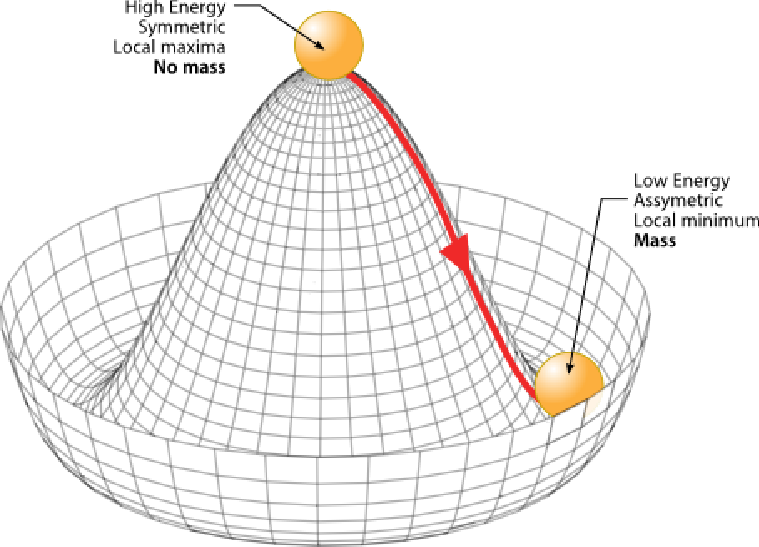
\includegraphics[width=0.48\textwidth]{higgs_hat}
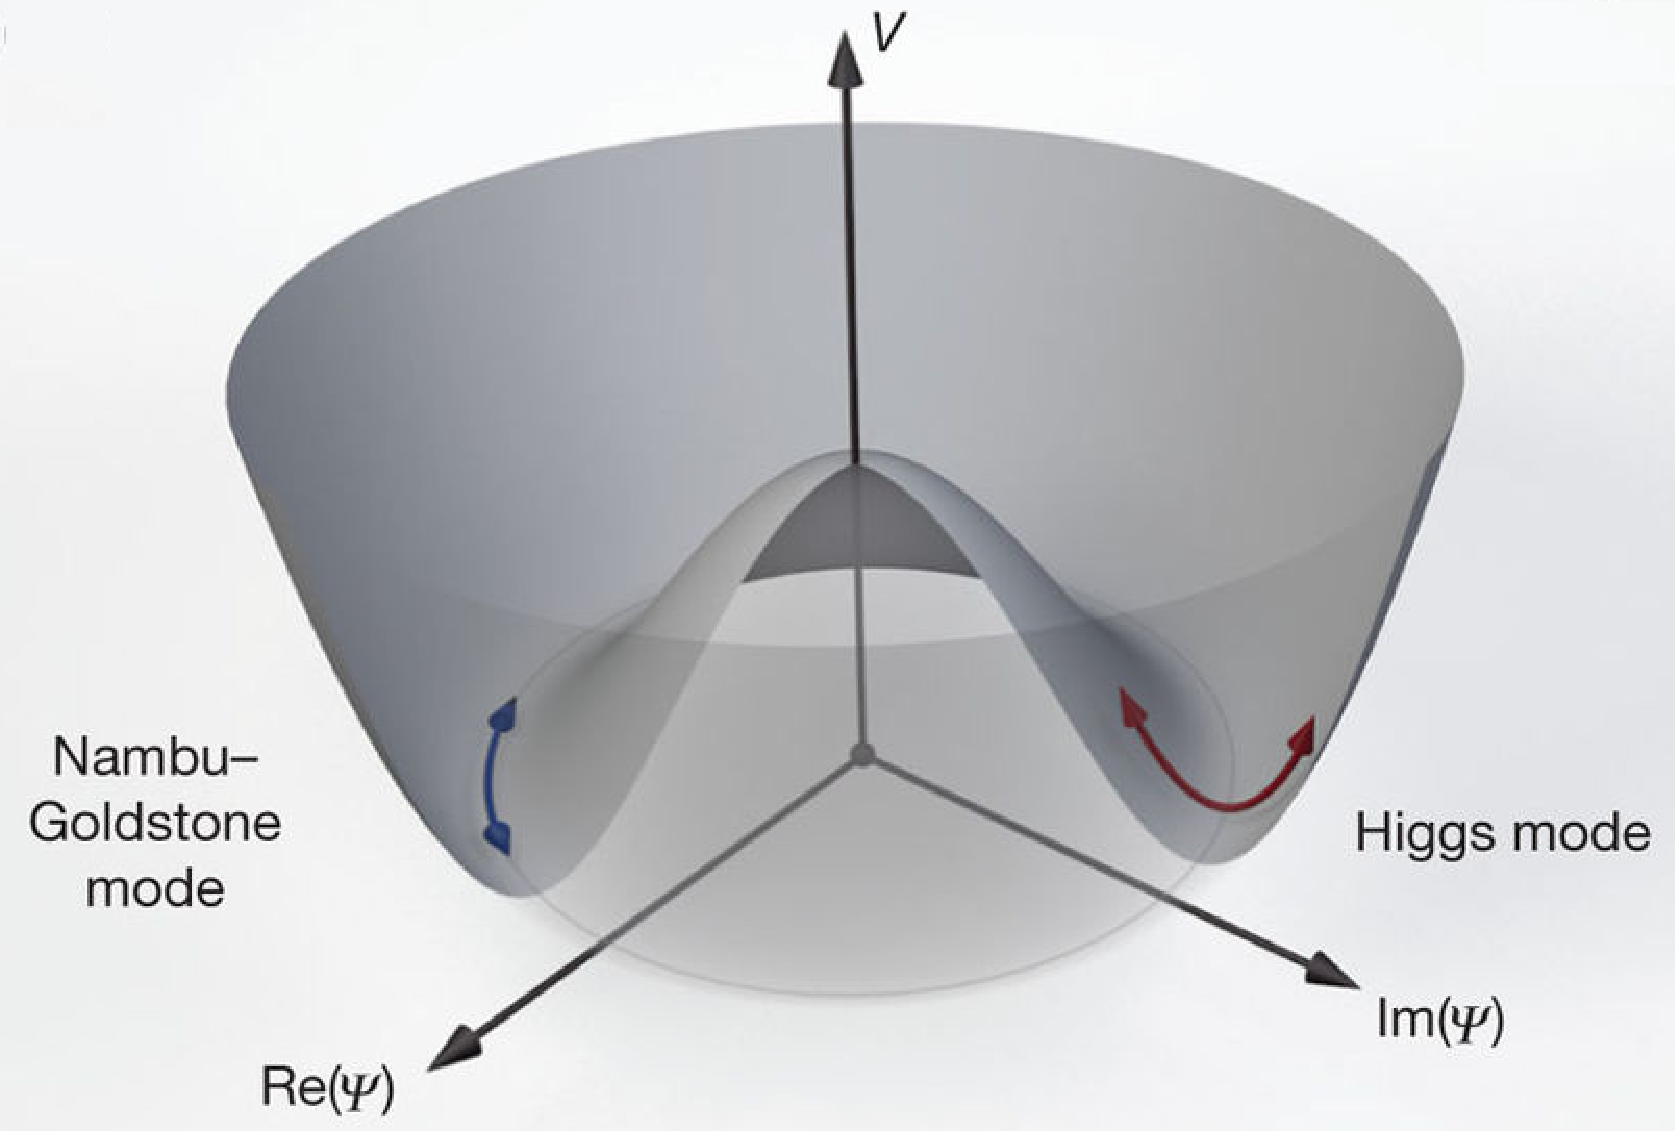
\includegraphics[width=0.5\textwidth]{goldstone_boson_mode}
\caption[SSB mechanism for complex scalar field]{SSB mechanism for a complex scalar field\cite{broken_symmetry,endres}.}
\label{higgs_hat}
\end{figure}

Thus, \textit {the SSB mechanism serves as a method to generate mass but as a side effect a massless field is introduced in the system}. This fact is known as the Goldstone theorem and states that a massless scalar field appears in the system for each continuous symmetry spontaneously broken. Another version of the Goldstone theorem states that \textit{``if a Lagrangian is invariant under a continuous symmetry group G, but the vacuum is only invariant under a subgroup $H\subset G$, then there must exist as many massless spin-0 particles (Nambu-Goldstone bosons) as broken generators.''}\cite{pich} The Nambu-Goldstone boson can be understood considering that the potential in the $\xi$-direction is flat so excitations in that direction are not energy consuming and thus represent a massless state.                   

\subsection{Higgs mechanism}

\noindent When the SSB mechanism is introduced in the formulation of the EWI in an attempt to generate the mass of the so far massless gauge bosons and fermions, an interesting effect is revealed. In order to keep the G symmetry group invariance and generate the mass of the EW gauge bosons, a G invariant Lagrangian density ($\Lagr_S$) has to be added to the non massive EWI Lagrangian (eqn. \ref{nmewi_lagr})

\begin{align}
\Lagr_S    = &(D_\mu\phi)^\dagger(D^\mu\phi) - \mu^2\phi^\dagger\phi - \lambda(\phi^\dagger\phi)^2 , \qquad \lambda>0, \mu^2<0 \label{ls}\\
D_\mu\phi = &\left(i\partial_\mu - g\frac{\sigma_i}{2}W^i_\mu -
g'\frac{Y}{2}B_\mu\right)\phi
\end{align}

\noindent $\phi$ has to be an isospin doublet of complex scalar fields so it preserves the G invariance; thus $\phi$ can be defined as:

\beqn
\phi = \binom{\phi^+}{\phi^0} \equiv \frac{1}{\sqrt{2}}\binom{\phi_1 + i\phi_2}{\phi_3 + i\phi_4}.
\eeqn

The minima of the potential are defined by

\beqn
\phi^\dagger\phi=\frac{1}{2}(\phi_1^2 +\phi_2^2 +\phi_3^2 + \phi_1^4 )= -\frac{\mu^2}{2\lambda}.
\eeqn

The choice of the ground state is critical. By choosing a ground state, invariant under $U(1)_{em}$ gauge symmetry, the photon will remain massless and the $\wpm$ and $Z$ bosons masses will be generated which is exactly what is needed. In that sense, the best choice corresponds to a weak isospin doublet with $T_3=-1/2$, $Y_W=1$ and $Q=0$ which defines a ground state with $\phi_1=\phi_2=\phi_4$ and $\phi_3=v$:

\beqn\label{field_exp}
\phi_0\equiv\frac{1}{\sqrt{2}}\binom{0}{v}, \qquad v^2\equiv-\frac{\mu^2}{\lambda}.
\eeqn

\noindent where the vacuum expectation value $v$ is fixed by the Fermi coupling $G_F$ according to $v=(\sqrt{2}G_F)^{1/2}\approx 246$ GeV.\\

The G symmetry has been broken and three Nambu-Goldstone bosons will appear. The next step is to expand $\phi$ about the chosen ground state as:
\beqn
\phi(x) = \frac{1}{\sqrt{2}}\exp\left(\frac{i}{v}\sigma_i\theta^i(x)\right) \binom{0}{v+H(x)}\approx \frac{1}{\sqrt{2}}\binom{\theta_1(x) + i\theta_2(x)}{v + H(x) - i\theta_3(x)} 
\eeqn

\noindent to describe fluctuations from the ground state $\phi_0$. The fields $\theta_i(x)$ represent the Nambu-Goldstone bosons while $H(x)$ is known as ``higgs field.'' The fundamental feature of the parametrization used is that the dependence on the $\theta_i(x)$ fields is factored out in a global phase that can be eliminated by taking the physical ``unitary gauge'' $\theta_i(x)=0$. Therefore the expansion about the ground state is given by:
\beqn\label{higgs_dublet}
\phi(x)\frac{1}{\sqrt{2}}\binom{0}{v+H(x)}
\eeqn

\noindent which when substituted into $\Lagr_S$ (eqn. \ref{ls}) results in a Lagrangian containing the now massive three gauge bosons $\wpm, Z$, one massless gauge boson (photon) and the new Higgs field (H). The three degrees of freedom corresponding to the Nambu-Goldstone bosons are now integrated into the massive gauge bosons as their longitudinal polarizations which were not available when they were massless particles. The effect by which vector boson fields acquire mass after an spontaneous symmetry breaking, but without an explicit gauge invariance breaking is known as the \textit{``Higgs mechanism''}.\\

The mechanism was proposed by three independent groups: F.Englert and R.Brout in August 1964 \cite{englert}, P.Higgs in October 1964 \cite{higgs} and G.Guralnik, C.Hagen and T.Kibble in November 1964\cite{ghk}; however, its importance was not realized until S.Glashow\cite{glashow}, A.Salam\cite{salam} and S.Weinberg \cite{weinberg}, independently, proposed that electromagnetic and weak interactions are two manifestations of a more general interaction called ``electroweak interaction'' in 1967.

\subsection{Masses of the gauge bosons}

The mass of the gauge bosons is extracted by evaluating the kinetic part of Lagrangian $\Lagr_S$ in the ground state (known also as the vacuum expectation value), \ie,

\beqn\label{gauge_masses}
\small
\left|\left(\partial_\mu - ig\frac{\sigma_i}{2}W^i_\mu -i\frac{g'}{2}B_\mu\right)\phi_0\right |^2= \left(\frac{1}{2}vg\right)^2W_\mu^+W^{-\mu} + \frac{1}{8}v^2(W_\mu^3,B_\mu)\binom{g^2 \quad -gg'}{-gg' \quad g'^2}\binom{W^{3\mu}}{B^\mu}
\eeqn

\noindent comparing with the typical mass term for a charged boson $M_W^2 W^+W^-$
\beqn
M_W=\frac{1}{2}vg.
\eeqn
The second term in the right side of the eqn.\ref{gauge_masses} comprises the masses of the neutral bosons, but it needs to be written in terms of the gauge fields $Z_\mu$ and $A_\mu$ in order to be compared to the typical mass terms for neutral bosons, therefore using eqn. \ref{neutral_bosons}
\begin{align}
\frac{1}{8}v^2[g^2(W_\mu^3)^2-2gg'W_\mu^3B^\mu + g'^2B_\mu^2]=&\frac{1}{8}v^2[ g W^3_\mu - g'B_\mu]^2 + 0[g'W^3_\mu + gB_\mu]^2\\
                                                             =&\frac{1}{8}v^2[\sqrt{g^2+g'^2}Z_\mu]^2 + 0[\sqrt{g^2+g'^2}A_\mu]^2\nonumber                                                             
\end{align}

\noindent and then

\beqn
M_Z= \frac{1}{2}v\sqrt{g^2+g'^2}, \qquad M_A=0 
\eeqn

\subsection{Masses of the fermions}
The lepton mass terms can be generated by introducing a gauge invariant Lagrangian term describing the Yukawa coupling between the lepton field and the Higgs field
\beqn\label{lyl}
\Lagr_{Yl}=-G_l\left[(\bar{\nu_l}, \bar{l})_L\binom{\phi^+}{\phi^0}l_R + \bar{l}_R(\phi^-,\bar{\phi}^0)\binom{\nu_l}{l}_L\right], \qquad l=e,\mu,\tau.
\eeqn

 After the SSB and replacing the usual field expansion about the ground state (eqn.\ref{field_exp}) into $\Lagr_{Yl}$, the mass term arises
\beqn\label{lyl2}
\Lagr_{Yl}=-m_l(\bar{l}_Ll_R + \bar{l}_R{l}_L) -\frac{m_l}{v}(\bar{l}_Ll_R + \bar{l}_R{l}_L)H= -m_l \bar{l}l\left(1+ \frac{H}{v}\right)                   
\eeqn
\beqn
m_l=\frac{G_l}{\sqrt{2}}v
\eeqn
\noindent where the additional term represents the lepton-Higgs interaction. The quark masses are generated in a similar way as lepton masses but for the upper member of the quark doublet a different Higgs doublet is needed:
\beqn
\phi_c=-i\sigma_2\phi* = \binom{-\bar{\phi}^0}{\phi^-}.
\eeqn
Additionally, given that the quark isospin doublets are not constructed in terms of the mass eigenstates but in terms of the flavor eigenstates, as shown in Table\ref{T3Y}, the coupling parameters will be related to the CKM matrix elements; thus the quark Lagrangian is given by:   

\beqn\label{lyq}
\Lagr_{Yq}=-G_d^{i,j}(\bar{u_i},\bar{d'_i})_L\binom{\phi^+}{\phi^0}d_{jR} - G_u^{i,j}(\bar{u_i},\bar{d'_i})_L\binom{-\bar{\phi^0}}{\phi^-}u_{jR} + h.c. 
\eeqn

\noindent with i,j=1,2,3. After SSB and expansion about the ground state, tha diagonal form of $\Lagr_{Yq}$ is:
\beqn\label{lyq2}
\Lagr_{Yq}=-m_d^i\bar{d_i}d_i\left(1 +\frac{H}{v}\right) - m_u^i\bar{u_i}u_i\left(1 +\frac{H}{v}\right)
\eeqn

Fermion masses depend on arbitrary couplings $G_l$ and $G_{u,d}$ and are not predicted by the theory.  

\subsection{The Higgs field}

After the characterization of the fermions and gauge bosons as well as their interactions, it is necessary to characterize the Higgs field itself. The Lagrangian $\Lagr_S$ in eqn. \ref{ls} written in terms of the gauge bosons is given by
\beqn
\Lagr_S= \frac{1}{4}\lambda v^4 + \Lagr_H +\Lagr_{HV}
\eeqn
\beqn\label{lh}
\Lagr_H= \frac{1}{2}\partial_\mu H\partial^\mu H -  \frac{1}{2}m_H^2 H^2 - \frac{1}{2v}m_H^2 H^3 -  \frac{1}{8v^2}m_H^2 H^4
\eeqn
\beqn\label{lhV}
\Lagr_{HV}= m_H^2W_\mu^+W^{\mu-}\left(1+ \frac{2}{v}H +  \frac{2}{v^2}H^2 \right) + \frac{1}{2}m_Z^2Z_\mu Z^\mu\left(1+ \frac{2}{v}H +  \frac{2}{v^2}H^2 \right) 
\eeqn
The mass of the Higgs boson is deduced as usual from the mass term in the Lagrangian resulting in:
\beqn
m_H=\sqrt{-2\mu^2}=\sqrt{2\lambda}v
\eeqn
\noindent however, it is not predicted by the theory either. The experimental efforts to find the Higgs boson, carried out by the ``Compact Muon Solenoid (CMS)'' experiment and the ``A Toroidal LHC AppartuS (ATLAS)'' experiments at the ``Large Hadron Collider(LHC)'', gave great results by July of 2012 when the discovery of a new particle compatible with the Higgs boson predicted by the electroweak theory\cite{hcms,hatlas} was announced. Although at the announcement time there were some reservations about calling the new particle the ``Higgs boson'', today this name is widely accepted. The Higgs mass measurement, reported by both experiments\cite{hmass}, is in Table \ref{higgs_prop}. 
\begin{center}
\begin{table}[h]
\centering
\scriptsize
\begin{tabular}{lc}\hline
Property         & Value  \\ \hline
Electric charge  & 0      \\
Colour charge    & 0      \\
Spin             & 0      \\
Weak isospin     & -1/2    \\
Weak hypercharge & 1      \\
Parity           & 1      \\\hline
Mass (GeV/c$^2$) & 125.09$\pm$0.21 (stat.)$\pm$0.11 (syst.)\\\hline
\end{tabular}
\caption[Higgs boson properties.]{Higgs boson properties. Higgs mass is not predicted by the theory and the value here corresponds to the experimental measurement.}\label{higgs_prop}
\end{table}
\end{center}

\subsection{Production of Higgs bosons at LHC}

At LHC, Higgs boson is produced as a result of the collision of two counter-rotating protons beams. A detailled description of the LHC machine will be presented in chapter \ref{ch:cms}. ``The total cross section'' is a parameter that quantifies the number of pp collisions that happen when a number of protons are fired at each other. Different results can be obtained after a pp collision and for each one the ``cross section'' is defined as the number of pp collisions that conclude in that particular result with respect to the number of protons fired at each other.
\begin{figure}[!h]
\centering
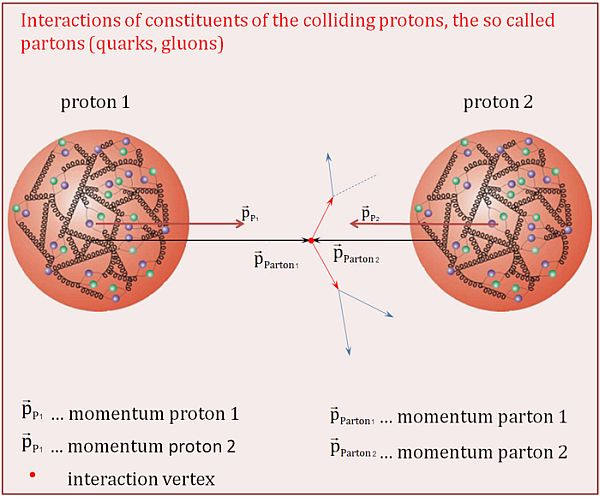
\includegraphics[scale=0.55]{proton_proton}
\caption[Proton-Proton collision]{Proton-proton collision. Protons are composed of 3 valence quarks, a sea of quarks and gluons; therefore in a proton-proton collision, quarks and gluons are those who collide. \cite{pp_coll}.}
\label{pp_collision}
\end{figure}

Protons are composed of quarks and these quarks are bound by gluons; however, what is commonly called the quark content of the proton makes reference to the valence quarks. A sea of quarks and gluons is also present inside the proton as represented in Figure \ref{pp_collision}. In a proton-proton (pp) collision, the constituents (quarks and gluons) are those who collide. The pp cross section depends on the momentum of the colliding particles, reason for which it is needed to know how the momentum is distributed inside the proton. Quarks and gluons are known as partons and the functions that describe how the proton momentum is distributed among partons inside it are called ``parton distribution functions (PDFs)''; PDFs are determined from experimental data obtanied in experiments where the internal structure of hadrons is tested.\\

In addition, in physics, a common approach to study complex systems consists in starting with a simpler version of them, for which a well known description is available, and add an additional ``perturbation'' which represents a small deviation from the known behavior. If the perturbation is small enough, the physical quanties associated with the perturbed system are expressed as a series of corrections to those of the simpler system; therefore, the more terms are considered in the series (the higher order in the perturbation series), the more precise is the the description of the complex system.\\

This thesis explores the Higgs production at LHC; therefore the overview presented here will be oriented specifically to the production mechanisms after pp collisions at LHC.

\begin{figure}[!h]
\centering
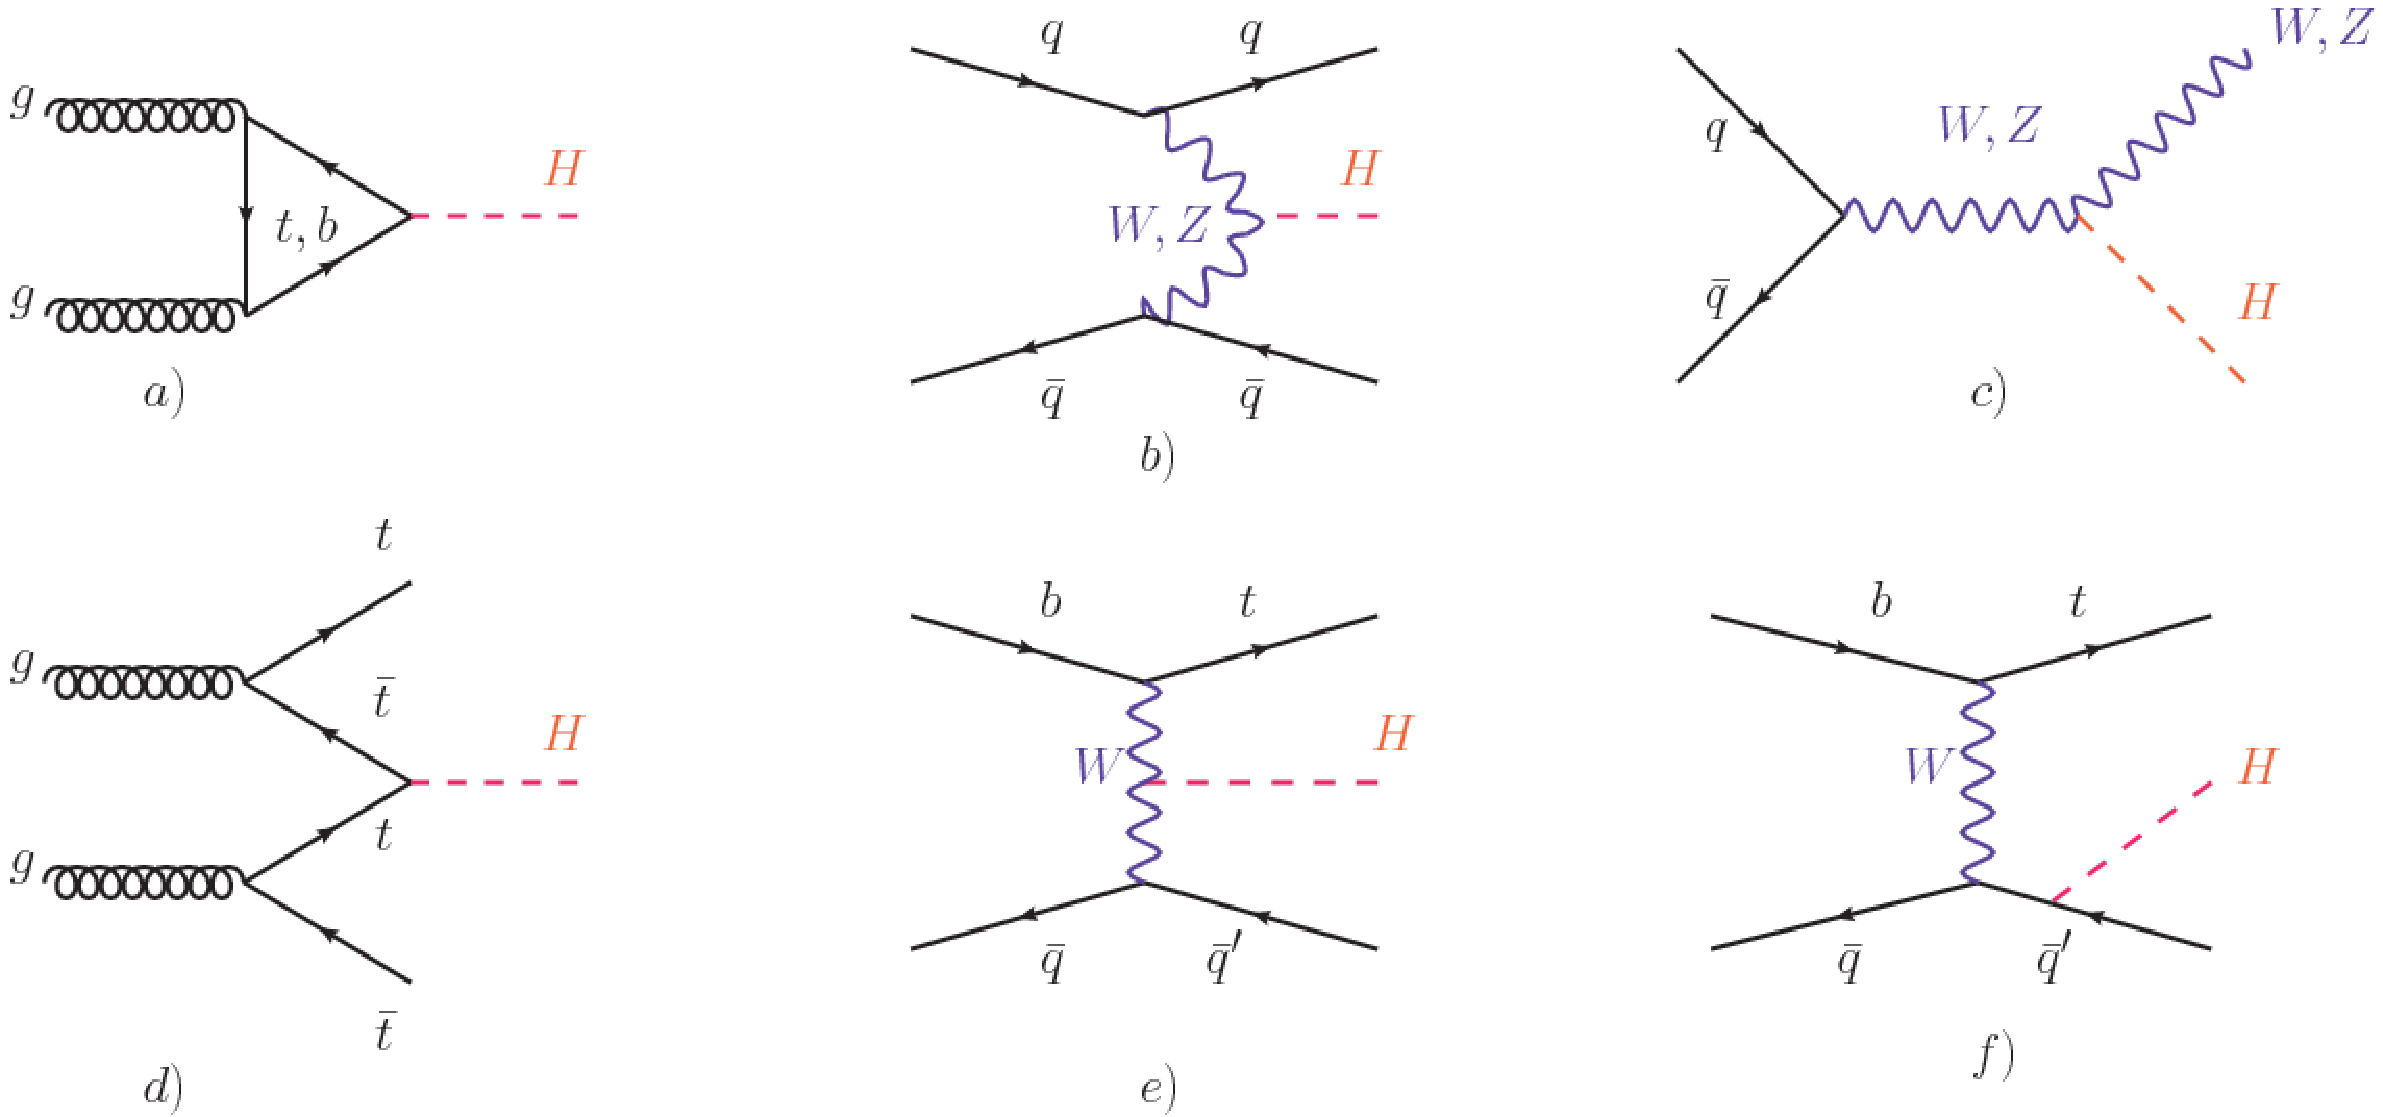
\includegraphics[scale=0.3]{higgs_prod}
\caption[Higgs boson production mechanism Feynman diagrams]{Main Higgs boson production mechanism Feynman diagrams. a. gluon-gluon fusion, b. vector boson fusion (VBF), c. Higgs-strahlung, d. Associated production with a top or bottom quark pair, e-f. associated production with a single top quark.}
\label{higgs_prod}
\end{figure}

Figure \ref{higgs_prod} shows the Feynman diagrams for the leading order (first order) Higgs production processes at LHC, while the cross section for Higgs production as a function of the center of mass-energy ($\sqrt{s}$) for pp collisions is showed in Figure \ref{hcs_br} left. The tags NLO (next to leading order), NNLO (next to next to leading order) and N3LO (next to next to next to leading order) make reference to the order at which the pertubation series have been considered.
%% Table \ref{hxsec} present the cross sections for $m_H=125GeV/c^2$.
%% \begin{center}
%% \begin{table}[h]
%% \centering
%% \begin{tabular}{lllllll}\hline
%% $\sqrt{s}$(TeV) &\multicolumn{6}{l}{Production cross section (in pb) for $m_H$ = 125 GeV/c$^2$}\\\hline
%%                 & ggF          & VBF          & WH           & ZH           & $t\bar{t}H$           & total \\\hline
%% 7               & $16.9\pm5\%$ & $1.24\pm2\%$ & $0.58\pm3\%$ & $0.34\pm4\%$ & $0.09^{+8\%}_{-14\%}$ & 19.1  \\
%% 8               & $21.4\pm5\%$ & $1.60\pm2\%$ & $0.70\pm3\%$ & $0.42\pm5\%$ & $0.13^{+8\%}_{-13\%}$ & 24.2  \\
%% 13              & $48.6\pm5\%$ & $3.78\pm2\%$ & $1.37\pm2\%$ & $0.88\pm5\%$ & $0.50^{+9\%}_{-13\%}$ & 55.1  \\
%% 14              & $54.7\pm5\%$ & $4.28\pm2\%$ & $1.51\pm2\%$ & $0.99\pm5\%$ & $0.60^{+9\%}_{-13\%}$ & 62.1  \\\hline
%% \end{tabular}
%% \caption[The SM Higgs boson production cross sections for $m_H = 125 GeV/c^2$.]{The SM Higgs boson production cross sections for $m_H = 125 GeV/c^2$.in pp collisions as a function of
%% the center of mass energy, $\sqrt{s}$. The predictions for the ggF channel at the LHC include the latest N3LO results leading to reduced theoretical uncertainties by a factor around 2 compared to the N2LO results.\cite{pdg}}\label{hxsec}
%% \end{table}
%% \end{center}

\begin{figure}[!h]
\centering
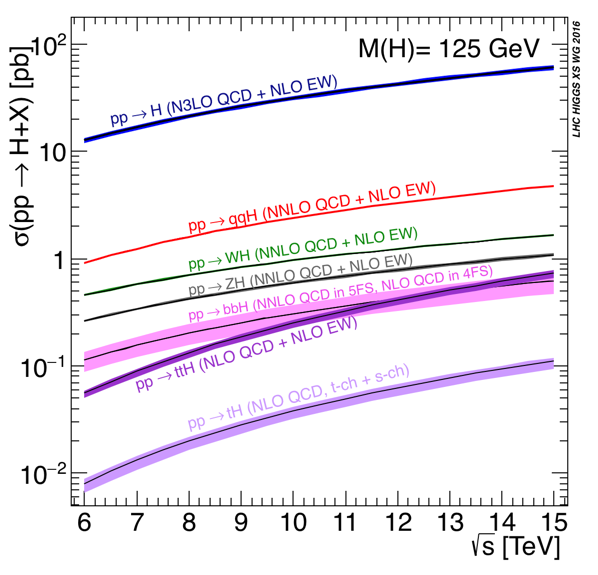
\includegraphics[width=0.40\textwidth]{higgs_prod_plot}
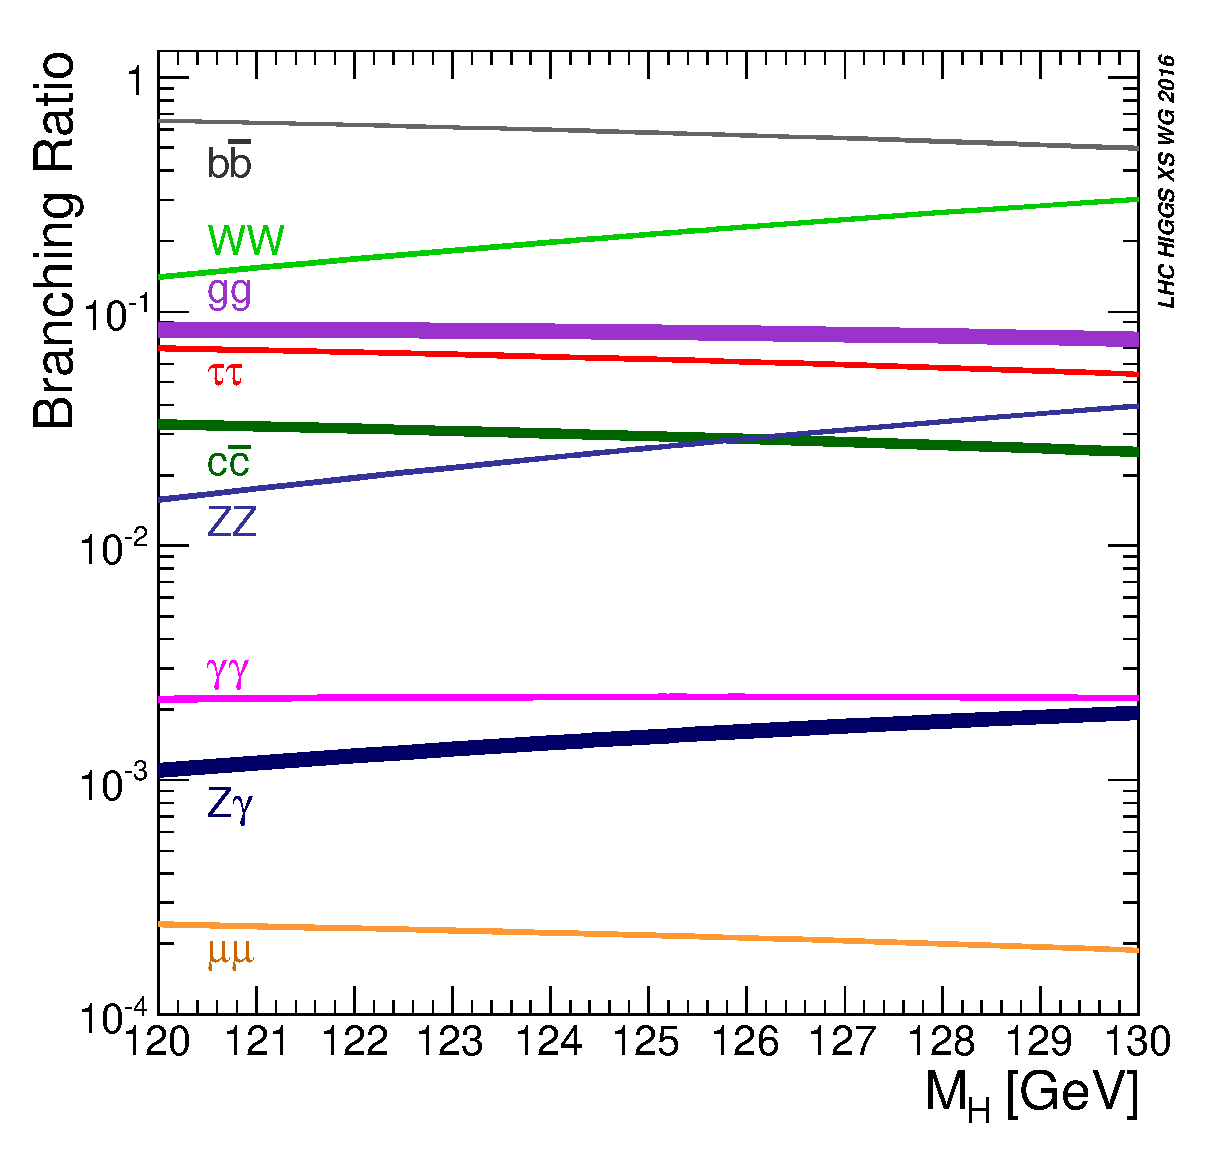
\includegraphics[width=0.40\textwidth]{higgsbr}
\caption[Higgs boson production cross section and decay branching ratios]{Higgs boson production cross sections (left) and decay branching ratios (right) for the main mechanisms. The VBF is indicated as qqH\cite{hcswg}.}
\label{hcs_br}
\end{figure}

As shown in eqns \ref{lyl}, \ref{lyq} and \ref{lhV}, the strength of the Higgs-fermion interaction is proportional to the fermion mass while the strength of the Higgs-gauge boson interaction is proportional to the square of the gauge boson mass, which implies that the Higgs production and decay mechanisms are dominated by couplings $H-(W,Z,t,b,\tau)$. 

The main production mechanism is the gluon fusion (Figure \ref{higgs_prod}a and $pp\to H$ in Figure \ref{hcs_br}) given that gluons carry the highest fraction of momentum of the protons in pp colliders. Since the Higgs boson does not couple to gluons, the mechanism proceeds through the exchange of a virtual top-quark loop given that for it the coupling is the biggest. Note that in this process, the Higgs boson is produced alone, which makes this mechanism experimentally clean when combined with the two-photon or the four-lepton decay channels (see Section \ref{sec:decays}).

Vector boson fusion (Figure \ref{higgs_prod}b and $pp\to qqH$ in Figure \ref{hcs_br}) has the second largest production cross section. The scattering of two fermions is mediated by a weak gauge boson which later emits a Higgs boson. In the final state, the two fermions tend to be located in a particular region of the detector which is used as a signature when analyzing the datasets provided by the experiments. More details about how to identify events of interest in an analysis will be given in chapter \ref{ch:analysis}. 

The next production mechanism is Higgs-strahlung (Figure \ref{higgs_prod}c and $pp\to WH, pp\to ZH$ in Figure \ref{hcs_br}) where two fermions annihilate to form a weak gauge boson. If the initial fermions have enough energy, the emergent boson eventually will emit a Higgs boson.

The associated production with a top or bottom quark pair and the associated production with a single top quark (Figure \ref{higgs_prod}d-f and $pp\to bbH, pp\to \ttH, pp\to tH$ in Figure \ref{hcs_br}) have a smaller cross section than the main three mechanisms above, but they provide a good opportunity to test the Higgs-top coupling. The analysis reported in this thesis is developed using these production mechanisms. A detailed description of the \tH mechanism will be given in Section \ref{sec:thq}.  

\subsection{Higgs boson decay channels}\label{sec:decays}

When a particle can decay throught several modes, also known as channels, the probability of decaying throught a given channel is quantified by the ``branching ratio (BR)'' of the decay channel; thus, the BR is defined as the ratio of number of decays going throught that given channel to the total number of decays. In regard to the Higgs boson decay, the BR can be predicted with accuracy once the Higgs mass is known \cite{riley, denner}. In Figure \ref{hcs_br} right, a plot of the BR as a function of the Higgs mass is presented. The largest predicted BR corresponds to the $b\bar{b}$ pair decay channel (see Table \ref{hdbr}). %In this thesis the $H \to WW$ channel will be considered.        

\begin{center}
\begin{table}[h]
\centering
\begin{tabular}{lll}\hline
Decay channel       & Branching ratio   & Rel. uncertainty\\\hline
$H\to b\bar{b}$     & $5.84\times10^-1$ & $+3.2\%-3.3\%$\\
$H\to W^+W^-$       & $2.14\times10^-1$ & $+4.3\%-4.2\%$\\
$H\to\tau^+\tau^-$  & $6.27\times10^-2$ & $+5.7\%-5.7\%$\\
$H\to ZZ$           & $2.62\times10^-2$ & $+4.3\%-4.1\%$\\
$H\to \gamma\gamma$ & $2.27\times10^-3$ & $+5.0\%-4.9\%$\\
$H\to Z\gamma$      & $1.53\times10^-3$ & $+9.0\%-8.9\%$\\
$H\to\mu^+\mu^-$    & $2.18\times10^-4$ & $+6.0\%-5.9\%$\\\hline
\end{tabular}
\caption[Predicted branching ratios for a SM Higgs boson with $m_H = 125$ GeV/c$^2$.]{Predicted branching ratios and the relative uncertainty for a SM Higgs boson with $m_H = 125GeV/c^2$.\cite{pdg}}\label{hdbr}
\end{table}
\end{center}
%______________________ tHq ______________________
\section{Associated production of a Higgs boson and a single Top quark.}\label{sec:thq}

\begin{figure}[h!]
\centering
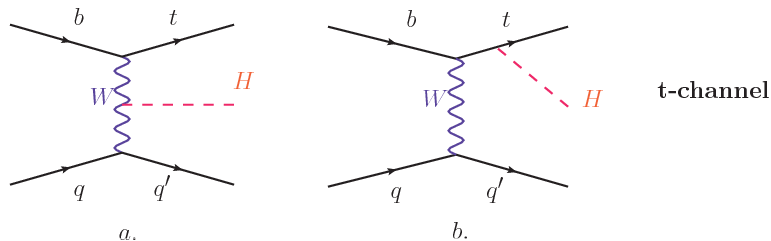
\includegraphics[scale=0.4]{thq_prod}\\
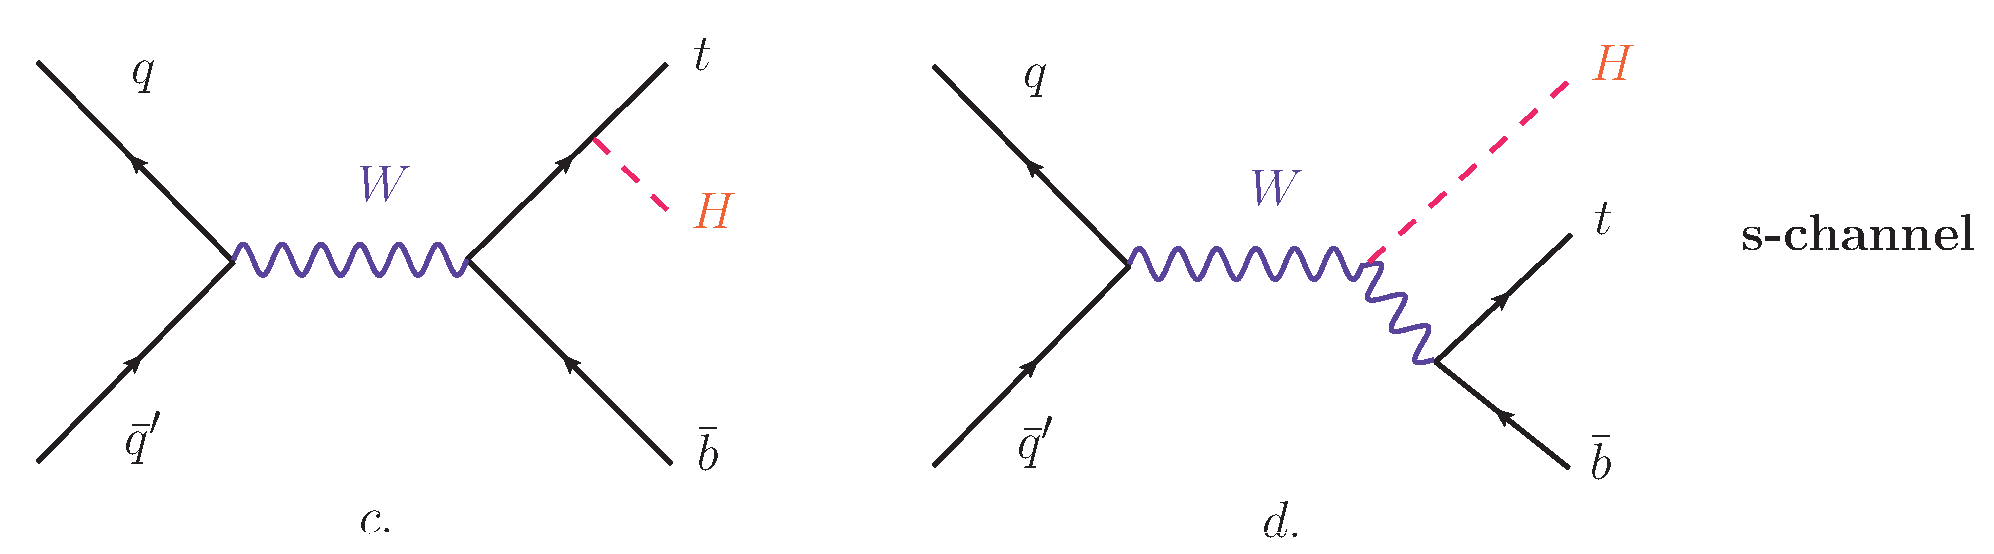
\includegraphics[scale=0.4]{thb_prod}\\
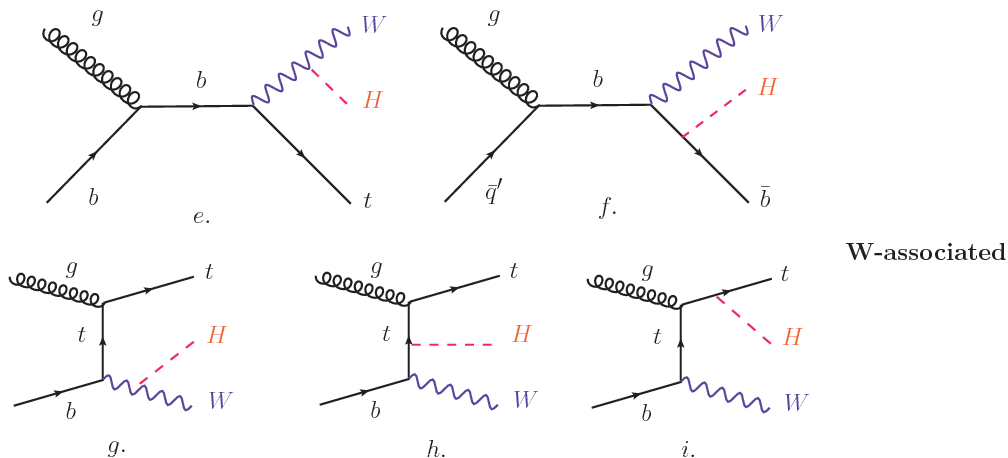
\includegraphics[scale=0.4]{thW_prod}\\
\caption[Associated Higgs boson production mechanism Feynman diagrams]{Associated Higgs boson production mechanism Feynman diagrams. a.,b. t-channel (tHq), c.,d. s-channel (tHb), e-i. W-associated.}
\label{fig:th_prod}
\end{figure}

Associated production of Higgs boson has been extensively studied \cite{maltoni1, biswas, farina,tait, maltoni2}. While measurements of the main Higgs production mechanisms rates are sensitive to the strength of the Higgs coupling to W boson or top quark, they are not sensitive to the relative sign between the two couplings. In this thesis, the Higgs boson production mechanism explored is the associated production with a single top quark (\tH) which offers sensitiveness to the relative sign of the Higgs couplings to W boson and to top quark. The description given here is based on the Reference \cite{farina}\\

A process where two incoming particles interact and produce a final state with two particles can proceed in three ways also called channels (see, for instance, Figure \ref{fig:th_prod} ommiting the red line). The t-channel represents processes where an intermediate particle is emited by one of the incoming particles and absorbed by the other. The s-channel represents processes where the two incoming particles merge into an intermediate particle which eventually will split into the particles in the final state. The third channel, u-channel, is similar to the t-channel but the two outgoing particles interchange their roles.\\

The \tH production, where Higgs boson can be radiated either from the top quark or from the W boson, is represented by the leading order Feynman diagrams in Figure \ref{fig;th_prod}. The cross section for the \tH process is calculated, as usual, summing over the contributions from the different Feynman diagrams; therefore it depends on the interference between the contributions. In the SM, the interference for t-channel (tHq process)  and W-associated (tHW process) production is destructive \cite{maltoni1} resulting in the small cross sections presented in Table \ref{tab:th_xsec}. 

\begin{center}
\begin{table}[h]
\centering
\begin{tabular}{lll}\hline
tH production channel       & Cross section (fb)      \\\hline
t-channel $(pp \to tHq)$    & $70.79^{+2.99}_{-4.80}$ \\
W-associated $(pp \to tHW)$ & $15.61^{+0.83}_{-1.04}$ \\
s-channel$(pp \to tHb)$     & $ 2.87^{+0.09}_{-0.08}$ \\\hline
\end{tabular}
\caption[Predicted SM cross sections for tH production at $\sqrt{s}=13$ TeV.]{Predicted SM cross sections for \tH production at $\sqrt{s}=13$ TeV \cite{thqw_xsec, thb_xsec}.}\label{tab:th_xsec}
\end{table}
\end{center}

While the s-channel contribution can be neglected, it will be shown that a deviation from the SM destructive interference would result in an enhancement of the \tH cross section compared to that in SM, which could be used to get information about the sign of the Higgs-top coupling \cite{farina,tait}. In order to describe \tH production processes, Feynman diagram \ref{fig:th_prod}b will be considered; there, the W boson is radiated by a quark in the proton and eventually it will interact with the b quark. In the high energy regime, the effective W approximation \cite{dawson} allows to describe the process as the emmision of an approximately on-shell W and its hard scattering with the b quark; \ie $Wb \to th$. The scattering amplitude for the process is given by

\begin{equation} \label{s_amp}
\mathcal{A}= \frac{g}{\sqrt{2}}\left[(\kappa_t-\kappa_V)\frac{m_t\sqrt{s}}{m_Wv}\,A\left(\frac{t}{s},\varphi; \xi_{t},\xi_{b}\right)+\left(\kappa_V\,\frac{2m_W}{v}\frac{s}{t}+(2\kappa_t-\kappa_V)\,\frac{m_t^{2}}{m_Wv}\right)\,B\left(\frac{t}{s},\varphi; \xi_{t},\xi_{b}\right)\right]\,,
\end{equation}

\noindent where $\kappa_V\equiv g_{HVV}/g_{HVV}^{SM}$ and $\kappa_t\equiv g_{Ht}/g_{Ht}^{SM}=y_t/y_t^{SM}$ are scaling factors that quantify possible deviations of the couplings, Higgs-Vector boson (H-W) and Higgs-top (H-t) respectively, from the SM couplings; $s=(p_{W}+p_{b})^{2}$, $t=(p_{W}-p_{H})^{2}$, $\varphi$ is the Higgs azimuthal angle around the $z$ axis taken parallel to the direction of motion of the incoming W; A and B are funtions describing the weak interaction in terms of the chiral states of the quarks $b$ and $t$. Terms that vanish in the high energy limit have been neglected as well as the Higgs and \textit{b} quark masses\footnote{A detailed explanation of the structure and approximations used to derive $\mathcal{A}$ can be found in Reference \cite{farina}}.\\        

The scattering amplitude grows with energy like $\sqrt{s}$ for $\kappa_V \neq \kappa_t$ , in contrast to the SM ($\kappa_t=\kappa_V=1$), where the first term in \ref{s_amp} cancels out and the amplitude is constant for large s; therefore, a deviation from the SM predictions represents an enhancement in the \tHq cross section. In particular, for a SM H-W coupling and a H-t coupling of inverted sigh with respect to the SM ($\kappa_V =-\kappa_t=1$) the \tHq cross section is enhanced by a factor greater 10 as seen in the Figure \ref{thq_en} taken from Reference \cite{farina}; Reference \cite{biswas2} has reported similar enhancement results.

\begin{figure}[h!]
\centering
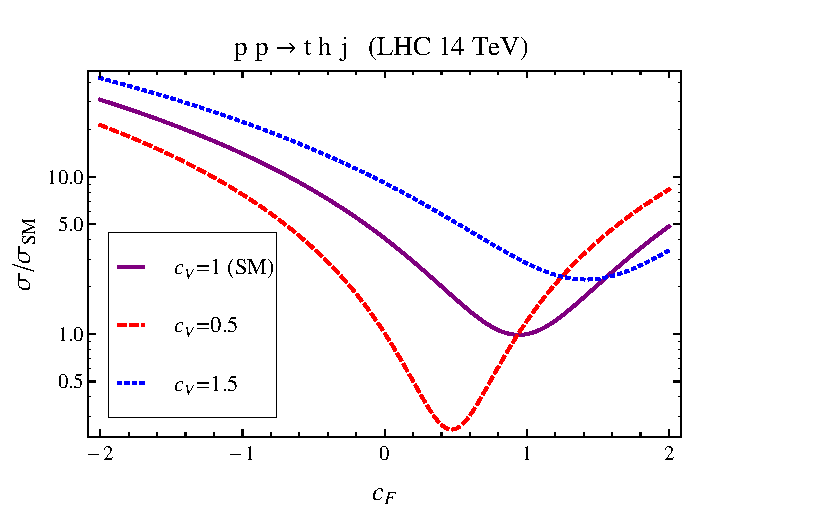
\includegraphics[scale=0.9]{thq_en}\\
\caption[Cross section for tHq process as a function of $\kappa_t$]{Cross section for \tHq process as a function of $\kappa_t$, normalized to the SM, for three values of $\kappa_V$. In the plot $c_f$ refers to the Higgs-fermion coupling which is dominated by the H-t coupling and represented here by $\kappa_t$. Solid, dashed and dotted lines correspond to $c_V \to \kappa_V= 1, 0.5, 1.5$ respectively. Note that for the SM ($\kappa_V=\kappa_t=1$), the destructive effect of the interference is maximal.} 
\label{thq_en}
\end{figure}

\begin{figure}[h!]
\centering
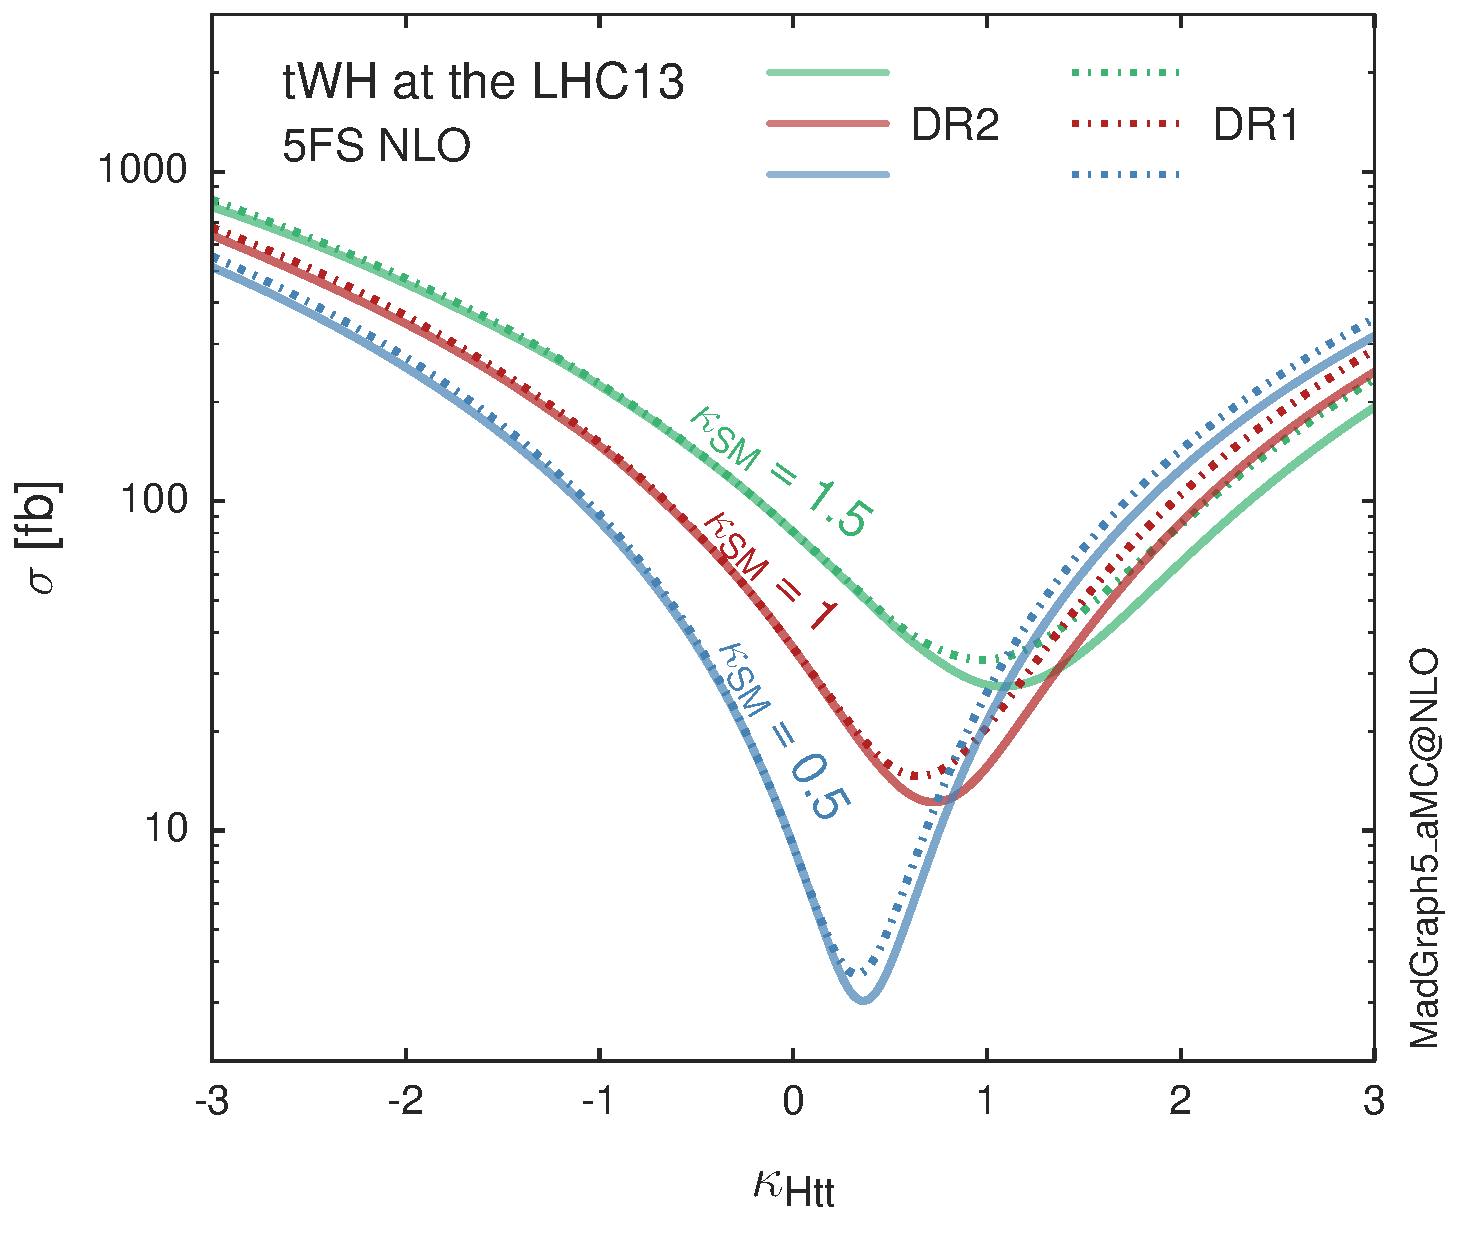
\includegraphics[scale=0.4]{thw_en}\\
\caption[Cross section for \tHW process as a function of $\kappa_{Htt}$]{Cross section for \tHW process as a function of $\kappa_{Htt}$, for three values of $\kappa_{SM}$ at $\sqrt{s}=13$ TeV. $\kappa_{Htt}^2=\sigma_{Htt}/\sigma_{Htt}^{SM}$ is a simple rescaling of the SM Higgs interactions.} 
\label{thw_en}
\end{figure}

A similar analysis is valid for the W-associated channel but, in that case, the interference is more complicated since there are more than two contributions and an additional interference with the production of Higgs boson and a top pair process(\ttH). The calculations are made using the so-called Diagram Removal (DR) technique where interfering diagrams are removed (or added) from the calculations in order to evaluate the impact of the removed contributions. DR1 was defined to neglect \ttH interference while DR2 was defined to take \ttH interference into account\cite{demartin}. As shown in Figure \ref{thw_en}, the \tHW cross section is enhanced from about 15 fb (SM: $\kappa_{Htt}=1$) to about 150 fb ($\kappa_{Htt}=-1$). Differences between curves for DR1 and DR2 help to gauge the impact of the interference with \ttH.\\      
Results of the calculations of the \tHq and \tHW cross sections at $\sqrt{s}=13$ TeV can be found in Reference \cite{yellow} and a summary of the results is presented in Table \ref{tab:th_xsec_en}.
\begin{center}
\begin{table}[h]
\centering
\begin{tabular}{lcll}\hline
                                                            & $\sqrt{s}$ TeV   & $\kappa_t=1$                        & $\kappa_t=-1$                   \\\hline
\multirow{2}{*}{$\sigma^{LO}$(\tHq)(fb)\cite{farina}}       & 8                & $\approx 17.4$                 & $\approx 252.7$            \\
                                                            & 14               & $\approx 80.4$                 & $\approx 1042$             \\\hline
\multirow{2}{*}{$\sigma^{NLO}$(\tHq)(fb)\cite{farina}}      & 8                & $18.28^{+0.42}_{-0.38}$        & $233.8^{+4.6}_{-0.0}$      \\
                                                            & 14               & $88.2^{+1.7}_{-0.0}$           & $982.8^{+28}_{-0.0}$       \\\hline
$\sigma^{LO}$(\tHq)(fb) \cite{biswas2}                      & 14               & $\approx 71.8$                 & $\approx 893$              \\
$\sigma^{LO}$(\tHW)(fb) \cite{biswas2}                      & 14               & $\approx 16.0$                 & $\approx 139$              \\\hline
\multirow{3}{*}{$\sigma^{NLO}$(\tHq)(fb)\cite{yellow}}      & 8                & $18.69^{+8.62\%}_{-17.13\%}$   & -                          \\
                                                            & 13               & $74.25^{+7.48\%}_{-15.35\%}$   & $848^{+7.37\%}_{-13.70\%}$ \\
                                                            & 14               & $90.10^{+7.34\%}_{-15.13\%}$   & $1011^{+7.24\%}_{-13.39\%}$\\\hline
$\sigma^{LO}$(\tHW)(fb)\cite{demartin}                      & 13               & $15.77^{+15.91\%}_{-15.76\%}$  & -                          \\
$\sigma^{NLO} DR1$(\tHW)(fb)\cite{demartin}                 & 13               & $21.72^{+6.52\%}_{-5.24\%}$    & $\approx 150$              \\
$\sigma^{NLO} DR2$(\tHW)(fb)\cite{demartin}                 & 13               & $16.28^{+7.34\%}_{-15.13\%}$   & $\approx 150$              \\\hline
\end{tabular}
\caption[Predicted enhancement of the \tHq and \tHW cross sections at LHC]{Predicted enhancement of the \tHq and \tHW cross sections at LHC for $\kappa_V=1$ and $\kappa_t= \pm1$ at LO and NLO; the cross section enhancement of more that a factor of 10 is due to the flippling in the sign of the H-t coupling with respect to the SM one.}
\label{tab:th_xsec_en}
\end{table}
\end{center}

%% \begin{center}
%% \begin{table}[h]
%% \centering
%% \begin{tabular}{lcll}\hline
%%                                                             & $\sqrt{s}$ TeV   & $\kappa_t=1$                        & $\kappa_t=-1$                   \\\hline
%% \multirow{2}{*}{$\sigma^{LO}$(\tHq)(fb)\cite{farina}}       & 8                & $\approx 17.4$                 & $\approx 252.7$            \\
%%                                                             & 14               & $\approx 80.4$                 & $\approx 1042$             \\\hdashline
%% $\sigma^{LO}$(\tHq)(fb) \cite{biswas2}                      & 14               & $\approx 71.8$                 & $\approx 893$              \\
%% $\sigma^{LO}$(\tHW)(fb) \cite{biswas2}                      & 14               & $\approx 16.0$                 & $\approx 139$              \\%\hline
%% $\sigma^{LO}$(\tHW)(fb)\cite{demartin}                      & 13               & $15.77^{+15.91\%}_{-15.76\%}$  & -                          \\\hline
%% \multirow{2}{*}{$\sigma^{NLO}$(\tHq)(fb)\cite{farina}}      & 8                & $18.28^{+0.42}_{-0.38}$        & $233.8^{+4.6}_{-0.0}$      \\
%%                                                             & 14               & $88.2^{+1.7}_{-0.0}$           & $982.8^{+28}_{-0.0}$       \\\hdashline
%% \multirow{3}{*}{$\sigma^{NLO}$(\tHq)(fb)\cite{yellow}}      & 8                & $18.69^{+8.62\%}_{-17.13\%}$   & -                          \\
%%                                                             & 13               & $74.25^{+7.48\%}_{-15.35\%}$   & $848^{+7.37\%}_{-13.70\%}$ \\
%%                                                             & 14               & $90.10^{+7.34\%}_{-15.13\%}$   & $1011^{+7.24\%}_{-13.39\%}$\\\hdashline
%% $\sigma^{NLO} DR1$(\tHW)(fb)\cite{demartin}                 & 13               & $21.72^{+6.52\%}_{-5.24\%}$    & $\approx 150$              \\
%% $\sigma^{NLO} DR2$(\tHW)(fb)\cite{demartin}                 & 13               & $16.28^{+7.34\%}_{-15.13\%}$   & $\approx 150$              \\\hline
%% \end{tabular}
%% \caption[Predicted enhancement of the \tHq and \tHW cross sections at LHC]{Predicted enhancement of the \tHq and \tHW cross sections at LHC for $\kappa_V=1$ and $\kappa_t= \pm1$ at LO and NLO; the cross section enhancement of more that a factor of 10 is due to the flippling in the sign of the H-t coupling with respect to the SM one.}
%% \label{tab:th_xsec_en}
%% \end{table}
%% \end{center}

%______________________ cp phase ______________________
\section{The CP-mixing in tH processes}\label{sec:cp}

In addition to the sensitivity to sign of the H-t coupling, \tHq and \tHW processes have been proposed as a tool to investigate the possibility of a H-t coupling that does not conserve CP\cite{maltoni2,demartin,ellis}. Current experimental results are consistent with SM H-V and H-t couplings; however, negative H-t coupling is not excluded completely \cite{comb_ht_couplings}.\\

In this thesis, the sensitivity of \tH processes to CP-mixing is also studied in the effective field theory framework and based in References \cite{maltoni2,demartin}; a generic particle ($X_0$) of spin-0 and a general CP violating interaction with the top quark, can couple to scalar and pseudoscalar fermionic densities. The H-W interaction is assumed to be SM-like. The Lagrangian modeling the H-t interaction is given by

\beqn
\Lagr_0^t = -\bar\psi_t\left(c_{\alpha}\kappa_{Htt}g_{Htt}+i s_{\alpha}\kappa_{Att}g_{Att}\gamma_5 \right)\psi_t X_0,
\label{eq:l_cp}
\eeqn

\noindent where $\alpha$ is the CP-mixing phase, $c_\alpha\equiv\cos\alpha$ and $s_\alpha\equiv\sin\alpha$, $\kappa_{Htt}$ and $\kappa_{Att}$ are real dimensionless rescaling parameters\footnote{analog to $\kappa_t$ and $\kappa_V$}, $g_{Htt}=g_{Att}=m_t/v=y_t/\sqrt{2}$ and $v\sim 246$ GeV is the Higgs vacuum expectation value. In this parametrization, it is easy to recover three special cases

\begin{itemize}
\item CP-even coupling $\to \alpha=0^o$  
\item CP-odd coupling $\to \alpha=90^o$
\item SM coupling $\to \alpha=0^o$ and $\kappa_{Htt}=1$  
\end{itemize}

The loop induced $X_0$ coupling to gluons can also be described in terms of the parametrization above, according to

\beqn
\Lagr_0^{g} = -\frac{1}{4}\left(c_{\alpha}\kappa_{Hgg}g_{Hgg}G_{\mu\nu}^aG^{a,\mu\nu}+s_{\alpha}\kappa_{Agg}g_{Agg}G_{\mu\nu}^a\widetilde G^{a,\mu\nu} \right)X_0.
\label{eq:l_Hglu}
\eeqn

\noindent where $g_{Hgg}=-\alpha_s/3\pi v$ and $g_{Agg}= \alpha_s/2\pi v$.  Under the assumption that the top quark dominates the gluon-fusion process at LHC energies, $\kappa_{Hgg} \to \kappa_{Htt}$ and  $\kappa_{Agg} \to \kappa_{Att}$, so that the ratio between the gloun-gluon fusion cross section for $X_0$ and for the SM Higgs prediction can be written as     

\beqn
\frac{\sigma_{NLO}^{gg \to X_0} }{\sigma_{NLO,SM}^{gg \to H}}=  c^2_\alpha\kappa^2_{Htt}+s^2_\alpha \left( \kappa_{Att}\frac{g_{ Agg}}{g_{Hgg}} \right)^2.
\label{eq:GFrate}
\eeqn

If the rescaling parameters are set to

\beqn
\kappa_{Htt}=1, \qquad \kappa_{Att}= \left|\frac{g_{Hgg}}{g_{Agg}}\right|=\frac{2}{3}.
\eeqn

\noindent the gluon-fusion SM cross section is reproduced for every value of the CP-mixing angle $\alpha$; therefore, by imposing that condition to the Lagrangian density \ref{eq:l_cp}, the CP-mixing angle is not constrained by current data. Figure \ref{xsec_alpha_thq} shows the NLO cross sections for t-channel $tX_0$(blue) and $t\bar{t}X_0$ (red) associated production processses as a function of the CP-mixing angle $\alpha$. $X_0$ is a generic spin-0 particle with top quark CP-violating coupling. Rescaling factors $\kappa_{Htt}$ and  $\kappa_{Att}$ have been set to reproduce the SM gluon-fusion cross sections.   

\begin{figure}[h!]
\centering
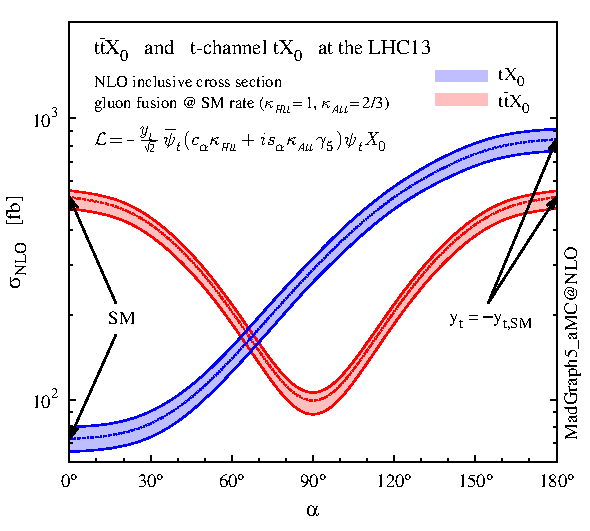
\includegraphics[scale=1.2]{xsec_alpha_thq}
\caption[NLO cross section for $tX_0$ and $t\bar{t}X_0$.]{NLO cross sections for t-channel $tX_0$(blue) and $t\bar{t}X_0$ (red) associated production processses as a function of the CP-mixing angle $\alpha$. $X_0$ is a generic spin-0 particle with top quark CP-violating coupling \cite{maltoni2}.} 
\label{xsec_alpha_thq}
\end{figure}

It is interesting to notice that the $tX_0$ croos section is enhanced, by a factor of about 10, when a continuous rotation in the scalar-pseudoscalar plane is applied; this enhancement is similar to the enhancement produced when the H-t coupling is flipped in sign with respect to the SM ($y_t=-y_{t,SM}$ in the plot), as showed in Section \ref{sec:thq}. In contrast, the degeneracy in the $t\bar{t}X_0$ cross section is still present given that it depends quadratically on the H-t coupling, but more instersting is to notice that $t\bar{t}X_0$ cross section is exceeded by $tX_0$ cross section after $\alpha\sim 60^o$.
\begin{figure}[h!]
\centering
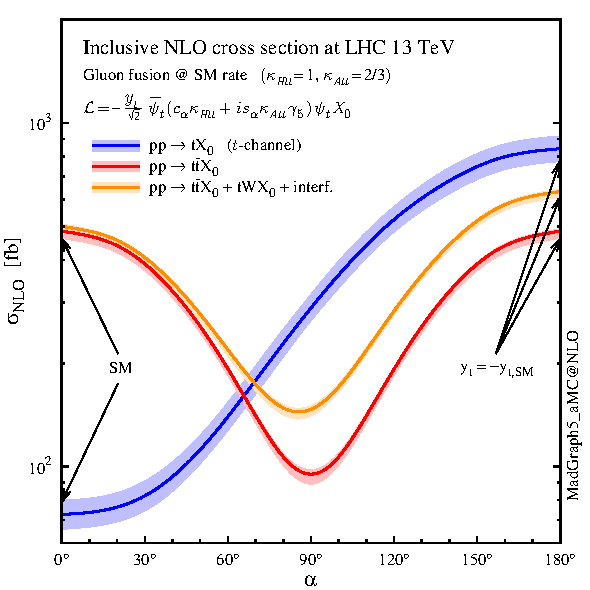
\includegraphics[scale=1.1]{xsec_alpha_thw}
\caption[NLO cross section for $tWX_0$, $t\bar{t}X_0$.]{NLO cross sections for t-channel $tX_0$(blue), $t\bar{t}X_0$ (red) associated production processses and combined $tWX_0 + t\bar{t}X_0$ (including interference) production as a function of the CP-mixing angle $\alpha$\cite{maltoni2}.} 
\label{xsec_alpha_thw}
\end{figure}

A similar parametrization can be used to investigate the \tHW process sensitivity to CP-violating H-t coupling. As said in \ref{sec:thq}, the interference in the W-associated channel is more complicated because there are more than two contributions and also there is interference with the \ttH production process.\\

Figure \ref{xsec_alpha_thw} shows the NLO cross sections for t-channel $tX_0$(blue), $t\bar{t}X_0$ (red) associated production and for the combined  $tWX_0 + t\bar{t}X_0 +$ interference (orange) as a function of the CP-mixing angle. It is clear that the effect of the interference in the combined case is the lifting of the degeneracy present in the $t\bar{t}X_0$ production. The constructive interference enhances the cross section from about 500 fb at SM ($\alpha=0$) to about 600 fb ($\alpha=180^o \to y_t=-y_{t,SM}$).  

An analysis combining \tHq and \tHW processes will be made in this thesis taking advantage of the sensitivity improvement.

\section{Experimantal status of the anomalous Higg-fermion coupling.}

\begin{figure}[h!]
\centering
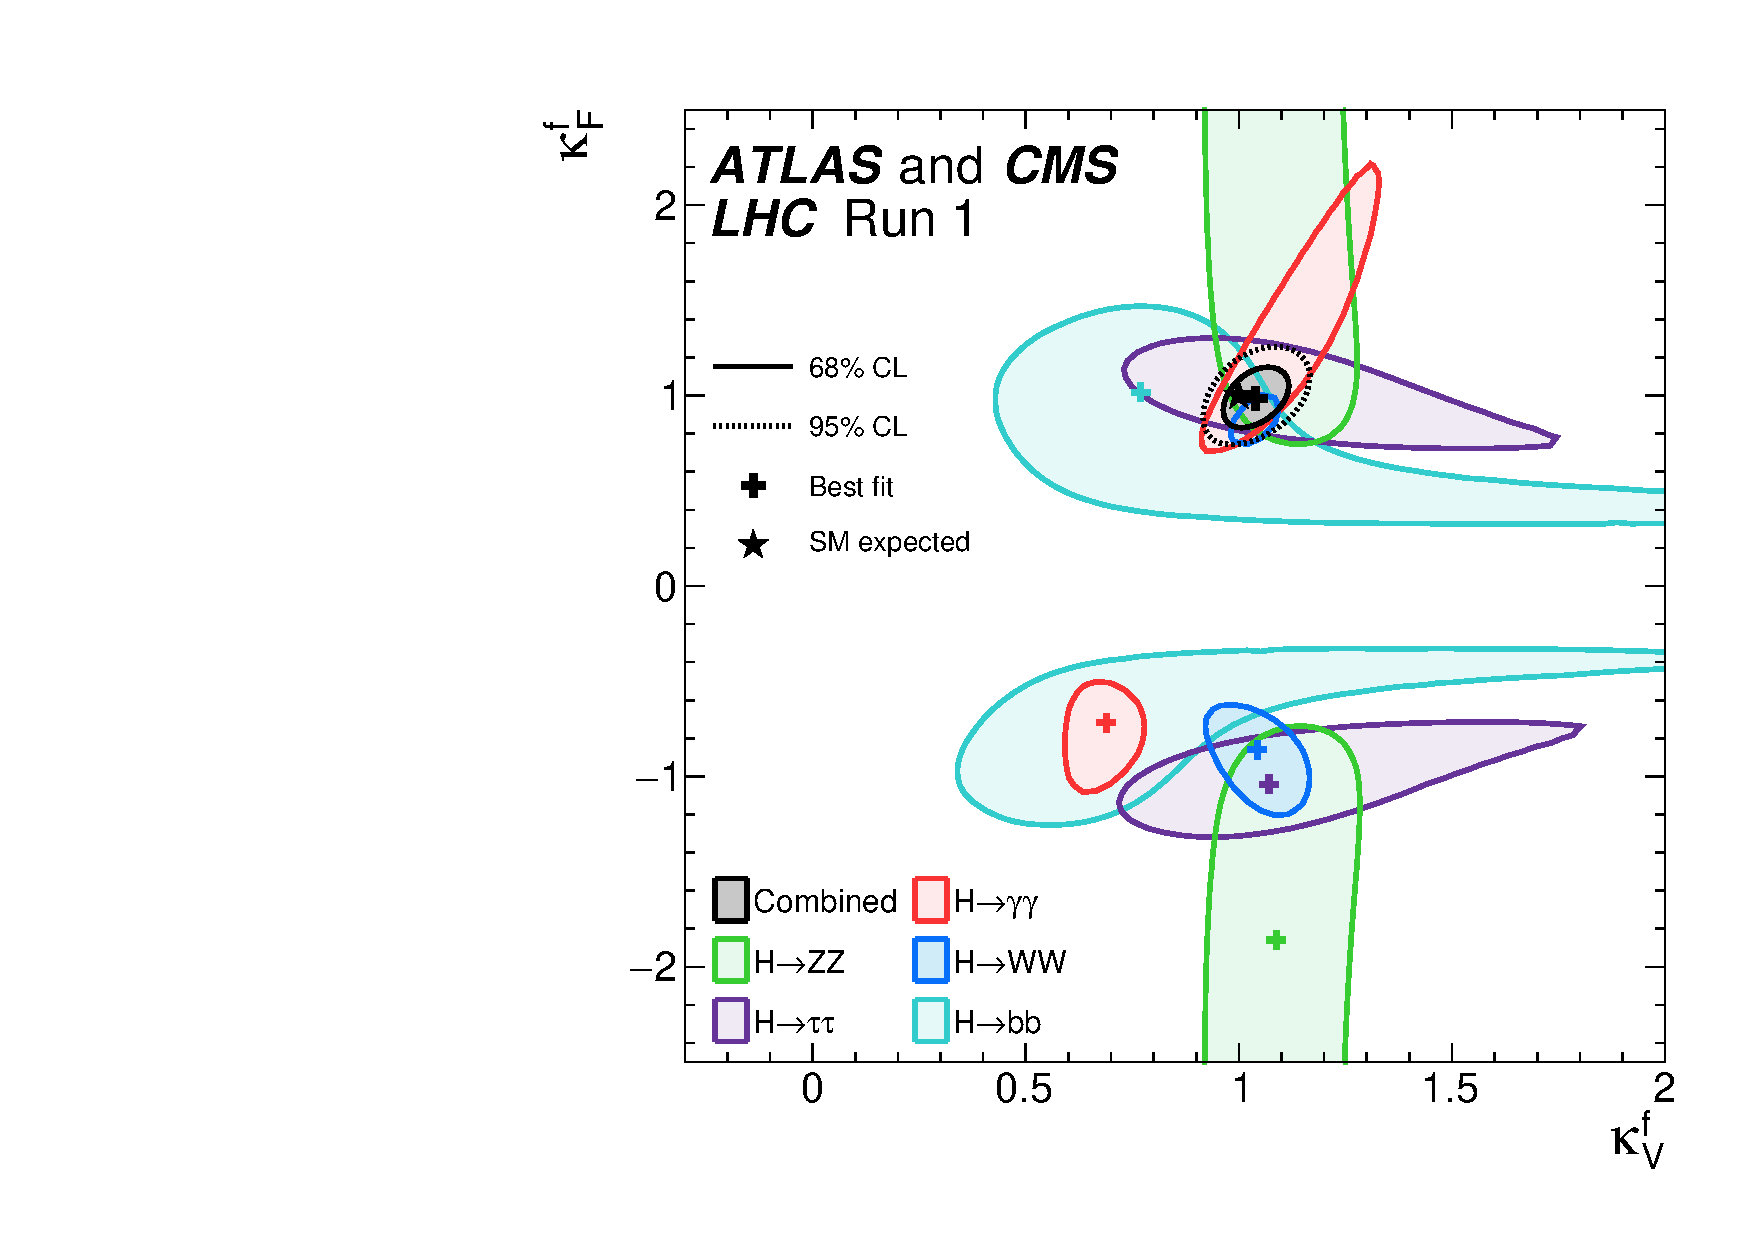
\includegraphics[scale=0.5]{kt_kv}
\caption[Two dimentional $\kappa_t$-$\kappa_V$ plot of the coupling modifiers. ATLAS and CMS combination.]{Combination of the  ATLAS and CMS fits for coupling modifiers $\kappa_t$-$\kappa_V$; also shown the individual decay channels combination and their global combination. No assumptions have been made on the sign of the coupling modifiers\cite{comb_ht_couplings}.} 
\label{fig:kt_kv}
\end{figure}
 
ATLAS and CMS have performed analysis of the anomalous H-f coupling by making likelihood scans for the two coupling modifiers, $\kappa_t$ and $\kappa_V$, under the assumption that $\kappa_Z=\kappa_W=\kappa_V$ and $\kappa_t=\kappa_\tau=\kappa_b=\kappa_f$. Figure \ref{fig:kt_kv} shows the result of the combination of ATLAS and CMS fits; also the individual decay channels combination and the global combination results are shown.

\noindent While all the channels are compatible for positive values of the modifiers, for negative values of $\kappa_t$ there is no compatibility. The best fit for individual channels is compatible with negative values of $\kappa_t$ except for the $H\to bb$ channel which is expected to be the most sensitive channel; therefore, the best fit for the global fit yields $\kappa_t\geq0$. Thus, the anomaluos H-t coupling cannot be excluded completely. 

\chapter{The CMS experiment at the LHC}\label{ch:cms}

\section{Introduction}\label{sec:cms_intro}
\noindent Located in the Swiss-French border, the European Council for Nuclear Research (CERN) is the largest scientific organization leading the particle physics research. About 13000 people in a broad range of fields including users, students, scientists, engineers among others, contribute to the data taking and analysis, with the goal of unveiling the secrets of the nature and revealing the fundamental structure of the universe. CERN is also the home of the Large Hadron Collider (LHC), the largest circular particle accelerator around the world, where protons (or heavy ions) traveling close to the speed of light, are made to collide. These collisions open a window to investigate how particles (and their constituents if they are composite) interact with each other, providing clues about the laws of the nature. This chapter present an overview of the LHC structure and operation. A detaled description of the CMS detector is offered, given that the data used in this thesis have been taken with this detector.     

\section{The LHC}

\noindent With 27 km of circunference, the LHC is currently the largest and most powerful accelerator in the world. It is installed in the same tunnel where the large Electron-Positron (LEP) collider was located, taking advantage of the existing infraestructure. The LHC is also the larger accelerator in the CERN's accelerator complex and is assisted by several successive accelerating stages before the particles are injected into the LHC ring where they reach their maximum eneregy (see figure \ref{fig:cern}).

\begin{figure}[!h]
  \centering
  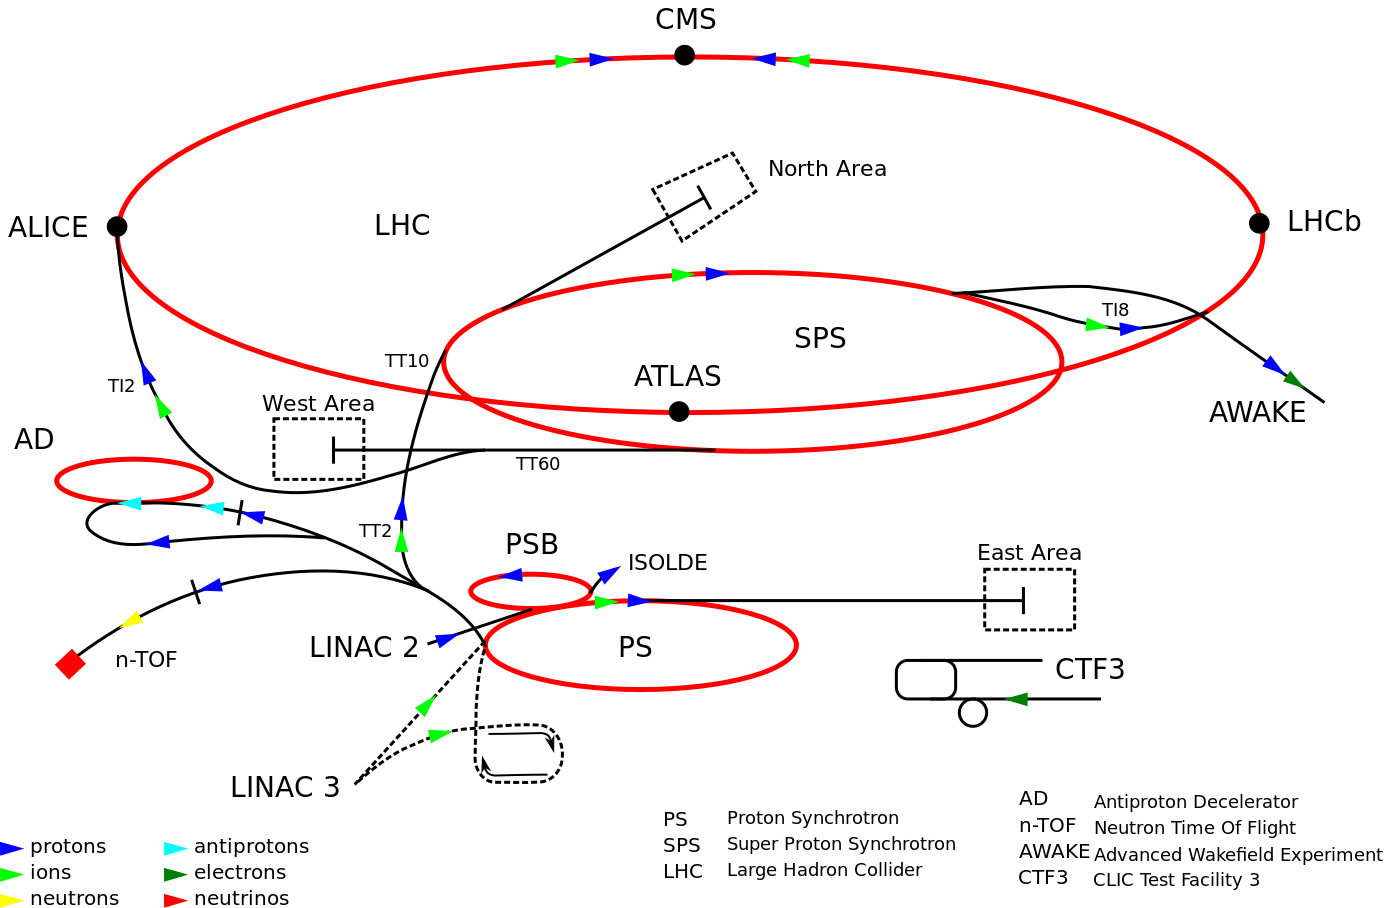
\includegraphics[width=0.7\textwidth]{cern_ac}
  \caption[CERN accelerator complex]{CERN accelerator complex. Blue arrows show the path followed by protons along the acceleration process \cite{cern}.}\label{fig:cern}
\end{figure}

\noindent LHC run in three modes depending on the particles being accelerated

\begin{itemize}
\item Proton-Proton collisions (pp) for multiple physics experiments.
\item Lead-Lead collisions (Pb-Pb) for heavy ion experiments. 
\item Proton-Lead collisions (p-Pb) for quark-gluon plasma experiments.
\end{itemize}

\begin{figure}[!h]
\centering
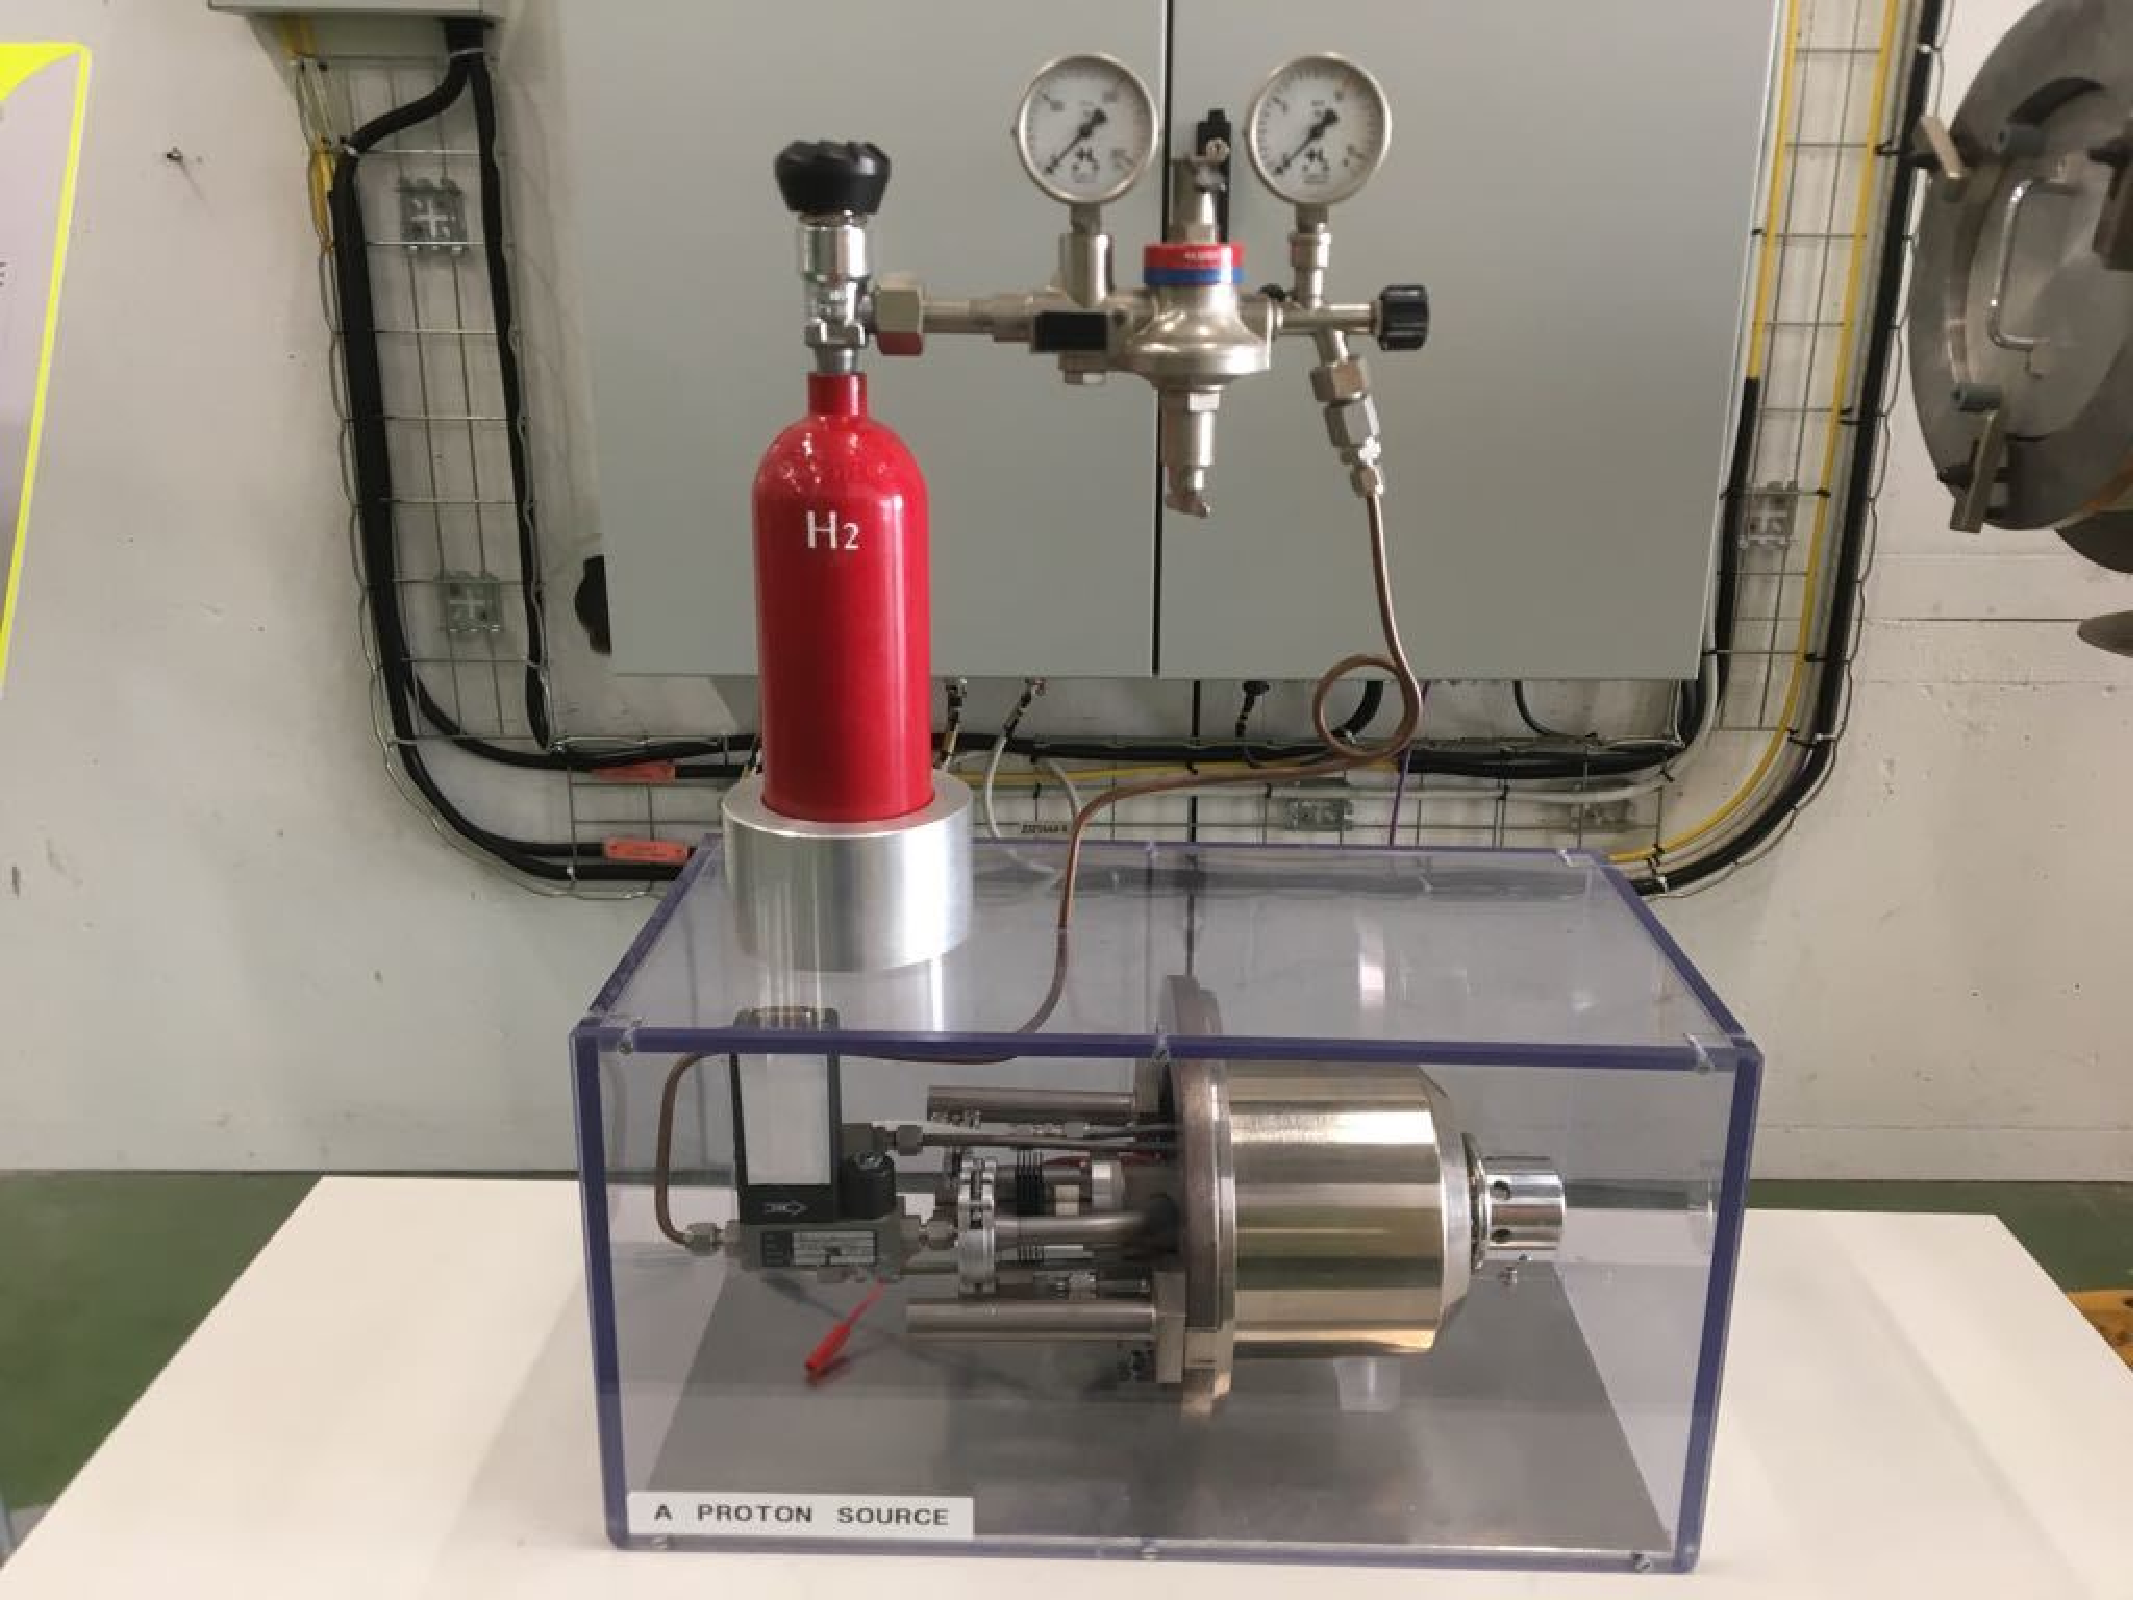
\includegraphics[width=4.5cm,height=3.3cm]{hbottle}
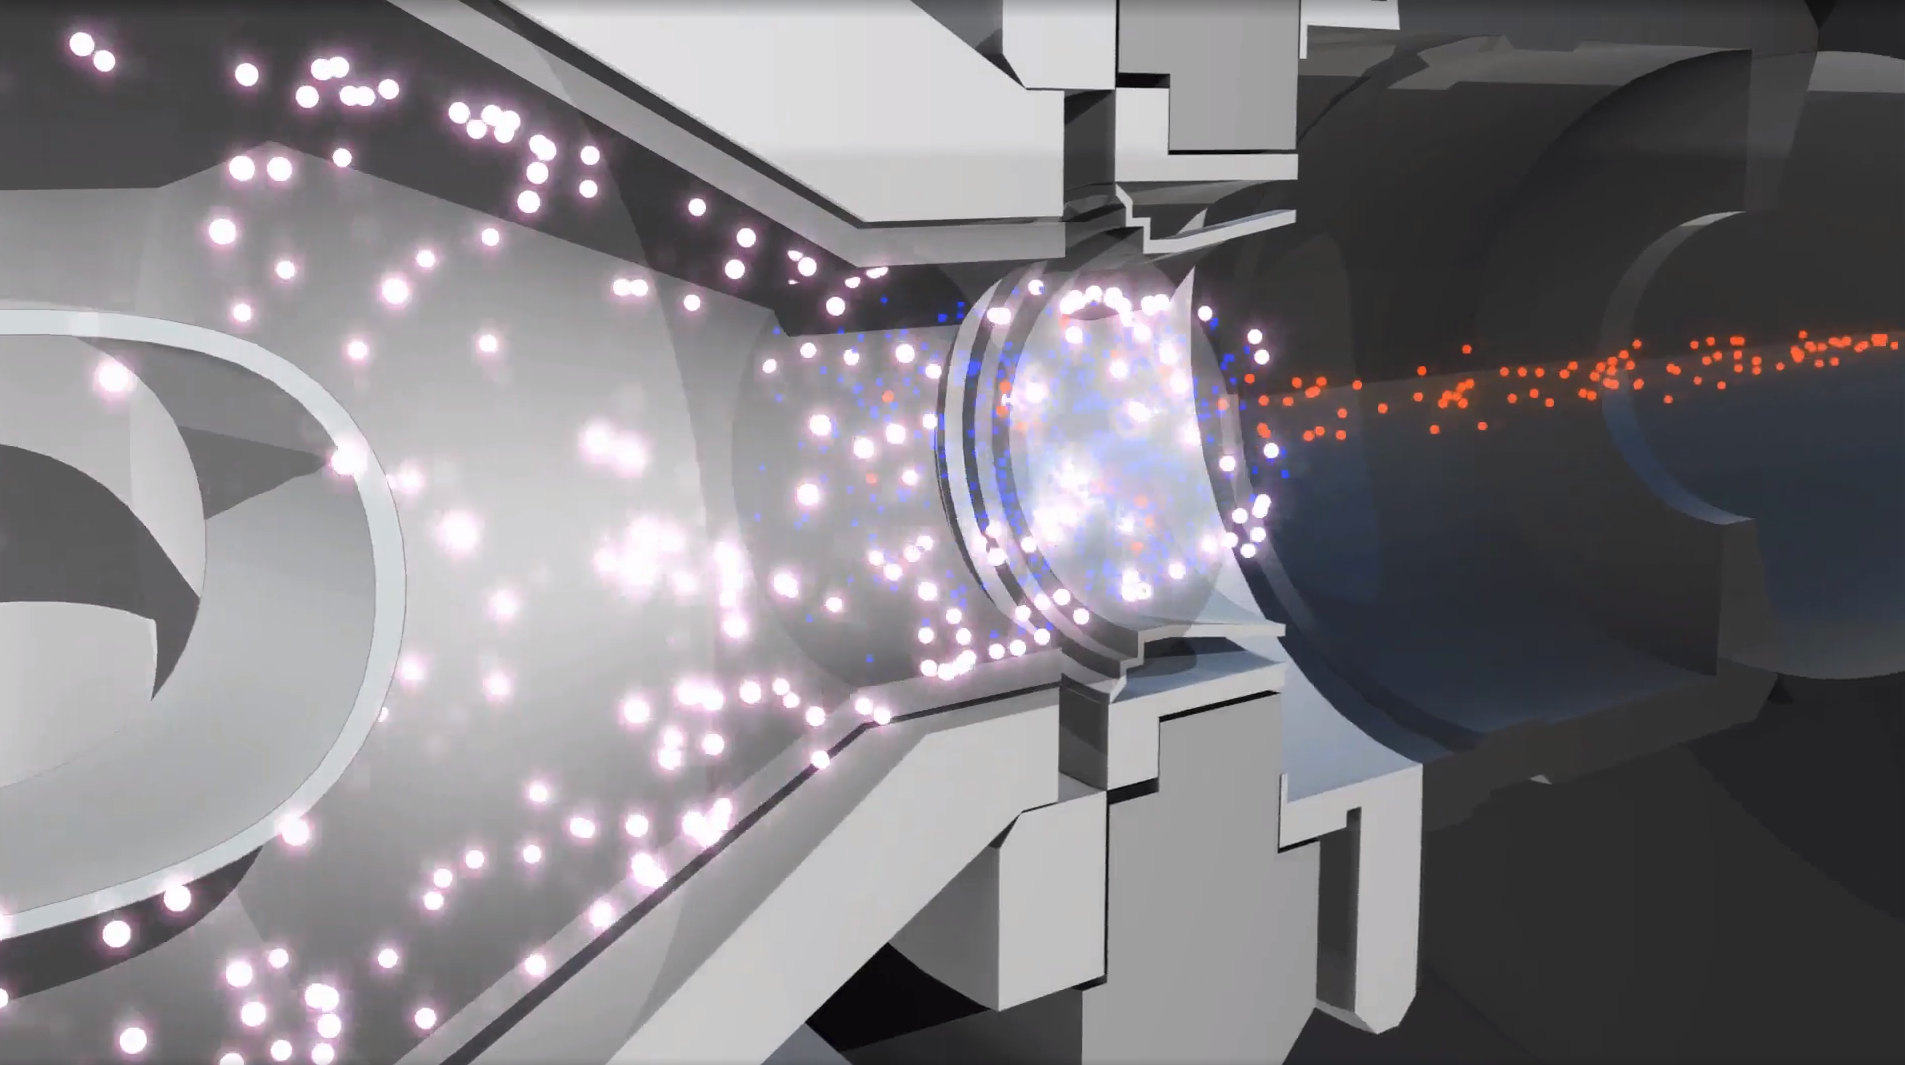
\includegraphics[width=6.0cm,height=3.3cm]{proton_source}\\
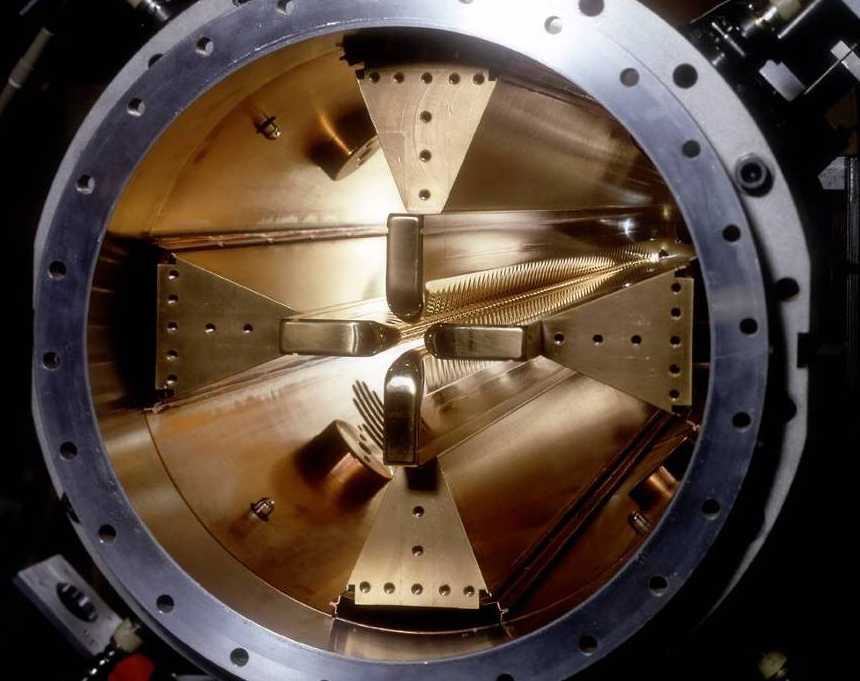
\includegraphics[width=4.5cm,height=3.3cm]{rfq2}
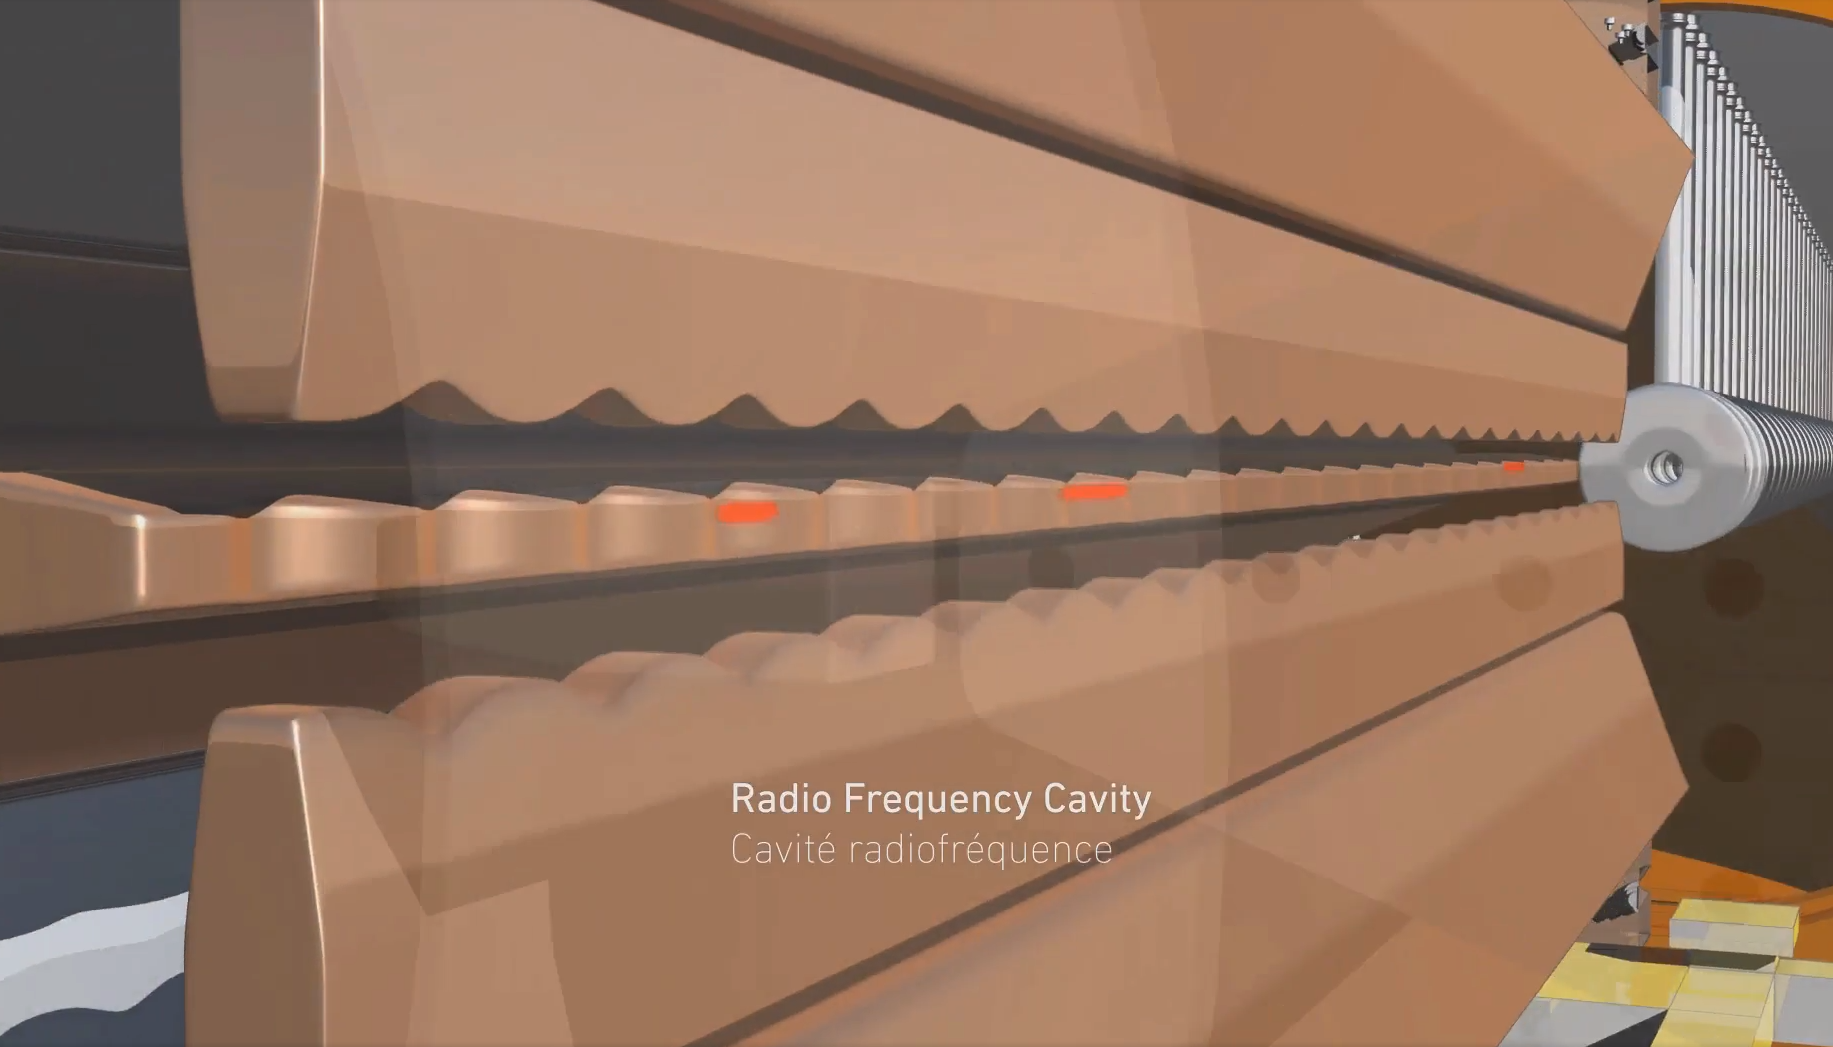
\includegraphics[width=6.0cm,height=3.3cm]{rfq3}
\caption[LHC protons source and first acceleration stage.]{LHC protons source and first acceleration stage. Top: the bottle contains hydrogen gas (white dots) which is injected into the metal cylinder to be broken down into electrons(blue dots) and protons(red dots); Bottom: the obtained protons are directed towards the radio frequency quadrupole which perform the first acceleration, focus the beam and create the bunches of protons.\cite{rfq2,video}}\label{fig:hbottle}
\end{figure}

\noindent In this thesis pp collisions will be considered.\\

\noindent Collection of protons starts with hydrogen atoms taken from a bottle, containing hydrogen gas, and injecting them in a metal cillinder; hydrogen atoms are broken down into electrons and protons by an intense electric field (see figure\ref{fig:hbottle} top). The resulting protons leave the metal cylinder towards a radio frecuency quadrupole (RFQ) that focus the beam, accelerate the protons and create the packets of protons called bunches. In the RFQ, an electric field is generated by a RF wave at a frecuency that matches the resonance frecuency of the cavity where the electrodes are contained. The beam of protons traveling on the RFQ axis experience an alternating electric field gradient that generates the focusing forces.\\

\noindent In order to accelerate the protons, a longitudinal time-variying electric field component is added to the system; it is done by giving the electrodes a sinus-like profile as shown in figure \ref{fig:hbottle} bottom. By matching the speed and phase of the protons with the longitudinal electric field the bunching is performed; protons synchronized with the RFQ (synchronous proton) does not feel an accelerating force, but those protons in the beam that have more (or less) energy than the synchronous proton (asynchronous protons) will feel a decelerating (accelerating) force; therefore, asynchronous protons will oscillate around the synchronous ones forming bunches of protons \cite{rfq}. From the RFQ emerges protons with energy 750 keV in bunches of about $1.15 \times 10^{11}$ protons\cite{lyndon}.        

\begin{figure}[!h]
  \centering
  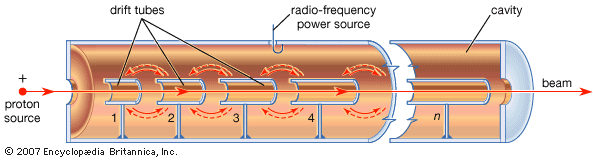
\includegraphics[scale=0.5]{linac}
  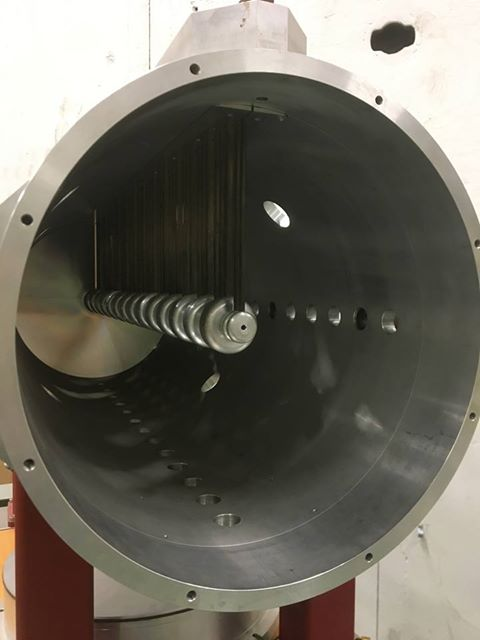
\includegraphics[width=3.0cm,height=3.0cm]{linac2}
  \caption [The LINAC2 accelerating system at CERN.]{The LINAC2 accelerating system at CERN. Radio frecuency (RF) generated electric fields create acceleration and deceleration zones inside the cavity; deceleration zones are blocked by drift tubes where quadrupole magnets focus the proton beam.\cite{linac}}\label{fig:linac}
\end{figure}

\noindent Proton bunches coming from the RFQ goes to the linear accelerator 2 (LINAC2) where they are accelerated to reach 50 MeV energy. In the LINAC2 stage, acceleration is performed using radio frecuency generated electric fields which create zones of acceleration and deceleration as shown in figure \ref{fig:linac}. In the decelerations zones the electric field is blocked using drift tubes where protons are free to drift while quadrupole magnets focus the beam.\\   

\noindent The beam coming from LINAC2 is injected into the proton synchrotron booster (PSB) to reach 1.4 GeV in energy. The next acceleration is provided at the proton synchrotron (PS) up to 26 GeV, followed by the injection into the super proton synchrotron (SPS) where protons are accelerated to 450 GeV. Finally, protons are injected into the LHC where they are accelerated to the target energy of 6.5 TeV.
\noindent PSB, PS, SPS and LHC accelerate protons using the same RF acceleration technic described before. 

\begin{figure}[!h]
\centering
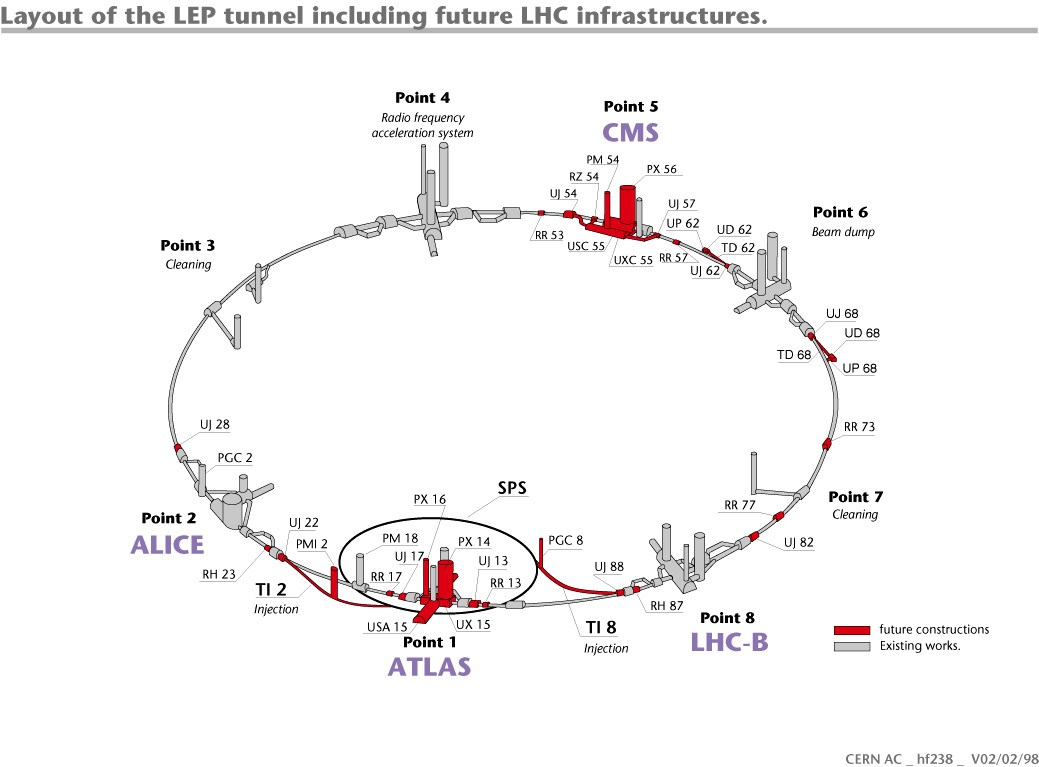
\includegraphics[scale=0.6]{lep}
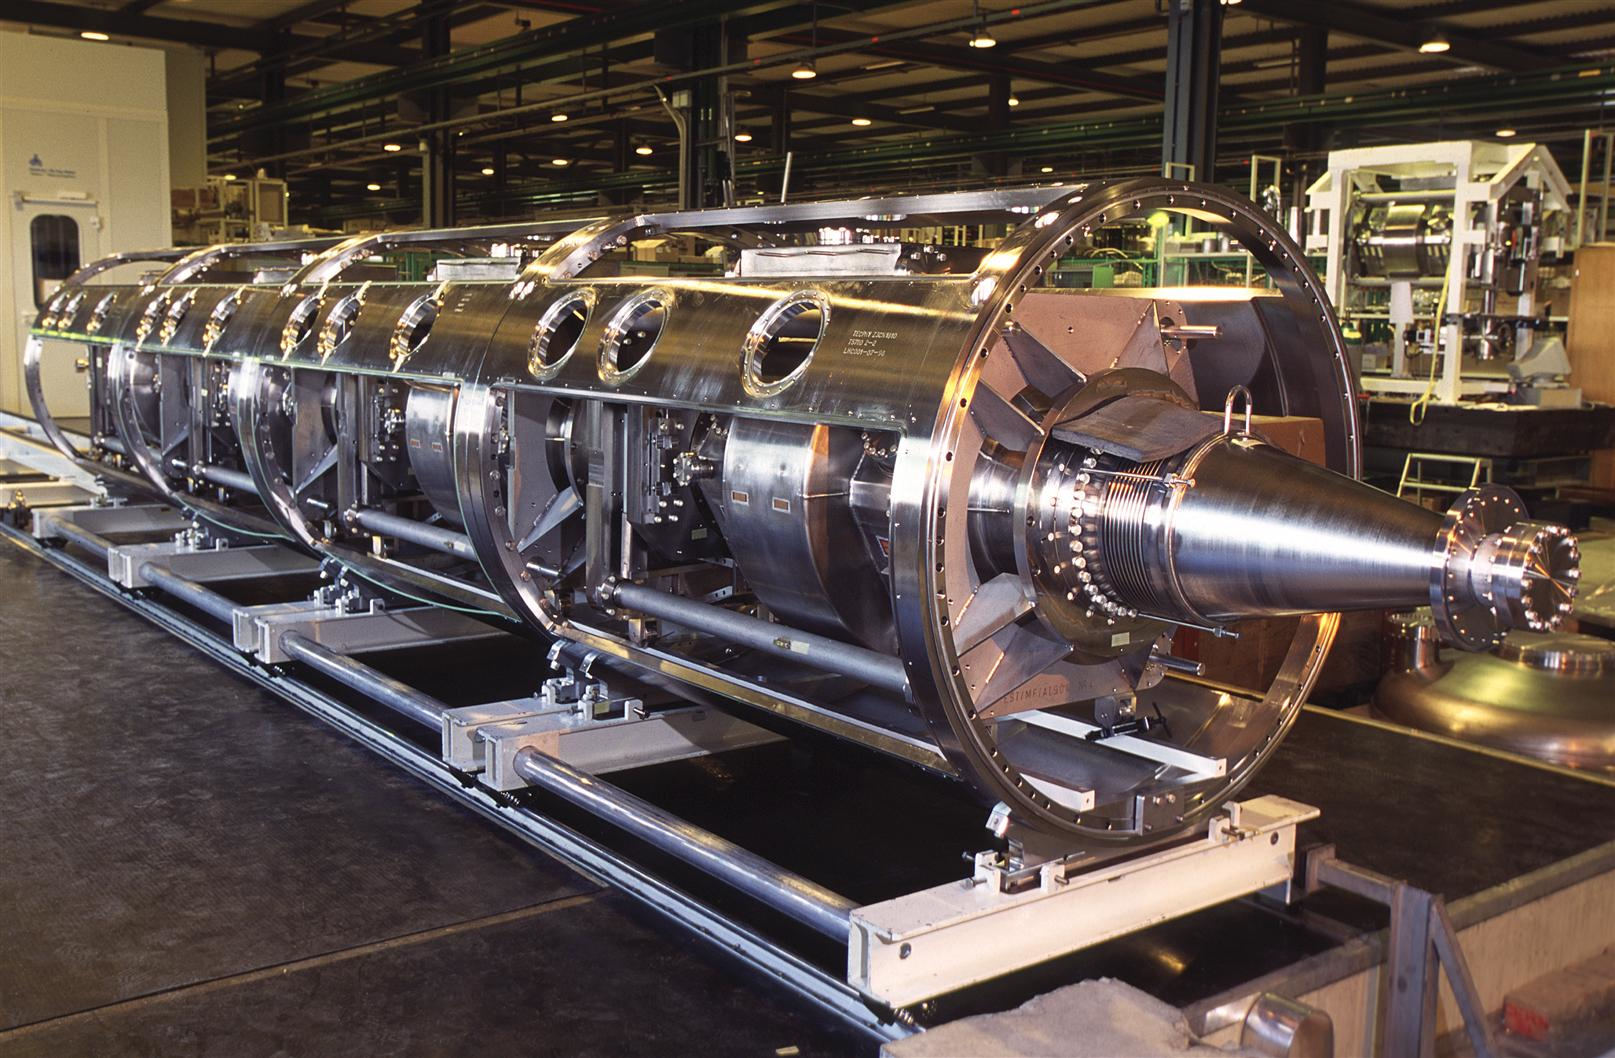
\includegraphics[width=7cm,height=4.2cm]{lhc_rfc}
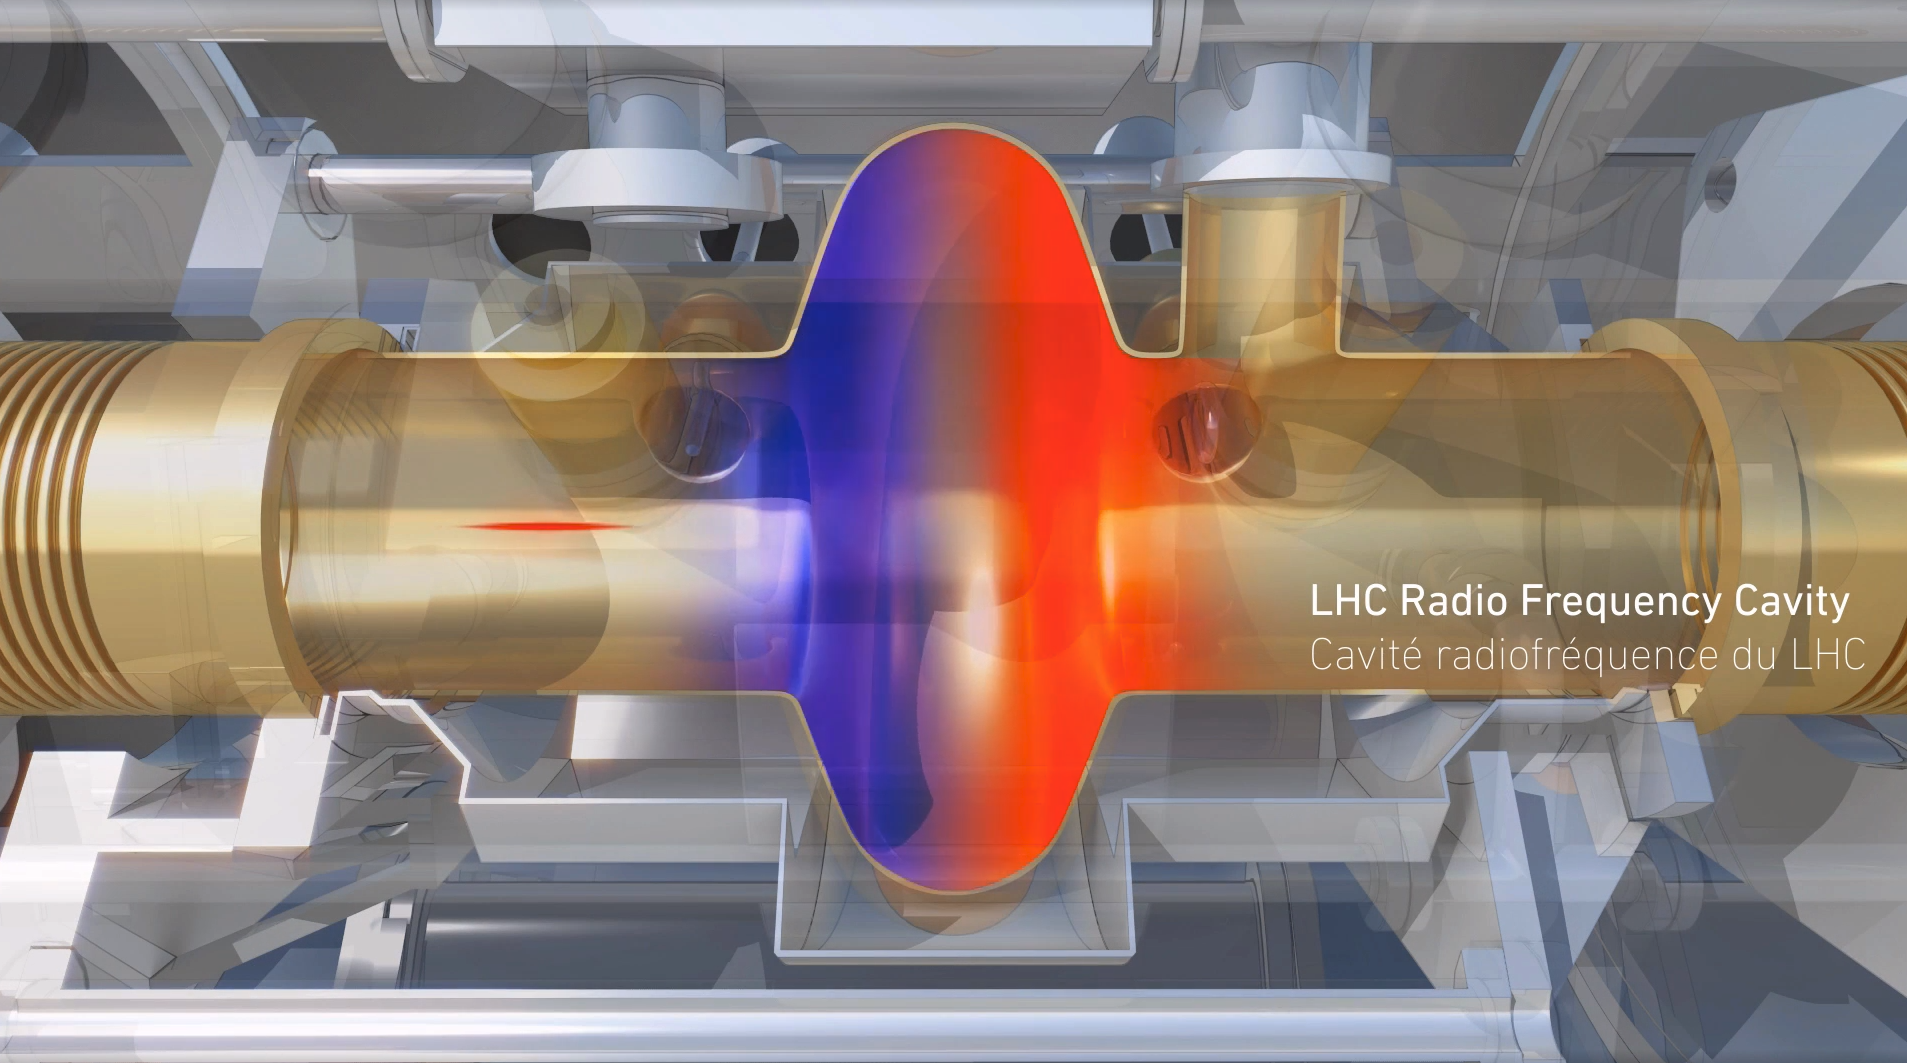
\includegraphics[scale=0.15]{rfc_lhc}
\caption[LHC layout and RF cavities module.]{Top: LHC layout. The red zones indicate the infrastructure additions to the LEP installations, built to accomodate the ATLAS and CMS experiments which exceed the size of the former experiments located there\cite{lep}. Bottom: LHC RF cavities. A module accomodates 4 cavities that accelerate protons and preserve the bunch structure of the beam.\cite{video,lhc_rfc}}\label{fig:lep_rfc}
\end{figure}

\noindent LHC have a system of 16 RF cavities located in the so-called point 4, as shown in figure \ref{fig:lep_rfc} top, tunned at a frecuency of 400 MHz and the protons are carefully timed so additionally to the acceleration effect the bunch structure of the beam is preserved. Bottom side of figure \ref{fig:lep_rfc} shows a picture of a Rf module composed of 4 RF cavities working in a superconducting state at 4.5 K; also is showed a representation of the accelerating electric field that accelerates the protons in the bunch.\\ 

\noindent While protons are accelerated in one section of the LHC ring, where the RF cavities are located, in the rest of their path they have to be kept in the curved trajectory defined by the LHC ring. Technically, LHC is not a perfect circle; RF, injection, beam dumping, beam cleaning and sections before and after the experimental points where protons collide are all straight sections. In total, there are 8 arcs 2.45 Km long each and 8 straight sections 545 m long each. In order to curve the proton's trajectory in the the arc sections, superconducting dipole magnets are used.\\               

\noindent Inside the LHC ring, there are two proton beams traveling in opposite directions in two separated beam pipes; the beam pipes are kept at ultra high vacuum ($\sim 10^{-9}$ Pa) to ensure that there are no particles that interact with the proton beams. The superconducting dipole magnets used in LHC are made of a NbTi alloy, capable of transporting currents of about $12000$ A when cooled at a temperature below 2K using liquid helium (see figure \ref{fig:lhcdipole}).

\begin{figure}[!h]
\centering
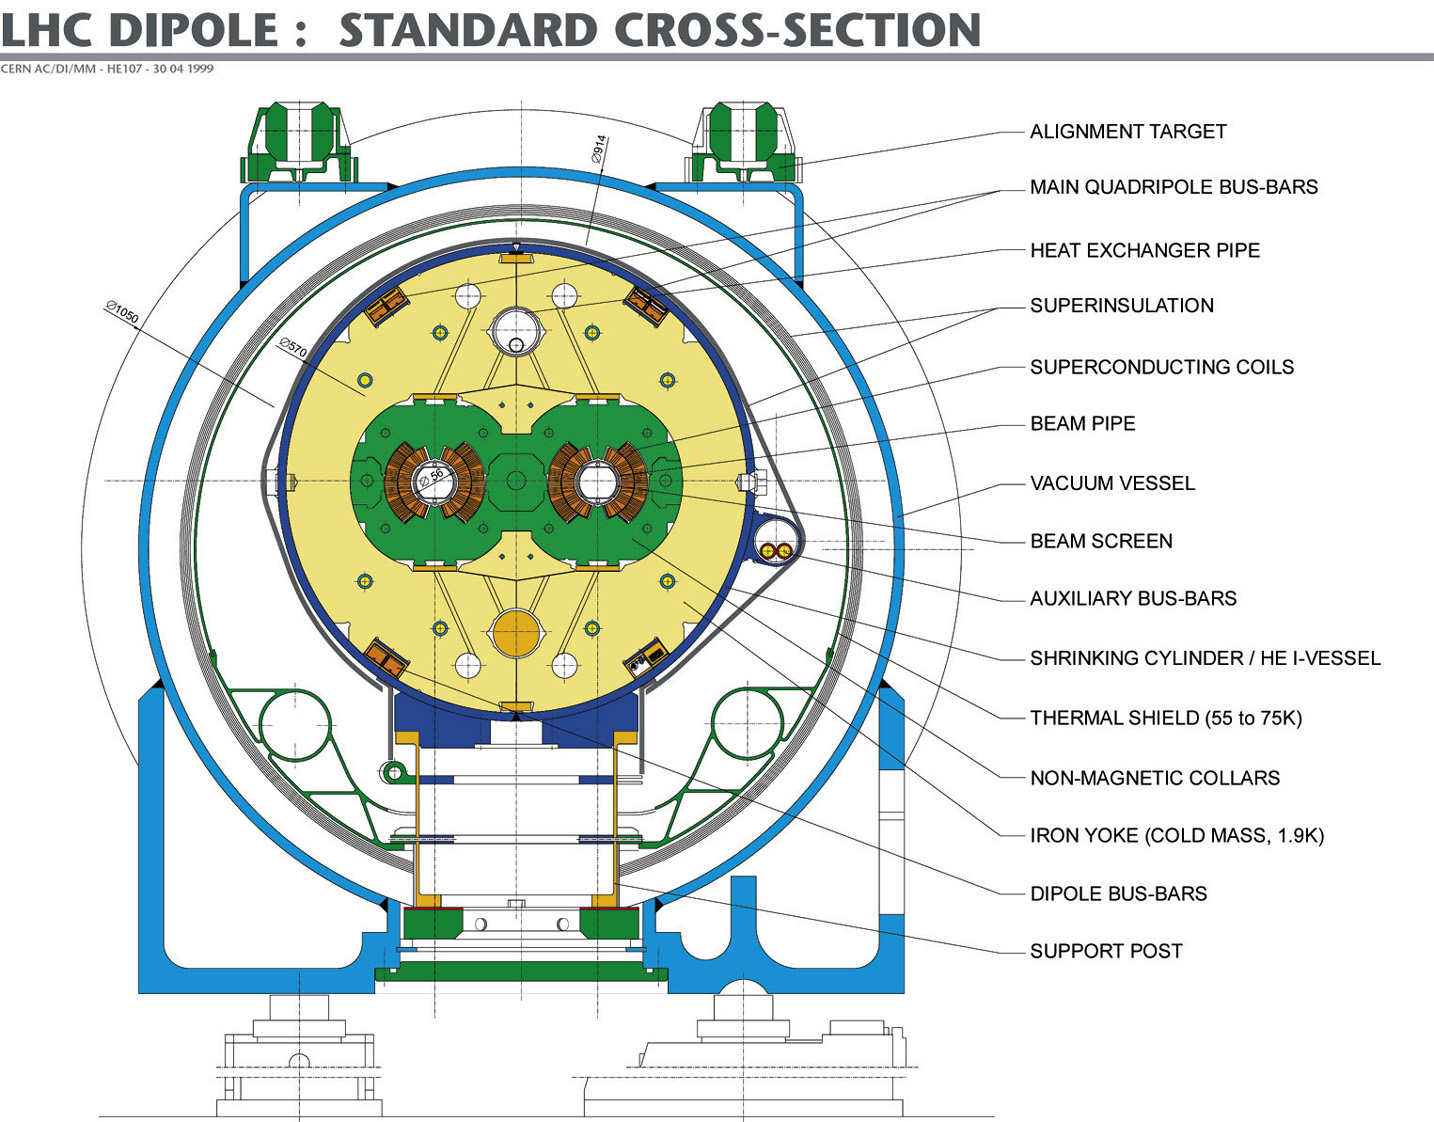
\includegraphics[width=0.7\textwidth]{lhcdipole}
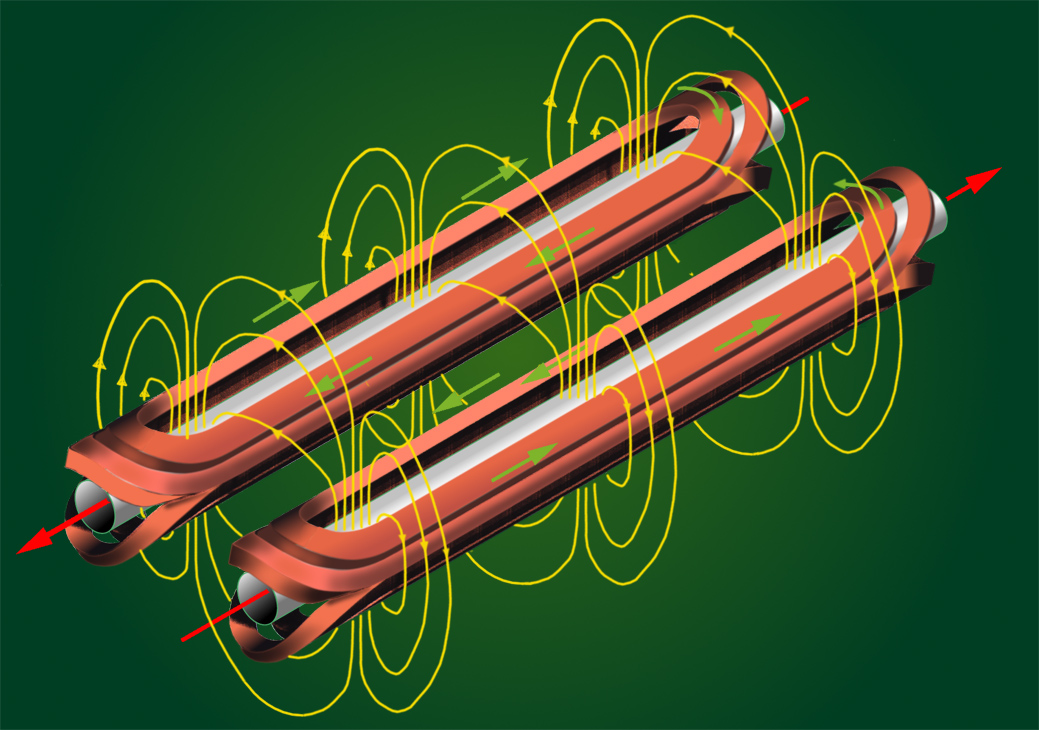
\includegraphics[width=6.0cm,height=4cm]{lhc_dipole2}
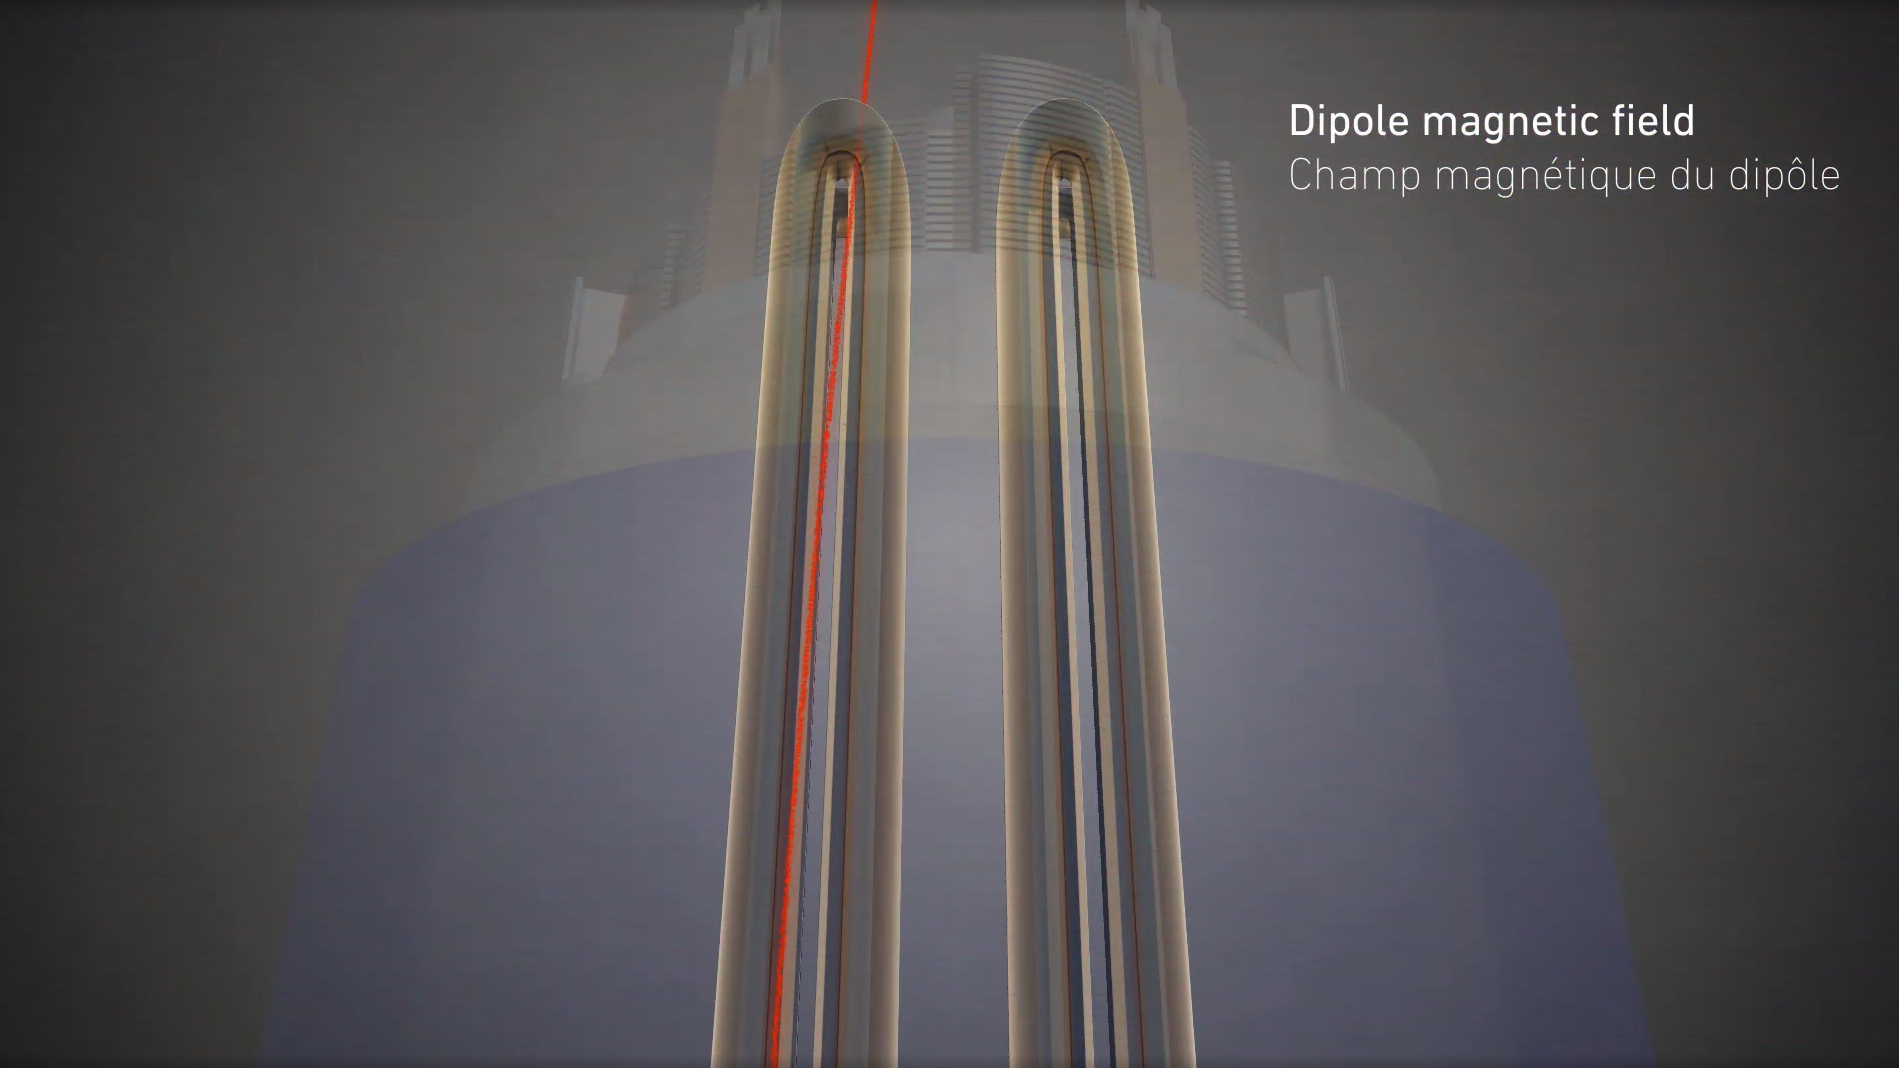
\includegraphics[width=6.0cm,height=4cm]{beam_dev}
\caption [LHC dipole magnet.]{Top: LHC dipole magnet transversal view; cooling, shielding and mechanical support are indicated. Bottom left: Magnetic field generated by the dipole magnets; note that the direction of the field inside one beam pipe is opposite with respect to the other beam pipe which guarantee that both proton beams are curved in the same direction towards the ceneter of the ring. The effect of the dipole magnetic field on the proton beam is represented in the bottom right side \cite{lhc_dipole, dipole_field,video}.}\label{fig:lhcdipole}
\end{figure}

\noindent Protons in the arc sections of LHC feel a centripetal force exerted by the dipole magnets which is perpendicular to the beam trajectory; The magnitude of magnetic field needed can be found assuming that protons travel at $v \approx c$, using the standard values for proton mass and charge and the LHC radius, as
\beqn
F_m=\frac{mv^2}{r}=qBv \quad \to B=8.33 T
\eeqn
\noindent wich is about 100000 times the Earth's magnetic field. A representation of the magnetic field generated by the dipole magnets is shown in the bottom left side of figure \ref{fig:lhcdipole}. The bending effect of the magnetic field on the proton beam is shown in the bottom right side of figure \ref{fig:lhcdipole}. Note that the dipole magnets are not curved; the arc section of the LHC ring is composed of straight dipole magnets of about 15 m. In total there are 1232 dipole magnets along the LHC ring.

\noindent In addition to bending the beam trajectory, the beam has to be focused so it stays in side the beam pipe. The focusing is performed by quadrupole magnets installed in another straight section; in total 858 quadrupole magnets are installed along the LHC ring. Other effects like electromagnetic interaction among bunches, interaction with electron clouds from the beam pipe, gravitational force on the protons, differences in energy among protons in the same bunch, among others, are corrected using sextupole and other magnetic multipoles.     

\noindent The two proton beams inside the LHC ring are made of bunches with a cylindrical shape of about 7.5 cm long and about 1 mm in diameter; when bunches are close to the collision point (CP), the beam is focused up to a diameter of about 16 $\mu$m in order to maximize the luminosity (L) defined as the number of collisions per unit area and per second. Luminosity can be calculated using

\beqn
L=fn\frac{N_1 N_2}{4\pi \sigma_x\sigma_y}
\eeqn

\noindent where f is the revolution frecuency, n is the number of bunches per beam,  $N_1$ and $N_2$ are the number of protons per bunch,  $\sigma_x$ and $\sigma_y$ are the gaussian transverse sizes of the bunches. Using

\begin{align}
  f=&\frac{v}{2\pi r_{LHC}}\approx\frac{3\times10^8m/s}{27km}\approx 11.1 kHz,\nonumber \\
  n=&2808\nonumber \\ 
  N_1=&N_2=1.5\times 10^{11}\nonumber\\
  \sigma_x=&\sigma_y=16\mu m\nonumber
\end{align}
\beqn
L= 1.28\times 10^{34} cm^{-2}s^{-1}
\eeqn

\noindent Luminosity is a fundamental aspect for LHC given that the bigger luminosity, the bigger number of collisions, which means that for processes with a very small cross section the number of expected occurrencies is increased and so the chances of being detected. The integrated luminosty collected by the CMS experiment during 2016 is shown in figure \ref{fig:lumi}; the data analized in this thesis corresponds to an integrated luminosity of 35.9 fb$^{-1}$ at $\sqrt{s}=13$ TeV.

\noindent A way to increase L is increasing the number of bunches in the beam. Currently, the separation between two consecutive bunches in the beam is 7.5 m which corresponds to a time separation of 25 ns. In the full LHC ring the allowed number of bunches is $n=27km/7.5m=3600$; however, there are some gaps in the bunch pattern intended for preparing the dumping and injection of the beam, thus, the proton beams are composed of 2808 bunches. 

\begin{figure}[!h]
\centering
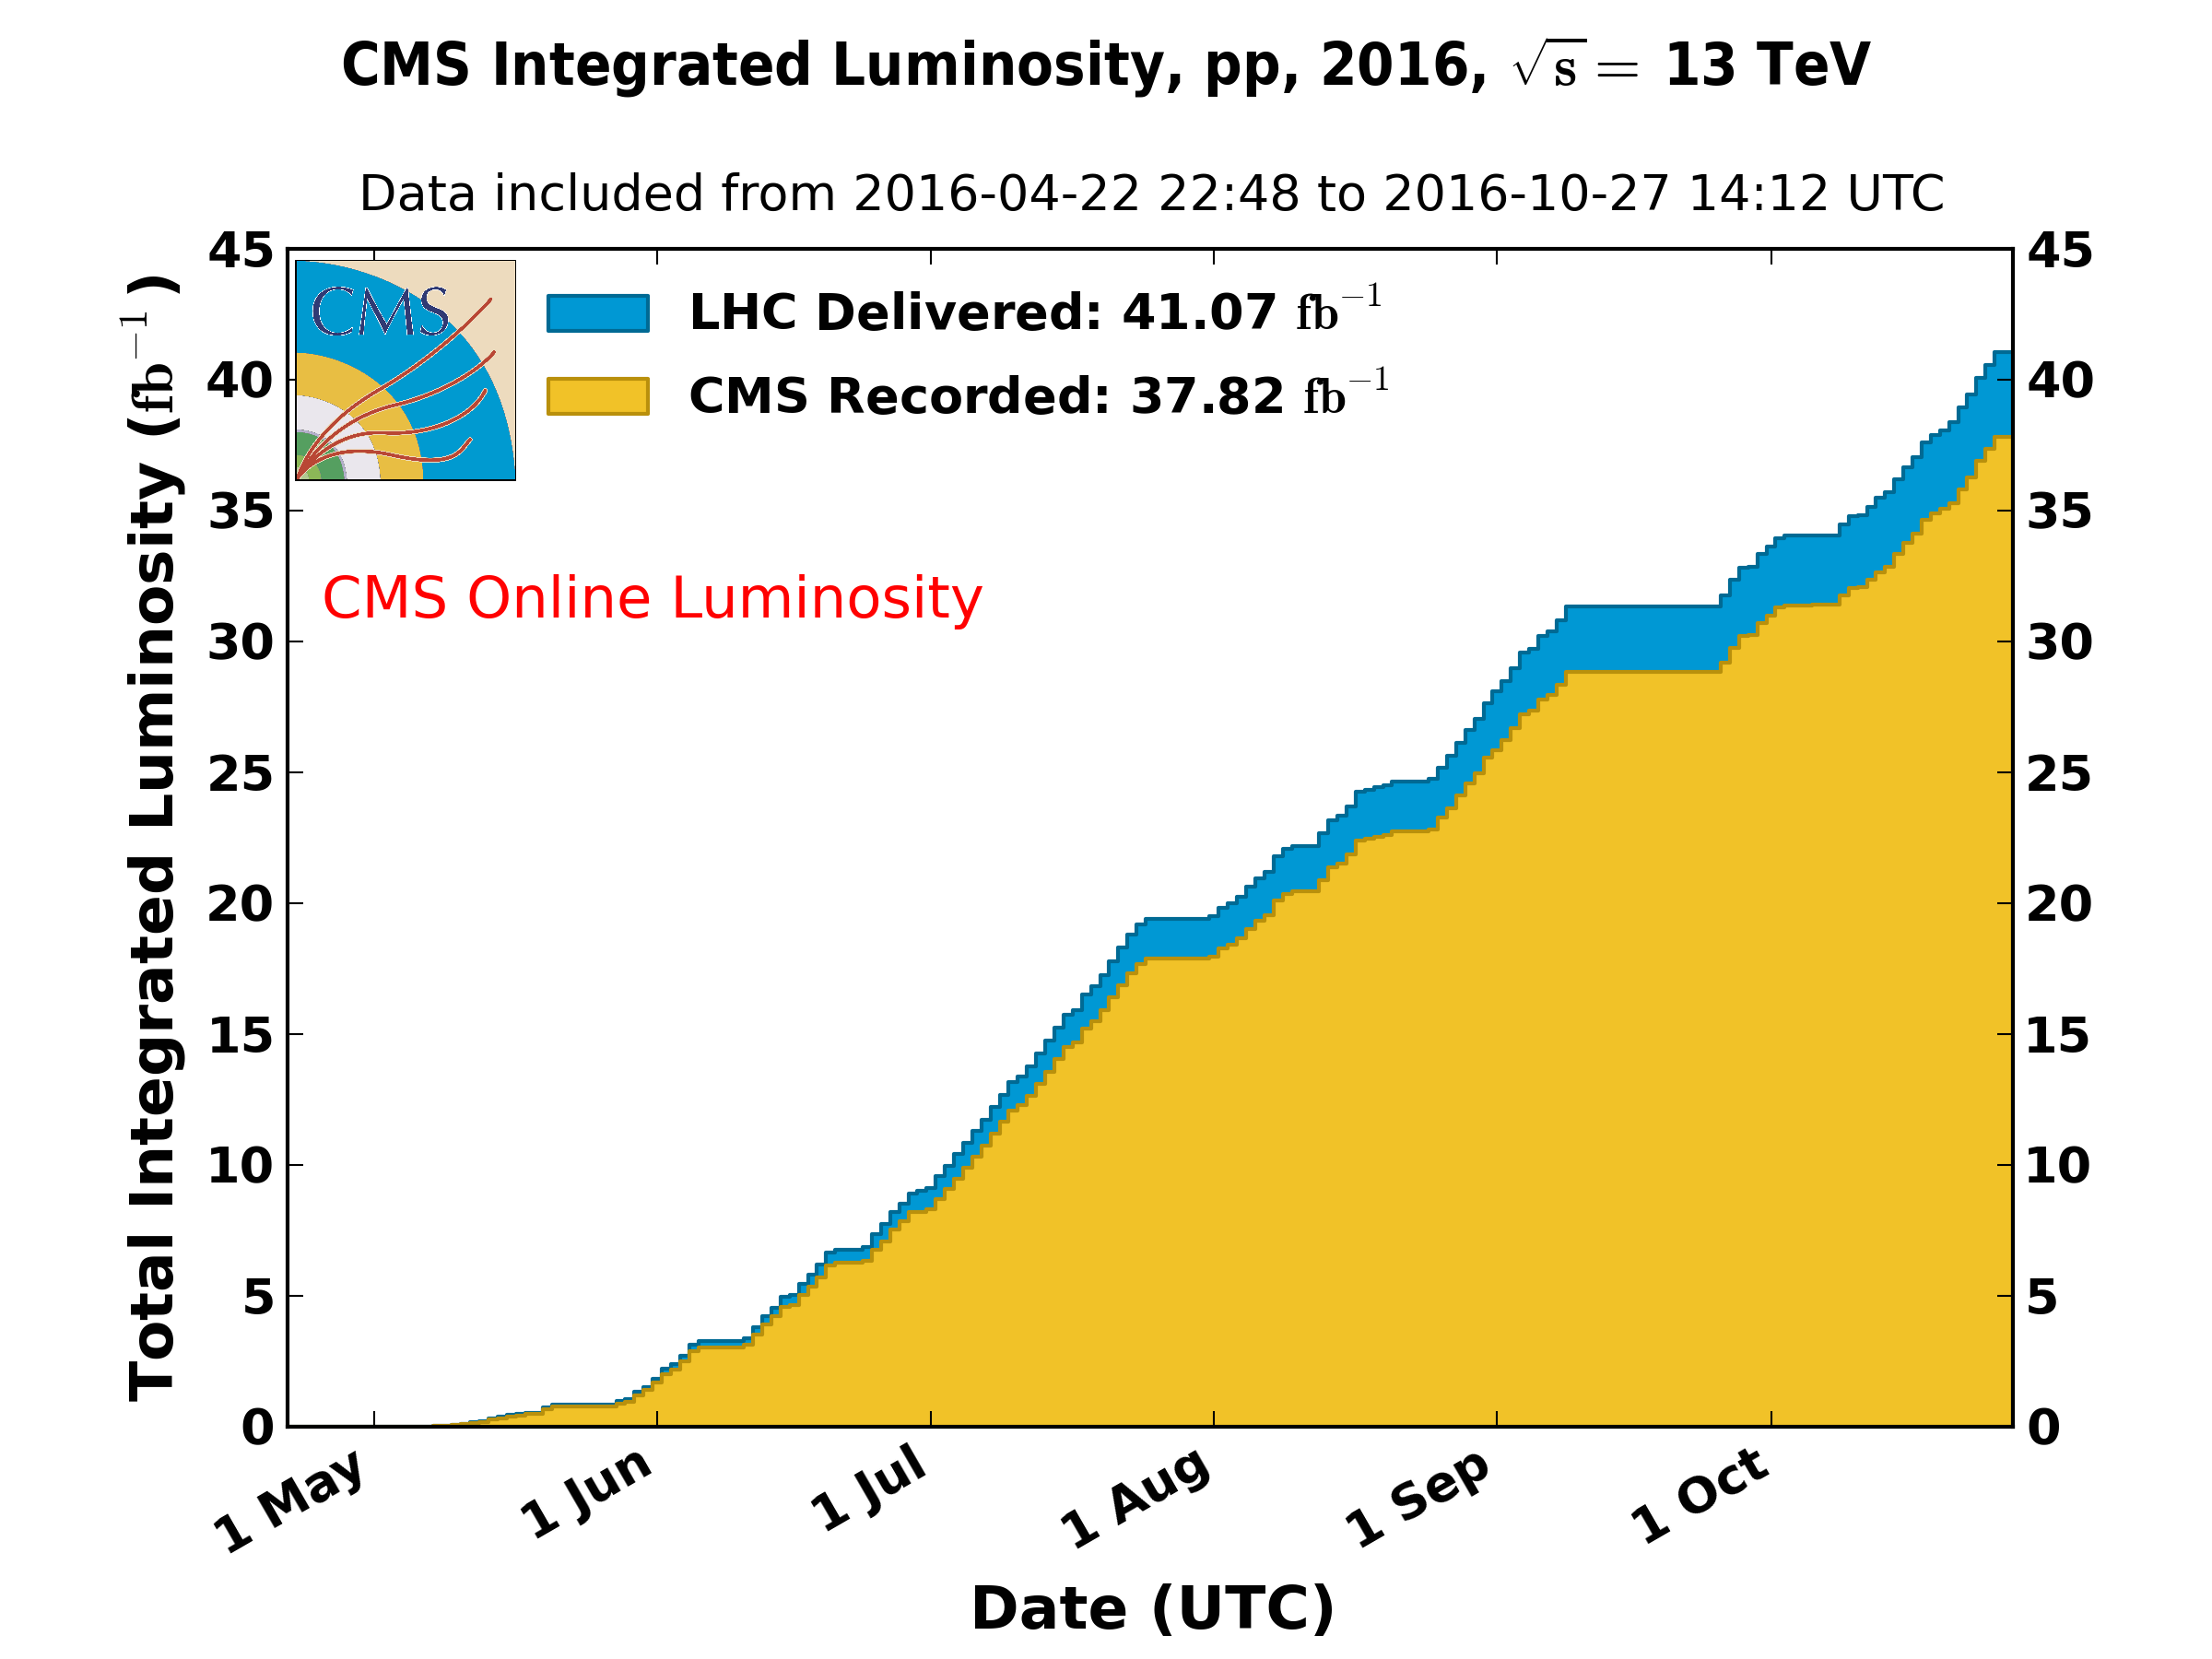
\includegraphics[width=0.7\textwidth]{int_lumi_2016_cms}
\caption [2016 CMS Integrated luminosity]{Integrated luminosity delivered by LHC and recorded by CMS during 2016. The difference between the delivered and the recorded luminosities is due to fails and issues occured during the data taking in the CMS experiment\cite{lumi}.}\label{fig:lumi}
\end{figure}

\noindent Once the proton beams reach the desired energy, they are brought to cross each other producing proton-proton collisions. The bunch crossing happens in precise places where the four LHC experiments are located, as seen in figure \ref{fig:lhc_layout} left. In 2008, the first set of collisions involved protons with $\sqrt{s}=7$ TeV; the energy was increased to 8 TeV in 2012 and to 13 TeV in 2015.

\noindent CMS and ATLAS experiments, which are multi-purpose experiments, are enabled to explore physics in any of the collision modes. LHCb experiment is optimized to explore botom quark physics, while ALICE is optimized for heavy ion collisions searches; TOTEM and LHCf are dedicated to forward physics studies; MoEDAL (not indicated in the figure) is intended for monopoles or massive pseudo stable particles searches.

\begin{figure}[!h]
\centering
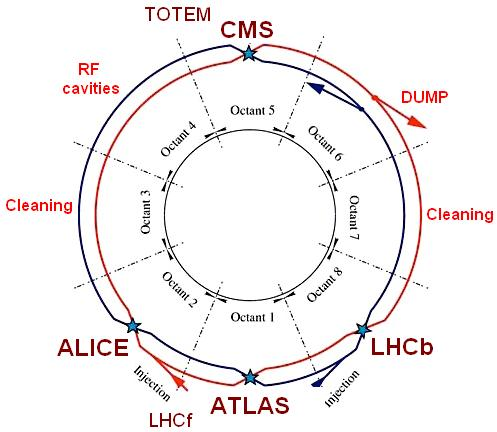
\includegraphics[width=0.55\textwidth]{lhc_layout}
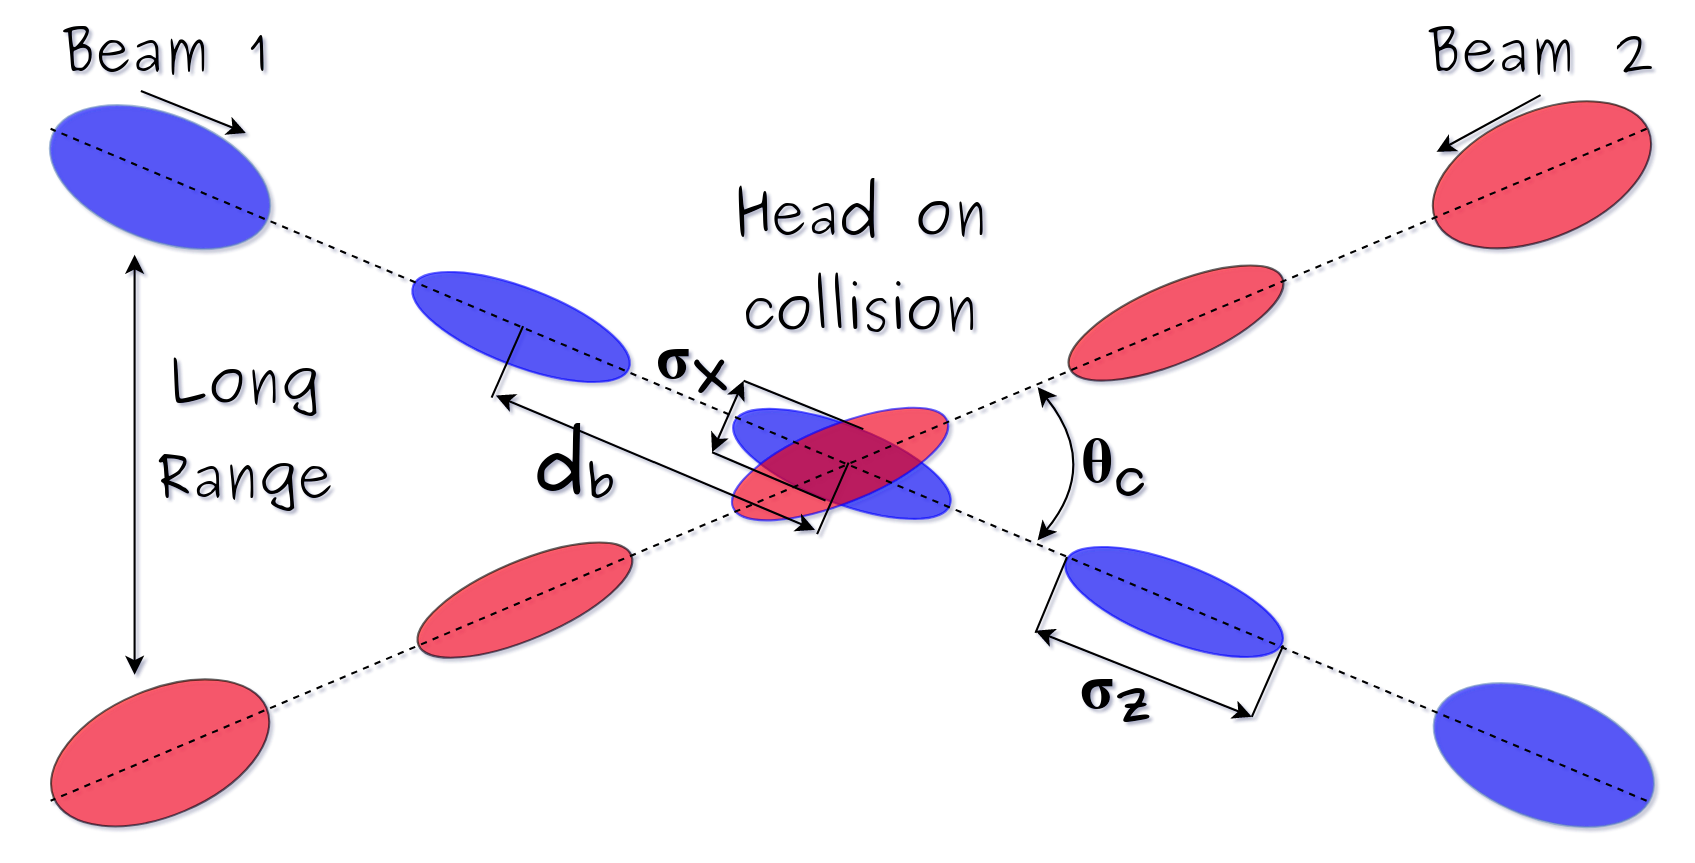
\includegraphics[width=0.4\textwidth]{bcross}
\caption [LHC interaction points]{Left: LHC interaction points. Bunch crossing occurs where the LHC experiments are located \cite{lhc_layout}. Sections indicated as cleaning are dedicated to collimate the beam in order to protect the LHC ring from collisions with protons in very spreaded bunches. Right: bunch crossing scheme. Since the bunch crossing is not perfectly head-on, the luminosity is reduced in a factor of 17\%.}\label{fig:lhc_layout}
\end{figure}

\noindent At the CP there are two interesting details that need to be addressed. The first one is that the bunch crossing does not occur head-on but at a small crossing angle (280 $\mu$rad in CMS and ATLAS) as shown in the right side of figure \ref{fig:lhc_layout}, affecting the overlapping between bunches; the consecuence is a reduction of about 17\% in the luminosity. The second one is occurence of multiple pp collisions in the same bunch crossing; this effect is called pile-up (PU). A fairly simple estimation of the PU follows from estimating the probability of collision between two protons, one from each of the bunches in course of collision; it depends roughly on the ratio of proton size and the cross section of the bunch in the interaction point, \ie,
\beqn
P(pp-collision) \sim \frac{d_{proton}^2}{\sigma_x\sigma_y}=\frac{(1 fm)^2}{(16\mu m)^2} \sim 4\times10^{-21}
\eeqn
\noindent however, there are $N=1.15\times 10^{11}$ protons in a bunch, thus the estimated number of collisions in a bunch crossing is

\beqn
PU= N^2*P(pp-collision)\sim 50  \textrm{  pp-collision per bunch crossing},
\eeqn

\noindent about 20 of those pp collisions are inelastic. Each collision generates a vertex, but only the most energetic is considered as a primary vertex; the rest are considered as PU vertices. A simulation of a multiple pp collision event in a bunch crossing at CMS is showed in figure\ref{fig:pu}. Unstable particles outgoing from the primary vertex will eventually decay; this decay vertex is knon as a secondary vertex.      

\begin{figure}[!h]
\centering
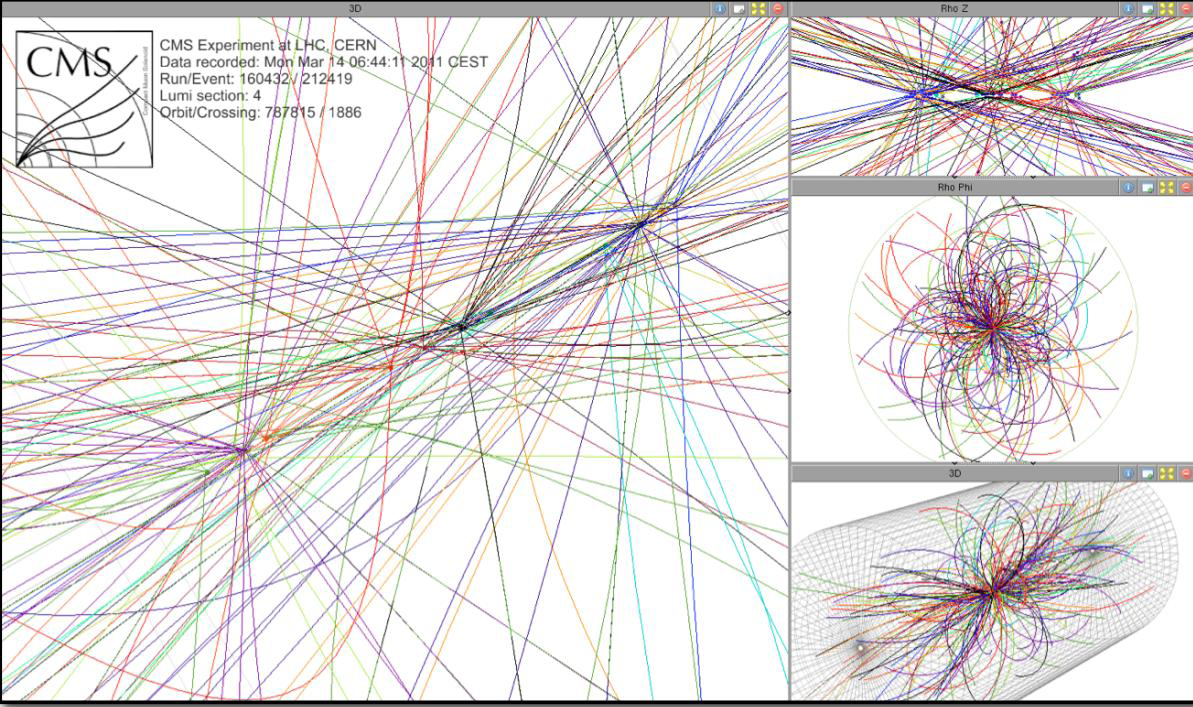
\includegraphics[width=0.65\textwidth]{pu}
\caption [Multiple pp collision bunch crossing at CMS.]{Multiple pp collision bunch crossing at CMS. Only the most energetic vertex is considered and the rets are cataloged as PU vertices \cite{}. }\label{fig:pu}
\end{figure}

\noindent When the beams are exhausted, \ie the number of protons in the bunches is reduced beyond a limit, or in case of emergency, the beams have to be extracted from the beam pipes; the dumping system, in the dump section, perform the extraction safely by directing the beams towards graphite blocks that absorb the beam energy.\\

\noindent Next section present a description of the CMS detector, since it is the detector used to collect the data used in this thesis.


\section{The CMS experiment}

\noindent CMS is a general purpose detector designed to conduct research in a wide range of physics from standard model to new physics like extra dimensions and dark matter. Located at the point 5 in the LHC layout as shown in figure \ref{fig:lep_rfc}, CMS is composed of several detection systems distributed in a cylindrical structure,. In total, CMS weights about 12500 tons in a very compact 21.6 m long and 14.6 m diameter cylinder. It was built in 15 separate sections at the ground level and lowered to the cavern individually to be assembled. A complete and detailed description of the CMS detector and its components is given in reference \cite{cms} on which this section is based in.\\

\noindent Figure \ref{fig:cms} shows the layout of the CMS detector. The design is driven by the requirements on the identification, momentum resolution and unambiguous charge determination of the muons; therefore, a large bending power is provided by the solenoid magnet made of superconducting cable capable to generate a 3.8 T magnetic field. The detection system is composed of (from the innermost to the outermost)

\begin{figure}[!h]
  \centering
  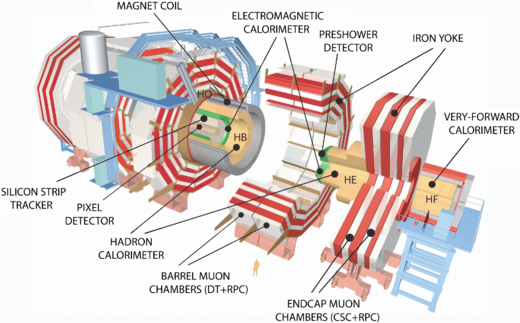
\includegraphics[width=\textwidth]{cms}
  \caption[CMS detector drawing]{CMS detector drawing. The several subdetectors are indicated. The central region of the detector is refferred as the Barrel section while the endcaps are referred as the forward sections. \cite{cms_drawing}.}
  \label{fig:cms}
\end{figure}

\noindent 

\bit
\item Pixel detector.
\item Silicon strip tracker.
\item Preshwoer detector.
\item Electromagnetic calorimeter.
\item Hadronic calorimeter.
\item Muon chambers (Barrel and endcap)
\eit

\noindent The central region of the detector is commonly referred as the barrel section while the endcaps are referred as the forward sections of the detector; thus, each subdetector is composed of a barrel section and a forward section. 


\subsection{Coordinate system}
\noindent The coordinate system used by CMS is centerd in the geometrical center of the detector which is the same as the CP as shown in figure\ref{fig:coord}. The $z$-axis is parallel to the beam direction, while the $Y$-axis pointing vertically upward, and the $X$-axis pointing radially inward toward the center of the LHC.

\begin{figure}[h!]
  \centering
  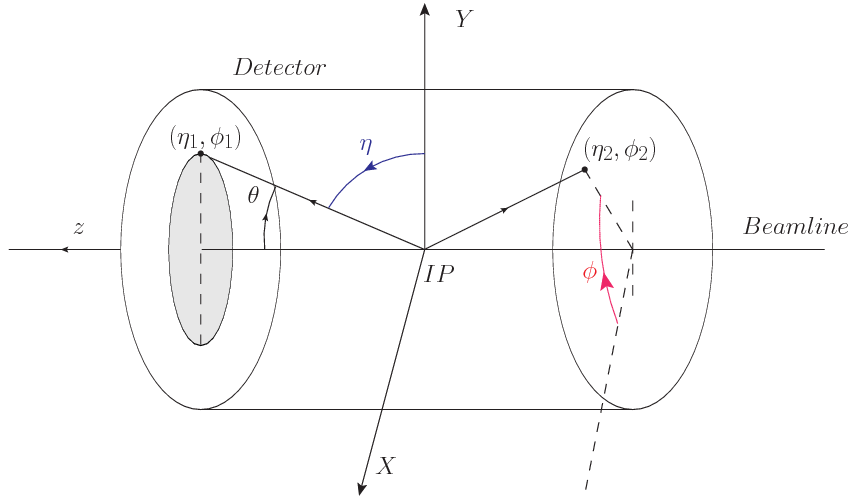
\includegraphics[scale=0.4]{coord}
  \caption[CMS coordinate system]{CMS coordinate system.}
  \label{fig:coord}
\end{figure}

\noindent In addition to the common cartesian and cylindrical coordinate systems, two coordinates are of particular utility in particle physics: rapidity($y$) and pseudorapidity($\eta$), defined in conection to the polar angle $\theta$, energy and longitudinal momentum component (momentum along the $z$-axis) according to

\beqn
y=\frac{1}{2}ln\frac{E+p_z}{E-p_z} \qquad \eta=-ln \left(tan\frac{\theta}{2}\right)
\label{eqn:eta}
\eeqn

\noindent Rapidity is related to the angle between the $XY$-plane and the direction in which the products of a collision are emitted; it has the nice property that the difference between the rapidities of two particles is invariant with respect to Lorents boosts along the $z$-axis. Thus, data analysis becomes more simple when based in rapidity; however, it is not simple to measure the rapidity of higly relativistic particles, as those produced after pp collisions. Under the highly relativistic motion approximation $y$ can be rewritten in terms of the polar angle, arriving to the conclusion that rapidity is approximately equal to the pseudorapidity defined above, \ie $y\approx\eta$. Note that $\eta$ is easier to measure that $y$ given the direct relationship between the former and the polar angle. Angular distance between two objects in the detector ($\Delta R$) is defined in terms of their coordinates $(\eta_1,\phi_1)$, $(\eta_2,\phi_2)$ as
\beqn
\Delta R = \sqrt{(\Delta\eta)^2 - (\Delta\phi)^2 }
\eeqn

\subsection{Pixels detector}

\noindent  The CMS tracking system is designed to provide a precise measurement of the trajectory followed by the charged particles created after the pp collisions as; also, the precise reconstruction of the primary and secondary vertices is expected in an environment where, each 25 ns, the bunch crossing produce about 20 inelastic collisions and about 1000 particles. An increment in the luminosity is ongoing which implies that the PU will increase accordingly. \\

\noindent The pixel detector was replaced during the 2016-2017 year end shut down, due to the increasingly challenging operation conditions like the higher particle flow and more radiation harsh environment among others. The new one is responding as expected, reinforcing its crucial role in the successful way to fullfil the new LHC physics objetives after the discovery of the Higgs boson. The last chapter of this thesis is dedicated to describe my contribution to the `` Forward Pixel Phase 1 upgrade''.\\

\noindent  The current pixel detector is composed of 1856 silicon pixel detector modules organized in four barrel layers in the central region and three disks in the forward region; it is designed to record efficiently and with high precision, up to 10$\mu$m in the $XY$-plane and 20$\mu$m in the $z$-direction, the first four space-points near to the CP region (see figure \ref{fig:pixel_tracker} left side) in the range $|\eta|\leq 2.5$. The first barrel layer is located at a radius of 30 mm from the beamline, while the fourth layer is located at a radius of 160 mm closer to the strip tracker innner barrel layer (see section \ref{sst}) in order to reduce the rate of fake tracks. The high granularity of the detector is represented in its about 123 Mpixels, each of size $100\times150\mu$m$^2$, which is almost twice the channels of the old detector. The transverse momentum resolution of tracks can be measured with a resolution of 1-2\% for muons of $p_T=100$ GeV. \\

\begin{figure}[h!]
  \centering
  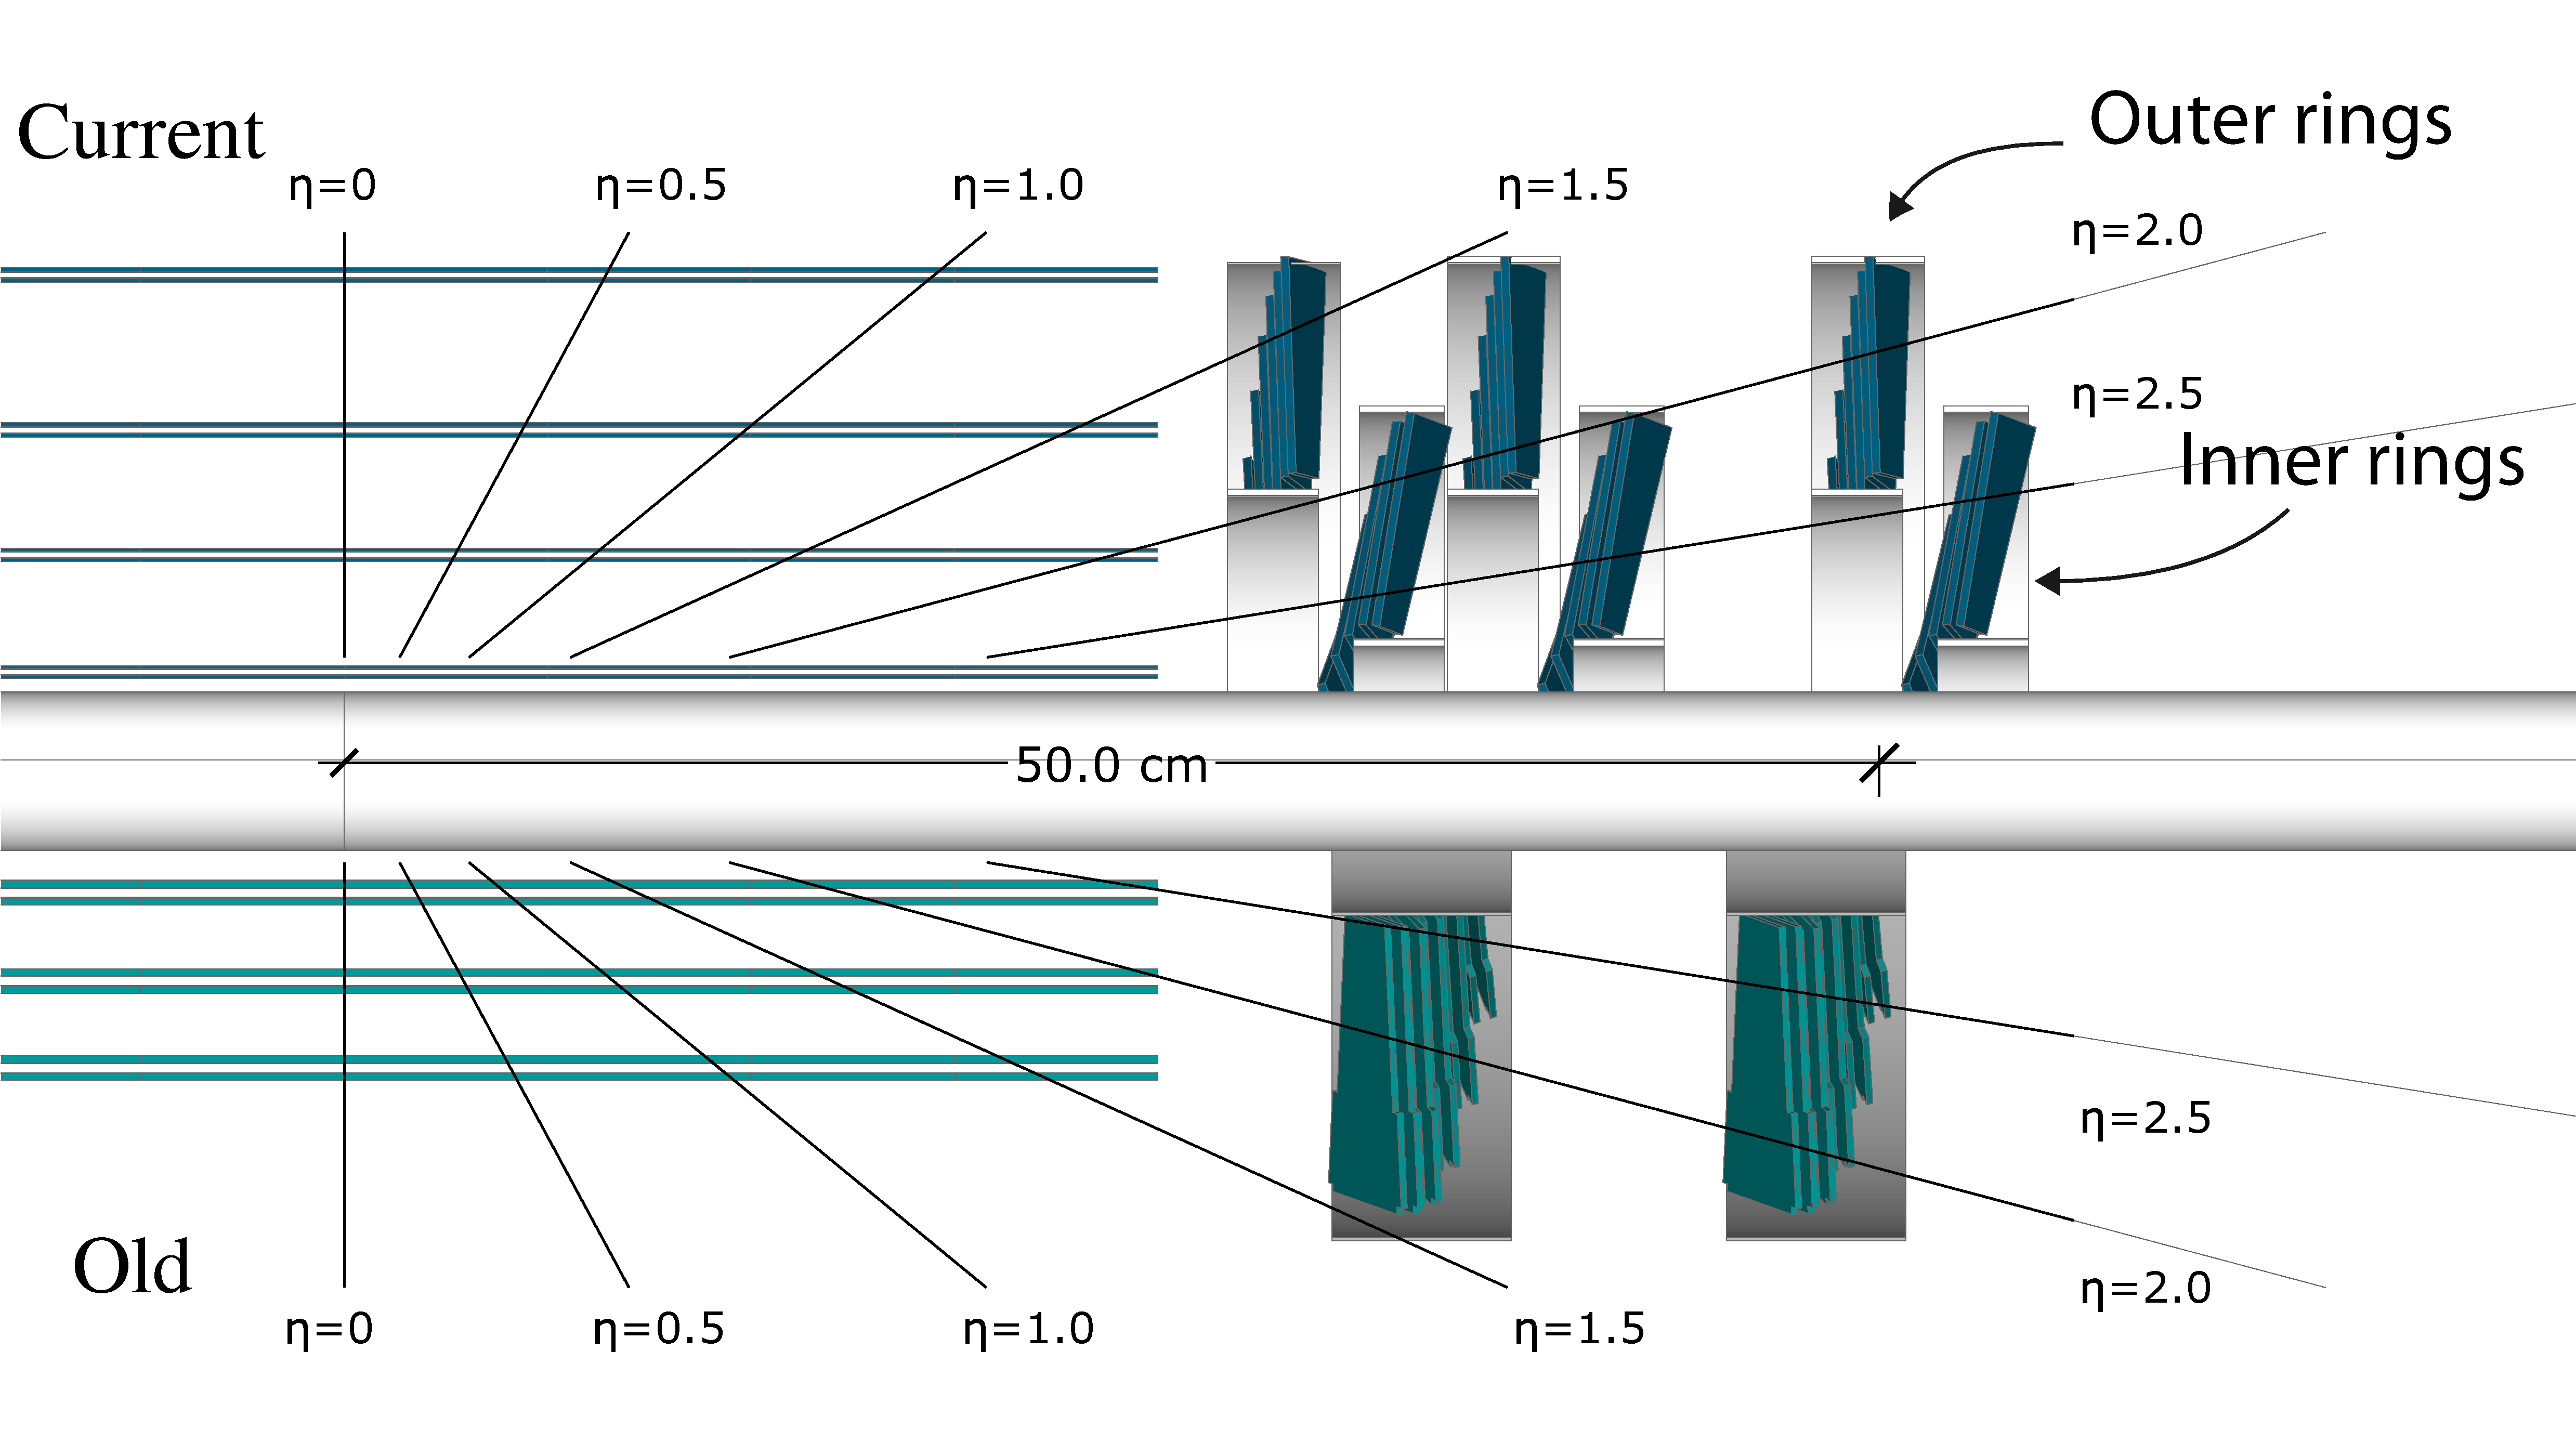
\includegraphics[width=9.5cm]{fpix1}
  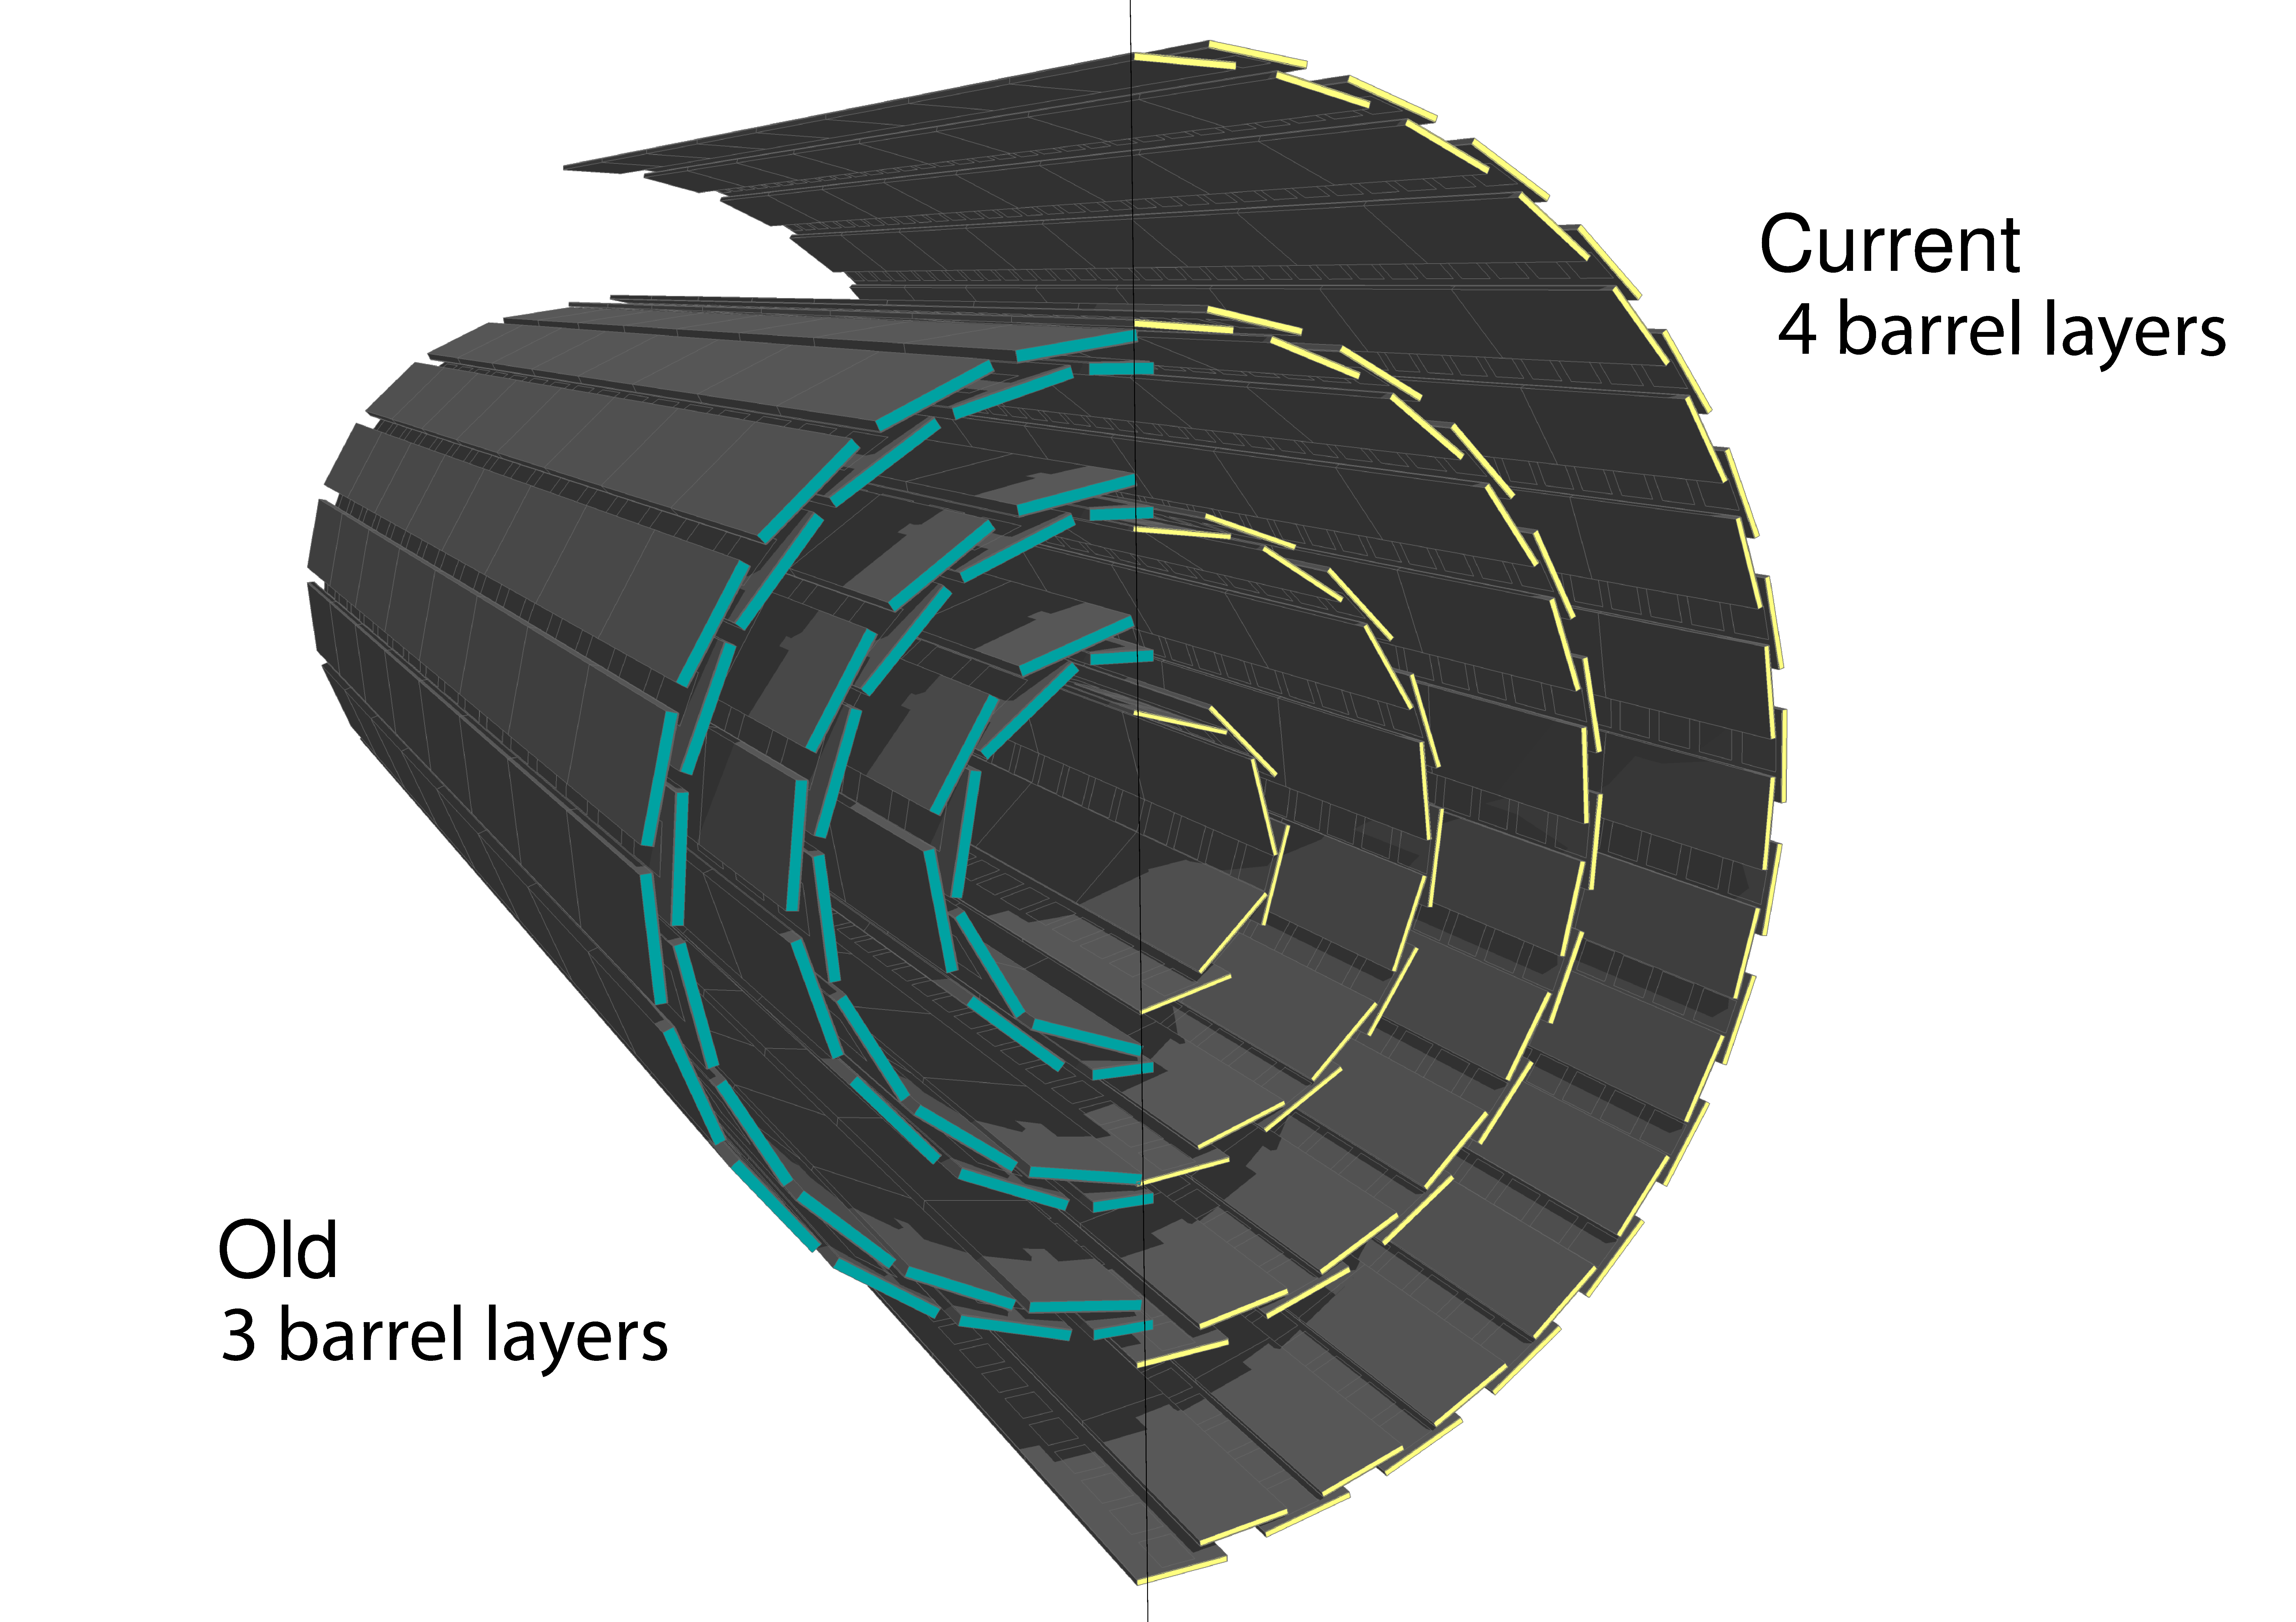
\includegraphics[width=5.5cm]{bpix1}
  \caption[CMS pixel detector schematic view.]{CMS pixel detector schematic view. Left: layout comparing the layers and disks in the old and current pixel detectors. Right: Transverse-oblique view comparing the pixel barrel layers in the two \cite{pix_tdr}.}
  \label{fig:pixel_tracker}
\end{figure}

\noindent Some of the improvements with respect to the previous pixel detector include a higher average tracking efficiency and lower average fake rate as well as higher track impact parameter resolution which is fundamental in order to increase the efficiency in the identification of jets originating from b quarks (b-tagging). A significant source of improvement comes from the overall reduction in the material budget of the detector which results in less photon conversions and less multiple scattering from charged particles.    

\subsection{Silicon strip tracker}\label{sst}
\begin{figure}[h!]
  \centering
  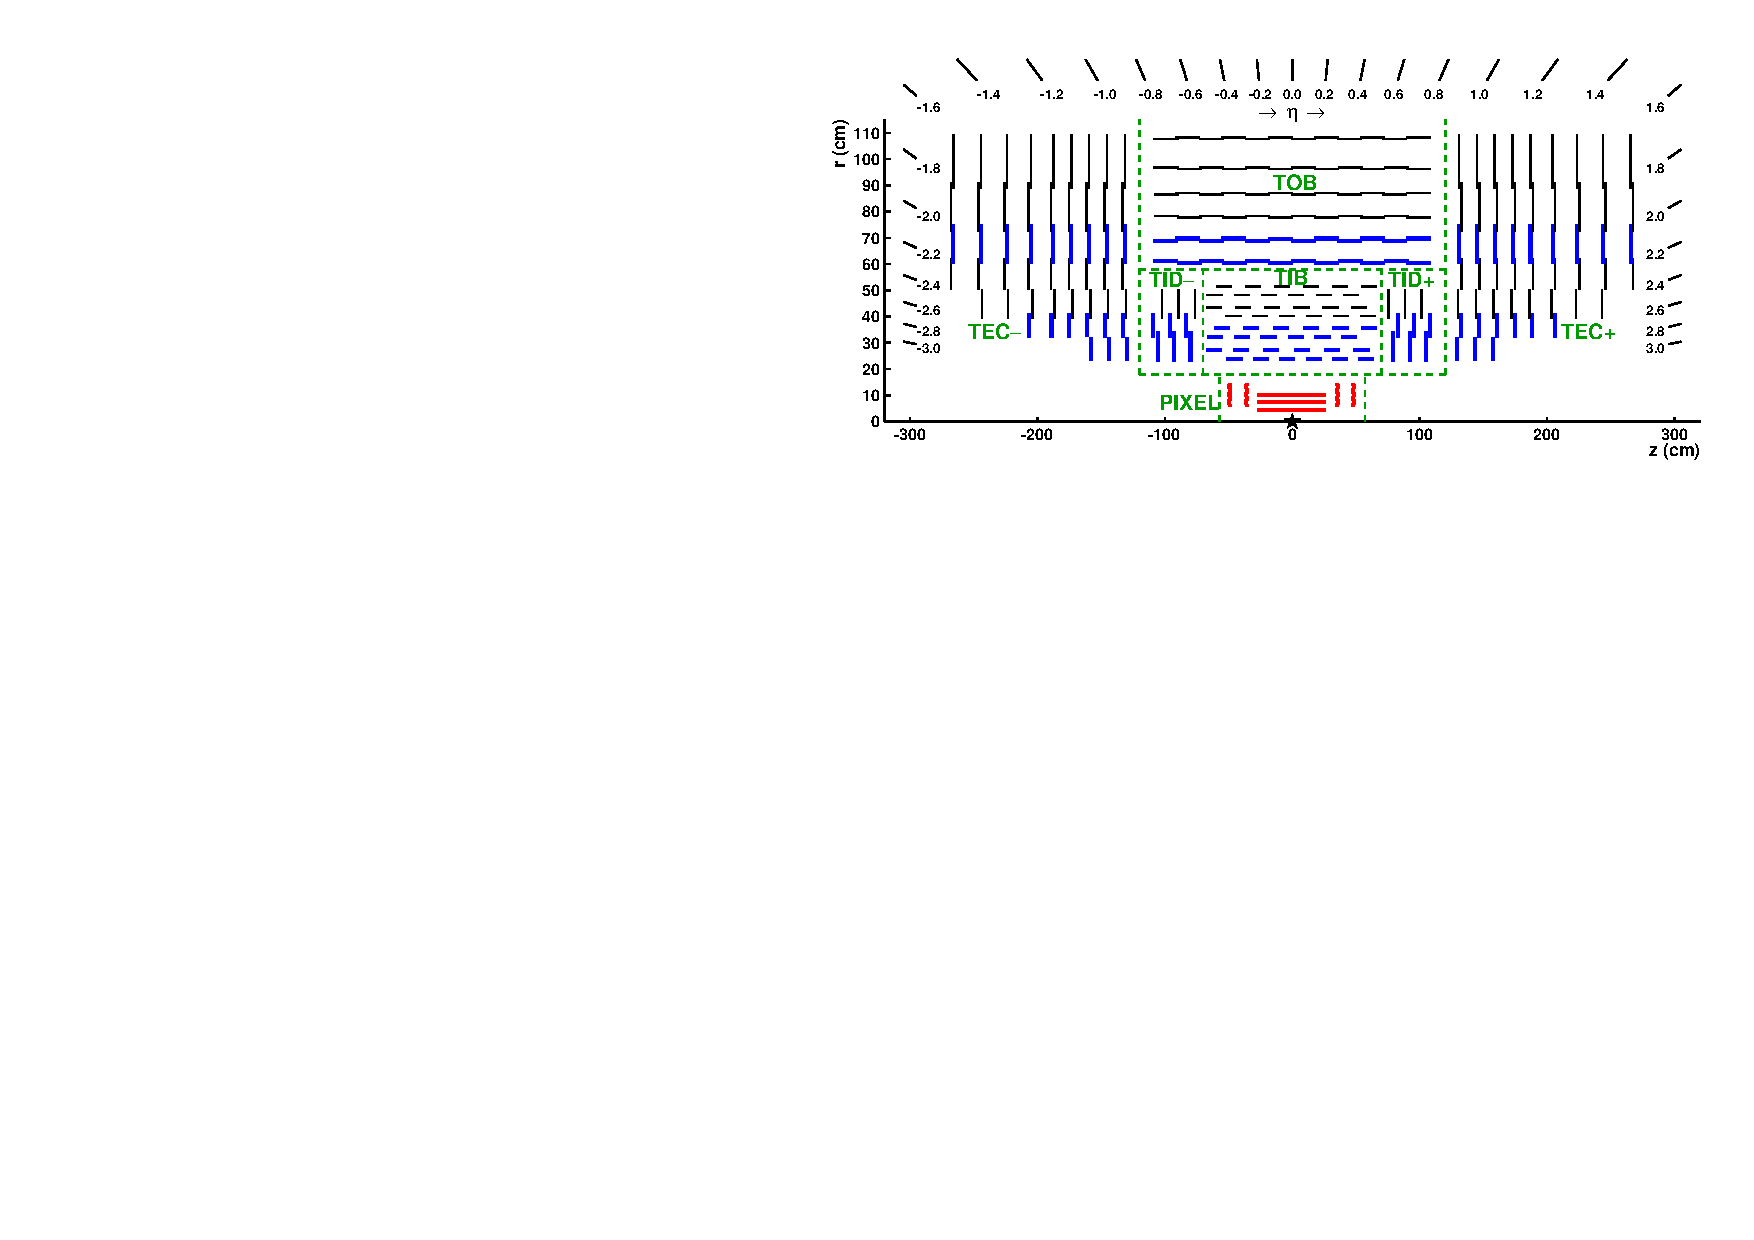
\includegraphics[width=12cm]{sst1}
  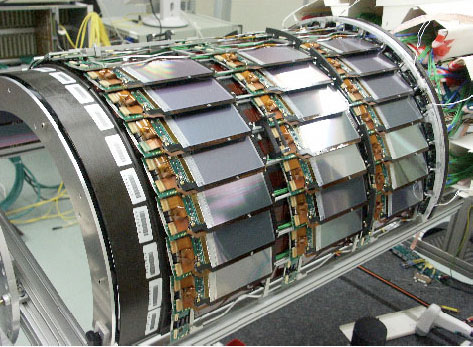
\includegraphics[width=6cm,height=4cm]{tib}
  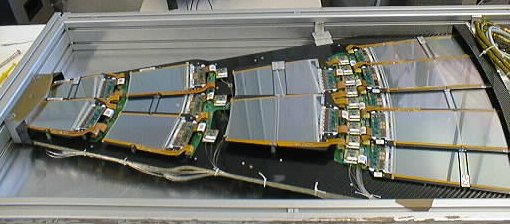
\includegraphics[width=6cm,height=4cm]{tec}
  %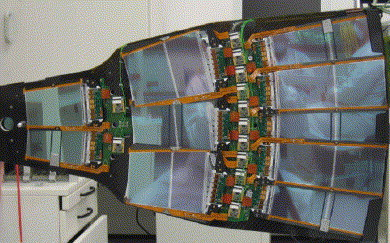
\includegraphics[width=6cm]{tec2}
  \caption[SST Schematic view.]{Top: CMS Siicon Strip Tracker (SST) schematic view. The SST is composed of the tracker inner barrel (TIB), the tracker inner disks (TID), the tracker outer barrel (TOB) and the tracker endcaps (TEC). Each part is made of silicon strip modules; the modules in blue represent two modules mounted back-to-back and rotated in the plane of the module by a stereo angle of 120 mrad in order to provide a 3-D reconstruction of the hit positions. Bottom: pictures of the TIB (left) and TEC (right) modules \cite{sst,tib,tec}.}
  \label{fig:sst}
\end{figure}

\noindent The silicon strip tracker (SST) is the second stage in the CMS tracking system . The top side of figure \ref{fig:sst} shows a schematic of the SST. The inner tracker region is composed of the tracker inner barrel (TIB) and the tracker inner disks (TID) covering the region $r<55$ cm and $|z|<118$ cm. The TIB is composed of 4 layers while the TID is composed of 3 disks at each end. The silicon sensors in the inner tracker are 320 $\mu$m thick, providing a resolution of about 13-38 $\mu$m in the $r\phi$ position measurement. \\

\noindent The modules indicated in blue in the schematic view of figure \ref{fig:sst} are two modules mounted back-to-back and rotated in the plane of the module by a ``stereo'' angle of 100 mrad; the hits from these two modules, known as ``stereo hits'', are combined to provide a measurement of the second coordinate (z in the barrel and r on the disks) allowing the reconstruction of hit positions in 3-D.\\ 

\noindent The outer tracker region is composed of the tracker outer barrel (TOB) and the tracker endcaps (TEC). The 6 layers of the TOB offers coverage in the region $r>55$ cm and $|z|<118$ cm, while the 9 disks of the TEC cover the region $124<|z|<282$ cm. The resolution offered by the outer tracker is about 13-38 $\mu$m in the $r\phi$ position measurement. The inner four TEC disks use silicon sensors 320 $\mu$m thick; those in the TOB and the outer three TEC disks use silicon sensors of 500 $\mu$m thickness. The silicon strips run parallel to the $z$-axis and the distance between strips varies from 80 $\mu$m in the inner TIB layers to 183 $\mu$m in the inner TOB layers; in the endcaps the wedge-shaped sensors with radial strips, whose pitch range between 81 $\mu$m at small radii and 205 $\mu$m at large radii.\\ 

\noindent The whole SST has 15148 silicon modules, 9.3 million silicon strips and cover a total active area of about 198 m$^2$ 

\subsection{Electromagnetic calorimeter}
\begin{figure}[h!]
  \centering
  \includegraphics[scale=0.2]{ecal}
  \includegraphics[width=6cm,height=4cm]{ecal_module}
  \includegraphics[width=6cm,height=4cm]{ecal_crystal} 
  \caption[CMS ECAL schematic view]{Top: CMS ECAL schematic view. Bottom: Module equipped with the crystals (left); ECAL crytal(right).}
  \label{fig:ecal}
\end{figure}

\noindent The CMS electromagnetic calorimeter (ECAL) is designed to measure the energy of electrons and photons. It is composed of 75848 lead tungstate crystals which has a short radiation length (0.89 cm) and fast response given that 80\% of the light is emmited within 25 ns; however, they are combined with Avalanche photodiodes (APDs) as photodetectors given that crytals themself have a low light yield (30$\gamma$/MeV). An schematic view of the ECAL is shown in figure \ref{fig:ecal}.\\

\noindent Energy is measured by absorbing electrons and photons which generates an electromagnetic ``shower'', as seen in bottom right picture of the figure\ref{fig:ecal}. The ECAL barrel (EB) cover the region $|\eta|$ < 1.479, using crystals of depth of 23 cm and  $2.2\times 2.2$ cm$^2$ transverse section. 

\noindent The ECAL endcap (EE) cover the region 1.479 < $|\eta|$ < 3.0 using crystals of depth 22 cm and transverse section of $2.86\times2.86$ cm$^2$; the photodetectors used are vacuum phototriodes (VPTs). Each EE is divided in two structures called ``Dees''.\\

\noindent In front of the EE, it is installed the preshower detector (ES) which covers the region $1.653 < |\eta| < 2.6$. The ES provides a precise measurement of the position of electromagnetic showers, which allows to distinguish electrons and photons signals from $\pi^0$ decay signals. The ES is composed of a layer of lead absorber followed by a layer of plastic scintillators

\subsection{Hadronic calorimeter}

\begin{figure}[h!]
  \centering
  \includegraphics[scale=0.3]{hcal}\\
  \includegraphics[width=3.5cm,height=4.5cm]{hb}
  \includegraphics[width=4.5cm,height=4.5cm]{hb2}
  \includegraphics[width=4.5cm,height=4.5cm]{ho1} 
  \caption[CMS HCAL schematic view]{Top: CMS HCAL schematic view, the colors indicate the layers that are grouped into the same readout channels. Bottom: picture of a section of the HB; the absorber material is the golden region and scintillators are placed in between the absorber material (left and center). Schematic view of the HO (right).\cite{hcal,hb} }
  \label{fig:hcal}
\end{figure}

\noindent Hadrons are not absorbed by the ECAL but by the hadron calorimeter (HCAL), which is made of a combination of alternating brass absorber and silicon photomultiplier(SiPM) layers; therefore, particles passing through the scintillator material produce showers, as in the ECAL, as a result of the inelastic scattering of the hadrons with the detector material. Since the particles are not absorbed in the scintillator, their energy is sampled; therefore the total energy is not measured but stimated, which reduce the resolution of the detector. Brass was choosen as the absorber material due to its short interaction lenght ($\lambda_I=16.42$cm) and its non-magnetivity. Figure \ref{fig:hcal} shows an schematic view of the CMS HCAL.\\

\noindent The HCAL is divided in four sections; the Hadron Barrel (HB), the Hadron Outer (HO), the Hadron Endcap (HE) and the Hadron Forward (HF) sections. The HB cover the region $0<|\eta|<1.4$, while the HE covers the region $1.3<|\eta|<3.0$. The HF, made of quartz fiber scintillator and steel as absorption material, covers the forward region $3.0<|\eta|<5.2$. Both the HB and HF are located inside the solenoid. The HO is placed outside the magnet as an additional layer of scintillators with the purpose of measure the energy tails of particles passing through the HB and the magnet (see figure \ref{fig:hcal} top and bottom right) . The upgrades made to the HCAL during the technical stop 2016-2017 consisted in the replacement of the phototransducers, improving the efficiency.

\subsection{Superconducting solenoid magnet}

\begin{figure}[h!]
  \centering
  \includegraphics[scale=0.38]{magnet}
  \includegraphics[scale=0.4]{yoke2}
  %\includegraphics[scale=0.4]{yoke1} 
  \caption[CMS solenoid magnet]{Artistic representation of the CMS solenoid magnet(left). The magnet is supported on an iron yoke (right) which also serves as the house of the muon detector and as mechanical support for the whole CMS detector \cite{yoke2}.}
  \label{fig:yoke}
\end{figure}

\noindent The superconducting magnet installed is the CMS detector is designed to provide an intense and highly uniform magnetic field in the central part of the detector. In fact, the tracking system takes advantage of the bending power of the magnetic field to measure with precision the momentum of the particles that traverse it; the unambiguous determination of the sign for high momentum muons was a driven principle  during the design of the magnet. The magnet has a diameter of 6.3 m, a length of 12.5 m in a cold mass of 220 t; the generated magnetic field reach a strength of 3.8T. Since it is made of Ni-Tb superconducting cable it has to operate at a temperature of 4.7 K by using a helium cryogenic system; the current circulating in the cables reach 18800 A under normal running conditions. The left side of figure \ref{fig:yoke} shows an artistic view of the CMS magnet, while the right side shows a transverse view of the cold mass where the winding structure is visible. \\

\noindent The yoke (see figure \ref{fig:yoke}), composed of 5 barrel wheels and 6 endcap disks made of iron, serves not only as the media for magnetic flux return, but also provides the house for the muon detector sytem and structural stability to the full detector.     

\subsection{Muon system }

\begin{figure}[h!]
  \centering
  \includegraphics[width=10cm,height=6cm]{muon}
  \includegraphics[width=5cm,height=4.55cm]{muon2}
  \caption[CMS Muon system schematic view]{Left: CMS muon system schematic view; Right: one of the yoke rings with the muon DTs and RPCs installed; in the back it is posible to see the muon endcap\cite{muon}. }
  \label{fig:muon_chambers}
\end{figure}

\noindent Muons are the only charged particles able pass through all the CMS detector due to their low ionization energy loss; thus, muons can be separated easily from the high amount of particles produced in a pp collision. Also, muons are expected to be produced in the decay of several new particles; therefore, a good detection of muons was on the leading principles when designing the CMS detector.\\

\noindent The CMS muon detection system is embedded in the return yoke as seen in figure \ref{fig:muon_chambers}. It is composed of three different detector types; the drift tube chambers (DT) are located in the central region $\eta< 1.2$ arranged in four layers of drift chambers filled with an Ar/CO$_2$ gas mixture.\\

\noindent The muon endcaps are made of Cathode strip chambers (CSC) covering the region $\eta< 2.4$ and filled with a mixture of Ar/CO$_2$/CF$_4$. The reason behind using a different detector type lies on the different conditions in the forward region like the high muon rate and high residual magnetic field.\\

\noindent The third type of detector used in the muon system is a set four disks of resistive plate chambers (RPC) working in avalanche mode. The RPCs provide good spatial and time resolutions. The track of $high-p_T$ muon candidate is build combining information from the tracking system and the signal from up to 6 RPCs and 4 DT chambers.
\subsection{trigger system - HLT- L1 }


The
online event selection process (trigger) must reduce the huge rate to about 100 events/s for storage
and subsequent analysis. The short time between bunch crossings, 25 ns, has major implications
for the design of the read-out and trigger systems.


Due to its high segmentation, the pixel detector not only forms high quality seeds for
the track reconstruction algorithm offline, but is also used to do fast tracking online in the high
level trigger (HLT) for primary vertex reconstruction, electron/photon identification, muon
reconstruction, tau identification and b-tagging.



\subsection{ computing model}
\section{Event generation  simulation and reconstruction}
\subsection{ event generation}
\subsection{Hard scattering  }
\subsection{parton shower }
\subsection{hadronization and decays }
\subsection{underlying events and pileup }
\subsection{ MC - MadEvent, MadGraph and madgraph\@NLO, powheg, pythia, tauola}
\subsection{ detector simulation}
\subsection{event reconstruction- particle flow algorithm, vertexing , muon reco, electron reco, photon and hadron reco, jets reco, anti-kt algoritm, jet energy corrections, btagging, MET  }
\subsection{ MVA methods, NN, BDT, boosting, overtraining, variable ranking  }
\subsection{statistical inference, likelihood parametrization}
\subsection{ nuisance paraeters}
\subsection{exclusion limits }
\subsection{asymptotic limits }


\chapter{Event generation, simulation and reconstruction}\label{ch:gensimreco}

\noindent The process of analyzing the data recorded by the CMS experiment involves several stages where the data are processed in order to interpret the information provided by all the detection systems; in those stages, the particles produced after the \pp collision are identified by reconstructing their trajectories and measuring their features. In addition, the SM provides a set of predictions that have to be compared with the experimental results; however, in most of the cases, theoretical predictions are not directly comparable to experimental results due to the diverse source of uncertainties introduced by the experimental setup and theoretical approximations among others.\\

\noindent The strategy to face these conditions consist in using statistical methods implemented in computational algorithms to produce numerical results that can be contrasted with the experimental results. These computational algorithms are commonly known as Monte Carlo (MC) methods and, in the case of particle physics, they are designed to apply the SM rules and produce predictions about the physical observables measured in the experiments. Since particle physics is governed by quantum mechanics principles, predictions are not allowed for single events; therefore, a high number of events are ``generated'' and predictions are produced in the form of statistical distributions for the observables. Effects of the detector presence are included in the predictions by introducing simulations of the detector itself.\\     

\noindent This chapter presents a description of the event generation strategy and the tools used to perform the detector simulation and physics objects reconstruction. A comprehensive review of event generators for LHC physics can be found in reference \cite{gen} on which this chapter is based.  

\section{Event generation}

\begin{figure}[!h]
  \centering
  \includegraphics[scale=0.6,angle=-90]{gen}
  \caption[Event generation process.]{Event generation process. In the first step, the PDF of the colliding particles is considered so the specific interaction is described. The actual interaction is generated in the hard subprocess; the cross-section of the process is calculated from the matrix element connecting the initial and final states. The parton shower describes the evolution of the partons from the hard subprocess according to the DGLAP equations. At this step, the underlying event and PU effects are included in the generation. The resulting partons from the parton shower are recombined to form hadrons in the hadronization step; most of them are unstable, therefore, their decays are also generated in agreement to the known branching ratios. Modified from reference\cite{gen_scheme}.}\label{fig:gen}
\end{figure}

\noindent The event generation is intended to create events that mimic the behavior of actual events produced in the collisions; the obey a sequence of steps from the particles collision hard process to the decay process into the final state particles. Figure \ref{fig:gen} shows a schematic view of the event generation process; the fact that the full process can be treated as several independent steps is based on the QCD factorization theorem.\\     

\noindent Generation starts by taking into account the PDFs of the incoming particles. Event generators offer the option to chose from several PDF sets depending on the particular process under simulation\footnote{Tool in Reference \cite{pdfplot} allows to plot different PDF sets under customizable conditions.}; in the following \pp collisions will be considered. The \textit{hard subprocess} describes the actual interaction between partons from the incoming protons; it is represented by the matrix element connecting the initial and final states of the interaction. Normally, the matrix element can be written as a sum over Feynman diagrams and consider interferences between terms in the summation. During the generation of the hard subprocess, the production cross section is calculated.\\ 

\noindent The order to which the cross section is calculated depends on the order of the Feynman diagrams involved in the calculation; therefore, radiative corrections are included by considering a higher order Feynman diagrams where QCD radiation dominates. Currently, cross sections calculated to LO do not offer a satisfactory description of the processes, \ie, the results are only reliable for the shape of distributions; therefore, NLO calculations have to be performed with the implication that the computing time needed is highly increased.\\       

\noindent The final parton content of the hard subprocess is subjected to the \textit{parton shower} which generates the gluon radiation. Parton shower evolves the partons; \ie, glouns split into quark-antiquark pairs and quarks of enough energy radiate gluons giving rise to further parton multiplication, following the DGLAP (Dokshitzer-Gribov-Lipatov-Altarelli-Parisi) equations. Showering continues until the energy scale is low enough to reach the non-perturbative limit.\\   

\noindent In the simulation of LHC processes that involve $b$ quarks like the single top quark or Higgs associated production, it is needed to consider that the $b$ quark is heavier than the proton; in this sense, the QCD interaction description is made in two different schemes \cite{schemes}

\begin{itemize}

\item four-flavor (4F) scheme. $b$ quarks appear only in the final state because they are heavier than the proton and therefore they can be produced only from the splitting of a gluon into pairs or singly in association with a $t$ quark in high energy-scale interactions. During the simulation, the $b$-PDFs are set to zero because it cannot be part of the proton. Calculations in this scheme are more complicated due to the presence of the second $b$ quark but the full kinematics is considered already at LO and therefore the accuracy of the description is better.   

\item five-flavor (5F) scheme. $b$ quarks are considered massless, therefore they can appear in both initial and final states since it can now be part of the proton; thus, during the simulation $b$-PDFs are not set to zero. In this scheme, calculations are simpler than in the 4F scheme and possible logarithmic divergences are absorbed by the PDFs through the DGLAP evolution.   
\end{itemize}

\noindent In this thesis, the \tHq events are generated using the 4F scheme in order to reduce uncertainties, while the \tHW events are generated using the 5F scheme to eliminate LO interference with the \ttH process\cite{demartin}.\\    

\noindent Partons involved in the \pp collision are the focus of the simulation, however, the rest of the partons inside the incoming protons are also affected because the remnants are colored objects; also, multiple parton interactions can occur. The hadronization of the remnants and multiple parton interactions are known as ``underlying event'' and it has to be included in the simulation. In addition, multiple \pp collisions in the same bunch crossing (pile-up mentioned in \ref{sec:lhc}) occurs, actually in two forms

\begin{itemize}
\item \textit{in-time PU} which refers to multiple \pp collision in the bunch crossing but that are not considered as primary vertices. 
\item \textit{Out-of-time PU} which refers to overlapping \pp collisions from consecutive bunch crossings; this can occurs due to the time-delays in the detection systems where information from one bunch crossing is assigned to the next or previous one. 
\end{itemize}

\noindent While the underlying event effects are included in generation using generator-specific tools, PU effects are added to the generation by overlying Minimum-bias (MB) and Zero-bias (ZB) events to the generated events. MB events are inelastic events selected by using a loose (minimum bias) trigger with as little bias as possible, therefore accepting a large fraction of the overall inelastic event; ZB events correspond to random events recorded by the detector when collisions are likely. MB model in-time PU and ZB model out-of-time PU.\\ 

\noindent The next step in the generation process is called ``hadronization''. Since particles with a net color charge are not allowed to exits isolated, they have to recombine to form bound states. This is precisely the process by which the partons resulting from the parton shower arrange themselves as color singlets to form hadrons. At this step, the energy-scale is low and the strong coupling constant is large, therefore hadronization process is non-perturbative and the evolution of the partons is described using phenomenological models. Most of the baryons and mesons produced in the hadronization are unstable and hence they will decay in the detector.\\

\noindent The last step in the generation process corresponds to the decay of the unstable particles generated during hadronization; it is also simulated in the hadronization step, based on the known branching ratios. 

\section{Monte Carlo Event Generators.}

\noindent The event generation described in the previous section has been implemented in several software packages for which a brief description is given.     

\begin{itemize}

\item \textbf{PYTHIA 8}. It is a program designed to perform the generation of high energy physics events which describe the collisions between particles such as electrons, protons. Several theories and models are implemented in it, in order to describe physical aspects like hard and soft interaction, parton distributions, initial and final-state parton showers, multiple parton interactions, beam remnants, hadronization\footnote{based in the Lund string model\cite{lund}} and particle decay. Thanks to extensive testing, several optimized parametrizations, known as ``tunings'', have been defined in order to improve the description of actual collisions to a high degree of precision; for analysis at $\sqrt{s}=13$ TeV, the underline event CUETP8M1 tune is employed \cite{tune}.  The calculation of the matrix element is performed at LO which is not enough for the current required level of precision; therefore, pythia is often used for parton shower, hadronization and decays, while other event generators are used to generate the matrix element at NLO.
\item \textbf{MadGraph5\_aMC@NLO}. MadGraph is a matrix element generator which calculates the amplitudes for all contributing Feynman diagrams of a given process but does not provide a parton shower while MC@NLO incorporate NLO QCD matrix elements consistently into a parton shower framework; thus, MadGraph5\_aMC@NLO, as a merger of the two event generators MadGraph5 and aMC@NLO, is an event generator capable to calculate tree-level and NLO cross sections and perform the matching of those with the parton shower. It is one of the most frequently used matrix element generators; however, it has the particular feature of the presence of negative event weights which reduce the number of events used to reproduce the properties of the objects generated\cite{madgraph}.\\
\item \textbf{POWHEG}. It is an NLO matrix element generator where the hardest emission of color charged particles is generated in such a way that the negative event weights issue of MadGraph5\_aMC@NLO is overcome; however, the method requires an interface with  $p_T$-ordered parton shower or a parton shower generator where this highest emission can be vetoed in order to avoid double counting of this highest-energetic emission. PYTHIA is a commonly matched to POWHEG event generator\cite{powheg}.
\end{itemize}

\noindent Events resulting from the whole generation process are known as MC events. 

\section{CMS detector simulation.}

\noindent After generation, MC events contain the physics of the collisions but they are not ready to be compared to the events recorded by the experiment since these recorded events correspond to the response of the detection systems to the interaction with the particles traversing them. The simulation of the CMS detector has to be applied on top of the event generation; it is simulated with a MC toolkit for the simulation of particles passing through matter called Geant4 which is also able to simulate the electronic signals that would be measured by all detectors inside CMS.\\   

\noindent The simulation takes the generated particles contained in the MC events as input, makes them pass through the simulated geometry, and models physics processes that particles experience during their passage through matter. The full set of results from particle-matter interactions correspond to the simulated hit which contains information about the energy loss, momentum, position. Particles of the input event are called ``primary'', while the particles originating from GEANT4-modeled interactions of a primary particle with matter are called a ``secondary''.  Simulated hits are the input of subsequent modules that emulate the response of the detector readout system and triggers. The output from the emulated detection systems and triggers is known as digitization \cite{geant,geant2}.\\

\noindent The modeling of the CMS detector corresponds to the accurate modeling of the interaction among particles, the detector material, and the magnetic field. This simulation procedure includes the following standard steps
\begin{itemize}
\item Modeling of the Interaction Region.
\item Modeling of the particle passage through the hierarchy of volumes that compose CMS detector and of the accompanying physics processes.
\item Modeling of the effect of multiple interactions per beam crossing and/or the effect of events overlay ( Pile-Up simulation).
\item Modeling of the detector's electronics response, signal shape, noise, calibration constants (digitization). 
\end{itemize}

\noindent In addition to the full simulation, \ie a detailed detector simulation, a faster simulation (FastSim) have been developed, that may be used where much larger statistics are required. In FastSim, detector material effects are parametrized and included in the hits; those hits are used as input of the same higher-level algorithms\footnote{track fitting, calorimeter clustering, b tagging, electron identification, jet reconstruction and calibration, trigger algorithms which will be considered in the next sections} used to analyze the recorded events. In this way, comparisons between fast and full simulations can be performed\cite{fastsim}.\\

\noindent After the full detector simulation, the output events can be directly compared with events actually recorded in the CMS detector. The collection of MC events that reproduce the expected physics for a given process are known as MC samples.

\section{Event reconstruction.}

\noindent In contrast to MC samples for which all the particles' information is available from it's identity to its mass and energy, recorded events contain the electronic signals, provided by the CMS detection systems, encoding the interaction of physical particles with the detector matter; these electronic signals have to be combined in order to identify these particles and measure their features \ie, particles have to be ``reconstructed'' using the signals provided by the detection systems. The CMS experiment use the ``particle-flow event reconstruction algorithm (PF)'' to do the reconstruction of particles produced in \pp collisions. Next sections will present a basic description of the \textit{Elements} used by PF (tracker tracks, energy clusters, and muon tracks), based in the references \cite{particle_flow, particle_flow2} where more detailed descriptions can be found.  

\subsection{Particle-Flow Algorithm.}

\noindent Each of the several sub detection systems of the CMS detector is dedicated to identifying a specific type of particles, \ie, photons and electrons are absorbed by the ECAL and their reconstruction is based on ECAL information; hadrons are reconstructed from clusters in the HCAL while muons are reconstructed from hits in the muon chambers. PF is designed to correlate signals from all the detector layers (tracks and energy clusters) in order to reconstruct and identify each final state particle and its properties as sketched in figure \ref{fig:pf}.\\

\begin{figure}[!h]
  \centering
  \includegraphics[width=\textwidth]{pf}
  \caption[Particle flow algorithm.]{Particle flow algorithm. Information from the several CMS detection systems if provided as input to the algorithm which then combine it to identify and reconstruct all the particles in the final state and their properties. Reconstruction of simulated events is also performed by providing information from MC samples, detector and trigger simulation \cite{pfdiag}.}\label{fig:pf}
\end{figure}

\noindent For instance, a charged hadron is identified by a geometrical connection, know as \textit{link} between one or more calorimeter clusters and a track in the tracker provided there are no hits in the muon system; combining several measurements allows a better determination of the energy and charge sign of the charged hadron.   


\subsubsection*{Charged-particle track reconstruction.}

\noindent The strategy used by PF in order to reconstruct tracks is called ``Iterative Tracking'' which occurs in four steps

\begin{itemize}
\item Seed generation where initial track candidates are found by looking for a combination of hits in the pixel detector, strip tracker, and muon chambers. In total ten iterations are performed, each one with a different seeding requirement. Seeds are used to estimate the trajectory parameters and uncertainties at the time of the full track reconstruction. Seeds are also considered track candidates.    
\item Track finding using a tracking software known as Combinatorial Track Finder (CTF)\cite{ctf}. The seed trajectories are extrapolated along the expected flight path of a charged particle, in agreement to the trajectory parameters obtained in the first step, in an attempt to find additional hits that can be assigned to the track candidates. 
\item Track-fitting where the found tracks are passed as input to a module which provides the best estimate of the parameters of each trajectory.
\item Track selection where track candidates are submitted to a selection which discards those that fail a set of defined quality criteria.
\end{itemize}

\noindent Iterations differ in the seeding configuration and the final track selection as elaborated in references \cite{particle_flow, particle_flow2}. In the first iteration, high \pt tracks and tracks produced near to the interaction region are identified and those hits are masked thereby reducing the combinatorial complexity. Next iterations search for more complicated tracks, like low \pt tracks and tracks from b hadron decays, which tend to be displaced from the interaction region.

\subsubsection*{Vertex reconstruction.}

\noindent During the track reconstruction, an extrapolation toward to the calorimeters is performed in order to match energy deposits; that extrapolation is performed also toward the beamline in order to find the origin of the track known as \textit{vertex}. The vertex reconstruction is performed by selecting from the available reconstructed tracks, those that are consistent with being originated in the interaction region where \pp collisions are produced. The selection involves a requirement on the number of tracker (pixel and strip) hits and the goodness of the track fit.\\

\noindent Selected tracks are clustered using a ``deterministic annealing algorithm (DA)''\footnote{DA algorithm and AVF are described in detail in references \cite{da, avf}}. A set of candidate vertices and their associated tracks, resulting from the DA, are then fitted with an ``adaptive vertex fitter (AVF)'' to produce the best estimate of the vertices locations.\\

\noindent The \pt of the several tracks associated to a reconstructed vertex is added, squared and used to organize the vertices; the vertex with the highest squared sum is designated as the \textit{primary vertex (PV)} while the rest are designated as PU vertices. 

\subsubsection*{Calorimeter clustering.}

\noindent After traversing the CMS tracker system, electrons, photons and hadrons deposit their energy in the ECAL and HCAL cells. The PF clustering algorithm aims to provide a high detection efficiency even for low-energy particles and an efficient distinction between close energy deposits. The clustering runs independently in the ECAL barrel and endcaps, HCAL barrel and endcaps, and the two preshower layers, following two steps
\begin{itemize}
\item cells with an energy larger than a given seed threshold and larger than the energy of the neighboring cells are identified as cluster seeds. The neighbor cells are those that either share a side with the cluster seed candidate, or the eight closest cells including cells that only share a corner with the seed candidate.
\item cells with at least a corner in common with a cell already in the cluster seed and with an energy above a cell threshold are grouped into topological clusters.
\end{itemize}

\noindent Clusters formed in this way are known as \textit{particle-flow clusters}. With this clustering strategy, it is possible to detect and measure the energy and direction of photons and neutral hadrons as well as differentiate these neutral particles from the charged hadron energy deposits. In cases involving charged hadrons for which the track parameters are not determined accurately, for instance, low-quality and high-\pt tracks, clustering helps in the energy measurements. 

\subsubsection*{Electron track reconstruction.}

\noindent Although the charged-particle track reconstruction described above works for electrons, they lose a significant fraction of their energy via bremsstrahlung photon radiation before reaching the ECAL; thus, the reconstruction performance depends on the ability to measure also the radiated energy. The reconstruction strategy, in this case, requires information from the tracking system and from the ECAL. Bremsstrahlung photons are emitted at similar \etac values to that of the electron but at different values of \phic; therefore, the radiated energy can be recovered by grouping ECAL clusters in a \etac window over a range of \phic around the electron direction. The group is called ECAL supercluster.\\

\noindent Electron candidates from the track-seeding and  ECAL super clustering are merged into a single collection which is submitted to a full electron tracking fit with a Gaussian-sum filter (GSF)\cite{gsf}. The electron track and its associated ECAL supercluster form a \textit{particle-flow electron}.

\subsubsection*{Muon track reconstruction.}

\noindent Given that the CMS detector is equipped with a muon spectrometer capable to identify and measure the momentum of the muons traversing it, the muon reconstruction is not specific to PF; therefore, three different muon types are defined

\begin{itemize}
\item \textit{Standalone muon}. A clustering on the DTs or CSCs hits is performed to form track segments; those segments are used as seeds for the reconstruction in the muon spectrometer. All DTs, CSCs, and RPCs hits along the muon trajectory are combined and fitted to form the full track. The fitting output is called a \textit{standalone-muon track}.
\item \textit{tracker muon}. Each track in the inner tracker with \pt larger than 0.5 GeV and a total momentum $p$ larger than 2.5 GeV is extrapolated to the muon system. A \textit{tracker muon track} corresponds to the extrapolated tracks that match at least one muon segment.
\item \textit{Global muon}. When tracks in the inner tracker (inner tracks) and standalone-muon tracks are matched and turn out being compatibles, their hits are combined and fitted to form a \textit{global-muon track}. 
\end{itemize}

\noindent Global muons sharing the same inner track with tracker muons are merged into a single candidate. PF muon identification uses the muon energy deposits in ECAL, HCAL, and HO associated with the muon track to improve the muon identification.

\subsubsection*{Particle identification and reconstruction.}

\noindent PF elements are connected by a linker algorithm that tests the connection between any pair of elements; if they are found to be linked, a geometrical distance that quantifies the quality of the link is assigned. Two elements may be linked indirectly through common elements. Linked elements form \textit{PF blocks} and a PF block may contain elements originating in one or more particles. Links can be established between tracks, between calorimeter clusters, and between tracks and calorimeter clusters. The identification and reconstruction start with a PF block and proceeds as follows     

\begin{itemize}

\item Muons. An ``isolated global muon'' is identified by evaluating the presence of inner track and energy deposits close to the global muon track in the (\etac,\phic) plane, \ie, in a particular point of the global muon track, inner tracks and energy deposits are sought within a radius of $\Delta R=0.3$ (see eqn. \ref{delta_r}) from the muon track; if they exit and the \pt of the found track added to the \Et of the found energy deposit does not exceed 10\% of the muon \pt then the global muon is an isolated global muon. This isolation condition is stringent enough to reject hadrons misidentified as muons.

  ``Non-isolated global muons'' are identified using additional selection requirements on the number of track segments in the muon system and energy deposits along the muon track. Muons inside jets are identified with more stringent criteria in isolation and momentum as described in reference \cite{muon_req}. The PF elements associated with an identified muon are masked from the PF block.  

\item Electrons are identified and reconstructed as described above plus some additional requirements on fourteen variables like the amount of energy radiated, the distance between the extrapolated track position at the ECAL and the position of the associated ECAL supercluster among others, which are combined in a specialized multivariate analysis strategy that improves the electron identification. Tracks and clusters used to identify and reconstruct electrons are masked in the PF block.  
  
\item Isolated photons are identified from ECAL superclusters with \Et larger than 10 GeV, for which the energy deposited at a distance of 0.15, from the supercluster position on the (\etac,\phic) plane, does not exceed 10\% of the supercluster energy; note that this is an isolation requirement. In addition, there must not be links to tracks. Clusters involved in the identification and reconstruction are masked in the PF block.

\item Bremsstrahlung photons and prompt photons tend to convert to electron-positron pairs inside the tracker, therefore, a dedicated finder algorithm is used to link tracks that seem to originate from a photon conversion; in case those two tracks are compatible with the direction of a bremsstrahlung photon, they are also linked to the original electron track. Photon conversion tracks are also masked in the PF block.

\item The remaining elements in the PF block are used to identify hadrons. In the region $|\eta| \leq 2.5$, neutral hadrons are identified with HCAL clusters not linked to any track while photons from neutral pion decays are identified with ECAL clusters without links to tracks. In the region $|\eta| >2.5$ ECAL clusters linked to HCAL clusters are identified with a charged or neutral hadron shower; ECAL clusters with no links are identified with photons.
  HCAL clusters not used yet, are linked to one or more unlinked tracks and to an unlinked ECAL in order to reconstruct charged-hadrons or a combination of photons and neutral hadrons according to certain conditions on the calibrated calorimetric energy.         

\item Charged-particle tracks may be liked together when they converge to a ``secondary vertex (SV) '' displaced from the interaction point where the PV and PU vertices are reconstructed; at least three tracks are needed in that case, of which at most one has to be an incoming track with hits in tracker region between a PV and the SV.\\
\end{itemize}

\noindent The linker algorithm, as well as the whole PF algorithm, has been validated and commissioned; results from that validation are presented in the references \cite{particle_flow}.

\subsubsection*{Jet reconstruction.}

\noindent Quarks and gluons may be produced in the \pp collisions, therefore, their hadronization will be seen in the detector as a shower of hadrons and their decay products in the form of a ``jet''. The anti-$k_t$ algorithm \cite{antikt} is used to perform the jet reconstruction by clustering those PF particles within a cone (see figure \ref{fig:jetcone}); previously, isolated electrons, isolated muons, and charged particles associated with other interaction vertices are excluded from the clustering.  

\begin{figure}[!h]
  \centering
  \includegraphics[width=7.5cm, height=5cm]{JetConeAll}
  \includegraphics[width=7.5cm, height=5cm]{JetConeAll2}
    \includegraphics[width=7.5cm, height=5cm]{jetreco}
  \caption[Jet reconstruction.]{Jet reconstruction performed by the anti-$k_t$ algorithm. Top: Two different views of a CMS recorded event are presented. Continuous lines correspond to the tracks left by charged particles in the tracker while dotted lines are the imaginary paths followed by neutral particles. The green cubes represent the ECAL cells while the blue ones represent the HCAL cells; in both cases, the height of the cube represent the amount of energy deposited in the cells\cite{jetconeview}. Bottom: Reconstruction of a recorded event with two jets\cite{jetreco}.}\label{fig:jetcone}
\end{figure}

\noindent The anti-$k_t$ algorithm proceeds in a sequential recombination of PF particles; the distance between particles $i$ and $j$ ($d_{ij}$)  and the distance between particles and the beam are defined as

\begin{align}\label{cov_der}
  d_{ij} = & \textrm{min}\left(\frac{1}{k_{ti}^2},\frac{1}{k_{tj}^2}\right)\frac{\Delta_{ij}^2}{R^2} \nonumber\\
  d_{iB} = & \frac{1}{k_{ti}^2}
\end{align}

\noindent where $\Delta_{ij}^2=(y_i-y_j)^2 + (\phi_i-\phi_j)^2$, $k_{ti}, y_i$ and $\phi_i$ are the transverse momentum, rapidity and azimuth of particle $i$ respectively and R is the called jet radius. For all the remaining PF particles, after removing the isolated ones, $d_{ij}$ and $d_{iB}$ are calculated\footnote{Notice that this is a combinatorial calculation.} and the smallest is identified; if it is a $d_{ij}$, particles $i$ and $j$ are replaced with a new object whose momentum in the vectorial sum of the combined particles. If the smallest distance is a $d_{iB}$ the clustering process ends, the object $i$ (which at this stage should be a combination of several PF particles) is declared as a \textit{Particle-flow-jet} (PF jet) and all the associated PF particles are removed from the detector. The clustering process is repeated until no PF particles remain.

\begin{figure}[!h]
  \centering
  \includegraphics[width=\textwidth]{jec}
  \caption[Jet energy corrections.]{Jet energy correction diagram. Correction levels are applied sequentially in the indicated fixed order\cite{jec2}.}\label{fig:jec}
\end{figure}

\noindent Even though jets can be reconstructed efficiently, there are some effects that are not included in the reconstruction and that lead to discrepancies between the reconstructed results and the predicted results; in order to overcome these discrepancies, a factorized model has been designed in the form of jet energy corrections (JEC) \cite{jec,jec2} applied  sequentially as shown in the diagram of figure\ref{fig:jec}.

\noindent At each level, the jet four-momentum is multiplied by a scaling factor based on jet properties, \ie, \etac, flavor, etc.

\begin{itemize}
\item Level 1 correction removes the energy coming from pile-up. The scale factor is determined using a MC sample of QCD dijet events with and without pileup overlay; it is parametrized in terms of the offset energy density $\rho$, jet area A, jet \etac and jet \pt. Different corrections are applied to data and MC due to the detector simulation.
\item MC-truth correction accounts for differences between the reconstructed jet energy and the MC particle-level energy. The correction is determined on a QCD dijet MC sample and is parametrized in terms of the jet \pt and \etac.
\item Residuals correct remaining small differences within jet response in data and MC. The Residuals \etac-dependent correction compares jets of similar \pt in the barrel reference region. The Residuals \pt-dependent correct the jet absolute scale (JES vs \pt).
\item Jet-flavor corrections are derived in the same way as MC-truth corrections but using QCD pure flavor samples. 
\end{itemize}  

\subsubsection*{$b$-tagging of jets.}

\noindent A particular feature of the hadrons containing bottom quarks (b-hadrons) is that they have a lifetime long enough to travel some distance before decaying, but it is not as long as those of light quark hadrons; therefore, when looking at the hadrons produced in \pp collisions, b-hadrons decay typically inside the tracker rather than reach the calorimeters as some light-hadrons do. As a result, a b-hadron decay gives rise to a displaced vertex (secondary vertex) with respect to the primary vertex as shown in figure \ref{fig:sv}; the SV displacement is in the order of a few millimeters. A jet resulting from the decay of a b-hadron is called $b$ jet; other jets are called light jets.\\ 

\begin{figure}[!h]
  \centering
  \includegraphics[scale = 0.3]{sv}
  \caption[Secondary vertex in a b-hadron decay.]{Secondary vertex in a b-hadron decay.}\label{fig:sv}
\end{figure}

\noindent Several methods to identify $b$-jets ($b$-tagging) have been developed; the method used in this thesis is known as ``Combined Secondary Vertex'' algorithm in its second version (CSVv2) \cite{btag}. By using information of the impact parameter, the reconstructed secondary vertices and the jet kinematics in a multivariate analysis that combines the discrimination power of each variable in one global discriminator variable, three working points (references): loose, medium and tight, are defined which quantify the probabilities of mistag jets from light quarks as jets from $b$ quarks; 10, 1 and 0.1 \% respectively. Although the mistagging probability decrease with the working point strength, the efficiency to correctly tag $b$-jets also decrease as 83, 69 and 49 \% for the respective working point; therefore, a balance needs to be achieved according to the specific requirements of the analysis.

\subsubsection{Missing transverse energy.}\label{sssec:met}

\noindent The fact that proton bunches carry momentum along the $z$axis implies that for each event, momentum balance in the transverse plane is expected. Imbalances are quantified by the missing transverse energy (MET) and are attributed to several sources including particles escaping undetected through the beam pipe, neutrinos produced in weak interactions processes which do not interact with the detector and thus escaping without leaving a sign, or even undiscovered particles predicted by models beyond the SM.\\

\noindent The PF algorithm assign the negative sum of the momenta of all reconstructed PF particles to the \textit{particle-flow MET} according to
\beqn
\vec{\slashed{E}}_T=-\sum_{i}\vec{p}_{T,i}
\eeqn
\noindent JEC are propagated to the calculation of the $\vec{\slashed{E}}_T$ as described in the reference \cite{metcorr}.\\

\subsection{Event reconstruction examples}

\noindent Figures \ref{fig:reco1}-\ref{fig:reco3} show the results of the reconstruction performed on 3 recorded events. Descriptions are taken directly from the source.

\begin{figure}[!h]
  \centering
  \includegraphics[width=10.5cm,height=8cm]{HIG13004_Event01_0}
  \caption[HIG-13-004 Event 1 reconstruction.]{HIG-13-004 Event 1 reconstruction results; ``HIG-13-004 Event 1: Event recorded with the CMS detector in 2012 at a proton-proton center-of-mass energy of 8 TeV. The event shows characteristics expected from the decay of the SM Higgs boson to a pair of $\tau$ leptons. Such an event is characterized by the production of two forward-going jets, seen here in opposite endcaps. One of the $\tau$ decays to a muon (red lines on the right) and neutrinos, while the other $\tau$ decays into a charged hadron and a neutrino.''\cite{hig13}.}\label{fig:reco1}
\end{figure}
\begin{figure}[!h]
  \centering
  \includegraphics[width=14.5cm,height=10cm]{TOP12035_Event01}
  \caption[$e\mu$ event reconstruction.]{$e\mu$ event reconstruction results;``An $e\mu$ event candidate selected in 8 TeV data, as seen from the direction of the proton beams. The kinematics of the main objects used in the event selection are highlighted: two isolated leptons and two particle-flow jets. The reconstructed missing transverse energy is also displayed for reference''\cite{top12035}.}\label{fig:reco2}
\end{figure}
\begin{figure}[!h]
  \centering
  \includegraphics[width=14.5cm,height=10cm]{reco2}
  \caption[Recorded event reconstruction.]{Recorded event reconstruction results;``Recorded event ($\rho$-z projection) with three jets with $\pt>30$ GeV with one displaced muon track in 2016 data collected at 13 TeV. Each of the three jets has a displaced reconstructed vertex. The jet with $\pt(j)=43.8$ GeV, $\etac(j)=-1.34$, $\phic(j)=-0.79$ contains muon with $\pt(\mu)=5.5$ GeV, $\etac(\mu)=-1.25$, $\phic(\mu)=-0.84$. Event contains reconstructed isolated muon with $\pt(\mu)=41.2$ GeV, $\etac(\mu)=0.34$, $\phic(\mu)=2.05$ and MET with $\pt=72.5$ GeV, $\phic=-0.32$. Jet candidates for a $b$-jet from top quark leptonic and hadronic decays are tagged by CSVv2T algorithm. One of the other two jets is tagged by CharmT algorithm. Tracks with $\pt>0.5$ GeV are shown. The number of reconstructed primary vertices is 18. Reconstructed $m_T$(W) is 101.8 GeV. Beam spot position correction is applied. Reconstructed primary vertices are shown in yellow color, while reconstructed displaced vertices and associated tracks are presented in black color. Dimensions are given in cm''\cite{reco1}.}\label{fig:reco3}
\end{figure}


\setcounter{chapter}{4}
\hyphenation{a-na-ly-ze}
\chapter{Statistical methods}\label{ch:stat}

In the course of analyzing the data sets provided by the CMS experiment and used in this thesis, several statistical tools have been employed; in this chapter, a description of these tools will be presented, starting with the general statement of the multivariate analysis methods, followed by the particularities of the Boosted Decision Trees (BDT) method and its application to the classification problem. Statistical inference methods used will also be presented. This chapter is based mainly on References \cite{mva, tmva, luca}.      

\section{Multivariate analysis}\label{sec:mva}

Multivariate data analysis (MVA) makes use of the statistical techniques developed to analyze more than one variable at once, taking into account all the correlations among variables. MVA is employed in a variety of fields like consumer and market research, quality control and process optimization. Using MVA it is possible to identify the dominant patterns in a data sample, like groups, outliers and trends, and determine to which group a set of values belong; in the particle physics context, MVA methods are used to perform the selection of certain type of events from a large data set.

Processes with small cross section, such as the \tHq process ($\sigma_{SM}(\sqrt{s}=13 \textrm{TeV})=70.96$ fb), are hard to detect in the presence of the processes with larger cross sections, $\sigma_{SM}^{\ttbar}(\sqrt{s}=13 \textrm{TeV})=823.44$ fb for instance; therefore, only a small fraction of the data contains events of interest (signal), the major part is signal-like events, which mimic signal characteristics but belong to different processes, so they are a background to the process of interest. This implies that it is not possible to say with certainty that a given event is a signal or a background and statistical methods should be involved. In that sense, the challenge can be formulated as one where a set of events have to be classified according to certain special features; these features correspond to the measurements of several parameters like energy or momentum, organized in a set of \textit{input variables}. The measurements for each event can be written in a vector $\textbf{x}=(x_1,.....,x_n)$ for which

\begin{itemize}
\item $f(\textbf{x}|s)$ is the probability density (\ti{likelihood function}) that $\textbf{x}$ is the set of measured values given that the event is a signal event (signal hypothesis). 
\item $f(\textbf{x}|b)$ is the probability density (\ti{likelihood function}) that $\textbf{x}$ is the set of measured values given that the event is a background event (background hypothesis).
\end{itemize}

Figure \ref{fig:scatter_plot} shows three ways to perform a classification of events for which measurements of two properties, \ie, two input variables $x_1$ and $x_2$, have been performed; blue circles represent signal events while red triangles represent background events. The classification on the left is \textit{cut-based} requiring $x_1<c_1$ and $x_2<c_2$; usually the cut values ($c_1$ and $c_2$) are chosen according to some knowledge about the event process. In the middle plot, the classification is performed using a linear function of the input variables, hence the boundary is a straight line, while in the right plot the the relationship between input variables is not linear thus the boundary is not linear either.          

\begin{figure}[!h]
  \centering
  \includegraphics[width=4.5cm,height=4.5cm]{Cuts}
  \includegraphics[width=4.5cm,height=4.5cm]{Fisher}
  \includegraphics[width=4.5cm,height=4.5cm]{SVM05}
  \caption[Scatter plots-MVA event classification.]{Scatter plots-MVA event classification. Distribution of two input variables $x_1$ and $x_2$ measured for a set of events; blue circles represent signal events and red triangles represent background events. The classification is based on cuts (left), linear boundary (center), and nonlinear boundary (right)\cite{mva}}\label{fig:scatter_plot}.
\end{figure}

In general, the boundary can be parametrized in terms of the input variables such that the cut is set on the parametrization instead of on the variables, \ie, $y(\textbf{x})=y_{cut}$ with $y_{cut}$ being a constant; thus, the acceptance or rejection of an event is based on which side of the boundary the event is located. If $y(\textbf{x})$, usually called \ti{test statistic}, has functional form, it can be used to determine the probability distribution functions $p(y|s)$ and $p(y|b)$ and then perform a test statistic with a single cut on the scalar variable $y$. 

Figure \ref{fig:scalar_test} shows an example of what would be the probability distribution functions under the signal and background hypotheses for a scalar test statistic with a cut on the classifier $y$.
Note that the tails of the distributions indicate that some signal events fall in the rejection region and some background events fall on the acceptance region; therefore, it is convenient to define the \textit{efficiency} with which events of a given type are accepted. The signal and background efficiencies are given by 

\begin{figure}[!h]
  \centering
  \includegraphics[scale=0.4]{TestStat}
  \caption[Scalar test statistical.]{Distributions of the scalar test statistic $y(\textbf{x})$ under the signal and background hypotheses.\cite{mva}}\label{fig:scalar_test}
\end{figure}

\begin{align}
\label{eq:sigeff}
\varepsilon_{\textrm{s}}  = & P( \mbox{accept event} | \mbox{s} ) = \int_{\textrm{A}} f(\textbf{x} | \mbox{s} ) \, d \textbf{x} = \int_{-\infty}^{y_{\textrm{cut}}} p(y | \mbox{s}) \, dy\;, \\
\varepsilon_{\textrm{b}}  = & P( \mbox{accept event} | \mbox{b} ) = \int_{\textrm{A}} f(\textbf{x} | \mbox{b} ) \, d \textbf{x} = \int_{-\infty}^{y_{\textrm{cut}}} p(y | \mbox{b}) \, dy \;,
\end{align}

\noindent where A is the acceptance region. If the background hypothesis is the \textit{null hypothesis ($H_0$)}, the signal hypothesis would be \textit{alternative hypothesis ($H_1$)}; in this context, the background efficiency corresponds to the significance level of the test ($\alpha$) and describes the misidentification probability, while the signal efficiency corresponds to the power of the test (1-$\beta$)\footnote{$\beta$ is the fraction of signal events that fall out of the acceptance region} and describes the probability of rejecting the background hypothesis if the signal hypothesis is true. What is sought in an analysis is to maximize the power of the test relative to the significance level, \ie, set a selection with the largest possible selection efficiency and the smallest possible misidentification probability.

\subsection{Decision trees }

For this thesis, the implementation of the MVA strategy, described above, is performed through decision trees by using the TMVA software package \cite{tmva} included in the ROOT analysis framework \cite{root}. In a simple picture, a decision tree classifies events according to their input variables values by setting a cut on each input variable and checking which events are on which side of the cut, just as proposed in the MVA strategy, but in addition, as a machine learning algorithm, decision trees offer the possibility to be trained and then perform the classification efficiently.   

\begin{figure}[!h]
  \centering
  \includegraphics[scale=0.4]{decision_tree}
  \caption[Decision tree.]{Example of a decision tree. Each node is fed with a MC sample mixing signal and background events (left-right numbers); nodes colors represent the relative number of signal/background events \cite{luca}.}\label{fig:dt}
\end{figure}

The training or growing of a decision tree is the process where the rules for classifying events are defined; this process is represented in Figure \ref{fig:dt} and consists of several steps:

\begin{itemize}
\item take MC samples of signal and background events and split them into two parts each; the first parts will be used in the decision tree training, while the second parts will be used for testing the final classifier obtained from the training. Each event has associated a set of input variables $\textbf{x}=(x_1,.....,x_n)$ which serve to distinguish between signal and background events. The training sample is taken in at the \textit{root node}. 
\item Pick one variable, say $x_i$.
\item Pick one value of $x_i$, each event has its own value of $x_i$, and split the training sample into two subsamples $B_1$ and $B_2$; $B_1$ contains events for which $x_i< c_1$ while $B_2$ contains the rest of the training events;
\item scan all possible values of $x_i$ and find the splitting value that provides the \textit{best} classification\footnote{ Quality of the classification will be treated in the next paragraph.}, \ie, $B_1$ is mostly made of signal events while $B_2$ is mostly made of background events.
\item It is possible that variables other than the picked one produce a better classification, hence, all the variables have to be evaluated. Pick the next variable, say $x_j$, and repeat the scan over its possible values.
\item At the end, all the variables and their values will have been scanned, the \textit{best} variable and splitting value will have been identified, say $x_1, c_1$, and there will be two nodes fed with the subsamples $B_1$ and $B_2$. 
\end{itemize}

Nodes are further split by repeating the decision process until a given number of final nodes is obtained, nodes are largely dominated by either signal or background events, or nodes have too few events to continue. Final nodes are called \textit{leaves} and they are classified as signal or background leaves according to the class of the majority of events in them. Each \textit{branch} in the tree corresponds to a sequence of cuts. 

The quality of the classification at each node is evaluated through a separation criteria; there are several of them but the \textit{Gini Index (G)} is the one used in the decision trees trained for the analysis in this thesis. G is written in terms of the purity (P), \ie, the fraction of signal events in the samples after the separation is made; it is given by
\beqn
G=P(1-P)
\eeqn
\noindent note that P=0.5 at the root node while G=0 for pure leaves. For a node $A$ split into two nodes $B_1$ and $B_2$ the G gain is
\beqn
\Delta G = G(A)- G(B_1)-G(B_2).
\eeqn

The \textit{best} classification corresponds to that for which the gain of G is maximized; hence, the scanning over all the variables in an event and their values is of great importance.

In order to provide a numerical output for the classification, events in a signal(background) leaf are assigned an score of 1(-1) each, defining in this way the decision tree \textit{classifier/weak learner} as

\[
f(\textbf{x}) = \left\{
\begin{array}{ll}
  1  &  \textbf{x} \quad \textrm{in signal region,}\\
  -1 &  \textbf{x} \quad \textrm{in background region.}
\end{array}
\right.
\]

Figure \ref{fig:dtr} shows an example of the classification of a sample of events, containing two variables, performed by a decision tree.

\begin{figure}[!h]
  \centering
  \includegraphics[scale=0.38]{dt1}
  \includegraphics[scale=0.38]{dt2}
  \caption[Decision tree output example.]{Example of a decision tree output. Each leaf, blue for signal events and red for background events, is represented by a region in the variables phase space \cite{coadou}.}\label{fig:dtr}
\end{figure}

\subsection{Boosted decision trees (BDT).}

Event misclassification occurs when a training event ends up in the wrong leaf, \ie, a signal event ends up in a background leaf or a background event ends up in a signal leaf. A way to correct it is to assign a weight to the misclassified events and train a second tree using the reweighted events; the event reweighting is performed by a boosting algorithm in such a way that when used in the training of a new decision tree the \textit{boosted events} get correctly classified. The process is repeated iteratively adding a new tree to the forest and creating a set of classifiers, which are combined to create the next classifier; the final classifier offers more stability\footnote{Decision trees suffer from sensitivity to statistical fluctuations in the training sample which may lead to very different results with an small change in the training samples.} and has a smaller misclassification rate than any individual ones. The resulting tree collection is known as a \textit{boosted decision tree (BDT)}.

Thus, purity of the sample is generalized to 

\beqn
P=\frac{\sum_s w_s}{\sum_s w_s + \sum_b w_b}
\eeqn

\noindent where $w_s$ and $w_b$ are the weights of the signal and background events respectively; the Gini index is also generalized

\beqn
G=\left(\sum_i^n w_i\right) P(1-P)
\eeqn

\noindent with n the number of events in the node. The final score of an event, after passing through the forest, is calculated as the renormalized sum of all the individual (possibly weighted) scores; thus, high(low) score implies that the event is most likely signal(background).   

The boosting procedure, implemented in the  \textit{Gradient boosting} algorithm used in this thesis, produces a classifier $F(\textbf{x})$ which is the weighted sum of the individual classifiers obtained after each iteration, \ie,   

\beqn
F(\textbf{x})=\sum_{m=1}^M \beta_m f(\textbf{x};a_m)
\eeqn

\noindent where M is the number of trees in the forest. The \textit{loss function $L(F,y)$} represents the deviation between the classifier $F(\textbf{x})$ response and the true value $y$ obtained from the training sample (1 for signal events and -1 for background event), according to 

\beqn
L(F,y)= \textrm{ln}(1+ e^{-2F(\textbf{x})y})
\eeqn

\noindent thus, the reweighting is employed to ensure the minimization of the loss function; a more detailed description of the minimization procedure can be found in Reference \cite{friedman}. The final classifier output is later used as a final discrimination variable, labeled as \ti{BDT output/response}.

\subsection{Overtraining}

Decision trees offer the possibility to have as many nodes as desired in order to reduce the misclassification to zero (in theory); however, when a classifier is too much adjusted to a particular training sample, the classifier's response to a slightly different sample may leads to a completely different classification results; this effect is know as \ti{overtraining}.

An alternative to reduce the overtraining in BDTs consists in prunning the tree by removing statistically insignificant nodes after the tree growing is completed but this option is not available for BDTs with gradient boosting in the TMVA-toolkit, therefore, the overtraining has to be reduced by tuning the algorithm, number of nodes, minimum number of events in the leaves, etc. The overtraining can be evaluated by comparing the responses of the classifier when running over the training and test samples.   

\subsection{Variable ranking}

BDTs have a couple of particular advantages related to the input variables; they are relatively insensitive to the number of input variables used in the vector \textbf{x}. The ranking of the BDT input variables is determined by counting the number of times a variable is used to split decision tree nodes; in addition, the separation gain-squared achieved in the splitting and the number of events in the node are accounted by applying a weighting to that number. Thus, those variables with small or no power to separate signal and background events are rarely chosen to split the nodes, \ie, are effectively ignored.

In addition, variables correlations play an important role for some MVA methods like the Fisher discriminant algorithm in which the first step consist of performing a linear transformation to a phase space where the correlations between variables are removed; in the case of BDT algorithm, correlations do not affect the performance.

\subsection{BDT output example}

\begin{figure}[!h]
  \centering
  \includegraphics[scale=0.5]{bdt_output}
  \includegraphics[scale=0.5]{roc_multimva}
  \caption[BDT output example.]{Left: Output distributions for the gradient boosted decision tree (BDTG) classifier using a sample of signal (\pp $\to$ \tHq) and background (\pp $\to$ \ttbar) events. Right: Background rejection vs signal efficiency (ROC curves) for various MVA classifiers running over the same sample used to produce the plot on the left.}\label{fig:bdt_output}
\end{figure}

The left side of figure \ref{fig:bdt_output} shows the BDT output distributions for signal (\pp $\to$ \tHq) and background (\pp $\to$ \ttbar) events; this plot is the equivalent to the one showed in Figure \ref{fig:scalar_test}. A forest with 800 trees, maximum depth per tree = 3, and gradient boosting have been used as training parameters. The BDTG classifier offers a good separation power. There is a small overtraining in the signal distribution, while the background distribution is very well predicted which might indicate that the sample is composed of more background than signal events.

The right side of figure \ref{fig:bdt_output} shows the background rejection vs signal efficiency curves for several combinations of MVA classifiers-boosting algorithms running over the same MC sample; these curves are known as ROC curves and give an indication of the performance of the classifier. In this particular example, the best performance is achieved with the BDTG classifier (BDTA\_GRAD), which motivate its use in this thesis.         

\section{Statistical inference}

Once events are classified, the next step consists of finding the parameters that define the likelihood functions $f(\textbf{x}|s), f(\textbf{x}|b)$ for signal and background events respectively. In general, likelihood functions depend not only on the measurements but also on parameters ($\theta_m$) that define their shapes; the process of estimating these \ti{unknown parameters} and their uncertainties from the experimental data is called \ti{inference}.     

The statistical inference tools used in this analysis are implemented in the RooFit toolkit \cite {roofit} and COMBINE package \cite{combine} included in the CMSSW software framework. 

\subsection{Nuisance parameters}

The unknown parameter vector $\bm{\theta}$ is made of two types of parameters: those parameters that provide information about the physical observables of interest for the experiment or \ti{parameters of interest}, and the \ti{nuisance parameters} that are not of direct interest for the experiment but that need to be included in the analysis in order to achieve a satisfactory description of the data; they represent effects of the detector response like the finite resolutions of the detection systems, miscalibrations, and in general any source of uncertainty introduced in the analysis.

Nuisance parameters can be estimated from experimental data; for instance, data samples from a test beam are usually employed for calibration purposes. In cases where experimental samples are not availables, the estimation of nuisance parameters makes use of dedicated simulation programs to provide the required samples.

The estimation of the unknown parameters involves certain deviations from their true values, hence, the measurement of the nuisance parameter is written in terms of an estimated value, also called central value,  $\hat{\theta}$ and its uncertainty $\delta \theta$ using the notation

\beqn
\theta=\hat{\theta}\pm\delta \theta  
\eeqn

\noindent where the interval $[\hat{\theta}-\delta \theta, \hat{\theta}+\delta \theta]$ is called \ti{confidence interval}; it is usually interpreted, in the limit of infinite number of experiments, as the interval where the true value of the unknown parameter $\theta$ is contained with a probability of 0.6827 (if no other convention is stated); this interval represents the area under a Gaussian distribution in the interval $\pm 1\sigma$.    

The uncertainties associated with nuisance parameters produce \ti{systematic uncertainties} in the final measurement, while the uncertainties related only to fluctuations in data and that affect the determination of parameters of interest produce \ti{statistical uncertainties}.

\subsection{Maximum likelihood estimation method}

The estimation of the unknown parameters that are in best agreement with the observed data is performed through a function of the data sample that returns the estimate of those parameters; that function is called an \ti{estimator}. Estimators are usually constructed using mathematical expressions encoded in algorithms. 

In this thesis, the estimator used is the likelihood function $f(\textbf{x}|\bm{\theta})$\footnote{analogue to the likelihood functions described in previous sections} which depends on a set of measured variables $\textbf{x}$ and a set of unknown parameters $\bm{\theta}$. The likelihood function for N events in a sample is the combination of all the individual likelihood functions, \ie, 

\beqn
L(\bm{\theta})=\prod_{i=1}^N f(\textbf{x}^i|\bm{\theta})=\prod_{i=1}^N f(x^i_1,...,x_n^i;\theta_1,...,\theta_m)\label{eqn:ml}
\eeqn

\noindent and the estimation method used is the \ti{Maximum Likelihood Estimation} method (MLE); it is based on the combined likelihood function defined by eqn. \ref{eqn:ml} and the procedure seeks for the parameter set that corresponds to the maximum value of the combined likelihood function, \ie, the \ti{maximum likelihood estimator} of the unknown parameter vector $\bm{\theta}$ is the function that produces the vector of \ti{best estimators} $\bm{\hat \theta}$ for which the likelihood function $L(\bm{\theta})$ evaluated at the measured $\textbf{x}$ is maximum.  

Usually, the logarithm of the likelihood function is used in numerical algorithm implementations in order to avoid underflow the numerical precision of the computers due to the product of low likelihoods. In addition, it is common to minimize the negative logarithm of the likelihood function, therefore, the negative log-likelihood function is
%instead of maximizing the logarithm of it because in this way the procedure consist of differentiate a sum of therms and setting the sum to zero;
\beqn
F(\bm{\theta}) = -\textrm{ln}L(\bm{\theta})=-\sum_{i=1}^N f(\textbf{x}^i|\bm{\theta}).
\eeqn

The minimization process is performed by the software MINUIT \cite{minuit} implemented in the ROOT analysis framework. In case of data samples with large number of measurements, the computational resources necessary to calculate the likelihood function are too big; therefore, the parameter estimation is performed using binned distributions of the variables of interest for which the \ti{binned likelihood function} is given by
\beqn
L(\textbf{x}|r,\bm{\theta})=\prod_{i=1} \frac{(r\cdot s_i(\bm{\theta})+ b_i(\bm{\theta}))^{n_i}}{n_i!} e^{-r\cdot s_i(\bm{\theta})-b_i(\bm{\theta})} \prod_{j=1}\frac{1}{\sqrt{2\pi}\sigma_{\theta_j}^2}e^{-(\theta_j-\theta_{0,j})^2/2\sigma_{\theta_j}^2} ,\label{eqn:bml}
\eeqn

\noindent with $s_i$ and $b_i$ the expected number of signal and background yields for the bin $i$, $n_i$ is the observed number of events in the bin $i$ and $r = \sigma/\sigma_{SM}$ is the signal strength. Note that the number of entries per bin follows a Poisson distribution. The effect of the nuisance parameters have been included in the likelihood function through the multiplication by a Gaussian distribution that models the nuisance. The three parameters, r, $s_i$ and $b_i$ are jointly fitted to estimate the value of r.

%The analysis presented in this thesis is based on the binned distribution of the ratio signal/background obtained from the BDT outputs

\section{Upper limits }

In this analysis, two hypotheses are considered; the background only hypothesis ($H_0(b)$) and the signal plus background hypothesis ($H_1(s+b)$), \ie, the sample of events is composed of background only events (r=0) or it is a mixture of signal plus background events (r=1). The exclusion of one hypothesis against the other means that the observed data sample better agrees with $H_0$ or rather with $H_1$. In order to discriminate these hypotheses, a test statistic is constructed on the basis of the likelihood function evaluated for each of the hypothesis.  

The \ti{Neyman-Pearson} lemma \cite{npl} states that the test statistic that provides the maximum power for $H_1$ for a given significance level (background misidentification probability $\alpha$), is given by the ratio of the likelihood functions $L(\textbf{x}|H_1)$ and $L(\textbf{x}|H_0)$; however, in order to use that definition it is necessary to know the true likelihood functions, which in practice is not always possible. Approximate functions obtained by numerical methods, like the BDT method described above, have to be used, so that the \ti{profile likelihood} test statistic is defined by 

\beqn
\lambda(\textbf{r})=\frac{L(\textbf{x}|r,\hat{\hat{\bm{\theta}}}(r))}{L(\textbf{x}|\hat r, \hat{\bm{\theta}})},
\eeqn

\noindent where, $\hat r$ and $\hat{\bm{\theta}}$ maximize the likelihood function, and $\hat{\hat{\bm{\theta}}}$ maximizes the likelihood function for a given value of the signal strength modifier $r$. In practice, the test statistic $t_r$
\beqn
t_r=-2\textrm{ln} \lambda(r)  
\eeqn

\noindent is used to evaluate the presence of signal in the sample, since the minimum of $t_r$ at $r=\hat r$ suggests the presence of signal with signal strength $\hat r$. The uncertainty interval for $r$ is determined by the values of $r$ for which $t_r=+1$. 

\begin{figure}[!h]
  \centering
  \includegraphics[width=0.8\textwidth]{t_r}
  \caption[$t_r$ p.d.f. assuming each $H_0$ and $H_1$]{ $t_r$ p.d.f. from MC pseudo experiments assuming $H_0$ (red) and $H_1$ (blue). The black dashed line shows the value of the test statistic as measured from data. Adapted from Reference \cite{luca}.}\label{fig:t_r}
\end{figure}


The expected probability density function (p.d.f) $f({t_r|r,\bm{\theta}})$ of the test statistic $t_r$ can be obtained numerically by generating MC samples where one hypothesis, $H_0(b)$ or $H_1(s+b)$, is assumed; thus, MC samples contain the possible values of $t_r$ obtained from \ti{pseudo-experiments} as shown in Figure \ref{fig:t_r}. The probability that $t_r$ takes a value equal or greater than the observed value ($t_{r,obs}$) when a signal with a signal modifier $r$ is present in the data sample, is called the \ti{p-value} of the observation; it can be calculated using 

\beqn
p_r=\int_{t_{r,obs}}^\infty f(t'_r|r, \bm{\theta}) dt'_r,
\eeqn

\noindent thus, $p_r < 0.05$ means that, for that particular value of $r$, $H_1$ could be excluded at 95\% Confidence Level (CL). The corresponding background-only p-value is given by

\begin{figure}[!h]
  \centering
  \includegraphics[width=0.6\textwidth]{t_r2}
  \caption[Illustration of the $CL_s$ limit.]{ $CL_s$ limit illustration. When the test statistic p.d.f. for the two hypotheses $H_0$ and $ H_1$ are well separated (top) and when they are largely overlapped (bottom). Adapted from Reference \cite{luca}.}\label{fig:t_r2}
\end{figure}

\beqn
1-p_b=\int_{t_{r,obs}}^\infty f(t'_r|0,\bm{\theta}) dt'_r,
\eeqn

If the $t_r$ p.d.f.s for both hypotheses are well separated, as shown in the top side of Figure \ref{fig:t_r2}, the experiment is sensitive to the presence of signal in the sample. If the signal presence is small, both p.d.f.s will be largely overlapped (bottom of Figure \ref{fig: t_r2}) and either the signal hypothesis could be rejected with not enough justification because the experiment is not sensitive to the signal or a fluctuation of the background could be misinterpreted as presence of signal with the corresponding rejection of the background-only hypothesis. These issues are corrected by using the modified p-value \cite{read}

\beqn
p'_r= \frac{p_r}{1-p_b} \equiv CL_s.\label{eqn:cls}
\eeqn

If $H_1$ is true, then $p_b$ is small, $CL_s\simeq p_r$ and $H_0$ is rejected; if there is large overlap and an statistical fluctuation cause that $p_b$ is large, then both numerator and denominator in Eqn. \ref{eqn:cls} become small but $CL_s$ would allow the rejection of $H_1$ even if there is poor sensitivity to signal.     

The upper limit of the parameter of interest $r^{up}$ is determined by excluding the range of values of $r$ for which $CL_s(r,\bm{\theta})$ is lower than the confidence level desired, normally 90\% or 95\%, e.g, scanning over $r$ and finding the value for which $p_r^{'up}=0.05$. The expected upper limit can be calculated using pseudo-experiments based on the background-only hypothesis and obtaining a distribution for $r^{up}_{ps}$; the median of that distribution corresponds to the expected upper limit, while the $\pm 1\sigma$ and $\pm2\sigma$ deviations correspond to the values of the distribution that defines the 68\% and 95\% of the area under the distribution centered in the median. It is usual to present all the information about the expected and observed limits in the so-called \ti{Brazilian-flag plot} as the one showed in Figure \ref{fig:hgg}. The solid line represent the observed $CL_s$  

\begin{figure}[!h]
  \centering
  \includegraphics[width=0.6\textwidth]{Hgg}
  \caption[Example of Brazilian flag plot]{ Brazilian flag plot of CMS experiment limits for Higgs boson decaying to photons \cite{hgg}.}\label{fig:hgg}
\end{figure}

\section{Asymptotic limits}

As said before, the complexity of the likelihood functions, the construction of test statistics, and the calculation of the limits and their uncertainties is not always manageable and requires extensive computational resources; in order to overcome those issues, asymptotic approximations for likelihood-based test statistics, like the ones described in previous sections, have been developed \cite{wald,asymptotic} using Wilks' theorem. Asymptotic approximations replace the construction of the test statistics p.d.f.s using MC pseudo-experiments, with the approximate calculation of the test statistics p.d.f.s by employing the so-called \ti{Asimov dataset}.

The Asimov dataset is defined as the dataset that produce the true values of the nuisance parameters when it is used to evaluate the estimators for all the parameters; it is obtained by setting the values of the variables in the dataset to their expected values \cite{asymptotic}.

Limits calculated by using the asymptotic approximation and the Asimov dataset are know as \ti{asymptotic limits}.

\hyphenation{Colli-sions}
\hyphenation{Single}
%______________________ Analysis ______________________
\chapter{Search for production of a Higgs boson and a single top quark in multilepton final states in pp collisions at $\sqrt{s}=13$ TeV}\label{ch:analysis}

%______________________ INTRODUCCION ______________________
\section{Introduction}\label{sec:Intro_analysis}

The Higgs boson discovery, supported on experimental observations and theoretical predictions made about the SM, gives the clue of the way in that elementary particles acquire mass through the Higgs mechanism; therefore, knowing the Higgs mass, the Higgs-vector boson and Higgs-fermion couplings can be determined. In order to test the Higgs-top coupling, several measurements have been performed, as stated in the chapter \ref{ch:theory}, but they are limited in sensitivity to measure the square of the coupling. The production of a Higgs boson in association with a single top quark (\tH) not only offers access to the sign of the coupling, but also, to the CP phase of the Higgs couplings.

This chapter presents the search for the associated production of a Higgs boson and a single top quark (\tHq) events, focusing on leptonic signatures provided by the Higgs decay modes to $\WW$, $\ZZ$, and $\tautau$; the 13 TeV dataset produced in 2016, which corresponds to an integrated luminosity of 35.9\fbinv, is used.

As shown in Section \ref{sec:thq}, the SM cross section of \tHq process is driven by a destructive interference between two contributions (see Figure \ref{fig:th_prod}), where the Higgs couples to either the W boson or the top quark; however, if the sign of the Higgs-top coupling is flipped with respect to the SM prediction, a large enhancement of the cross section occurs, making this analysis sensitive to such deviation. A second process, where the Higgs boson and top quark are accompanied by a W boson (\tHW) has similar behavior, albeit with a weaker interference pattern and lower contribution to the cross section, therefore, a combination of both processes would increase the sensitivity to the sign of the coupling; in this analysis both contributions are combined and referred as \tH channel. A third contribution comes from \ttH process. The purpose of this analysis is to investigate the exclusion of the presence of the \tH + \ttH processes under the assumption of the anomalous Higgs-top coupling modifier (\Ct=-1). The analysis exploits signatures with two leptons of the same sign (\ti{2lss}) channel and three leptons (\ti{3l}) channel in the final state.

Constraints on the sign of the Higgs-top coupling ($y_t$) have been derived from the decay rate of Higgs boson to photon pairs \cite{biswas} and from the cross section for associated production of Higgs and Z bosons via gluon fusion \cite{hespel}, with recent results disfavoring negative signs of the coupling \cite{cms_ht_couplings,comb_ht_couplings,diboson}, although the negative sign coupling have not been completely excluded.

The analysis presented here, expands previous analyses performed at 8 TeV ~\cite{Khachatryan_2015,CMS_AN_2014-140} and searches for associated production of \ttbar pair and a Higgs boson in the multilepton final state channel ~\cite{CMS_AN_2016-211}; it also complements searches in other decay channels targeting $H\to b\bar{b}$~\cite{CMS_PAS_HIG_16-019}.

The first sections present the characteristic \tHq signature as well as the expected backgrounds. The MC samples, data sets, and the physics object definitions are then defined. Following, the background predictions, the signal extraction, and the statistical treatment of the selected events as well as the systematic uncertainties are described. The final section present the results for the exclusion limits as a function of the ratio of \Ct and the dimensionless modifier of the Higgs-vector boson coupling \CV.  

\begin{figure}[!h]
\begin{center}
\includegraphics[width=\textwidth]{workflow}
\end{center}
\caption[Analysis strategy workflow]{A schematic overview of the analysis workflow. Based on sets of optimized physics object definitions and selection criteria, signal and background events in a data sample are discriminated. The discrimination is performed by a BDT, previously trained using MC samples of the dominant backgrounds, using discriminant variables based on the \bjet multiplicity, the activity in the forward region of the detector, and the kinematic properties of leptons. The $CL_s$ limits on the combined \ttH + \tH production cross section, as a function of the relative coupling strengths are calculated. }
\label{fig:workflow}
\end{figure}

The analysis is designed to efficiently identify and select prompt leptons from on-shell W and Z boson decays and to reject non-prompt leptons from $b$ quark decays and spurious lepton signatures from hadronic jets. Events are then selected in the $2lss$ and $3l$ channels, and are required to contain hadronic jets, some of which must be consistent with $b$ quark hadronization. Finally, the signal yield is extracted by simultaneously fitting the output of two dedicated multivariate discriminants, trained to separate the \tHq signal from the two dominant backgrounds, in all categories. The fit result is then used to set an upper limit on the combined \ttH + \tH production cross section, as a function of the relative coupling strengths of Higgs-top quark and Higgs-Vector boson. Figure \ref{fig:workflow} shows an schematic overview of the analysis strategy workflow. 

With respect to the 8 TeV analysis, the object selections have been adjusted for the updated LHC running conditions at 13 TeV, the lepton identification has been improved, and more powerful multivariate analysis techniques are used for the signal extraction.

%% dont forget to describe explicitely the analysis strategy here or later but do it

%---------------------------------tHq signature
\section{\tHq signature}\label{sec:thq_sign}

\begin{figure}[!h]
\begin{center}
\includegraphics[width=\textwidth]{thq_sign}
\end{center}
\caption[\tHq event signature]{\tHq event signature. Left: Feynman diagram including the whole evolution up to the final state for the case of the Higgs boson emitted by the W boson (top); Feynman diagram for the case where the Higgs boson is emitted by the top quark. Right: Schematic view as it would be seen in the detector; the circle in the Feynman diagrams on the left corresponds to the circle in the center of the schematic view as indicated by the line connecting them. In the $2lss$ channel, one of the W bosons from the Higgs boson decays to two light-quark jets while in the $3l$ channel both W bosons decay to leptons.}
\label{fig:thq_sign}
\end{figure}

In order to select events of \tHq process, its features are translated into a set of selection rules; Figure \ref{fig:thq_sign} shows the Feynman diagram and an schematic view of the \tHq process from the \pp collision to the final state configuration. A single top quark is produced accompanied by a light quark, denoted as q; this light quark is produced predominantly in the forward region of the detector. The Higgs boson can be either emitted by the exchanged W boson or directly by the singly produced top quark.

Due to their high masses/short lifetimes, top quark and Higgs boson decay after their production within the detector. The Higgs boson is required to decay into a W boson pair\footnote{ZZ and $\tau\tau$ decays are also include in the analysis but they are not separately reconstructed}. The top quark almost always decays into a bottom quark and a W boson, as encoded in the CMK matrix. The W bosons are required to decay leptonically either all the three in the $3l$ channel or the pair with equal electrical charge in the $2lss$ channel case; $\tau$ leptons are not reconstructed separately and only their leptonic decays into either electrons or muons are considered in this analysis.

In summary, the signal process is characterized by a the final state with

\begin{itemize}
\item one light-flavored forward jet,
\item one central b-jet,
\item $2lss$ channel $\to$ two leptons of the same sign, two neutrinos and two light (often soft) jets,
\item $3l$ channel $\to$ three leptons, three neutrinos and no central light-flavored jets,
\end{itemize}

The presence of neutrinos is inferred from the presence of MET. The analysis has been made public by CMS as a Physics Analysis Summary\cite{CMS_PAS_HIG_17-005} combining the result for the three lepton and two lepton same-sign channels. Currently, an effort to turn the analysis into a paper is ongoing.

%---------------------------------bg processes

\section{Background processes}\label{sec:bg}

The background processes are those that can mimic the signal signature or at least can be reconstructed as that as a result of certain circumstances. The backgrounds can be classified as

\begin{itemize}

\item irreducible backgrounds: where genuine prompt leptons are produced in on-shell W and Z boson decays; they can be reliantly estimated directly from MC simulated events, using higher-order cross sections or data control regions for the overall normalization.

\item reducible backgrounds: where at least one of the leptons is \ti{non-prompt}, \ie, produced within a hadronic jet; genuine leptons from heavy flavor decays and misreconstructed jets, also known as \ti{mis-ID leptons} or \ti{fake leptons}, are considered non-prompt leptons. These non-prompt leptons leave tracks and hits in the detection systems as would a prompt lepton, but correlating those hits with nearby jets could be a way of removing them. The misassignment of electron charge in processes like \ttbar or Drell-Yan, represent an additional source of background, but it is relevant only for the $2lss$ channel. Reducible backgrounds are not well predicted by simulation, hence, they are estimated using data-driven methods. 
\end{itemize}

The main sources of background events for \tHq process are \ttbar process and \ttbar + $X (X=W,Z,\gamma)$ processes, the latter regarded together as \ttV process. Figure \ref{fig:ttbar_sign} shows the signature for \ttbar and \ttW processes.     

\begin{figure}[!htb]
\centering
\includegraphics[width=\textwidth]{ttbar_signature}
\caption[\ttbar and \ttW events signature]{\ttbar(left) and \ttW(right) events signature as they would be seen in the detector; the Feynman diagrams including the whole evolution up to the final state are also showed. The \ttbar process signature is very similar to that of the signal process with one fake lepton and non forward activity. The \ttW process present a higher b-jet multiplicity compared to the signal process, a prompt lepton and no forward activity.}
\label{fig:ttbar_sign}
\end{figure}

The largest contribution to irreducible backgrounds comes from \ttW and \ttZ processes for which the number of ($b-$)jets (($b-$)jet multiplicity) is higher than that of the signal events, while for other contributing background events,  \WZ, $ZZ$, and rare SM processes like $W^\pm W^\pm qq$, $\ttbar\ttbar$, $tZq$, $tZW$, $WWW$, $WWZ$, $WZZ$, $ZZZ$, the ($b-$)jet multiplicity is lower compared to that of the signal events. None of the irreducible backgrounds present activity in the forward region of the detector.

On the side of the reducible backgrounds, the largest contribution comes from the \ttbar events which have a very similar signature to the signal events but does no present activity in the forward region of the detector either; A particular feature of the \ttbar events is their charge-symmetry, which is also a difference with respect to the signal events.

The charge misidentification plays an important role in the the $2lss$ channel since leptons in processes like \ttbar + jets or Z + jets can be charge misidentified, leading to backgrounds increments. An identification variable have been designed in order to reject this type of background events.         

%______________________ Samples  ______________________
\section{Data and MC Samples} \label{secc:samples}

\subsection{ Full 2016 data set}

The data set used in this analysis was collected by the CMS experiment during 2016 at while running at $\sqrt{s}=13$TeV and corresponds to a total integrated luminosity of 35.9\fbinv. Only periods when the CMS magnet was on were considered when selecting the data samples; that corresponds to the \verb|23Sep2016 (Run B to G)| and \verb|PromptReco (Run H)| versions of the datasets.

Multilepton final states with either two same-sign leptons or three leptons target the case where the Higgs boson decays to a pair of W bosons, $\tau$ leptons, or Z bosons, and where the top quark decays leptonically, hence, the \verb|SingleElectron|, \verb|SingleMuon|, \verb|DoubleEG|, \verb|MuonEG|, \verb|DoubleMuon| dataset (see Table \ref{tab:dataset}) compose the full dataset. The certified luminosity sections are selected using the golden JSON file defined by the CMS experiment \cite{json}.

\subsection{Triggers}

The events considered are those online-reconstructed events triggered by one, two, or three leptons. Single-lepton triggers are included in order to boost the acceptance of events where the \pt of the sub-leading lepton falls below the threshold of the double-lepton triggers. The trigger efficiency is increased by including double-lepton triggers in the $3l$ category, and single-lepton triggers in all categories; it is possible given the logical ``or'' of the trigger decisions of all the individual triggers in a given category. Table ~\ref{tab:triggers} shows the lowest-threshold non-prescaled triggers present in the High-Level Trigger (HLT) menus for both Monte-Carlo and data in 2016.

\subsubsection*{Trigger efficiency scale factors}

\begin{figure}[htp]
\centering
\includegraphics[width=0.49\textwidth]{plots_trigger/1D_eff_lep1_pt_uu_ARCv2_change_3l_pt_ranges.pdf}
\includegraphics[width=0.49\textwidth]{plots_trigger/1D_eff_lep2_pt_uu_ARCv2_change_3l_pt_ranges.pdf} \\
\includegraphics[width=0.49\textwidth]{plots_trigger/1D_eff_lep1_eta_uu_ARCv2_change_3l_pt_ranges.pdf}
\includegraphics[width=0.49\textwidth]{plots_trigger/1D_eff_lep2_eta_uu_ARCv2_change_3l_pt_ranges.pdf}
\caption[Trigger efficiency for the same-sign $\mu\mu$ category]{Comparison between data an MC trigger efficiencies in the same-sign $\mu\mu$ category, as as a function of the \pt and  \etac of the leading lepton (left) and the sub-leading lepton (right) \cite{CMS_AN_2017-029}.}
\label{fig:trigeffsmumu}
\end{figure}

\begin{figure}[htp]
\centering
\includegraphics[width=0.49\textwidth]{plots_trigger/1D_eff_lep1_pt_eu_ARCv2_change_3l_pt_ranges.pdf}
\includegraphics[width=0.49\textwidth]{plots_trigger/1D_eff_lep2_pt_eu_ARCv2_change_3l_pt_ranges.pdf} \\
\includegraphics[width=0.49\textwidth]{plots_trigger/1D_eff_lep1_eta_eu_ARCv2_change_3l_pt_ranges.pdf}
\includegraphics[width=0.49\textwidth]{plots_trigger/1D_eff_lep2_eta_eu_ARCv2_change_3l_pt_ranges.pdf}
\caption[Trigger efficiency for the $e\mu$ category]{Comparison between data an MC trigger efficiencies in the same-sign $e\mu$ category as as a function of the \pt and $\eta$ of the leading lepton (left) and the sub-leading lepton (right) \cite{CMS_AN_2017-029}.}
\label{fig:trigeffsemu}
\end{figure}

%\begin{figure}[htp]
%\centering
%\includegraphics[width=0.49\textwidth]{plots_trigger/1D_eff_lep1_pt_ee_ARCv2_change_3l_pt_ranges.pdf}
%\includegraphics[width=0.49\textwidth]{plots_trigger/1D_eff_lep2_pt_ee_ARCv2_change_3l_pt_ranges.pdf} \\
%\includegraphics[width=0.49\textwidth]{plots_trigger/1D_eff_lep1_eta_ee_ARCv2_change_3l_pt_ranges.pdf}
%\includegraphics[width=0.49\textwidth]{plots_trigger/1D_eff_lep2_eta_ee_ARCv2_change_3l_pt_ranges.pdf}
%\caption[Trigger efficiency for the $ee$ category]{Comparison between data an MC trigger efficiencies in the same-sign $e\mu$ category ($1^{rs}$ and $2^{nd}$ rows) and same-sign $ee$ category ($3^{rd}$ and $4^{th}$ rows), as as a function of the \pt and $\eta$ of the leading lepton (left) and the sub-leading lepton (right) \cite{CMS_AN_2017-029}.}
%\label{fig:trigeffsee}
%\end{figure}

\begin{figure}[htp]
\centering
\includegraphics[width=0.49\textwidth]{plots_trigger/1D_eff_lep1_pt_3l_ARCv2_change_3l_pt_ranges.pdf}
\includegraphics[width=0.49\textwidth]{plots_trigger/1D_eff_lep2_pt_3l_ARCv2_change_3l_pt_ranges.pdf} \\
\includegraphics[width=0.49\textwidth]{plots_trigger/1D_eff_lep1_eta_3l_ARCv2_change_3l_pt_ranges.pdf}
\includegraphics[width=0.49\textwidth]{plots_trigger/1D_eff_lep2_eta_3l_ARCv2_change_3l_pt_ranges.pdf}
\caption[Trigger efficiency for the $3l$ category]{Comparison between data an MC trigger efficiencies in the $3l$ category, as as a function of the \pt and $\eta$ of the leading lepton (left) and the sub-leading lepton (right) \cite{CMS_AN_2017-029}.}
\label{fig:trigeffs3l}
\end{figure}

Trigger efficiency describes the ability of events to pass the trigger requirements. It is measured in simulated events using generator information given that there is no trigger bias with the MC sample. Measuring the trigger efficiency in data requires a more elaborated procedure; first, select a set of events collected by a trigger that is uncorrelated with the lepton triggers such that the selected events form an unbiased sample. In this analysis, that uncorrelated trigger is a MET trigger. Second step is looking for candidate events with exactly two good leptons (exactly three good leptons for the $3l$ channel). Finally,  measure the efficiency for the candidate events to pass the logical ``or'' of triggers being considered in a given event category as defined in Table ~\ref{tab:triggers}.

Comparisons between the data and MC efficiencies for each category, showed in Figures~\ref{fig:trigeffsmumu}, \ref{fig:trigeffsemu}, and \ref{fig:trigeffs3l}, reveal that they are in good agreement; the difference is corrected by applying scale factors derived from the ratio between both efficiencies.

Applied flat scale factors in each category are shown in Tab.~\ref{tab:trigSFs}; they have been inherited from Reference \cite{CMS_AN_2017-029}. 
\begin{table}
\centering
\begin{tabular}{ll}
Category & Scale Factor \\\hline
    ee   & $1.01 \pm 0.02$ \\
e$\mu$   & $1.01 \pm 0.01$ \\
$\mu\mu$ & $1.00 \pm 0.01$ \\
3l       & $1.00 \pm 0.03$ \\\hline
\end{tabular}
\caption[Trigger efficiency scale factors and associated uncertainties.]{Trigger efficiency scale factors and associated uncertainties, shown here rounded to the nearest percent.}
\label{tab:trigSFs}
\end{table}

\subsection{Signal modeling and MC samples}

Current event generators allow for adjusting the kinematics of the generated events, based on an event-wise reweighting; in this way, several generation parameters phase spaces can be explored according to the experimental interests. The signal samples used in this analysis were generated in such a way that not only the case \Ct=-1, but an extended range of \Ct and \CV values may be investigated.

\begin{figure}[htp]
\centering
\includegraphics[width=0.49\textwidth]{tHQ_xsec_cfcv}
\includegraphics[width=0.49\textwidth]{tWH_xsec_cfcv} 
\caption[\tHq and \tHW cross section in the \Ct-\CV phase space]{\tHq and \tHW cross section in the \Ct-\CV phase space \cite{THQProdTwiki}.}
\label{fig:ktkv_phase_space}
\end{figure}

\tHq and \tHW cross section in the \Ct-\CV phase space are shown in Figure \ref{fig:ktkv_phase_space}. As said in section \ref{sec:event_generation}, the \tHq sample was generated using the 4F scheme which provides a better description of the additional $b$ quark from the initial gluon splitting, while the \tHW sample was generated using the 5F scheme in order to remove its the interference with \ttH at LO.


\subsubsection*{MC signal samples}

The two signal samples, \tHq\ and \tHW, correspond to the \verb|RunIISummer16MiniAODv2| campaign produced with CMSSW\_80X; they were produced with \textsc{MG5\_}a\textsc{MC@NLO} (version 5.2.2.3), in LO order mode at $\sqrt{s}=13$ TeV, and are normalized to NLO cross sections (see Table~\ref{tab:sigsamples}). The Higgs boson is assumed to be SM-like except for the values of its couplings to the top quark and W boson. Each sample was generated with a set of event weights corresponding to 51 different values of (\Ct, \CV) couplings, accessible in terms of LHE event weights as shown in Table ~\ref{tab:reweight}; however, the main interest is the (\Ct=-1,\CV=1) case. 

\begin{table}[h]
\centering \small
\begin{tabular}{lll}
Sample & $\sigma$ [pb] & BF \\ \hline
\verb|/THQ_Hincl_13TeV-madgraph-pythia8_TuneCUETP8M1/|                  & 0.7927 & 0.324 \\
\verb|/THW_Hincl_13TeV-madgraph-pythia8_TuneCUETP8M1/|                  & 0.1472 & 1.0   \\\hline
\verb|/ttHJetToNonbb_M125_13TeV_amcatnloFXFX_madspin_pythia8_mWCutfix/|   & 0.2151 & 1.0 \\\hline
\end{tabular}
\caption[MC signal samples.]{MC signal samples used in this analysis; cross section and branching fraction are also listed ~\cite{THQProdTwiki}.}\label{tab:sigsamples}
\end{table}

The \ttH sample was produced using \textsc{AMC@NLO} interfaced to \textsc{PYTHIA} 8 for the parton shower, and is scaled to NLO cross sections. The \ttH cross section depends quadratically on \Ct; however, in contrast to the \tHq and tHW samples, the scaling is not performed during the sample generation process but in the analysis code since it was decided to include the \ttH process as part of the signal in the course of the analysis.     

% add something about why tth is included as signal and why? if it is not sensitive to kt sign , 

\subsubsection*{MC background samples}

Several MC generators were used to generate the samples of the background processes. The dominant background sources (\ttbar, \ttW, \ttZ) were produced using \textsc{aMC@NLO} interfaced to PYTHIA8, and are scaled to NLO cross sections. Other minor background processes are simulated using POWHEG interfaced to PYTHIA, or bare PYTHIA as stated in the sample names in Table ~\ref{tab:bgsamples}. Pileup interactions are included in the simulation in order to reflect the observed multiplicity in data; the simulated events are weighted according to the actual pileup in data, estimated from the measured bunch-to-bunch instantaneous luminosity and the total inelastic cross section, 69.2 mb. All events are finally passed through a full simulation of the CMS detector based on GEANT4, and reconstructed using the same algorithms as used for the data.
%______________________ object id ______________________
\section{Object Identification}\label{sec:ob_id}


In this section, the specific definitions of the physical objects in terms of the numerical values assigned to the reconstruction parameters are presented; thus, the provided details summarize and complement the descriptions presented in previous chapters. The object reconstruction and selection strategy used in this thesis is inherited from the analyses in References \cite{CMS_AN_2016-211,CMS_AN_2017-029}, thus, the information in this section is extracted from those documents unless other References are stated.

\subsection{Lepton reconstruction and identification}

Two types of leptons are defined in this analysis: \ti{signal leptons} are those coming from $W, Z$ and $\tau$ decays which usually are isolated from other particles; \ti{background leptons} are defined as leptons produced in \bjet hadron decays, light-jets misidentification, and photon conversions. 

The process of reconstruction and identification of electron and muon candidates was described in chapter\ref{ch:gensimreco}, hence, the identification variables used in order to retain the highest possible efficiency for signal leptons while maximizing the rejection of background leptons are listed and described in the following sections \footnote{the studies performed to optimize the identification are far from the scope of this thesis, therefore, only general descriptions are provided}.

The identification variables include not only observables related directly to the reconstructed leptons themselves, but also to the clustered energy deposits and charged particles in a cone around the lepton direction (jet-related variables); an initial loose preselection of leptons candidates is performed and then an MVA discriminator, referred to as \ti{lepton MVA} discriminator, is used to distinguish signal leptons from background leptons.

\subsubsection*{Muons}

The Physics Objects Groups (POG) at CMS, are in charge of studying and defining the set of selection criteria applied on the course of reconstruction and identification of particles. These selection criteria are implemented in the CMS framework in the form of several object identification working points according to the strength of the requirements.

The muon candidates are reconstructed by combining information from the tracker system and the muon detection system of CMS detector and the POG defined three working points for muon identification \ti{MuonID}\cite{muid};

\begin{itemize}
\item \ti{POG Loose Muon ID} is a particle identified as a muon by the PF event reconstruction and also reconstructed either as a global-muon or as an arbitrated tracker-muon. This identification criteria is designed to be highly efficient for prompt muons and for muons from heavy and light quark decays; it can be complemented by applying impact parameter cuts in analyses with prompt muon signals.
\item \ti{POG Medium Muon ID} is a Loose muon with additional track-quality and muon-quality (spatial matching between the individual measurements in the tracker and the muon system) requirements. This identification criteria is designed to be highly efficient in the separation of the muons coming from decay in flight of heavy quarks and muons coming from B meson decays as well as prompt muons. An additional category \ti{MVA Prompt ID} is defined in this identification criteria directed to discriminated muons from B mesons and prompt muons (from W,Z and $\tau$ decays). The Medium ID provides the same fake rate as the Tight Muon ID but a higher efficiency on prompt and B-decays muons.\cite{medium_muon}
\item \ti{POG Tight Muon ID} is a global muon with additional muon-quality requirements Tight Muon ID selects a subset of the PF muons.  
\end{itemize}

Only muons within the muon system acceptance $|\eta| < 2.4$ and minimum \pt  of 5 GeV are considered. %The requirements for each working point are listed in table \ref{tab:muonid}. 

\subsubsection*{Electrons}

Electrons are reconstructed using information from the tracker and from the electromagnetic calorimeter and identified by an MVA algorithm (\ti{MVA eID} discriminant) using the shape of the calorimetric shower variables like the shape in \etac and \phic, the cluster circularity, widths along \etac and \phic; track-cluster matching variables like $E_{tot}/p_{in}$, $E_{Ele}/p_{out}$, $\Delta \eta_{in}$,  $\Delta \eta_{out}$, $\Delta \phi_{in}$, $1/E - 1/p$; and track quality variables like $\chi^2$ of the GSF tracks, the number of hits used by the GSF filter\cite{mva_eid}.

A loose selection based on \etac-dependent cuts on this discriminant is used to preselect electron candidates, the full shape of the discriminant is used in the lepton MVA selection to separate signal leptons from background leptons (described in Section \ref{sssec:leptonmva}).

In order to reject electrons from photon conversions, electron candidates with missing hits in the pixel tracker layers or matched to a conversion secondary vertex are discarded. Electrons are selected for the analysis if they have \pt > 7 GeV and are located within the tracker system acceptance region ($|\eta|$ < 2.5). %All the electron selection criteria are listed in table\ref{tab:eleid}.

\subsubsection*{Lepton vertexing and pile-up rejection}

The impact parameter in the transverse plane $d_0$ , impact parameter along the $z$-axis $d_z$ , and the impact parameter significance in the detector space $SIP_{3D}$, are considered to perform the identification and rejection of pile-up, misreconstructed tracks, and background leptons from b-hadron decays; pile-up and misreconstructed track mitigation is achieved by imposing loose cuts on the impact parameter variables. The full shape of the those variables is used in a lepton MVA classifier to achieve the best separation between the signal and the background leptons.

\subsubsection*{Lepton isolation}

PF is able to recognize leptons from two different sources: on one side, leptons from the decays of heavy particles, such as W and Z bosons, which are normally isolated in space from the hadronic activity in the event; on the other side, leptons from the decays of hadrons and jets misidentified as leptons, which are not isolated as the former. For highly boosted systems, like the lepton and the $b$-jet generated in the semileptonic decay of a boosted top, the decay products tend to be more closer and sometimes they even overlap; thus, the PF standard definition of isolation in terms of the separation between the lepton candidates and other PF objects in the \etac-\phic plane,

\beqn
\Delta R =\sqrt{( \eta^l - \eta^i)^2 + (\phi^l - \phi^i)^2} < 0.3
\eeqn

\noindent which considers all the neutral, charged hadrons and photons in a cone around the leptons, is refocused to the local isolation of the leptons through the mini-isolation $I_{mini}$ \cite{i_mini} defined as the sum of particle flow candidates \pt within a cone around the lepton, corrected for the effects of pileup and divided by the lepton \pt
\beqn
I_{mini} =\frac{\displaystyle\sum_{R} p_T(h^\pm) - \textrm{max}\left(0,\displaystyle\sum_R p_T(h^0) + p_T(\gamma)-\rho \mathcal{A}\left(\frac{R}{0.3}\right)^2\right)}{p_T(l)}
\eeqn

\noindent where $\rho$ is the pileup energy density, $h^\pm, h^0, \gamma, l,$ represent the charged hadron, neutral hadrons, photons, and the lepton, respectively. The radius R of the cone depends on the \pt of the lepton according to 
\beqn
R = \frac{10 \textrm{GeV}}{\textrm{min}(\textrm{max}(p_T(l), 50 \textrm{GeV}), 200 \textrm{GeV})},
\eeqn

The \pt dependence of the cone size allows for greater signal efficiency. Setting a cut on $I_{mini}$ below a given threshold ensures that the lepton is locally isolated, even in boosted systems. The effect of pileup is mitigated using the so-called effective area correction $\mathcal{A}$ listed in Table\ref{tab:pileup_area}. 

\begin{table}[!htbp]
\centering
\small
\begin{tabular}{ccc}\hline
$|\eta|$ range & $\mathcal{A}$(e) neutral/charged & A ($\mu$) neutral/charged \\\hline
0.0 - 0.8      & 0.1607 / 0.0188                  & 0.1322 / 0.0191 \\
0.8 - 1.3      & 0.1579 / 0.0188                  & 0.1137 / 0.0170 \\
1.3 - 2.0      & 0.1120 / 0.0135                  & 0.0883 / 0.0146 \\
2.0 - 2.2      & 0.1228 / 0.0135                  & 0.0865 / 0.0111 \\
2.2 - 2.5      & 0.2156 / 0.0105                  & 0.1214 / 0.0091 \\ \hline
\end{tabular}
\caption[Effective areas, for electrons and muons.]{ Effective areas, for electrons and muons used to mitigate the effect of pileup by using the so-called effective area correction.}
\label{tab:pileup_area}
\end{table}

A loose cut on $I_{mini}$ is applied to pre-select the muon and electron candidates; however, the full shape is used in the lepton MVA discriminator when performing the signal lepton selection.

\subsubsection*{Jet-related variables}

In order to reject misidentified leptons from $b-$jets, mostly coming from tt+jets, Drell-Yan+jets, and W+jets events, the vertexing and isolation described in previous sections are complemented with additional variables related to the closest reconstructed jet to the lepton, \ie, the PF jets reconstructed\footnote{charged hadrons from PU vertices are not removed prior to the jet clustering.} around the leptons with $\Delta R=\sqrt{( \eta^l - \eta^{jet})^2 + (\phi^l - \phi^{jet})^2} < 0.5$. The identification variables used in the lepton MVA discriminator are the ratio $\pt^l/\pt^{jet}$, the CSV b-tagging discriminator value of the jet, the number of charged tracks of the jet, and the relative \pt given by

\beqn
p_T^{rel}=\frac{(\vec{p}_{jet}-\vec{p}_l)\cdot\vec{p}_l}{||\vec{p}_{jet} - \vec{p}_l||}.
\eeqn


\subsubsection*{LeptonMVA discriminator}\label{sssec:leptonmva}

Electrons and muons passing the basic selection process described above are referred to as \ti{loose leptons}. Additional discrimination between signal leptons and background leptons is crucial considering that the rate of \ttbar production is much larger than the signal, hence, an overwhelming background from \ttbar production. To maximally exploit the available information in each event to that end, the dedicated lepton MVA discriminator, based on a boosted decision tree (BDT) algorithm, has been built so that all the identification variables can be used together.

The lepton MVA discriminator training is performed using simulated signal Loose leptons from the \ttH MC sample and fake leptons from the \ttbar+jets MC sample, separately for muons and electrons. The input variables used include vertexing, isolation and jet-related variables, the \pt and \etac of the lepton, the electron MVA eID discriminator and the muon segment-compatibility variables. An additional requirement known as \ti{tight-charge} requirement, is imposed by comparing two independent measurement of the charge, one from the ECAL supercluster and the other from the tracker; thus, the consistency in the measurements of the electron charge is ensured so that events with a wrong electron charge assignment are rejected; this variable is particularly used in the $2lss$ channel to suppress opposite-sign events for which the charge of one of the leptons has been mismeasured. The tight-charge requirement for muons is represented by the requirement of a consistently well measured track transverse momentum given by $\Delta p_T/p_T < 0.2$.          
Leptons are selected for the final analysis if they pass a given threshold of the BDT output, and are referred to as \ti{tight leptons} in the following.          

The validation of the lepton MVA algorithm and the lepton identification variables is performed using data in various control regions; the details about that validation are not discussed here but can be found in Reference \cite{CMS_AN_2017-029}. 

\subsubsection*{Selection definitions}

Electron and muon object identification is defined in three different sets of selections criteria; the \emph{Loose}, \emph{Fakeable Object}, and \emph{Tight} selection. These three levels of selection are designed to serve for event level vetoes, the fake rate estimation application region, and the final signal selection, respectively. The \pt of fakeable objects is defined as $0.85\times\pt(\mathrm{jet})$, where the jet is the one associated to the lepton object. This mitigates the dependence of the fake rate on the momentum of the fakeable object and thereby improves the precision of the method. 

Tables~\ref{tab:muonIDs} and~\ref{tab:eleIDs} list the full criteria for the different selections of muons and electrons.


\begin{table}[!htbp]
\centering
\small
\begin{tabular}{cccc}\hline
Cut                    & Loose      & Fakeable object    & Tight \\
\hline
$|\eta| < 2.4$         & \checkmark & \checkmark         & \checkmark \\
$\pt$                  & $>5 GeV$   & $>15 GeV$          & $>15 GeV$\\
$|d_{xy}| < 0.05$ (cm) & \checkmark & \checkmark         & \checkmark \\
$|d_z| < 0.1$ (cm)     & \checkmark & \checkmark         & \checkmark \\
$\text{SIP}_{3D} < 8$  & \checkmark & \checkmark         & \checkmark \\
\miniIso $< 0.4$       & \checkmark & \checkmark         & \checkmark \\
is Loose Muon          & \checkmark & \checkmark         & \checkmark \\
%\ptRatio              & --         & $>0.3\dagger$ / -- & -- \\
jet CSV                & --         & $< 0.8484$         & $ < 0.8484$ \\
%mva electron ID       & --         & $\ddagger$         & -- \\
is Medium Muon         & --         & --                 & \checkmark \\
tight-charge           & --         & --                 & \checkmark \\
lepMVA $> 0.90$        & --         & --                 & \checkmark \\
\hline
\end{tabular}
\caption[Requirements on each of the three muon selections.]{Requirements on each of the three muon selections. In the cases where the cut values change between the selections, those values are listed in the table. Otherwise, whether the cut is applied is indicated.}
\label{tab:muonIDs}
\end{table}

\begin{table}
\centering
\small
\resizebox{1.0\linewidth}{!}{
\begin{tabular}{cccc}\hline
Cut                                             & Loose      & Fakeable Object              & Tight \\\hline
$|\eta| < 2.5$                                  & \checkmark & \checkmark                   & \checkmark \\
$\pt$                                           & $>7 GeV$   & $>15 GeV$                    & $>15 GeV$      \\
$|d_{xy}| < 0.05$ (cm)                          & \checkmark & \checkmark                   & \checkmark \\
$|d_z| < 0.1$ (cm)                              & \checkmark & \checkmark                   & \checkmark \\
$\text{SIP}_{3D} < 8$                           & \checkmark & \checkmark                   & \checkmark \\
\miniIso $< 0.4$                                & \checkmark & \checkmark                   & \checkmark \\
MVA eID $> (0.0, 0.0, 0.7)$                     & \checkmark & \checkmark                   & \checkmark \\
$\sigma_{i\eta i\eta} <(0.011,0.011,0.030)$     & --         & \checkmark                   & \checkmark \\ %   & for corr. $\pt>30$ & for corr. $\pt>30$ \\
H/E $< (0.10,0.10,0.07)$                        & --         & \checkmark                   & \checkmark \\ %   & for corr. $\pt>30$ & for corr. $\pt>30$ \\
$\Delta\eta_{\textrm in} < (0.01, 0.01, 0.008)$ & --         & \checkmark                   & \checkmark \\ %   & for corr. $\pt>30$ & for corr. $\pt>30$ \\
$\Delta\phi_{\textrm in} < (0.04, 0.04, 0.07)$  & --         & \checkmark                   & \checkmark \\ %   & for corr. $\pt>30$ & for corr. $\pt>30$ \\
$-0.05 < 1/E-1/p < (0.010,0.010,0.005)$         & --         & \checkmark                   & \checkmark \\ %   & for corr. $\pt>30$ & for corr. $\pt>30$ \\
\ptRatio                                        & --         & $>0.5^\dagger$ / --           & -- \\
jet CSV                                         & --         & $< 0.3^\dagger$ / $< 0.8484$ & $ < 0.8484$ \\
tight-charge                                    & --         & --                           & \checkmark \\
conversion rejection                            & --         & --                           & \checkmark \\
Number of missing hits                          & $<2$       & $== 0$                       & $== 0$ \\
lepton MVA $> 0.90$                             & --         & --                           & \checkmark \\\hline
\end{tabular}}
\caption[Criteria for each of the three electron selections.]{Criteria for each of the three electron selections. In cases where the cut values change between selections, those values are listed in the table. Otherwise, whether the cut is applied is indicated. In some cases, the cut values change for different $\eta$ ranges. These ranges are $0 < |\eta| < 0.8$, $0.8 < |\eta| < 1.479$, and $1.479 < |\eta| < 2.5$ and the respective cut values are given in the form (value$_1$, value$_2$, value$_3$). For the two \ptRatio\ and CSV rows, the cuts marked with a $\dagger$ are applied to leptons that fail the lepton MVA cut, while the loose cut value is applied to those that pass the lepton MVA cut.}
\label{tab:eleIDs}
\end{table}

In addition to the previously defined requirements for jets, they are required to be separated from any lepton candidates passing the fakeable object selections by $\Delta\mathrm{R}>0.4$.

\subsection{Lepton selection efficiency}


\begin{figure}[!ht]
\centering
  \includegraphics[width=0.4\linewidth]{lepmva_efficiency/tnp_eff_eb_2lss_pt.pdf}
  \includegraphics[width=0.4\linewidth]{lepmva_efficiency/tnp_eff_ee_2lss_pt.pdf}\\
  \includegraphics[width=0.4\linewidth]{lepmva_efficiency/tnp_eff_mb_2lss_pt.pdf}
  \includegraphics[width=0.4\linewidth]{lepmva_efficiency/tnp_eff_me_2lss_pt.pdf}
\caption[Tight vs loose lepton selection efficiencies in the $2lss$ channel.]{Tight vs loose selection efficiencies for electrons (top), and muons (bottom), for the $2lss$ definition, \ie, including the tight-charge requirement.}
\label{fig:2lss_eff}
\end{figure}

\begin{figure}[!hb]
\centering
  \includegraphics[width=0.4\linewidth]{lepmva_efficiency/tnp_eff_eb_3l_pt.pdf}
  \includegraphics[width=0.4\linewidth]{lepmva_efficiency/tnp_eff_ee_3l_pt.pdf}\\
  \includegraphics[width=0.4\linewidth]{lepmva_efficiency/tnp_eff_mb_3l_pt.pdf}
  \includegraphics[width=0.4\linewidth]{lepmva_efficiency/tnp_eff_me_3l_pt.pdf}
\caption[Tight vs loose lepton selection efficiencies in the $3l$ channel.]{Tight vs loose selection efficiencies for electrons (top), and muons (bottom), for the $3l$ channel not including the tight-charge requirement.}
\label{fig:3l_eff}
\end{figure}

Efficiencies of reconstruction and selecting loose leptons are measured both for muons and electrons using a tag and probe method on both data and MC, using $Z\rightarrow\ell^{+}\ell^{-}$ \cite{tnp}. The scale factors are derived from the ratio of efficiencies $\varepsilon_{i}(p_T, \eta)$ measured for a given lepton in data/MC, according to 
\beqn
\rho(p_T, \eta)= \frac{\varepsilon_{data}(p_T, \eta)}{\varepsilon_{MC}(p_T, \eta)}.
\eeqn

The scale factor for each event is used to correct the weight of the event in the full sample; therefore, the full simulation correction is given by the product of all the individual scale factors. The scale factors used in this thesis are inherited from Reference \cite{CMS_AN_2017-029} which in turns inherited them from leptonic SUSY analyses using equivalent lepton selections.

The efficiency of applying the tight selection as defined in Tables~\ref{tab:muonIDs} and~\ref{tab:eleIDs}, on the loose leptons are determined by using a tag and probe method on a sample of Drell-Yan enriched events. Figures \ref{fig:2lss_eff} and \ref{fig:3l_eff} show the efficiencies for the $2lss$ channel and $3l$ channel respectively. Efficiencies in the $2lss$ channel have been produced including the tight-charge requirement, while for the $3l$ channel it is not included. Number of passed and failed probes are determined from a fit to the invariant mass of the dilepton system. Simulation is corrected using these scale factors; note that they depends on \etac and \pt.   

\subsection{Jets and \bjet tagging}

In this analysis, jets are reconstructed by clustering PF candidates using the anti-$k_t$ algorithm with parameter distance $\Delta R=0.4$; those charged hadrons that are not consistent with the selected primary vertex are discarded from the clustering. The jet energy is then corrected for the varying response of the detector as a function of transverse momentum \pt and pseudorapidity \etac. Jets are selected for use in the analysis only if they have $\pt > 25$ GeV and are separated from any selected leptons by $\Delta R > 0.4$.

Jets coming from the primary vertex and jets coming from pile-up vertices are distinguished using a MVA discriminator based on the differences in the jet shapes, in the relative multiplicity of charged and neutral components, and in the different fraction of transverse momentum which is carried by the hardest components. Jet tracks are also required to be compatible with the primary
vertex.

Jets originated from the hadronization of a $b$ quark are selected using a MVA likelihood discriminant which uses track-based lifetime information and reconstructed secondary vertices (CSV algorithm). Only jets within the CMS tracker acceptance ($\eta < 2.4$) are identified with this tool. Data samples are used to measure the efficiency of the \bjet tagging and the probability to misidentify jets from light quarks or gluons; in both cases the measurements are parametrized as a function of the jet \pt and \etac and later used to correct differences between the data and MC simulation in the $b$ tagging performance, by applying per-jet weights to the simulation, dependent on the jet \pt, \etac, $b$ tagging discriminator, and flavor (from simulation truth)\cite{btag_corr}. The per-event weight is taken as the product of the per-jet weights, including those of the jets associated to the leptons. The weights are derived on \ttbar and Z+jets events.

Two working points are defined, based on the CSV algorithm output: \ti{loose'} working point (CSV>0.46) with a $b$ signal tagging efficiency of about 83\% and a mistagging rate of about 8\%; and \ti{medium} working point (CSV>0.80) with $b-$tagging efficiency of about 69\% and mistagging rate of order 1\% \cite{btag_points}. Tagging of jets from charm quarks have efficiencies of about 40\%  and 18\% for loose and medium working points respectively. Separate scale factors are applied to jets originating from bottom/charm quarks and from light quarks in simulated events to match the tagging efficiencies measured in the data.


% FIXME Something about forward jets?

\subsection{Missing Energy MET}

As stated in Section \ref{sssec:met}, the MET vector is calculated as the negative of the vector sum of transverse momenta of all PF candidates in the event and its magnitude is referred to as $E_T^{miss}$. Due to pile-up interactions, the performance in determining MET is degraded; in order to correct for that, the energy from the selected jets and leptons that compose the event is assigned to the variable $H_T^{miss}$. It is calculated in the same way as  $E_T^{miss}$ and although it has worse resolution than $E_T^{miss}$, it is more robust in the sense that it does not rely on the soft part of the event. The event selection uses a linear discriminator based on the two variables given by 

\beqn
E_T^{miss} LD = 0.00397*E_T^{miss} + 0.00265*H_T^{miss}
\eeqn

\noindent taking advantage of the fact that the correlation between $E_T^{miss}$ and  $H_T^{miss}$ is less for events with instrumental missing energy than for events with real missing energy. The working point $E_T^{miss} LD > 0.2$ was chosen to ensure a good signal efficiency while keeping a good background rejection.

\section{Event selection}

Events are selected considering the features of the signal process and the decay signature as described in Section \ref{sec:thq_sign}. At the trigger level, events are selected to contain either one, two, or three leptons with minimal \pt thresholds:
\begin{itemize}
\item single-lepton trigger $\to$ 24 GeV for muons and at 27 GeV for electrons
\item double-lepton triggers $\to$ leading and sub-leading leptons: 17 and 8 GeV for muons and 23 and 12 GeV for electrons.
\item three-lepton triggers $\to$ threshold on the third hardest lepton in the event: 5 and 9 GeV for muons and electrons, respectively.
\end{itemize}

The offline event selection level targets the specific topology of the \tHq signal with $H\to WW$ and $t \to Wb \to l\nu b$; therefore, the resulting state is composed of three W bosons, one $b$ quark, and a light spectator quark at high rapidity. The selection criteria for the two channels exploited in this analysis are summarized in Table \ref{tab:cuts}.

\begin{table}[!h]
\centering
\small
\begin{tabular}{p{6.5cm}l} \hline
\textbf{Same-sign $\ell\ell$ channel }           & \textbf{$\ell\ell\ell$ channel}              \\\hline
\multicolumn{2}{c}{have fired one of the corresponding trigger paths}\\
\multicolumn{2}{c}{No loose leptons with $m_{\ell\ell} < 12$GeV} \\
\multicolumn{2}{c}{One or more $b$ tagged jets (CSV medium) |\etac|<2.4} \\
\multicolumn{2}{c}{One or more non-tagged jets: central $\to$ \pt>25 GeV, \etac<2.4} \\
\multicolumn{2}{c}{\textcolor{white}{One or more non-tagged jets:} forward $\to$ \pt>40 GeV, \etac>2.4} \\
\multicolumn{2}{c}{$E_T^{miss} LD > 0.2$} \\\hline
Exactly two tight same-sign leptons              & Exactly three tight leptons \\
Lepton $\pt>25/15$GeV                            & Lepton $\pt>25/15/15$GeV               \\
Electrons are triple-charge consistent.          & No OSSF lepton pair with $|m_{\ell\ell}-m_Z|<15$GeV \\
Muon \pt resolution: $\Delta p_T/p_T < 0.2$.     &                                                      \\
No ee pair with $|m_{ee}-m_Z|<10$GeV&                                                    \\\hline
\end{tabular}
\caption{Summary of event selection.}\label{tab:cuts}
\end{table}

In the $2lss$ channel, events with additional tight leptons are vetoed as well as those for which a loose lepton pair has an invariant mass below 12 GeV. A threshold in \pt of the leading and sub-leading leptons is also required. events where the two electrons have invariant mass within 10 GeV of the Z boson mass (\ti{Z-veto}) are discarded in order to reject events from DY+jets production with charge misidentified electrons.

In the $3l$ lepton channel, leptons are required to have respectively $\pt > 25 \textrm{GeV, }> 15\textrm{ GeV, and }> 15\textrm{ GeV}$. Events with an opposite-sign, same-flavor lepton combination (OSSF) with invariant mass within 15 GeV of the Z boson mass are discarded in order to reject events from \WZ +jets production.

The selection criteria in Table \ref{tab:cuts} represent a relatively loose selection that allows to maintain a large signal efficiency while suppressing the main backgrounds. This selection includes contributions from $H \to \tau\tau$ and $H\to ZZ$ as well. The events obtained from the selection are then used to extract the signal contribution in a second analysis step, using BDT discriminators against the main backgrounds of \ttW/\ttZ and non-prompt leptons from \ttbar. The shape of the discriminator variables is then fit to the observed data distribution to estimate the signal and background yields, simultaneously for all channels.

%______________________ Signal discrimination ______________________
\section{Signal discrimination }
\label{secc:signal_disc}

The production cross section for the signal processes \tHq, \tHW, and \ttH is only about 600 fb (the enhancement provided by inverted couplings, \Ct = -1 almost double it), resulting in a small signal to background ratio even for a tight selection. A multivariate method is hence employed to train a discriminator to separate \tH signal events from the dominant background events (\ttbar and \ttV).

\subsection{MVA classifiers evaluation}

Several MVA classifier algorithms were evaluated in order to determine the most appropriate method for this analysis\footnote{The choice of the tested algorithms was based on the experience from previous analyses and considering the expertise of the members of the \tHq and \ttH analyses groups. Only the BDT classifier is described in this thesis and a detailed description of all available methods can be found in Reference \cite{tmva}}. The comparison is based on the performance of the classifiers, encoded in the plot of the background rejection as a function of the signal efficiency (ROC curve). The top row of Figure ~\ref{roc} shows the ROC curves for the several methods evaluated; two separated training were performed in the $3l$ channel: against \ttbar\ (right) and \ttV\ (left) processes.

\begin{figure} [!h]
  \centering
   \includegraphics[width=0.49\textwidth]{roc_ttv_3l_multimva.pdf}
   \includegraphics[width=0.49\textwidth]{roc_tt_3l_multimva.pdf} \\
   \includegraphics[width=0.49\textwidth]{roc_ttv_2lss.pdf}
   \includegraphics[width=0.49\textwidth]{roc_tt_2lss.pdf} 

\caption[MVA classifiers performance.]{ Top: Background rejection vs signal efficiency (ROC curves) for various MVA classifiers in the $3l$ channel for training against \ttV\ (left) and \ttbar\ (right). Bottom: background rejection vs signal efficiency (ROC curve) in the $2lss$ channel for a single discriminator: BDTG, against \ttV\ (left) and \ttbar\ (right).}
\label{roc}
\end{figure} 

In both cases the gradient boosted decision tree \ti{BDTG} (BDTA\_GRAD in the plot) classifier offers the best results, followed by the adaptive BDT classifier (\ti{BDTA}); the several Fisher classifiers tested, which differ in their parameters and/or boosting method, they offer similar performance among them, while the k-Nearest Neighbour (kNN) classifier performance is below the rest of the classifiers. The corresponding ROC curves and in the $2lss$ channel for trainings against \ttV (left) and \ttbar(right) processes are shown in the bottom row of Figure ~\ref{roc}; the BDTG performance is similar to that in the $3l$ channel.

\subsection{Discriminating variables}

The classifier chosen to separate the \tHq signal from the main backgrounds is the BDTG classifier, trained on simulated signal and background events. The samples used in the training are the \tHq sample in Table \ref{tab:sigsamples}, the samples in the third section of table \ref{tab:bgsamples} and the samples marked with an * in the same table.

As explained in Section \ref{subsec:dt}, a set of discriminating variables are given as input to the BDTG which combines the individual discrimination power of each input variable to produce a discriminator with the maximum discrimination power. Table~\ref{tab:bdtinputs} lists the input variables used in the BDTG trainings for this analysis.

The same set of input variables was used to produce the plots for MVA classifiers evaluation. 

\begin{table}[h!]
\centering
\begin{tabular}{lp{10cm}}\hline
Variable name        & Description\\ \hline
nJet25               & Number of jets with $\pt>25$ GeV, $|\eta|<2.4$\\
nJetEta1             & Number of jets with $|\eta|>1.0$, non-CSV-loose\\\hline
MaxEtaJet25          & Max. $|\eta|$ of any (non-CSV-loose) jet with $\pt>25$ GeV\\
detaFwdJetClosestLep & $\Delta \eta$ forward light jet and closest lepton\\
detaFwdJetBJet       & $\Delta \eta$ forward light jet and hardest CSV loose jet\\
detaFwdJet2BJet      & $\Delta \eta$ forward light jet and second hardest CSV loose jet \\\hline
Lep3Pt/Lep2Pt        & \pt\ of the $3^{rd}$ lepton ($2^{nd}$ for ss2l)\\
totCharge            & Sum of lepton charges \\
minDRll              & Min $\Delta R$ any two leptons\\
dphiHighestPtSSPair  & $\Delta \phi$ of highest \pt\ same-sign lepton pair\\\hline
\end{tabular}
\caption[BDTG input variables.]{BDTG input variables. First section lists variables related to jet multiplicities; second section lists variables related to forward jet activity, and third section lists variables related to lepton kinematics.}
\label{tab:bdtinputs}
\end{table}

Plots in Figure ~\ref{fig:input_vars_3l} shows the BDTG input variables distributions for the signal and background samples, in the $3l$ channels.

\begin{figure} [!h]
 \centering
 \includegraphics[width=0.32\textwidth]{Lep3Pt.pdf} 
 \includegraphics[width=0.32\textwidth]{dEtaFwdJetBJet.pdf}
 \includegraphics[width=0.32\textwidth]{dEtaFwdJet2BJet.pdf}\\
 \includegraphics[width=0.32\textwidth]{dEtaFwdJetClosestLep.pdf}
 \includegraphics[width=0.32\textwidth]{dPhiHighestPtSSPair.pdf}
 \includegraphics[width=0.32\textwidth]{maxEtaJet25.pdf}\\
 \includegraphics[width=0.32\textwidth]{minDRll.pdf}
 \includegraphics[width=0.32\textwidth]{nJet25.pdf} 
 \includegraphics[width=0.32\textwidth]{nJetEta1.pdf}\\
 \includegraphics[width=0.32\textwidth]{totCharge.pdf}
\caption[BDTG classifier Input variables distributions.]{Distributions of the BDTG classifier input variables (not normalized) for signal discrimination in the $3l$ channel.} 
\label{fig:input_vars_3l}
\end{figure}    

All the input variables have some discrimination power, however, that power is bigger for some of them; for instance, the third lepton \pt plot (top left in Figure ~\ref{fig:input_vars_3l}) shows some discrimination power against WZ and VVV backgrounds for which there is a peak around 30 GeV while \tHq peak around 18 GeV; although the discrimination power does not cover all the backgrounds, it counts for the final discriminator. A similar situation can be seen in the plot for the number of jets (row three, column two); \ttW, \ttZ and \ttH processes tend to have more jets compared to the \tHq process. The discrimination power is more evident in other plots like in the plot of the maximum $|\eta|$ of the jets in the event (row two, column three). The same or equivalent input variables are found to be performing well for both $3l$ and $2lss$ channels. Figure ~\ref{fig:input_vars_2lss} shows the corresponding input variables distribution plots for the $2lss$ channel.

\subsubsection*{Discrimination power from BDTG classifier}

%% \begin{figure} [!h]
%%   \centering
%%   \includegraphics[width=\textwidth]{mva_input1_tt.pdf}
%%   \includegraphics[width=\textwidth]{mva_input2_tt.pdf}
%% \caption[BDT input variables. Discrimination against \ttbar in $3l$ channel.]{BDT input variables as seen by BDTG classifier for the $3l$ channel, \tHq signal (blue) discriminated against \ttbar\ background (red).} 
%% \label{mva_input_tt}
%% \end{figure}



The Discrimination power of the input variables can also be evaluated from the BDTG training, exclusively for the training samples, \ie, dominant backgrounds (\ttbar and \ttV); the training samples are submitted to the selection cuts on Table ~\ref{tab:cuts}.

\begin{figure} [!ht]
  \centering
  \includegraphics[width=\textwidth]{mva_input1.pdf}
  \caption[BDT input variables. Discrimination against \ttbar and \ttV\ in $3l$ channel.]{BDT input variables as seen by BDTG classifier for the $3l$ channel, \tHq signal(blue) discriminated against \ttV\ background (red).}
\label{fig:mva_input_comp}
\end{figure}

Figure \ref{fig:mva_input_comp} shows the comparison between input variables for the two trainings in the $3l$ channel; it reveals that some variables show opposite behavior for the two background sources, which results in potentially screening the discrimination power if they were to be used in a single discriminant, \ie, if the training would join \ttbar and \ttV. For some other variables the distributions are similar in both background cases. In contrast to the distributions in Figure ~\ref{fig:input_vars_3l} only the dominant backgrounds are included; however, the discrimination power agrees among plots.

Figures in the Appendix ~\ref{mva_input_2lss_tt}, ~\ref{mva_input_2lss_ttv}, ~\ref{mva_input_tt}, and ~\ref{mva_input_ttv} show the input variables distributions for the $2lss$ and $3l$ channel as seen by the BDTG classifier. 

\subsubsection*{Input variables correlations}

\begin{figure} [!ht]
  \centering
      \includegraphics[width=0.32\textwidth]{sig_corr_tt_2lss.pdf}
      \includegraphics[width=0.32\textwidth]{bkg_corr_tt_2lss.pdf}
      \includegraphics[width=0.32\textwidth]{bkg_corr_ttv_2lss.pdf}\\
      \includegraphics[width=0.32\textwidth]{corr_signal.pdf}
      \includegraphics[width=0.32\textwidth]{corr_tt.pdf}
      \includegraphics[width=0.32\textwidth]{corr_ttv.pdf}
\caption[Correlation matrices for the BDT input variables.]{ Signal (left), \ttbar\ background (middle), and \ttV\ background (right.) correlation matrices for the input variables in the BDTG classifier for the $2lss$ (top) and  $3l$ (bottom) channels.}
\label{mva_corr}
\end{figure}

From Table~\ref{tab:bdtinputs}, it is clear that the input variables are correlated to some extend. These correlations play an important role for some MVA methods like the Fisher discriminant method in which the first step consist of performing a linear transformation to an phase space where the correlations between variables are removed. In the case of BDT, correlations do not affect the performance. Figure ~\ref{mva_corr} shows the linear correlation coefficients for signal and background for the two training cases (the signal values are identical by construction). As expected, strong correlations appears for variables related to the forward jet activity.


\subsection{BDTG classifiers response}

After the training stage, the BDTG classifier is tested to ensure its ability to discriminate between simulated signal and background events. The BDTG classifier output distributions for signal and backgrounds in the $3l$ channel are shown in Figure ~\ref{fig:bdtg_output_default}. As expected, a good discrimination power is obtained using default discriminator parameter values; some overtraining is also visible.

\begin{figure} [!h]
  \centering
   \includegraphics[width=0.49\textwidth]{bdta_grad_output_3l_ttv}
   \includegraphics[width=0.49\textwidth]{bdta_grad_output_3l_tt}
\caption[BDTG classifier response. Default parameters.]{BDTG classifier output for trainings against \ttV (left) and \ttbar(right). Default BDTG  parameters have been used.}
\label{fig:bdtg_output_default}
\end{figure}

In order to explore further optimization in the BDTG performance, several changes from the default BDTG parameters were tested; Table \ref{tab:bdtsettings} list the set of parameters found to be most discriminant with minimal overtraining as shown in Figure \ref{fig:output_2lss}.  

\begin{table} [!h]
\centering
\begin{tabular}{lll}\hline
  \verb|TMVA.Types.kBDT                  | \\\hline
  \verb|Option            Default   Used |\\
  \verb|NTrees            200       800  |\\
  \verb|BoostType         AdaBoost  Grad | \\
  \verb|Shrinkage         1         0.1  | \\ 
  \verb|nCuts             20        50   | \\
  \verb|MaxDepth          3              | \\ \hline
\end{tabular}
\caption[Configuration used in the final BDTG training.]{Configuration used in the final BDTG training. Parameters not listed were not tested.}\label{tab:bdtsettings}
\end{table}

\begin{figure} [!h]
  \centering
   \includegraphics[width=0.49\textwidth]{bdt_output_ttv_2lss.pdf}
   \includegraphics[width=0.49\textwidth]{bdt_output_tt_2lss.pdf}\\
   \includegraphics[width=0.49\textwidth]{bdt_response_ttv_3l.pdf}
   \includegraphics[width=0.49\textwidth]{bdt_response_tt_3l.pdf}
\caption[BDTG classifier output.]{BDTG classifiers output for training against \ttV (left) and \ttbar(right) for $2lss$ channel(top) and $3l$ channel (bottom) .}
\label{fig:output_2lss}
\end{figure}

\begin{table}[h!]
%\centering
\footnotesize
\begin{tabular}{llrlr}\hline
      &\multicolumn{2}{c}{$2lss$ channel}         & \multicolumn{2}{c}{$3l$ channel}            \\\hline
      &\ttbar training       & \ttV training       & \ttbar training      & \ttV training        \\%\hline
Rank  & Variable             & Variable            & Variable             & Variable             \\ \hline
    1 & minDRll              & dEtaFwdJetBJet      & dEtaFwdJetClosestLep & maxEtaJet25          \\
    2 & dEtaFwdJetClosestLep & Lep3Pt              & minDRll              & dEtaFwdJet2BJet      \\
    3 & dEtaFwdJetBJet       & maxEtaJet25         & maxEtaJet25          & dEtaFwdJetBJet       \\
    4 & dPhiHighestPtSSPair  & dEtaFwdJet2BJet     & dPhiHighestPtSSPair  & Lep2Pt               \\
    5 & Lep3Pt               & dEtaFwdJetClosestLep& Lep2Pt               & dEtaFwdJetClosestLep \\
    6 & maxEtaJet25          & minDRll             & dEtaFwdJetBJet       & minDRll              \\
    7 & dEtaFwdJet2BJet      & dPhiHighestPtSSPair & dEtaFwdJet2BJet      & nJet25               \\
    8 & nJetEta1             & nJet25              & nJetEta1             & dPhiHighestPtSSPair  \\
    9 & nJet25               & nJetEta1            & nJet25               & nJetEta1             \\
   10 & lepCharge            & lepCharge           & lepCharge            & lepCharge            \\\hline
\end{tabular}
\caption[Input variables ranking for BDTG classifiers]{ Input variables ranking for BDTG classifiers for the trainings in the $3l$ channel and $2lss$ channel. In both trainings the rankings show almost the same 5 variables in the first places.}
\label{ranking}
\end{table}

The ranking of the input variables by their importance in the classification process is shown in Table~\ref{ranking}; for both trainings the rankings show almost the same 5 variables in the first places.


%% \begin{table}[h!]
%% \centering
%% \footnotesize
%% \begin{tabular}{lllll}\hline
%%       &\multicolumn{2}{c}{\ttbar training}  & \multicolumn{2}{c}{\ttV training}\\\hline
%% Rank  & Variable             & Importance  & Variable             & Importance \\ \hline
%%     1 & minDRll              & 1.329e-01   & dEtaFwdJetBJet       & 1.264e-01\\
%%     2 & dEtaFwdJetClosestLep & 1.294e-01   & Lep3Pt               & 1.224e-01\\
%%     3 & dEtaFwdJetBJet       & 1.209e-01   & maxEtaJet25          & 1.221e-01\\
%%     4 & dPhiHighestPtSSPair  & 1.192e-01   & dEtaFwdJet2BJet      & 1.204e-01\\
%%     5 & Lep3Pt               & 1.158e-01   & dEtaFwdJetClosestLep & 1.177e-01\\
%%     6 & maxEtaJet25          & 1.121e-01   & minDRll              & 1.143e-01\\
%%     7 & dEtaFwdJet2BJet      & 9.363e-02   & dPhiHighestPtSSPair  & 9.777e-02\\
%%     8 & nJetEta1             & 6.730e-02   & nJet25\_Recl         & 9.034e-02\\
%%     9 & nJet25\_Recl         & 6.178e-02   & nJetEta1             & 4.749e-02\\
%%    10 & lepCharge            & 4.701e-02   & lepCharge            & 4.116e-02\\\hline
%%     1 & dEtaFwdJetClosestLep & 1.394e-01   & maxEtaJet25          & 1.357e-01\\ 
%%     2 & minDRll              & 1.359e-01   & dEtaFwdJet2BJet      & 1.267e-01\\
%%     3 & maxEtaJet25          & 1.308e-01   & dEtaFwdJetBJet       & 1.200e-01\\
%%     4 & dPhiHighestPtSSPair  & 1.116e-01   & Lep2Pt               & 1.196e-01\\
%%     5 & Lep2Pt               & 1.111e-01   & dEtaFwdJetClosestLep & 1.145e-01\\
%%     6 & dEtaFwdJetBJet       & 1.067e-01   & minDRll              & 1.077e-01\\
%%     7 & dEtaFwdJet2BJet      & 8.906e-02   & nJet25\_Recl         & 1.020e-01\\
%%     8 & nJetEta1             & 6.445e-02   & dPhiHighestPtSSPair  & 8.232e-02\\
%%     9 & nJet25               & 6.254e-02   & nJetEta1             & 5.948e-02\\
%%    10 & lepCharge            & 4.848e-02   & lepCharge            & 3.198e-02\\ \hline
%% \end{tabular}
%% \caption[Input variables ranking for BDTG classifiers]{ Input variables ranking for BDTG classifiers for the trainings in the $2lss$ channel (first section) and $3l$ channel (second section). For both trainings the rankings show almost the same 5 variables in the first places.}
%% \label{ranking}
%% \end{table}

\subsection{Additional discriminating variables}

\begin{figure} [!h]
  \centering
   \includegraphics[width=0.9\textwidth]{fwd_add_var_ttv_3l.pdf}\\
   \includegraphics[width=0.9\textwidth]{fwd_add_var_tt_3l.pdf}
\caption[Additional discriminating variables distributions.]{Additional discriminating variables distributions for \ttV training (top row) and \ttbar training (bottom row) in the $3l$ channel. The origin of the jets in the forward jet identification distribution is tagged as 0 for \ti{pileup jets} while \ti{primary vertex jets} are tagged as 1.}
\label{fwd_add_var_3l}
\end{figure}

Given that the forward jet in background processes could be originated from pileup, two additional discriminating variables accounting for that were tested. These additional variables describe the forward jet momentum (fwdJetPt25) and the forward jet identification(fwdJetPUID); their distributions in the $3l$ channel are shown in Figure ~\ref{fwd_add_var_3l}. The forward jet identification distribution show that for both, signal and background, jets are mostly originated in the primary vertex. 

The testing was performed by including in the BDTG input one variable at a time, so the discrimination power of each variable can be evaluated individually, and then both simultaneously. fwdJetPUID was ranked in the last place in importance (11) in both training (\ttV and \ttbar) while fwdJetPt25 was ranked 3 in the \ttV training and 7 in the \ttbar training. When training using 12 variables, fwdJetPt25 was ranked 5 and 7 in the \ttV and \ttbar trainings respectively, while fwdJetPUID was ranked 12 in both cases.

\begin{table}[!hb]
\centering
\begin{tabular}{lcc}\hline
               &\multicolumn{2}{c}{ROC-integral} \\               
               & \ttV  & \ttbar\\\hline                        
base 10 var    & 0.848 & 0.777\\      
+ fwdJetPUID   & 0.849 & 0.777\\      
+ fwdJetPt25   & 0.856 & 0.787\\      
12 var         & 0.856 & 0.787\\\hline
\end{tabular}
\caption[ROC-integral for all the testing cases.]{ROC-integral for all the testing cases performed in the evaluation of the additional variables discriminating power. The improvement in the discrimination performance provided by the additional variables is about 1\% .}\label{tab:add_var_improvement}
\end{table}

The improvement in the discrimination performance provided by the additional variables is about 1\%, so it was decided not to include them in the procedure. Table ~\ref{tab:add_var_improvement} show the ROC-integral for all the testing cases performed.

\subsection{Signal extraction procedure}

\begin{figure} [!h]
 \centering
 \includegraphics[width=0.49\textwidth]{hthq.pdf}
 \includegraphics[width=0.49\textwidth]{hthw.pdf}\\
 \includegraphics[width=0.49\textwidth]{hbg.pdf}
 \includegraphics[width=0.49\textwidth]{hratio.pdf}
\caption[2D BDT classifier output planes]{BDT classifier output planes (training vs \ttbar\ on x-axis and vs \ttV\ on y-axis) for the \tHq\ and \tHW\ signals (top row), and for the combined backgrounds (bottom left). Bottom right: S/B ratio (combining \tHq\ and \tHW) in the same plane. Plots are for $3l$ channel.}
\label{fig:mva12}
\end{figure}

Once the two BDTG classifiers, introduced in the previous section, are trained against the dominant backgrounds in each channel, they are used to classify the events in the samples; their outputs are then used to evaluate the signal cross section limits in a fit to the classifier shape. Figure ~\ref{fig:mva12} shows the expected output distributions in a 2D plane of one training vs.\ the other, \ie, \ttV\ vs.\ \ttbar. Top row shows the 2D planes for \tHq and \tHW signals, while the bottom left plot shows the corresponding 2D plane for the combined backgrounds, which are evaluated as in the final background prediction, \ie,\ these are not the samples used in the BDTG training and this includes data-driven backgrounds. The signal (combining of \tHq and \tHW) to background ratio (S/B) is showed in the bottom right plot of Figure ~\ref{fig:mva12}.      

Each event is now classified into one of ten 2D-bins according to its position in the plane, as shown in Figure ~\ref{fig:binning}. The number of bins is chosen such that no bins are entirely empty for any process. The bin boundary positions and number of bins have been studied and optimized with respect to the expected limit on the signal strength (see Sec.~\ref{sec:binopt}).

\begin{figure} [!h]
 \centering
 \includegraphics[width=0.8\textwidth]{hratio_binning.pdf}
\caption{Binning overlaid on the S/B ratio map on the plane of classifier outputs.}
\label{fig:binning}
\end{figure}

From this event categorization, a 1D histogram of expected distribution is produced for each signal and background process, and fit to the observed data (or the Asimov dataset for expected limits).

\subsection{Binning and selection optimization}\label{sec:binopt}

The effect of the choice of pre-selection cuts and the number of bins of the 1D histogram on the cross section limit is evaluated by varying the most important cuts and re-calculating the limit in each case. In this analysis, the optimization was performed in the $3l$ channel, by evaluating the upper limits on the \tHq+\ \tHW\ expected signal strength only (without \ttH component), always evaluated at $\Ct=-1.0$, $\CV=1.0$.

Table~\ref{cut_limit} shows the several variations explored, compared with a baseline; the baseline is similar to the selection reported in Table~\ref{tab:cuts} but only a loose CSV jet and a Z veto of $\pm10$ GeV are required. 

\begin{table}[h!]
\centering
\begin{tabular}{lll}
Selection                         & Variation                & Expected limit \\ \hline
Baseline                          &                          & $<2.93$\\
Loose CSV tags                    & $\geq 1 \to \geq 2$      & $<3.81$\\
Medium CSV tags                   & $\geq 0 \to \geq 1$      & $<2.76$\\
Light forward jet $\eta$          & $\geq 0 \to \geq 1$      & $<2.94$\\
Light forward jet $\eta$          & $\geq 0 \to \geq 1.5$    & $<3.00$\\
MET>30 GeV                        &                          & $<2.91$\\
Z veto ($|m_{\ell\ell}-m_Z|$)     & $>10$GeV $\to >15$ GeV   & $<2.79$\\
One medium CSV + 15 GeV\ Z veto   & combined                 & $<2.62$\\\hline
\end{tabular}
\caption[Selection cuts optimization.]{Signal strength limit variation as a function of tighter cuts. The baseline selection corresponds to a looser selection compared to the one reported in Tab.~\ref{tab:cuts} where only a CSV-loose \bjet is required, and the Z veto is loosened to $\pm10$ GeV. The optimal selection determined here corresponds to the baseline plus the two variations in the last row.}
\label{cut_limit}
\end{table}

The optimal limit is found when requiring a slightly tighter selection with respect to the baseline. The optimal selection is reported in Table~\ref{tab:cuts}.

The signal strength limit also depends on the chosen binning in the 2D plane as the S/B ratio varies across the plane, hence, several sizes and binning combinations were tested in order to improve the limit. Figure ~\ref{bins} shows some of the binning combinations tested; in the default combination all the bins have the same size, while the best limit was found for a set of 10 bins. The bin borders and the resulting limits are shown in Table ~\ref{bin_limits}.

\begin{figure} [!h]
 \centering
 \includegraphics[width=\textwidth]{bin_scheme.pdf} 
\caption{Binning combination scheme.}
\label{bins}
\end{figure}

\begin{table}[h!]
\centering
\begin{tabular}{llllllll}\hline
Number of bins  & \multicolumn{6}{c}{Bin borders}  & Expected limit \\%\hline 
                &$x_1$&$x_2$&$x_3$&$y_1$&$y_2$&$y_3$&\\\hline           
16 (default)    &-0.5 & 0.0 & 0.5 &-0.5 & 0.0 & 0.5 & $<2.91$\\
16              &-0.5 & 0.3 & 0.7 &-0.5 & 0.3 & 0.7 & $<2.83$\\
10              &-0.5 & 0.0 & 0.5 &-0.5 & 0.0 & 0.5 & $<2.93$\\
10              &-0.5 & 0.0 & 0.7 &-0.5 & 0.0 & 0.7 & $<2.86$\\
10              &-0.5 & 0.0 & 0.7 &-0.5 & 0.0 & 0.5 & $<2.84$\\
10              &-0.5 & 0.0 & 0.5 &-0.5 & 0.0 & 0.7 & $<2.87$\\
\textbf{10}     &\textbf{-0.5} &\textbf{0.4} &\textbf{0.7} &\textbf{-0.5} &\textbf{0.4} &\textbf{0.7} &$\mathbf{<2.81}$\\\hline
\end{tabular}
\caption[Limit variation as a function of bin size.]{Limit variation as a function of bin size. The final bin borders used in the $3l$ channel are indicated in bold.}
\label{bin_limits}
\end{table}

Combining the optimization of binning and using the tighter pre-selection cuts, the expected limit in the $3l$ channel alone reaches \textbf{r<2.59}.

A similar binning optimization was made for $2lss$ channel, including other binning combinations. First, the $3l$ channel binning was used to estimate the expected limit, then, bin borders were varied to obtain the best possible expected limit. The bin borders and the resulting signal strength limits for the same-sign dimuon channel are shown in Table~\ref{bin_limits_2lss}:

\begin{table}[h!]
\centering
\begin{tabular}{llllllll}\hline
Number of bins  & \multicolumn{6}{c}{Bin borders}  & Expected limit \\
                &$x_1$&$x_2$&$x_3$&$y_1$&$y_2$&$y_3$&\\\hline
16              &-0.5 & 0.4 & 0.7 &-0.5 & 0.4 & 0.7 & $<1.72$\\
12              &-0.5 & 0.4 & 0.7 &-0.5 & 0.4 & 0.7 & $<1.72$\\
12              &-0.3 & 0.4 & 0.7 &-0.5 & 0.4 & 0.7 & $<1.71$\\
12              &-0.3 & 0.3 & 0.7 &-0.5 & 0.4 & 0.7 & $<1.71$\\
12              &-0.3 & 0.3 & 0.7 &-0.4 & 0.4 & 0.7 & $<1.70$\\
12              &-0.3 & 0.3 & 0.7 &-0.3 & 0.4 & 0.7 & $<1.70$\\
12              &-0.3 & 0.3 & 0.7 &-0.3 & 0.2 & 0.7 & $<1.68$\\
12              &-0.3 & 0.3 & 0.7 &-0.3 & 0.1 & 0.7 & $<1.70$\\
12              &-0.3 & 0.3 & 0.7 &-0.3 & 0.2 & 0.6 & $<1.70$\\
10              &-0.5 & 0.4 & 0.7 &-0.5 & 0.4 & 0.7 & $<1.75$\\
\textbf{10}     &\textbf{-0.3} &\textbf{ 0.3} &\textbf{ 0.7} &\textbf{-0.3} &\textbf{ 0.2} &\textbf{ 0.6} &$\mathbf{<1.69}$\\\hline
\end{tabular}
\caption{Limit variation as a function of bin size in the same-sign dimuon channel. (In bold: the final bin borders used in the $2lss$ channel.)}
\label{bin_limits_2lss}
\end{table}

The expected limit was found to be \textbf{r<1.69} for optimized bin borders in 10 bins and optimized pre-selection cuts.

Two additional binning strategies were tested, however, the obtained limits are degraded; they are documented in Appendix \ref{app:ad_binning}.   

%%%%-------------------signal model----------------

\section{Signal model}

The goal of this analysis is to test the compatibility of points in the parameter space of Higgs-to-vector boson and Higgs-to-top quark couplings. The simulated \tHq, \tHW, and \ttH\ signal events are used with event-by-event weights to reflect the impact of the couplings on kinematic distributions, and together with different predictions of the respective production cross sections and branching ratios, we can produce limits for different values of \CV\ and \Ct. (See Tab.~\ref{tab:reweight} for the set of \Ct\ and \CV\ values generated.) The slight shape-dependence of the BDT outputs as a function of the couplings is documented in Appendix ~\ref{sec:bdtvscvct}.

Apart from the \Ct/\CV\ interference of the \tHq\ and \tHW\ production cross sections, the cross section of \ttH\ scales as $\Ct^2$. Furthermore, the Higgs branching fractions to vector bosons depend on \CV, and the overall Higgs decay width depend both on \Ct\ and \CV\ when considering resolved top-quark loops in the $H\to\gamma\gamma$, $H\to Z\gamma$, and $H\to gg$ decays. The relative contributions from $ H\to\WW$, $H\to\ZZ$, and $H\to\tautau$ changes with changing \CV.

We hence set an upper limit on the combined cross section times branching ratio of \tHq, \tHW, and \ttH.

If we assume a modifier for the Higgs-to-tau coupling ($\kappa_\tau$) to be equal to $\Ct$, the relative fractions of $\WW$, $\ZZ$, and $\tautau$ in our selection will only depend on the ratio of $\Ct/\CV$.
Any limit set at any given value of $\Ct/\CV$ is thus valid for all values of $\Ct$ and $\CV$ with that ratio, and could then be compared with theoretical predictions of cross sections at different values of either modifier.
Rather than as a function of the $\Ct/\CV$ ratio, limits could (equivalently) be reported as a function of the relative strength of Higgs-top and Higgs-vector-boson couplings, multiplied by the relative sign.
Such a parameter, further referred to as \ft, as defined in Equation ~\ref{eq:ft}, spans the entire possible parameter space between $-1.0$ and $1.0$, with the SM expectation at $0.5$.
Absolute values of $1.0$ or $0.0$ would then correspond to purely Higgs-top and purely Higgs-V couplings, respectively.

\begin{equation} \label{eq:ft}
	\ft = \mathrm{sign}(\Ct/\CV) \times \frac{\Ct^2}{\Ct^2+\CV^2}.
\end{equation}

Table~\ref{tab:ctcvvalues} shows the points in the $\Ct/\CV$ and \ft\ parameter space that are mapped by the 51 individual \Ct\ and \CV\ points.

\begin{table}[h!]
\centering
\begin{tabular}{rrrrr}
 $\ft$ & \Ct/\CV & $\CV=0.5$ & $\CV=1.0$ & $\CV=1.5$ \\ \hline
  -0.973 & -6.000 & -3.00 &       &       \\
  -0.941 & -4.000 & -2.00 &       &       \\
  -0.900 & -3.000 & -1.50 & -3.00 &       \\
  -0.862 & -2.500 & -1.25 &       &       \\
  -0.800 & -2.000 & -1.00 & -2.00 & -3.00 \\
  -0.692 & -1.500 & -0.75 & -1.50 &       \\
  -0.640 & -1.333 &       &       & -2.00 \\
  -0.610 & -1.250 &       & -1.25 &       \\
  -0.500 & -1.000 & -0.50 & -1.00 & -1.50 \\
  -0.410 & -0.833 &       &       & -1.25 \\
  -0.360 & -0.750 &       & -0.75 &       \\
  -0.308 & -0.667 &       &       & -1.00 \\
  -0.200 & -0.500 & -0.25 & -0.50 & -0.75 \\
  -0.100 & -0.333 &       &       & -0.50 \\
  -0.059 & -0.250 &       & -0.25 &       \\
  -0.027 & -0.167 &       &       & -0.25 \\
   0.000 &  0.000 &  0.00 &  0.00 &  0.00 \\
   0.027 &  0.167 &       &       &  0.25 \\
   0.059 &  0.250 &       &  0.25 &       \\
   0.100 &  0.333 &       &       &  0.50 \\
   0.200 &  0.500 &  0.25 &  0.50 &  0.75 \\
   0.308 &  0.667 &       &       &  1.00 \\
   0.360 &  0.750 &       &  0.75 &       \\
   0.410 &  0.833 &       &       &  1.25 \\
   0.500 &  1.000 &  0.50 &  1.00 &  1.50 \\
   0.610 &  1.250 &       &  1.25 &       \\
   0.640 &  1.333 &       &       &  2.00 \\
   0.692 &  1.500 &  0.75 &  1.50 &       \\
   0.800 &  2.000 &  1.00 &  2.00 &  3.00 \\
   0.862 &  2.500 &  1.25 &       &       \\
   0.900 &  3.000 &  1.50 &  3.00 &       \\
   0.941 &  4.000 &  2.00 &       &       \\
   0.973 &  6.000 &  3.00 &       &       \\ \hline
\end{tabular}
\caption{The 33 distinct values of $\Ct/\CV$ and \ft\ as mapped by the 51 \Ct\ and \CV\ points.}
\label{tab:ctcvvalues}
\end{table}

The overall higgs decay width (modified by both \Ct\ and \CV) becomes irrelevant if limits are quoted as absolute cross sections rather than multiples of the expected cross section (which depends on the overall Higgs decay width).

% Two possibilities are explored: one where the $\gamma\gamma$, $\Z\gamma$, and $\Pg\Pg$ decays are modified with \Ct\ (referred to as the ``resolved'' model henceforth), and one where they are kept fixed at their SM values.
% In both cases, the $\PH\to\cPqc\cPqc$ branching is left unchanged with \Ct.

The 1D histograms of events as categorized in regions of the 2D BDT plane is then used in a maximum likelihood fit of signal and background shapes, where the \tHq, \tHW, and \ttH\ signals are floating with a common signal strength modifier $r$, producing a 95\% C.L. upper limit the observed cross section of $\tHq+\tHW+\ttH$.

This is done separately for each point of \Ct\ and \CV, where the cross sections and branching fractions are scaled accordingly in each point.
Limits at fixed values of $\Ct/\CV$ are by construction identical.
Tables~\ref{tab:brscalingK6_0p5}--\ref{tab:brscalingK6_1p5} and~\ref{tab:xsbrscalingK6_0p5}--\ref{tab:xsbrscalingK6_1p5} in Appendix~\ref{sec:xsbrscalings} show the scalings of cross section times branching fraction, as well as branching fractions alone for each of the Higgs decay modes and each of the signal components.

%% Leaving out the limit plots in each channel for now.
% \begin{figure} [!h]
%  \centering
%  \includegraphics[width=0.32\textwidth]{figures/limits/limits_3l_cv_1p0.pdf}
%  \includegraphics[width=0.32\textwidth]{figures/limits/limits_2lss_mm_cv_1p0.pdf}
%  \includegraphics[width=0.32\textwidth]{figures/limits/limits_2lss_em_cv_1p0.pdf} \\
%  \includegraphics[width=0.32\textwidth]{figures/limits/limits_3l_cv_1p5.pdf}
%  \includegraphics[width=0.32\textwidth]{figures/limits/limits_2lss_mm_cv_1p5.pdf}
%  \includegraphics[width=0.32\textwidth]{figures/limits/limits_2lss_em_cv_1p5.pdf} \\
%  \includegraphics[width=0.32\textwidth]{figures/limits/limits_3l_cv_0p5.pdf}
%  \includegraphics[width=0.32\textwidth]{figures/limits/limits_2lss_mm_cv_0p5.pdf}
%  \includegraphics[width=0.32\textwidth]{figures/limits/limits_2lss_em_cv_0p5.pdf}
% \
% \caption{Expected asymptotic limit on $\frac{\sigma}{\sigma_{theor}}$ as a function of \Ct\ for $\CV=1.0$, $\CV=1.5$, $\CV=0.5$ (top to bottom) for the three lepton channel (left), the \mumu\ channel (middle), and the \emu\ channel (right).}
% \label{fig:limits_cv_3l}
% \end{figure}







%______________________ Background predictions ______________________
\section{Background modeling and predictions}\label{sec:bg}

Irreducible backgrounds are reliantly estimated from MC simulated events; therefore, in this analysis all backgrounds involving prompt leptons are estimated in this way. Reducible backgrounds, are not well predicted by simulation, hence, they are estimated using data-driven methods; in the case of non-prompt leptons, a fake rate method is used.

Drell-Yan contribution is reduced in the $3l$ channel due to the requirement of an additional lepton, the jet counting and the Z-veto. Three boson contributions are reduced by rejecting events with extra leptons and by requiring forward jets or $b$-jets 

The $2lss$ channel receives contribution from the associated production of two W bosons of equal charge and two light jets $W^\pm W^\pm qq$ and from same-sign W boson pairs can also be produced in double parton scattering (DPS) processes, where each of the colliding protons gives two partons, resulting in two hard interactions.

Backgrounds from \ttW and \ttZ processes are estimated using simulated events, corrected for data/MC differences and inefficiencies (trigger and lepton selection) in the same way as signal events. Their production cross sections are calculated at NLO order of QCD and EWK, considering theoretical uncertainties from unknown higher orders of 12\% for \ttW and 10\% for \ttZ. Additional uncertainties arise from the knowledge of PDFs and αS of about 4\% each for \ttW and \ttZ.


\subsection{Diboson backgrounds}

Background contamination from diboson processes is strongly suppressed by imposing the Z-veto, vetoing additional leptons and requiring $b$-jets in the event. The diboson contribution is also estimated from simulated events; however, the overall normalization of this process is obtained from a dedicated control region. The motivation behind that strategy is that even thought the measured inclusive cross section for diboson processes (WZ,ZZ) is in good agreement with the NLO calculations \cite{CMS_AN_2017-029}, that agreement is perturbed when leptonic Z decays and hadronic jets in the final state are required; those requirements are precisely the ones that make the diboson production a background for the \tHq signal. Thus, by using a dedicated control region dominated by WZ production\footnote{ZZ background is strongly reduced by the cut on MET.}, the overall normalization is constrained.

The control region is defined by the presence of at least three leptons, of which one opposite-sign pair must be compatible with a Z boson decay, \ie, invert the Z-veto which makes the control region orthogonal to signal region; the b-jet tagging requirements is also inverted with respect to the signal region, \ie, require two not $b$-jets. A scale factor is extracted from the predicted distribution of WZ events in the control region, and the observed data, while keeping other processes fixed; this factor is used to scale the diboson prediction in the signal selection region. More details about the procedure used can be found in Reference \cite{CMS_AN_2017-029} from where the scale factor is taken.

\begin{figure} [!h]
\centering
        \includegraphics[width=0.32\textwidth]{controlplots/3l-Z/Lep1Pt.pdf}
        \includegraphics[width=0.32\textwidth]{controlplots/3l-Z/Lep2Pt.pdf}
        \includegraphics[width=0.32\textwidth]{controlplots/3l-Z/Lep3Pt.pdf} \\
        \includegraphics[width=0.32\textwidth]{controlplots/3l-Z/mZ1.pdf}
        \includegraphics[width=0.32\textwidth]{controlplots/3l-Z/nBJetLoose25.pdf}
        \includegraphics[width=0.32\textwidth]{controlplots/3l-Z/nJet25.pdf}
\caption{Kinematic distributions in the diboson control region.}
\label{fig:3lzcontrol}
\end{figure}
              
In order to test the usability of the diboson background scale factor in this analysis, a Z-enriched control region\footnote{This control region is different to the one used to find the scale factor.} was defined by inverting the Z-veto and requiring exactly three tight leptons with \pt> 25/15/15 GeV, one or more jets passing the CSVv2 loose working point and less than four central jets. Figure \ref{fig:3lzcontrol} shows the distribution of three variables in the diboson control region; the good agreement between MC and data motivates the adoption of the diboson background scale factor. 

 




. Their production cross sections are calculated at NLO of QCD and EWK, with theoretical uncertainties from unknown higher orders of 12\% for \ttW and 10\% for \ttZ. Further uncertainties arise from the knowledge of PDFs and $\alpha_s$ of about 4\% each for \ttW and \ttZ.








In the $2lss$ channel case, additional background arises when the charge of a lepton in events with an originally opposite-sign pair is misidentified; usually this happens due to strongly asymmetric conversions of hard bremsstrahlung photons emitted from the initial lepton, therefore, it is more likely to happen for electrons than for muons.



 Additional identification criteria are applied for electrons with \pt greater than 30 GeV to mimic the identification applied at trigger level in order to ensure consistency between the measurement region and application region of the fake-rate.









where the contribution to the final selection is estimated by extrapolating from a sideband (or \ti{application region}) with a looser lepton definition (the fakeable object definitions in Tabs.~\ref{tab:muonIDs} and~\ref{tab:eleIDs}) to the signal selection. The tight-to-loose ratios (or \ti{fake rates}) are measured in several background dominated data events with dedicated triggers, subtracting the residual prompt lepton contribution using MC. Non-prompt leptons in our signal regions are predominantly produced in \ttbar events, with a much smaller contribution, from Drell--Yan production. The systematic uncertainty on the normalization of the non-prompt background estimation is on the order of 50\%, and thereby one of the dominant limitations on the performance of multilepton analyses in general and this analysis in particular. It consists of several individual sources, such as the result of closure tests of the method using simulated events, limited statistics in the data control regions due to necessary prescaling of lepton triggers, and the uncertainty in the subtraction of residual prompt leptons from the control region.

The fake background where the leptons pass the looser selection are weighted according to how many of them fail the tight criteria. Events with a single failing lepton are weighted with the factor $f/(1-f)$ for the estimate to the tight selection region, where $f$ is the fake rate. Events with two failing leptons are given the negative weight $-f_{i}f_{j}/(1-f_{i})(1-f_{j})$, and for three leptons the weight is positive and equal to the product of $f/(1-f)$ factor evaluated for each failing lepton.

%%Finally, backgrounds from electron charge mis-identification (muon charge mis-id.\ is negligible) are estimated from the yield of opposite-sign event in the signal region using a measured charge mis-identification probability. The mis-id.\ probability is measured in same-sign and opposite-sign Drell--Yan events, in several bins of \pt\ and $\eta$. As for non-prompt leptons, the contribution from charge mis-identified electrons in our signal selection is predominantly from \ttbar\ and Drell--Yan events. The systematic uncertainty of the normalization of the charge mis-id.\ estimate is evaluated at about 30\%, stemming from a slight disagreement of the mis-id.\ probability between data and simulation. As it only affects the \Pe\Pgm\ channel, however, the impact of this background on the final sensitivity is very limited.

Figures~\ref{fig:input_vars_3l_xsec} show the distributions of some relevant kinematic variables, normalized to the cross section of the respective processes and to the integrated luminosity.
\begin{figure} [!h]
 \centering
 \includegraphics[width=0.22\textwidth]{3lsignal/Lep3Pt.pdf} 
 \includegraphics[width=0.22\textwidth]{3lsignal/dEtaFwdJetBJet.pdf}
 \includegraphics[width=0.22\textwidth]{3lsignal/dEtaFwdJet2BJet.pdf}
 \includegraphics[width=0.22\textwidth]{3lsignal/dEtaFwdJetClosestLep.pdf} \\
 \includegraphics[width=0.22\textwidth]{3lsignal/dPhiHighestPtSSPair.pdf}
 \includegraphics[width=0.22\textwidth]{3lsignal/maxEtaJet25.pdf}
 \includegraphics[width=0.22\textwidth]{3lsignal/minDRll.pdf}
 \includegraphics[width=0.22\textwidth]{3lsignal/nJet25.pdf} \\
 \includegraphics[width=0.22\textwidth]{3lsignal/maxEtaJet25.pdf}
 \includegraphics[width=0.22\textwidth]{3lsignal/totCharge.pdf}
\caption[Input variables to the BDT for signal discrimination normalized.]{Distributions of input variables to the BDT for signal discrimination, three lepton channel, normalized to their cross section and to 35.9\fbinv.} 
\label{fig:input_vars_3l_xsec}
\end{figure}    





The modeling of reducible and irreducible backgrounds in this analysis uses the exact methods, analysis code, and ROOT trees used for the \ttH multilepton analysis. We give a brief description of the methods and refer to the documentation of that analysis in Refs.~\cite{CMS_AN_2016-211,CMS_AN_2017-029} for any details.









Once the events are selected in agreement with the signal characteristics, the extraction of the signal contribution is performed using multivariate discriminators against the main backgrounds of \ttW/\ttZ and non-prompt leptons from \ttbar. The shape of the discriminator variables is then fit to the observed data distribution to estimate the signal and background yields, simultaneously for all channels.












 A significant fraction of selected data events (about 50\% in the dilepton channels, and about 80\% in the trilepton channel) also passes the selection used in the dedicated search for ttH in multilepton channels [17]. The expected and observed event yields of this selection are shown in Tab. 2. For the tH and \ttH processes, the largest contribution comes from Higgs decays to WW (about 75\%), followed  by ττ (about 20\%) and ZZ (about 5\%). Other Higgs production modes contribute negligible event yields (< 5\% of the tH +ttH yield).










.\\
.\\\
.\\
.\\
.\\
.\\
.\\
.\\
.\\
.
.
.





. Multivariate techniques are used to discriminate the signal from the dominant backgrounds. The analysis yields a 95\% confidence level (C.L.) upper limit on the combined tH + ttH production cross section times branching ratio of 0.64 pb, with an expected limit of 0.32 pb, for a scenario with kt = −1.0 and kV = 1.0. Values of kt outside the range of −1.25 to +1.60 are excluded at 95\% C.L., assuming kV = 1.0.

Dont forget to mention previous constrains to ct check Reference \ref{biswas} and References https://link.springer.com/content/pdf/10.1007\%2FJHEP01\%282013\%29088.pdf (paragraph after eq 2)

%

\vspace{15cm}





















































%% This is done separately for each point of \Ct\ and \CV, where the cross sections and branching fractions are scaled accordingly in each point.
%% Limits at fixed values of $\Ct/\CV$ are by construction identical.
%% Tables~\ref{tab:brscalingK6_0p5}--\ref{tab:brscalingK6_1p5} and~\ref{tab:xsbrscalingK6_0p5}--\ref{tab:xsbrscalingK6_1p5} in Appendix~\ref{sec:xsbrscalings} show the scalings of cross section times branching fraction, as well as branching fractions alone for each of the Higgs decay modes and each of the signal components.

%% %% Leaving out the limit plots in each channel for now.
%% % \begin{figure} [!h]
%% %  \centering
%% %  \includegraphics[width=0.32\textwidth]{limits/limits_3l_cv_1p0.pdf}
%% %  \includegraphics[width=0.32\textwidth]{limits/limits_2lss_mm_cv_1p0.pdf}
%% %  \includegraphics[width=0.32\textwidth]{limits/limits_2lss_em_cv_1p0.pdf} \\
%% %  \includegraphics[width=0.32\textwidth]{limits/limits_3l_cv_1p5.pdf}
%% %  \includegraphics[width=0.32\textwidth]{limits/limits_2lss_mm_cv_1p5.pdf}
%% %  \includegraphics[width=0.32\textwidth]{limits/limits_2lss_em_cv_1p5.pdf} \\
%% %  \includegraphics[width=0.32\textwidth]{limits/limits_3l_cv_0p5.pdf}
%% %  \includegraphics[width=0.32\textwidth]{limits/limits_2lss_mm_cv_0p5.pdf}
%% %  \includegraphics[width=0.32\textwidth]{limits/limits_2lss_em_cv_0p5.pdf}
%% % \
%% % \caption{Expected asymptotic limit on $\frac{\sigma}{\sigma_{theor}}$ as a function of \Ct\ for $\CV=1.0$, $\CV=1.5$, $\CV=0.5$ (top to bottom) for the $3l$ channel (left), the \mumu\ channel (middle), and the \emu\ channel (right).}
%% % \label{fig:limits_cv_3l}
%% % \end{figure}





%% %______________________ Systematic errors ______________________
%% \section{Systematic errors }
%% \label{secc:sys}

%% Table~\ref{tab:uncertainties} shows all sources of systematic uncertainty currently considered in the analysis.
%% \begin{table}[h!]
%%   \centering
%%   \begin{tabular}{lll}\hline
%% Source                          & Channel     & Size \\\hline
%% \multicolumn{3}{l}{\bf Experimental uncertainties} \\
%% Luminosity                      & all         & 1.026 \\
%% Loose lepton efficiency         &             & 1.02 per lepton  \\
%% Tight lepton efficiency         &             & 1.03 per lepton  \\
%% Trigger efficiency              & \mumu\      & 1.01 \\
%%                                 & \emu\       & 1.01 \\
%%                                 & \ee\        & 1.02 \\
%%                                 & \threel\    & 1.03 \\
%% Jet energy scale                & all         & templates \\
%% Forward jet modeling            & all         & templates, see Tab.~\ref{tab:ratioFwdJet} \\
%% \cPqb\ tagging efficiency       & all         & templates \\ \hline

%% \multicolumn{3}{l}{\bf Theory uncertainties} \\
%% $Q^2$ scale (\tHq)              & all         & 0.92--1.06 (depending on \Ct, \CV)\\
%% $Q^2$ scale (\tHW)              & all         & 0.93--1.05 (depending on \Ct, \CV)\\
%% $Q^2$ scale (\ttH)              & all         & 0.915/1.058\\
%% $Q^2$ scale (\ttW)              & all         & 1.12\\
%% $Q^2$ scale (\ttZ)              & all         & 1.11\\
%% pdf (\ttH)                      & all         & 1.036\\
%% pdf $\Pg\Pg$ (\ttZ)             & all         & 0.966\\
%% pdf $\Pq\Paq$ (\ttW)            & all         & 1.04\\
%% pdf $\Pq\Pg$ (\tHq)             & all         & 1.037\\
%% pdf $\Pq\Pg$ (\tHW)             & all         & 1.040\\ \hline
%% \multicolumn{3}{l}{\bf Higgs branching fractions} \\
%% \verb|param_alphaS|             & all         & 1.012\\
%% \verb|param_mB|                 & all         & 0.981\\
%% \verb|HiggsDecayWidthTHU_hqq|   & all         & 0.988\\
%% \verb|HiggsDecayWidthTHU_hvv|   & all         & 1.004\\
%% \verb|HiggsDecayWidthTHU_hll|   & all         & 1.019\\\hline

%% \multicolumn{3}{l}{\bf Backgrounds}         \\
%% \WZ\ control region statistics  & \threel\    & 1.10 \\
%% \WZ\ control region backgrounds & \threel\    & 1.20 \\
%% \WZ\ modeling                   & \threel\    & 1.07  \\
%% $\WZ+2\text{jet}$ background    & \mumu,\emu\ & 1.50 \\
%% Rare SM processes               & all         & 1.50 \\
%% Charge flips                    & \emu\       & 1.30 \\\hline
%% \multicolumn{3}{l}{\bf Fake rate estimate}     \\
%% Electron FR measurement         &             & templates \\
%% Muon FR measurement             &             & templates \\
%% Electron closure                & \ee\        & 1.05 norm., (0.99 (\ttbar)/1.06 (\ttV)) shape var. \\
%%                                 & \emu\       & 0.94 norm., (0.98 (\ttbar)/1.07 (\ttV)) shape var. \\
%%                                 & \threel\    & 1.40 norm., (1.09 (\ttbar)/1.05 (\ttV)) shape var. \\
%% Muon closure                    & \mumu\      & 1.07 norm., (0.97 (\ttbar)/0.91 (\ttV)) shape var. \\
%%                                 & \emu\       & 1.09 norm., (1.06 (\ttbar)/1.03 (\ttV)) shape var. \\
%%                                 & \threel\    & 1.09 norm., (0.95 (\ttbar)/0.83 (\ttV)) shape var. \\\hline
%%    \end{tabular} 
%%    \caption{Pre-fit size of systematic uncertainties.}\label{tab:uncertainties}
%%  \end{table}

%% \textbf{Experimental uncertainties}
%% A normalization uncertainty is derived from the measurement of data/MC scale factors for lepton and trigger efficiencies.
%% Jet energy scale uncertainties and \cPqb\ tagging efficiency are evaluated using dedicated shape templates derived from a variation of the jet energy scale within its uncertainty and from varying the \cPqb\ tagging data/MC scale factors within their uncertainty.

%% The forward jet $\eta$ distribution is poorly modeled in simulation, see Appendix~\ref{app:fwdcontrol}.
%% To estimate the effect of a mismodeled forward jet distribution, we reweight the events in simulation (\ie\ for signal and the irreducible backgrounds) based on the normalized data/MC ratio in the control region and thereby derive an alternative shape of the BDT output distributions that reflects a hypothetical perfect data/MC agreement.

%% \textbf{Theory uncertainties}
%% $Q^2$ scale and parton distribution function (pdf) uncertainties are applied as an overall normalization uncertainty using numbers from the NLO theory calculation.

%% \textbf{Backgrounds}
%% In addition to the theory uncertainties on the main irreducible backgrounds of \ttW, \ttZ, and \ttH, the smaller irreducible backgrounds and the charge mis-identification estimate are covered with flat normalization uncertainties.
%% The \WZ\ contribution is normalized in a data control region and an uncertainty on the scale factor is derived in the process.
%% Finally, the dominant uncertainty relates to the estimate of the reducible non-prompt lepton contribution using a fake rate method.
%% The main normalization uncertainty on the used fake rates derives from limited statistics in the data control region, and the subtraction of residual prompt lepton contribution, see Ref.~\cite{CMS_AN_2017-029}.
%% Furthermore, shape variations resembling data/MC differences and deviations in closure test are evaluated as shape uncertainties.

%% \textbf{Fake rate closure uncertainties}
%% The BDT output shapes are compared between a pure MC estimation of fake leptons (in \ttbar), and an application of fake-rates as measured in QCD MC, applied in \ttbar\ MC events.
%% The difference in the resulting normalization and output shapes, both the training vs. \ttbar\ and vs. \ttV, are estimated and propagated to the fit as normalization and shape variations.
%% See Figs~\ref{fig:frclosure_2lss_ee} to~\ref{fig:frclosure_3l_mufake} for the results of these closure tests and Tab.~\ref{tab:uncertainties} for the resulting pre-fit uncertainties.

%% \begin{figure}[htb]
%%  \centering
%%  \includegraphics[width=0.245\textwidth]{FR_closures/thqMVA_tt_2lss_ee_norm.pdf} 
%%  \includegraphics[width=0.245\textwidth]{FR_closures/thqMVA_ttv_2lss_ee_norm.pdf} 
%%  \includegraphics[width=0.245\textwidth]{FR_closures/thqMVA_tt_2lss_ee_shape.pdf} 
%%  \includegraphics[width=0.245\textwidth]{FR_closures/thqMVA_ttv_2lss_ee_shape.pdf}\\ 
%% \caption{BDT outputs comparing \ttbar\ MC to a fake-rate prediction using fake rates measured in QCD MC.\@ Agreement in normalization is estimated from the left two plots, shape disagreement is estimated from the right two (normalized) plots. Same-sign \ee\ selection.} 
%% \label{fig:frclosure_2lss_ee}
%% \end{figure} 

%% \begin{figure}[htb]
%%  \centering
%%  \includegraphics[width=0.245\textwidth]{FR_closures/thqMVA_tt_2lss_em_elfake_norm.pdf} 
%%  \includegraphics[width=0.245\textwidth]{FR_closures/thqMVA_ttv_2lss_em_elfake_norm.pdf} 
%%  \includegraphics[width=0.245\textwidth]{FR_closures/thqMVA_tt_2lss_em_elfake_shape.pdf} 
%%  \includegraphics[width=0.245\textwidth]{FR_closures/thqMVA_ttv_2lss_em_elfake_shape.pdf}\\ 
%% \caption{BDT outputs comparing \ttbar\ MC to a fake-rate prediction using fake rates measured in QCD MC.\@ Agreement in normalization is estimated from the left two plots, shape disagreement is estimated from the right two (normalized) plots. Same-sign \emu\ selection with electron fakes.} 
%% \label{fig:frclosure_2lss_em_elfake}
%% \end{figure} 

%% \begin{figure}[htb]
%%  \centering
%%  \includegraphics[width=0.245\textwidth]{FR_closures/thqMVA_tt_2lss_em_mufake_norm.pdf} 
%%  \includegraphics[width=0.245\textwidth]{FR_closures/thqMVA_ttv_2lss_em_mufake_norm.pdf} 
%%  \includegraphics[width=0.245\textwidth]{FR_closures/thqMVA_tt_2lss_em_mufake_shape.pdf} 
%%  \includegraphics[width=0.245\textwidth]{FR_closures/thqMVA_ttv_2lss_em_mufake_shape.pdf}\\ 
%% \caption{BDT outputs comparing \ttbar\ MC to a fake-rate prediction using fake rates measured in QCD MC.\@ Agreement in normalization is estimated from the left two plots, shape disagreement is estimated from the right two (normalized) plots. Same-sign \emu\ selection with muon fakes.} 
%% \label{fig:frclosure_2lss_em_mufake}
%% \end{figure} 

%% \begin{figure}[htb]
%%  \centering
%%  \includegraphics[width=0.245\textwidth]{FR_closures/thqMVA_tt_2lss_mm_norm.pdf} 
%%  \includegraphics[width=0.245\textwidth]{FR_closures/thqMVA_ttv_2lss_mm_norm.pdf} 
%%  \includegraphics[width=0.245\textwidth]{FR_closures/thqMVA_tt_2lss_mm_shape.pdf} 
%%  \includegraphics[width=0.245\textwidth]{FR_closures/thqMVA_ttv_2lss_mm_shape.pdf} \\
%% \caption{BDT outputs comparing \ttbar\ MC to a fake-rate prediction using fake rates measured in QCD MC.\@ Agreement in normalization is estimated from the left two plots, shape disagreement is estimated from the right two (normalized) plots. Same-sign \mumu\ selection.} 
%% \label{fig:frclosure_2lss_mm}
%% \end{figure} 

%% \begin{figure}[htb]
%%  \centering
%%  \includegraphics[width=0.245\textwidth]{FR_closures/thqMVA_tt_3l_elfake_norm.pdf} 
%%  \includegraphics[width=0.245\textwidth]{FR_closures/thqMVA_ttv_3l_elfake_norm.pdf} 
%%  \includegraphics[width=0.245\textwidth]{FR_closures/thqMVA_tt_3l_elfake_shape.pdf} 
%%  \includegraphics[width=0.245\textwidth]{FR_closures/thqMVA_ttv_3l_elfake_shape.pdf} \\
%% \caption{BDT outputs comparing \ttbar\ MC to a fake-rate prediction using fake rates measured in QCD MC.\@ Agreement in normalization is estimated from the left two plots, shape disagreement is estimated from the right two (normalized) plots. $3l$ selection with electron fakes.} 
%% \label{fig:frclosure_3l_elfake}
%% \end{figure} 

%% \begin{figure}[htb]
%%  \centering
%%  \includegraphics[width=0.245\textwidth]{FR_closures/thqMVA_tt_3l_mufake_norm.pdf} 
%%  \includegraphics[width=0.245\textwidth]{FR_closures/thqMVA_ttv_3l_mufake_norm.pdf} 
%%  \includegraphics[width=0.245\textwidth]{FR_closures/thqMVA_tt_3l_mufake_shape.pdf} 
%%  \includegraphics[width=0.245\textwidth]{FR_closures/thqMVA_ttv_3l_mufake_shape.pdf} 
%% \caption{BDT outputs comparing \ttbar\ MC to a fake-rate prediction using fake rates measured in QCD MC.\@ Agreement in normalization is estimated from the left two plots, shape disagreement is estimated from the right two (normalized) plots. $3l$ selection with muon fakes.} 
%% \label{fig:frclosure_3l_mufake}
%% \end{figure}


%% %______________________ Results ______________________
%% \section{Results}
%% \label{secc:results}

%% The unblinded distributions of BDT outputs are shown in Fig.~\ref{fig:bdt_outputs}.
%% The pre-fit distributions in the final binning used in the signal extraction are shown in Fig.~\ref{fig:finalbins}, with the post-fit distributions shown in Fig.~\ref{fig:postfit}.
%% \begin{figure} [!h]
%%  \centering
%%  \includegraphics[width=0.32\textwidth]{3lsignal/thqMVA_ttv_3l_40.pdf}
%%  \includegraphics[width=0.32\textwidth]{signalregion_2lss/mumu/thqMVA_ttv_2lss_40.pdf}
%%  \includegraphics[width=0.32\textwidth]{signalregion_2lss/emu/thqMVA_ttv_2lss_40.pdf} \\
%%  % \includegraphics[width=0.24\textwidth]{signalregion_2lss/ee/thqMVA_ttv_2lss_40.pdf} \\
%%  \includegraphics[width=0.32\textwidth]{3lsignal/thqMVA_tt_3l_40.pdf} 
%%  \includegraphics[width=0.32\textwidth]{signalregion_2lss/mumu/thqMVA_tt_2lss_40.pdf}
%%  \includegraphics[width=0.32\textwidth]{signalregion_2lss/emu/thqMVA_tt_2lss_40.pdf}
%%  % \includegraphics[width=0.24\textwidth]{signalregion_2lss/ee/thqMVA_tt_2lss_40.pdf}
%% \
%% \caption{Distribution of individual BDT outputs for (from left to right) the $3l$ channel, the \mumu\ channel, and the \emu\ channel, for training against \ttV\ (top row) and against \ttbar\ (bottom row).}
%% \label{fig:bdt_outputs}
%% \end{figure}

%% \begin{figure} [!h]
%%  \centering
%%  % \includegraphics[width=0.24\textwidth]{3lsignal/finalBins_40.pdf}
%%  % \includegraphics[width=0.24\textwidth]{signalregion_2lss/mumu/finalBins_40.pdf}
%%  % \includegraphics[width=0.24\textwidth]{signalregion_2lss/emu/finalBins_40.pdf}
%%  % \includegraphics[width=0.24\textwidth]{signalregion_2lss/ee/finalBins_40.pdf} \\
%%  % \includegraphics[width=0.24\textwidth]{3lsignal/finalBins_log_40.pdf}
%%  % \includegraphics[width=0.24\textwidth]{signalregion_2lss/mumu/finalBins_log_mm_40.pdf}
%%  % \includegraphics[width=0.24\textwidth]{signalregion_2lss/emu/finalBins_log_em_40.pdf}
%%  % \includegraphics[width=0.24\textwidth]{signalregion_2lss/ee/finalBins_log_ee_40.pdf}
%%  \includegraphics[width=0.32\textwidth]{postfit/tHq_3l_13TeV_prefit.pdf}
%%  \includegraphics[width=0.32\textwidth]{postfit/tHq_2lss_mm_13TeV_prefit.pdf}
%%  \includegraphics[width=0.32\textwidth]{postfit/tHq_2lss_em_13TeV_prefit.pdf} \\
%%  \includegraphics[width=0.32\textwidth]{postfit/tHq_3l_13TeV_prefit_log.pdf}
%%  \includegraphics[width=0.32\textwidth]{postfit/tHq_2lss_mm_13TeV_prefit_log.pdf}
%%  \includegraphics[width=0.32\textwidth]{postfit/tHq_2lss_em_13TeV_prefit_log.pdf}
%% \caption{Expected (pre-fit) distributions in the final binning used for the signal extraction, for (from left to right) the $3l$ channel, the \mumu\ channel, and the \emu\ channel. Linear scale (top row), and logarithmic scale (bottom row).}
%% \label{fig:finalbins}
%% \end{figure}

%% \begin{figure} [!h]
%%  \centering
%%  \includegraphics[width=0.32\textwidth]{postfit/tHq_3l_13TeV_fit_s.pdf}
%%  \includegraphics[width=0.32\textwidth]{postfit/tHq_2lss_mm_13TeV_fit_s.pdf}
%%  \includegraphics[width=0.32\textwidth]{postfit/tHq_2lss_em_13TeV_fit_s.pdf} \\
%%  \includegraphics[width=0.32\textwidth]{postfit/tHq_3l_13TeV_fit_s_log.pdf}
%%  \includegraphics[width=0.32\textwidth]{postfit/tHq_2lss_mm_13TeV_fit_s_log.pdf}
%%  \includegraphics[width=0.32\textwidth]{postfit/tHq_2lss_em_13TeV_fit_s_log.pdf}
%% \caption{Post-fit distributions in the final binning used for the signal extraction, for (from left to right) the $3l$ channel, the \mumu\ channel, and the \emu\ channel. Linear scale (top row), and logarithmic scale (bottom row).}
%% \label{fig:postfit}
%% \end{figure}

%% \begin{figure} [!h]
%%  \centering
%%  \includegraphics[width=0.32\textwidth]{postfit/bgsub/ITC/tHq_3l_13TeV_prefit.pdf}
%%  \includegraphics[width=0.32\textwidth]{postfit/bgsub/ITC/tHq_2lss_mm_13TeV_prefit.pdf}
%%  \includegraphics[width=0.32\textwidth]{postfit/bgsub/ITC/tHq_2lss_em_13TeV_prefit.pdf} \\
%%  \includegraphics[width=0.32\textwidth]{postfit/bgsub/ITC/tHq_3l_13TeV_fit_s.pdf}
%%  \includegraphics[width=0.32\textwidth]{postfit/bgsub/ITC/tHq_2lss_mm_13TeV_fit_s.pdf}
%%  \includegraphics[width=0.32\textwidth]{postfit/bgsub/ITC/tHq_2lss_em_13TeV_fit_s.pdf}
%% \caption{Background-subtracted pre- (top) and post-fit (bottom) distributions in the final binning used for the signal extraction, for (from left to right) the $3l$ channel, the \mumu\ channel, and the \emu\ channel. For a fit in the inverted couplings scenario, as Figs.~\ref{fig:finalbins} and~\ref{fig:postfit}.}
%% \label{fig:postfit_bgsub_ITC}
%% \end{figure}

%% \begin{figure} [!h]
%%  \centering
%%  \includegraphics[width=0.32\textwidth]{postfit/bgsub/SM/tHq_3l_13TeV_prefit.pdf}
%%  \includegraphics[width=0.32\textwidth]{postfit/bgsub/SM/tHq_2lss_mm_13TeV_prefit.pdf}
%%  \includegraphics[width=0.32\textwidth]{postfit/bgsub/SM/tHq_2lss_em_13TeV_prefit.pdf} \\
%%  \includegraphics[width=0.32\textwidth]{postfit/bgsub/SM/tHq_3l_13TeV_fit_s.pdf}
%%  \includegraphics[width=0.32\textwidth]{postfit/bgsub/SM/tHq_2lss_mm_13TeV_fit_s.pdf}
%%  \includegraphics[width=0.32\textwidth]{postfit/bgsub/SM/tHq_2lss_em_13TeV_fit_s.pdf}
%% \caption{Background-subtracted pre- (top) and post-fit (bottom) distributions in the final binning used for the signal extraction, for (from left to right) the $3l$ channel, the \mumu\ channel, and the \emu\ channel. For a fit in the SM-like scenario ($\Ct=\CV=1$).}
%% \label{fig:postfit_bgsub_SM}
%% \end{figure}

%% We calculate asymptotic upper CL$_\text{S}$ limits at 95\% C.L. on the combined production cross section of \tHq, \tHW, and \ttH\ (reported as an upper limit on the cross section times modified branching ratio), for each of the 51 coupling configurations, see Tab.~\ref{tab:limits}.
%% The limits and best-fit values of the signal cross section (and corresponding signal strength at $\CV=1.0$) for each point are given in Tab.~\ref{tab:xslimits}, and in Tab.~\ref{tab:xslimits_chan} for the two main hypotheses, split by channel.
%% In the SM point a signal strength of $1.82\,^{+0.34}_{-0.33}\mathrm{(stat.)}\,^{+0.55}_{-0.59}\mathrm{(syst.)}$ (compared to the SM cross section at $\CV=1.0$) is obtained, corresponding to a cross section of $0.33\pm0.12\,\mathrm{pb}$.
%% The observed significance of the signal, in a background-only hypothesis, is $2.7\,\sigma$, with an a-priori expected significance of $1.5\,\sigma$.
%% Without considering systematic uncertainties, the significance increases to $6.2\,\sigma$.
%% A scan of the observed and expected significances for each coupling configuration is shown in Fig.~\ref{fig:significances}.

%% % The full results are shown in Fig.~\ref{fig:r_limits_cv} for the non-resolved model with fixed $\PH\to\gamma\gamma/\Z\gamma/\Pg\Pg$ branching ratios, and the two scenarios of exactly inverted couplings ($\CV=1.0$,$\Ct=-1.0$) and the standard model are reported in Tab.~\ref{tab:limits}.  %% FIXME
%% The pulls and impacts of the most important nuisance parameters are shown in Fig.~\ref{fig:impacts}.

%% \begin{table}[h!]
%% \centering
%% \begin{tabular}{llcccccc}
%% Scenario  & Channel   & Obs. Limit & \multicolumn{5}{c}{Exp. Limit}         \\
%%            &                                  &     & $-2\sigma$ &$-1\sigma$ & Median        & $+1\sigma$ & $+2\sigma$  \\ \hline
%% $\CV=1.0$  & \mumu\                           & 2.3          & 0.71 & 0.94 &         1.32  & 1.88 & 2.60 \\
%% $\Ct=-1.0$ & \emu\                            & 1.9          & 0.65 & 0.87 &         1.21  & 1.71 & 2.32 \\
%%            % & \ee\                             & 3.3          & 1.05 & 1.41 &         1.98  & 2.80 & 3.86 \\
%%            & \threel\                         & 1.6          & 0.43 & 0.59 &         0.86  & 1.26 & 1.78 \\
%%            & Combined ($\mu\mu,3\ell$)        & \textbf{1.6} & 0.40 & 0.54 & \textbf{0.78} & 1.12 & 1.57 \\
%%            & Combined ($\mu\mu,\Pe\mu,3\ell$) & \textbf{1.4} & 0.37 & 0.50 & \textbf{0.71} & 1.03 & 1.43 \\ \hline
%%            % & Combined (all channels)          & \textbf{1.6} & 0.37 & 0.51 & \textbf{0.72} & 1.03 & 1.43 \\ \hline
%%   (SM)     & \mumu\                           & 4.9          & 1.20 & 1.61 &         2.27  & 3.24 & 4.54 \\
%% $\CV=1.0$  & \emu\                            & 3.3          & 1.10 & 1.48 &         2.07  & 2.95 & 4.06 \\
%% % $\Ct=1.0$  & \ee\                             & 4.4          & 1.65 & 2.24 &         3.20  & 4.62 & 6.52 \\
%% $\Ct=1.0$  & \threel\                         & 3.0          & 0.91 & 1.22 &         1.73  & 2.49 & 3.47 \\
%%            & Combined ($\mu\mu,3\ell$)        & \textbf{3.4} & 0.79 & 1.07 & \textbf{1.51} & 2.17 & 3.01 \\
%%            & Combined ($\mu\mu,\Pe\mu,3\ell$) & \textbf{3.1} & 0.71 & 0.96 & \textbf{1.36} & 1.94 & 2.70 \\ \hline
%%            % & Combined (all channels)          & \textbf{3.1} & 0.71 & 0.95 & \textbf{1.34} & 1.92 & 2.65 \\ \hline
%% \end{tabular}
%% \caption{Expected and observed CL$_\text{S}$ limits (at 95\% C.L.) on the signal strength of combined $\tH+\ttH$ production in each channel, and for different combinations thereof, for a scenario with inverted couplings ($\CV=1.0$, $\Ct=-1.0$, top section), and for the standard model ($\CV=\Ct=1.0$, bottom section). Numbers are for 35.9\fbinv.}
%% \label{tab:limits}
%% \end{table}

%% \begin{table}[h!]
%%   \begin{center}
%%     \begin{tabular}{llcccc} \hline 
%%       Scenario  & Channel  & Obs. Limit    & \multicolumn{3}{c}{Exp. Limit (pb)}         \\
%%                 &          & (pb)          & Median        & $\pm1\sigma$ & $\pm2\sigma$ \\ \hline \hline
%%    $\Ct/\CV=-1$ & \mumu\   & 1.00          &         0.58  & [0.42, 0.83] & [0.31, 1.15] \\
%%                 & \emu\    & 0.84          &         0.54  & [0.39, 0.76] & [0.29, 1.03] \\
%%                 & \threel\ & 0.70          &         0.38  & [0.26, 0.56] & [0.19, 0.79] \\ 
%%                 & Combined & \textbf{0.64} & \textbf{0.32} & [0.22, 0.46] & [0.16, 0.64] \\ \hline
%%     $\Ct/\CV=1$ & \mumu\   & 0.87          &         0.41  & [0.29, 0.58] & [0.22, 0.82] \\
%%     (SM-like)   & \emu\    & 0.59          &         0.37  & [0.26, 0.53] & [0.20, 0.73] \\
%%                 & \threel\ & 0.54          &         0.31  & [0.22, 0.43] & [0.16, 0.62] \\
%%                 & Combined & \textbf{0.56} & \textbf{0.24} & [0.17, 0.35] & [0.13, 0.49] \\ \hline
%%     \end{tabular}
%%     \caption{Expected and observed 95\% C.L. upper limits on the $\tH+\ttH$ production cross section times $\PH\to\W\W^*+\tautau+\Z\Z^*$ branching ratio for a scenario of inverted couplings ($\Ct/\CV=-1.0$, top rows) and for a standard-model-like signal ($\Ct/\CV=1.0$, bottom rows), in pb. The expected limit is calculated on a background-only Asimov dataset and quoted with $\pm$1$\sigma$ and $\pm$2$\sigma$ probability ranges.
%%     \label{tab:xslimits_chan}}
%%   \end{center}
%% \end{table}


%% \begin{table}[h!]
%% \centering
%% \begin{tabular}{rr|ccc|cc}
%% $f_t$  & \Ct/\CV\ & Exp.\ lim. & SM exp. & Obs.\ lim. & Best fit $\sigma$ [pb] & Best fit $r$ \\ \hline
%% -0.973 & -6.000 & $0.328~_{-0.090}^{+0.136}$ & $0.507~_{-0.158}^{+0.206}$ & 0.603 & $0.305~_{-0.169}^{+0.155}$ & $0.013~_{-0.007}^{+0.007}$ \\
%% -0.941 & -4.000 & $0.335~_{-0.098}^{+0.137}$ & $0.509~_{-0.166}^{+0.215}$ & 0.627 & $0.322~_{-0.174}^{+0.157}$ & $0.036~_{-0.020}^{+0.018}$ \\
%% -0.900 & -3.000 & $0.335~_{-0.096}^{+0.138}$ & $0.510~_{-0.172}^{+0.215}$ & 0.639 & $0.334~_{-0.173}^{+0.160}$ & $0.075~_{-0.039}^{+0.036}$ \\
%% -0.862 & -2.500 & $0.334~_{-0.097}^{+0.139}$ & $0.505~_{-0.173}^{+0.217}$ & 0.649 & $0.341~_{-0.174}^{+0.160}$ & $0.119~_{-0.061}^{+0.056}$ \\
%% -0.800 & -2.000 & $0.330~_{-0.095}^{+0.141}$ & $0.500~_{-0.176}^{+0.212}$ & 0.656 & $0.345~_{-0.176}^{+0.165}$ & $0.202~_{-0.103}^{+0.097}$ \\
%% -0.692 & -1.500 & $0.325~_{-0.095}^{+0.139}$ & $0.485~_{-0.172}^{+0.209}$ & 0.660 & $0.340~_{-0.176}^{+0.164}$ & $0.369~_{-0.191}^{+0.178}$ \\
%% -0.640 & -1.333 & $0.325~_{-0.097}^{+0.139}$ & $0.482~_{-0.173}^{+0.210}$ & 0.659 & $0.334~_{-0.174}^{+0.169}$ & $0.456~_{-0.238}^{+0.231}$ \\
%% -0.610 & -1.250 & $0.321~_{-0.095}^{+0.140}$ & $0.474~_{-0.169}^{+0.210}$ & 0.653 & $0.328~_{-0.177}^{+0.164}$ & $0.505~_{-0.272}^{+0.252}$ \\
%% -0.500 & -1.000 & $0.315~_{-0.093}^{+0.142}$ & $0.450~_{-0.160}^{+0.213}$ & 0.638 & $0.304~_{-0.176}^{+0.175}$ & $0.685~_{-0.396}^{+0.395}$ \\
%% -0.410 & -0.833 & $0.312~_{-0.095}^{+0.138}$ & $0.424~_{-0.147}^{+0.210}$ & 0.615 & $0.276~_{-0.177}^{+0.168}$ & $0.819~_{-0.526}^{+0.498}$ \\
%% -0.360 & -0.750 & $0.307~_{-0.093}^{+0.138}$ & $0.409~_{-0.136}^{+0.200}$ & 0.593 & $0.256~_{-0.176}^{+0.170}$ & $0.874~_{-0.601}^{+0.581}$ \\
%% -0.308 & -0.667 & $0.301~_{-0.092}^{+0.138}$ & $0.384~_{-0.124}^{+0.198}$ & 0.566 & $0.231~_{-0.174}^{+0.165}$ & $0.915~_{-0.689}^{+0.655}$ \\
%% -0.200 & -0.500 & $0.292~_{-0.090}^{+0.136}$ & $0.345~_{-0.109}^{+0.181}$ & 0.497 & $0.166~_{-0.162}^{+0.163}$ & $0.895~_{-0.871}^{+0.879}$ \\
%% -0.100 & -0.333 & $0.278~_{-0.086}^{+0.132}$ & $0.303~_{-0.092}^{+0.156}$ & 0.409 & $0.092~_{-0.092}^{+0.157}$ & $0.679~_{-0.679}^{+1.159}$ \\
%% -0.059 & -0.250 & $0.268~_{-0.083}^{+0.129}$ & $0.283~_{-0.085}^{+0.152}$ & 0.365 & $0.059~_{-0.059}^{+0.148}$ & $0.515~_{-0.515}^{+1.285}$ \\
%% -0.027 & -0.167 & $0.260~_{-0.081}^{+0.125}$ & $0.266~_{-0.077}^{+0.135}$ & 0.328 & $0.029~_{-0.029}^{+0.142}$ & $0.297~_{-0.297}^{+1.434}$ \\
%%  0.000 &  0.000 & $0.254~_{-0.079}^{+0.123}$ & $0.252~_{-0.073}^{+0.123}$ & 0.294 & $0.000~_{-0.000}^{+0.132}$ & $0.002~_{-0.002}^{+1.776}$ \\
%%  0.027 &  0.167 & $0.275~_{-0.086}^{+0.132}$ & $0.284~_{-0.084}^{+0.148}$ & 0.357 & $0.040~_{-0.040}^{+0.154}$ & $0.650~_{-0.650}^{+2.514}$ \\
%%  0.059 &  0.250 & $0.297~_{-0.093}^{+0.141}$ & $0.329~_{-0.099}^{+0.171}$ & 0.458 & $0.119~_{-0.119}^{+0.183}$ & $2.015~_{-2.015}^{+3.098}$ \\
%%  0.100 &  0.333 & $0.322~_{-0.099}^{+0.148}$ & $0.405~_{-0.135}^{+0.220}$ & 0.611 & $0.246~_{-0.184}^{+0.166}$ & $4.147~_{-3.103}^{+2.802}$ \\
%%  0.200 &  0.500 & $0.324~_{-0.096}^{+0.141}$ & $0.505~_{-0.181}^{+0.212}$ & 0.730 & $0.413~_{-0.177}^{+0.150}$ & $5.982~_{-2.559}^{+2.174}$ \\
%%  0.308 &  0.667 & $0.281~_{-0.082}^{+0.122}$ & $0.462~_{-0.159}^{+0.172}$ & 0.651 & $0.382~_{-0.144}^{+0.136}$ & $4.186~_{-1.574}^{+1.492}$ \\
%%  0.360 &  0.750 & $0.268~_{-0.079}^{+0.116}$ & $0.442~_{-0.154}^{+0.160}$ & 0.620 & $0.364~_{-0.135}^{+0.130}$ & $3.392~_{-1.253}^{+1.214}$ \\
%%  0.410 &  0.833 & $0.258~_{-0.075}^{+0.112}$ & $0.427~_{-0.147}^{+0.162}$ & 0.599 & $0.351~_{-0.130}^{+0.127}$ & $2.754~_{-1.022}^{+0.999}$ \\
%%  0.500 &  1.000 & $0.244~_{-0.072}^{+0.105}$ & $0.401~_{-0.137}^{+0.154}$ & 0.562 & $0.328~_{-0.121}^{+0.118}$ & $1.821~_{-0.671}^{+0.657}$ \\
%%  0.610 &  1.250 & $0.240~_{-0.070}^{+0.104}$ & $0.394~_{-0.133}^{+0.154}$ & 0.545 & $0.315~_{-0.119}^{+0.118}$ & $1.072~_{-0.403}^{+0.399}$ \\
%%  0.640 &  1.333 & $0.242~_{-0.071}^{+0.105}$ & $0.398~_{-0.136}^{+0.156}$ & 0.547 & $0.316~_{-0.121}^{+0.122}$ & $0.921~_{-0.352}^{+0.354}$ \\
%%  0.692 &  1.500 & $0.244~_{-0.071}^{+0.106}$ & $0.401~_{-0.136}^{+0.159}$ & 0.543 & $0.312~_{-0.120}^{+0.120}$ & $0.678~_{-0.261}^{+0.262}$ \\
%%  0.800 &  2.000 & $0.256~_{-0.075}^{+0.109}$ & $0.416~_{-0.138}^{+0.169}$ & 0.552 & $0.311~_{-0.127}^{+0.121}$ & $0.317~_{-0.129}^{+0.123}$ \\
%%  0.862 &  2.500 & $0.268~_{-0.078}^{+0.114}$ & $0.433~_{-0.142}^{+0.169}$ & 0.558 & $0.310~_{-0.130}^{+0.127}$ & $0.170~_{-0.072}^{+0.070}$ \\
%%  0.900 &  3.000 & $0.276~_{-0.080}^{+0.118}$ & $0.442~_{-0.144}^{+0.177}$ & 0.563 & $0.308~_{-0.134}^{+0.128}$ & $0.102~_{-0.044}^{+0.042}$ \\
%%  0.941 &  4.000 & $0.290~_{-0.084}^{+0.122}$ & $0.459~_{-0.149}^{+0.184}$ & 0.566 & $0.304~_{-0.140}^{+0.134}$ & $0.046~_{-0.021}^{+0.020}$ \\
%%  0.973 &  6.000 & $0.306~_{-0.081}^{+0.122}$ & $0.474~_{-0.150}^{+0.192}$ & 0.571 & $0.300~_{-0.150}^{+0.131}$ & $0.016~_{-0.008}^{+0.007}$ \\
%%  \hline
%% \end{tabular}
%% \caption{Expected (for background only, and for a SM-like Higgs signal) and observed 95\% C.L. upper limits (in pb), and best fit signal strength $r$ and corresponding best fit cross section for the combined $\tH+\ttH$ cross section times modified branching ratio for the combination of all three channels, for different values of $\Ct/\CV$ or the equivalent $\ft$ numbers.}
%% \label{tab:xslimits}
%% \end{table}

%% \begin{table}[h!]
%% \centering
%% \begin{tabular}{lr}
%%  \hline
%%   \threel\  & $r=1.44 {}_{-0.84} {}^{+0.91}$ \\
%%   \emu\     & $r=1.42 {}_{-1.03} {}^{+1.06}$ \\
%%   \mumu\    & $r=2.75 {}_{-1.11} {}^{+1.22}$ \\
%%   Combined  & $r=1.82 {}_{-0.69} {}^{+0.76}$ \\ 
%%   Expected  & $r=1.00 {}_{-0.65} {}^{+0.70}$ \\ 
%%  \hline
%% \end{tabular}
%% \caption{Best-fit signal strengths for a SM-like Higgs signal for the individual channels.}
%% \label{tab:sigstrengths}
%% \end{table}


%% \begin{figure} [!h]
%%  \centering
%%  \includegraphics[width=0.48\textwidth]{limits/xs_limits_K6.pdf}
%%  \includegraphics[width=0.48\textwidth]{limits/xs_limits_K6_split_cv.pdf}\\
%%  \includegraphics[width=0.48\textwidth]{limits/xs_limits_K6_alpha.pdf}
%%  \includegraphics[width=0.48\textwidth]{limits/xs_limits_K6_alpha_split_cv.pdf}
%% \caption{Expected (from background-only) and observed asymptotic limits on the combined $\tH+\ttH$ cross section times modified BR as a function of $\Ct/\CV$ (top) and $\mathrm{sign}(\Ct/\CV)\times\frac{\Ct^2}{(\Ct^2+\CV^2)}$ (bottom) for the combination of $3l$ channel, \mumu, and \emu\ channel.}
%% \label{fig:xs_limits_cv}
%% \end{figure}

%% \begin{figure} [!h]
%%  \centering
%%  \includegraphics[width=0.48\textwidth]{limits/xs_limits_K6_smexp.pdf}
%%  \includegraphics[width=0.48\textwidth]{limits/xs_limits_K6_smexp_split_cv.pdf}\\
%%  \includegraphics[width=0.48\textwidth]{limits/xs_limits_K6_alpha_smexp.pdf}
%%  \includegraphics[width=0.48\textwidth]{limits/xs_limits_K6_alpha_smexp_split_cv.pdf}
%% \caption{As Fig.~\ref{fig:xs_limits_cv} but calculating the expected limit on an Asimov dataset that includes SM-like \ttH\ and \tH\ signals.}
%% \label{fig:xs_limits_cv_smexp}
%% \end{figure}

%% \begin{figure} [!h]
%%  \centering
%%  \includegraphics[width=0.48\textwidth]{limits/xs_fits_K6.pdf}
%%  \includegraphics[width=0.48\textwidth]{limits/xs_fits_K6_split_cv.pdf}\\
%%  \includegraphics[width=0.48\textwidth]{limits/xs_fits_K6_alpha.pdf}
%%  \includegraphics[width=0.48\textwidth]{limits/xs_fits_K6_alpha_split_cv.pdf}
%% \caption{Best fit values of the combined $\tH+\ttH$ cross section times modified BR as a function of $\Ct/\CV$ (top) and $\mathrm{sign}(\Ct/\CV)\times\frac{\Ct^2}{(\Ct^2+\CV^2)}$ (bottom) for the combination of $3l$ channel, \mumu, and \emu\ channel.}
%% \label{fig:xs_fits_cv}
%% \end{figure}


%% \begin{figure} [!h]
%%  \centering
%%  \includegraphics[width=0.48\textwidth]{significances/significances.pdf} \\
%%  \includegraphics[width=0.48\textwidth]{significances/significances_alpha.pdf}
%% \caption{Observed and a priori expected significance of the fit result (in a background-only hypothesis) as a function of $\Ct/\CV$ (top) and \ft\ (bottom) for the combination of $3l$ channel, \mumu, and \emu\ channel.}
%% \label{fig:significances}
%% \end{figure}

%% % \begin{figure} [!h] %% FIXME: Put in appendix
%% %  \centering
%% %  \includegraphics[width=0.48\textwidth]{limits/limits_comb3_K4_cv_1p0.pdf}
%% %  \includegraphics[width=0.48\textwidth]{limits/limits_comb3_K5_cv_1p0.pdf}\\
%% %  \includegraphics[width=0.48\textwidth]{limits/limits_comb3_K4_cv_1p5.pdf}
%% %  \includegraphics[width=0.48\textwidth]{limits/limits_comb3_K5_cv_1p5.pdf}\\
%% %  \includegraphics[width=0.48\textwidth]{limits/limits_comb3_K4_cv_0p5.pdf}
%% %  \includegraphics[width=0.48\textwidth]{limits/limits_comb3_K5_cv_0p5.pdf}
%% % \caption{Expected asymptotic limits on the combined $\tH+\ttH$ signal strength as a function of \Ct\ for $\CV=1.0$, $\CV=1.5$, $\CV=0.5$ (top to bottom) for the combination of $3l$ channel, \mumu, and \emu\ channel, for the resolved model (left, with modified $\PH\to\gamma\gamma/\Z\gamma/\Pg\Pg$ branching ratios), and the unresolved model (right, with unmodified overall Higgs decay width.). (Note that the slight dip at $\Ct=0,\CV=0.5$ is the result of a bug, and not physical.)}
%% % \label{fig:r_limits_cv}
%% % \end{figure}

%% \begin{figure} [!h]
%%  \centering
%%  \includegraphics[width=0.8\textwidth]{limits/impacts/impacts1.pdf}\\
%%  \includegraphics[width=0.8\textwidth]{limits/impacts/impacts2.pdf}\\
%% \caption{Post-fit pulls and impacts of the 40 nuisance parameters with largest impacts for the fit on the observed data, for the $\Ct/\CV=-1.0$ hypothesis.}
%% \label{fig:impacts}
%% \end{figure}

%% \begin{figure} [!h]
%%  \centering
%%  \includegraphics[width=0.8\textwidth]{limits/impacts/sm/impacts1.pdf}\\
%%  \includegraphics[width=0.8\textwidth]{limits/impacts/sm/impacts2.pdf}\\
%% \caption{Post-fit pulls and impacts of the 40 nuisance parameters with largest impacts for the fit on the observed data, for the standard model ($\Ct/\CV=1.0$) hypothesis.}
%% \label{fig:impacts_sm}
%% \end{figure}

%% \begin{figure} [!h]
%%  \centering
%%  \includegraphics[width=0.8\textwidth]{limits/impacts/asimov/impacts1.pdf}\\
%%  \includegraphics[width=0.8\textwidth]{limits/impacts/asimov/impacts2.pdf}\\
%% \caption{Post-fit pulls and impacts of the 40 nuisance parameters with largest impacts for a fit to the Asimov dataset with fixed signal strength, for the $\Ct/\CV=-1.0$ hypothesis.}
%% \label{fig:impacts_asimov}
%% \end{figure}



%\hyphenation{diffe-rent}
%%%%%%%%%%%%%%%%%%%%% Conclusions %%%%%%%%%%%%%%%%%
\chapter{CONCLUSIONS}
\label{ch:Conclusions}

\hspace{1cm} Metal/semiconductor interface formation was studied by X-ray photoemission spectroscopy. It was found that boron carbide-based semiconductors behave different from other semiconductor materials, since it presents Schottky barrier formation when working with p-type heterojunctions. Being the work function of the gold, the metal used for this study, bigger than this for the semiconductor, it is expected to see signatures of omhic contacts in the interface between the metal and the semiconductor, i.e., binding energies shifting to small values, or not change in the binding energy. However, shifting of the binding energies for the B(1s) and C(1s) core levels to high energies was found, can be explained by having a Schottky barrier formation in the interface.  The opposite situation is found when working with n-type boron carbide semiconductors and gold. No band bending signatures were found, therefore an ohmic contact is assigned to this surface interaction, confirming the unusual behavior of these heterojunctions. Inclusion of the aromatic compunds aniline seems to increase the Schottky barrier formed on the interface in the case of p-type heterojunctions. \\ 

\noindent \hspace{1cm} From electrical and optical measurements on these boron carbide-based heterojunctions, it was found that semiconducting boron carbides exhibit significantly enhanced electron-hole separation with inclusion of the aromatic compounds. For the case of \textit{ortho}-carborane boron carbide films, carrier lifetimes increase from 35 $\mu s$, for the pure boron carbide, to 350 $\mu s$ with pyridine inclusion, and even better to 2.5 $ms$ with benzene inclusion. The findings of substantially enhanced electron-hole separation and carrier lifetime in the doped films versus pure boron carbide films are certainly encouraging for the application of these materials as solid state neutron detectors. \\

\noindent \hspace{1cm} In the case of the addition of pyridine linking groups to PECVD semiconducting hydrogenated boron carbide films, synthesized on n-type silicon, it was found that charge collection increases, after neutron capture, in a heterojunction diode with silicon at zero bias, and the charge collection is much improved compared to heterojunction diodes fabricated by PECVD but without pyridine. The spatial overlap of the HOMO and LUMO states in cluster calculations, if applicable to the solid, suggests that exciton decay is facile, but hindered by symmetry constraints. \\ %(J. Phys. D: Appl. Phys. 49 355302)


\noindent \hspace{1cm} Finally, it was shown that semiconducting boron carbide polymers, formed by site-specific cross-linking of orthocarborane icosahedra with and without 1,4 diaminobenzene, exhibit significant negative magnetoresistive effect at room temperature. Values over 450\% negative magnetoresistance, depending on the bias voltage, are found for the pure boron carbide, while for samples with diaminobenzene doping it was about 100\%. Although inclusion of diaminobenzene does not improve the negative magnetoresistance values, other aromatic compounds need to be tested to determine whatever or not doping will affect the magnetoresistance of the films.  


%\chapter{Phase 1 FPix upgrade modules}

In chapter \ref{ch:cms}, a description of the CMS pixel detector used during the collection of the data sets used in this analysis, was presented. During the extended year-end technical stop (EYETS) 2017, the complete CMS pixel detector was replaced in order to support the full performance of the CMS experiment under the higher radiation conditions produced by the increasing instantaneous luminosity delivered  by the LHC accelerator. It also was designed to address and mitigate the identified weaknesses in the previous system.

In this chapter, a description of the upgraded detector will be presented. Emphasis will be put on the contributions made by the University of Nebraska - Lincoln (UNL) HEP group, which consisted of the assembly of about 600 of the modules that make up the phase 1 upgraded forward pixel detector (FPix); in particular, the gluing and encapsulation stages will be described in detail since they are my contributions. A complete description of the upgrade design and plans is presented in Reference \cite{tdr} which is the main source of the information contained in this section unless additional references are provided.   

\section{CMS pixel detector upgrade}

The previous pixel detector was designed to record efficiently and with high precision the first three space-points near the interaction region, in the range of $|\eta|<2.5$,  at a instantaneous luminosity of $1\times10^{34}$ cm$^{-2}$s$^{-1}$ and a bunch crossing each 25 ns. An average pileup of about 25 simultaneous overlapping events is expected. The increasing luminosity would affects the performance of the detector reducing track reconstruction efficiency, and increasing the data loses caused by the degradation of the readout system; furthermore, if the LHC runs with 50 ns bunch spacing at twice the luminosity, then the data losses would increase almost exponentially, to losses of 50\% for the innermost layer. An illustration of the foreseen reduced performance in tracking efficiency and data loss is shown in Figure \ref{fig:reduced_performance} in the case of simulated \ttbar events at instantaneous luminosities up to $2\times10^{34}$ cm$^{-2}$s$^{-1}$ with 25 ns and 50 ns bunch spacing. The increasing fake rate is also showed. In conclusion, the prevoius pixel detector was not able to perform efficiently under the new luminosity, pileup, radiation, and running conditions.  

\begin{figure}[!h]
\centering
\includegraphics[width=0.9\textwidth]{pixel/reducedperformance2}
%\includegraphics[width=0.9\textwidth]{pixel/reducedperformance}
\caption[Expected performance of the previous pixel detector in simulated \ttbar events.]{Expected performance of the previous pixel detector in simulated \ttbar events: a) efficiency; b) fake rate. Conventions are the same for both plots, considering zero pileup (blue squares), average pileup of 25 (red dots), average pileup of 50 (black diamonds), and average pileup of 100 (magenta triangles).}\label{fig:reduced_performance}
\end{figure}

The present system is designed to offer high performance under these new operational conditions; it is composed of four-layers/three-disks, low mass silicon pixel detectors providing a high performance tracking in the high luminosity environment. The design was leaded by the following requirements\footnote{Taken literally from the technical design report.} 
\bit
\item In running with 50 or more pile-up, maintain the high efficiencies and low fake rates.
\item New pixel readout chip (ROC) to minimize data loss due to latencies and limited buffering in high luminosity running.
\item Minimize degradation due to radiation damage.
\item Optimized detector layout for 4-pixel-hit coverage over the \etac range with minimal innermost layer radius improving pattern recognition and track reconstruction.
\item To reduce material, adopt two-phase $CO_2$ cooling and light-weight mechanical support, moving the electronic boards and connections out of the tracking volume.
\item To reuse the current patch panel and off-detector services, cooling pipes, cables and fibers, adopt DC-DC power converters and higher bandwidth electronics.
\item Reduce number of module types and interfaces simplifying production and maintenance.
\item New smaller diameter beam pipe to accommodate the placement of the inner pixel layer closer to the interaction region.
\eit

The upgraded detector is expected to provide higher efficiencies, lower fake rates, lower dead-time/data-loss, and an extended lifetime of the detector, which translate in better muon ID, b-tagging, photon/electron ID, and tau reconstruction, in both HLT and offline levels. No details about the performance of the current pixel detector are given here since that matter falls beyond the purpose of this document; however, it is documented in Reference\cite{pixel_performance}.

Figure \ref{fig:new_pix} shows the layout of the upgraded pixel detector. The old 3-layer barrel (BPIX), 2-disk endcap (FPIX) system is replaced with a 4-layer barrel, 3-disk endcap system. The additional barrel layer and forward disk provide redundancy for the track pattern recognition and reconstruction.

\begin{figure}[!h]
\centering
\includegraphics[width=0.6\textwidth]{fpix1.pdf}
\includegraphics[width=0.39\textwidth]{bpix1.pdf}
\caption[Layout of the upgraded and old pixel detectors.]{Layout and comparison of the layers and disks in the current and old pixel detectors.}\label{fig:new_pix}
\end{figure}

\section{Phase 1 FPix upgrade}

The Phase 1 upgraded FPix system is composed of three disks in each endcap, located at each end of the barrel detector, with a radial coverage ranging from 4.5 to 16.1 cm. The first disk is located along the beam line at 29.1 cm from the IP; the second and third disks are located at 39.6 cm and 51.6 cm from the IP; each disk consists of two half disks. Some of the main features of the upgraded FPix System are:
\bit
\item Pixel size: $100 \times 150$ $\mu$m 
\item Only one type of modules: 2x8 ROC modules
\item Modules oriented radially to improve resolution in $r-\phi$.
\item Minimize the gap in 4-hit coverage between the end of the 4th-barrel layer and the forward-most disk.
\item All three identical disks on each side of the IP.
\eit

Figure \ref{fig:fpix_layout} shows a schematic structure of the FPix half disk; each half disk is composed of two sections, inner and outer, where the pixel modules are assembled.

\begin{figure}[!h]
  \centering
  \includegraphics[width=0.32\textwidth]{pixel/module1}
  \includegraphics[width=0.32\textwidth]{pixel/half_disk_inner}
  \includegraphics[width=0.32\textwidth]{pixel/half_disk}
\caption[FPix half disk design.]{FPix half disk design; FPix module (left) mounted on a blade, outer half disk (center), assembled half disk (right).}\label{fig:fpix_layout}
\end{figure}

In total, there are 56 modules (896 ROCs) per half-disk, 34 modules in the outer ring and 22 modules in the inner ring. The pixel modules are attached to the blades by a pair of module holders. Modules are designed to be removable and replaceable without disassembling the half-disks; thus those modules that suffer failure or degradation can be easily replaced during an annual technical stop.

Blades on the outer assembly are rotated by 20$^o$ forming a turbine-like geometry; in addition, they are arranged in an inverted cone array with the blades tilted by 12$^o$ with respect to the IP in order to guarantee excellent resolution in both the azimuthal and radial directions throughout the FPIX acceptance angle for the inner assembly.

\section{FPix module structure}

\begin{figure}[!h]
  \centering
  \includegraphics[width=0.33\textwidth]{pixel/fpix_structure1}
  \includegraphics[width=0.63\textwidth]{pixel/fpix_structure2}
  \includegraphics[width=0.63\textwidth]{pixel/bbm_hdi}
  \caption[FPix module structure.]{Top: FPix module structure; The bare silicon sensor is bump-bonded to the ROCs to form the BBM; then the HDI is glued on top of the BBM and wirebonded to the ROCs. Bottom: pictures of actual BBM and HDI.}\label{fig:fpix_struc}
\end{figure}

The current CMS pixel detector is composed of 1184 pixel modules in the BPIX sector with a total 79 million of pixels; the FPix sector contains 672 with approximately 45 million of pixels. Figure \ref{fig:fpix_struc} shows an schematic view of the FPix modules structure. The n$^{+}$-in-n \ti{Silicon sensor} is Bump-Bonded to the 16 ROC to form the detector unit known as \ti{Bump-Bonded Module} (BBM) with 66560 pixels. The \ti{High Density Interconnect} (HDI) is glued on top of the BBM and wirebonded to the ROCs to provide them the required signals and power. The modules are attached to the support structure using the end holders glued to the HDI.

\section{FPix module assembly}

The construction of the modules for the current FPix system was divided between two sites located at Purdue University and UNL; testing facilities were located at University of Kansas and Fermi National Accelerator Laboratory (Fermilab). The integration facility was based at Fermilab. 

The BBM was prepared by a commercial vendor, while the HDI was populated at Fermilab, with all the electronic components like resistors, capacitors and the central component known as \ti{Token Bit Manager} (TBM) which is in charge of managing the information coming from the silicon sensors and going to the ROCs. Both BBM and HDI were sent to the assembly sites ready to be glued together.  


\begin{figure}[!h]
  \centering
  \includegraphics[width=0.7\textwidth]{pixel/UNLworkflow}
  \caption[UNL module assembly work flow.]{UNL module assembly work flow. Dashed lines represent occasional quality testing and reworking procedures; 10X numbers represent the stage within the assembly procedure while 20X numbers represent testing stages along the assembly procedure.}\label{fig:unlworkflow}
\end{figure}


The module production procedure was designed following a production line structure. Figure \ref{fig:unlworkflow} shows the work flow followed at the UNL assembly site. Once the BBM and HDI arrive, they are submitted to visual inspection looking for defects, scratches, dents or short circuits. Modules passing the visual inspection are tested for electrical acceptance and performance. BBM and HDI are then glued employing robotic pick-and-place machines that integrate optic tools, pattern recognition algorithms, and glue dispensing; the semi-automated gluing process improves the uniformity of the technique. After 10 hours of curing, glued modules are moved to the wirebonding station where ROCs and HDI are electrically connected employing semi-automated ultrasonic wirebongding machines; occasionally, some of the wires are pull tested for quality control. After this step, modules are fully functional, hence, a basic functionallity test is done at a subset of modules to control the manufacturing process.    

In the next stage, the wirebonds are encapsulated with an elastomeric compound (\ti{Sylguard}) in order to protect them against mechanical damage and electrical shorts; the encapsulation process is performed employing the robotic pick-and-place machine which also integrates the encapsulant dispensing system. Once the encapsulation ends, modules are mounted on module holders and submitted to a head cycle to cure the sylguard.    

The module assembly sites were also responsible for the testing and characterization of the assembled pixel modules. That testing included, visual inspection, electrical acceptance, performance testing under controlled temperature conditions that simulate the expected operational conditions; in case of any necessary reworking, the modules were returned to the appropriate stage.

In the final stage, the assembled and tested modules were shipped to University of Kansas for further characterization.  

Each stage in the assembly procedure is documented with an ~\ti{Standard Operating Procedure} (SOP) document that describes the procedures to be followed by the operator. The full set of SOPs can be found in Reference \cite{unl_sop}.     

In the following sections a detailed description of the gluing and encapsulation stages will be presented. The full set of tools was designed by Dr. Frank Meier Aeschbacher. 

\subsection{Pick and place machine setup}

Figure \ref{fig:setup} shows the full setup used to perform the gluing and encapsulation steps. The gantry used in the setup is a custom made \ti{AGS15000 Series Gantry}, fabricated by Aerotech \cite{aerotech}, which offers translational motion in 3D ensuring coverage of any position in the work field; in addition, rotational motion is provided in the \ti{gantry head} in the usual x-y plane (gantry table plane).

\begin{figure}[!h]
  \centering
  \includegraphics[width=\textwidth]{pixel/gantryFull16labeled}
  \caption[Full gluing and encapsulation setup]{Full gluing and encapsulation setup. }\label{fig:setup}
\end{figure}

A set of eight hard-anodized aluminum chucks, composed of a \ti{base chuck} and a \ti{plate chuck} each, henceforth chuck and plate respectively, were designed to house the parts and tools needed along the gluing process; Figure \ref{fig:chuck} shows the details of a chuck.      

\begin{figure}[!h]
  \centering
  \includegraphics[width=0.48\textwidth]{pixel/chuck}
  \includegraphics[width=0.48\textwidth]{pixel/chucksAnodized}
  \caption[Bare and full chucks]{Left: Chuck detailed internal view. Right: full chuck housing glass slides. The vacuum connection is visible on the left.}\label{fig:chuck}
\end{figure}

Each chuck is connected to an independent vacuum line such that the plate is hold fixed; both pieces are polished to seal the vacuum with no use of O-rings. The three screws serves as references for aligning the plates with the chucks. There are four types of plates; HDI/BBM plate, the glue reservoir plate, stamp plate, weight plate.

\subsubsection*{Chucks}

Four chucks are used to accommodate sixteen BBMs (four per plate); the holes in the BBM/HDI plate (see Figure \ref{fig:bbm_hdi_plates}) are intended to hold the BBM/HDI safely fixed to the plate by the action of the vacuum, while the stencil (100 $\mu$m in thickness) allows for a very accurate positioning of the BBM/HDI; it is thin enough so that the alignment is controlled by the edges of the ROC and no force is applied to the sensor.     

\begin{figure}[!h]
  \centering
  \includegraphics[width=0.32\textwidth, height= 0.32\textwidth]{pixel/bbm_chuck}
  \includegraphics[width=0.32\textwidth, height= 0.32\textwidth]{pixel/hdi_plate_adj}
  \includegraphics[width=0.32\textwidth, height= 0.32\textwidth]{pixel/hdi_stencil}
  \caption[BBM/HDI plate]{Left: BBM/HDI plate with a mock module that reproduce the BBM features. Center: the pockets in the top and bottom sides accommodate the module holders. Right: bare HDI and BBM showing the alignment provided by the stencil.}\label{fig:bbm_hdi_plates}
\end{figure}

One chuck is dedicated to accommodate four HDIs. Although BBM/HDI plates have the same design, the HDI chuck have four independent pockets instead of only a big one, in order to enable the release of one HDI at a time; hence, it is connected to 4 vacuum lines. That is not required for the BBMs because they are no moved from their original location. An additional adjustment was made to the HDI plate in response to the HDI back surface which is not totally flat but has irregularities; these irregularities caused vacuum leaks that were addressed by adding a kapton tape layer to the HDI plate, as shown in the center of Figure~\ref{fig:bbm_hdi_plates}. The tracks ensure the vacuum action and the tape flexibility ensures the sealing.    

One chucks holds the \ti{glue reservoir} plate, as shown in Figure \ref{fig:glue_reservoir}. Each of the four reservoirs is a pocket just 100 $\mu$m deep, suitable for retaining sufficient glue to be applied to the BBM.  

\begin{figure}[!h]
  \centering
  %\includegraphics[width=0.4\textwidth, height= 0.4\textwidth]{pixel/glue_plate_adj}
  \includegraphics[width=0.5\textwidth]{pixel/glue_reservoir}
  \caption[Glue reservoir plate]{Glue reservoir plate. The four pockets are 100 $\mu$m deep. }\label{fig:glue_reservoir}
\end{figure}

The remaining two chucks house the \ti{stamp plate} and the \ti{weight plate} which in turn house the \ti{stamp tools} and the \ti{weight tools} as shown in Figure~\ref{fig:st_wt_plates}. 

\begin{figure}[!h]
  \centering
  \includegraphics[width=0.45\textwidth]{pixel/chuck_stamps}
  \includegraphics[width=0.45\textwidth]{pixel/chuck_weights}
  \caption[Stamp and Weight tools in chucks]{Chucks housing stamp tools(left) and weight tools(right).}\label{fig:st_wt_plates}
\end{figure}

\subsubsection*{Stamp and weight tools}

\begin{figure}[!h]
  \centering
  \includegraphics[width=0.45\textwidth, height=0.35\textwidth]{pixel/tools}
  \includegraphics[width=0.45\textwidth, height=0.35\textwidth]{pixel/tools2}
  \caption[Stamp and Weight tools]{Stamp and weight tools. Both tools are made of brass; the stamp tool includes a rubber stamp while the weight tool includes four stainless steel blades to apply force while curing. The final weight tool design eliminates the blades (right).}\label{fig:st_wt}
\end{figure}

Stamp and weight tools are a set of custom made tools, all produced by the UNL Physics department machine shop (see Figure~\ref{fig:st_wt}). The very first design of the weight tool included four stainless steel blades and two springs; the blades matched the rows of 8 ROC bond pads on the HDI to apply force while curing. The springs apply force to the module end holders on the HDI. The final design of the tool eliminates the issues associated to the alignment of the blades, by integrating them into the design in the form of narrow blade-like brass edges. The weight tools are made with 260 g of brass.      

The stamp tool is composed of a brass piece of 200 g and a rubber stamp piece attached to the bottom side of the brass piece; it is used to pick the glue from the glue reservoir and then stamp it over the BBM. An extensive testing process was performed in order to determine the most appropriate features of the gluing strategy. Figure~\ref{fig:stamp_pattern} shows the four stamp patterns tested and a picture of the first two attached to the stamp tools; the variations of the stamp pattern design were based on the results from testing for:

\begin{figure}[!h]
  \centering  
  \includegraphics[width=0.8\textwidth]{pixel/stamps} 
  \caption[Stamp patterns]{Stamp patterns evaluated along the glue testing process; the picture on the left show the first two versions mounted on the stamp tool while the final version is on the right.}\label{fig:stamp_pattern}
\end{figure}

\bit
  \begin{figure}[!h]
  \centering
  \includegraphics[width=0.4\textwidth, height=0.4\textwidth]{pixel/reservoir_depth_test}
  \includegraphics[width=0.4\textwidth, height=0.4\textwidth]{pixel/glue_test_depth2}\\
  \includegraphics[width=0.6\textwidth]{pixel/glue_test_depth1}
  \caption[Test of amount of glue deposited.]{Pictures of a test of the amount of glue dispensed as a function of the glue reservoir depth. The glue reservoir depth was varied by adding kapton tape (left), and the test were conducted by gluing plain HDI on top of glass slides (middle and right.)}\label{fig:glue_test_depth}
\end{figure}

\item \ti{the amount of glue dispensed}, and in particular the glue spreading out of the HDI area. An excess of glue, scattered beyond the HDI edge would go between the ROC and the sensor, affecting the functionality of the bump bonds connecting them; in the case of the high voltage (HV) pad, it was observed that excess of glue covered the pad on the sensor, making impossible to wire it. The amount of glue deposited on  top of BBM depends on several variables: the dipping time of the stamp tool in the glue reservoir, the time that the stamp tool is in contact with the BBM, and the depth of the glue reservoir. In the case of the dipping and stamping times, it was found that there is not a strong dependence and those times were set to 10 seconds; in the case of the glue reservoir depth, the dependence is stronger. Several glue tests where conducted by gluing plain HDIs to glass slides; Figure~\ref{fig:glue_test_depth} shows pictures from a glue test with three different glue reservoir depths (100 $\mu$m, 255 $\mu$m and 410 $\mu$m). The results show not only that the deeper is the glue reservoir the bigger is the amount of glue deposited, as expected, but also that the spreading out is critical for the depths greater than 200 $\mu$m. A redesign of the rubber stamp pattern was made in order to reduce the amount of glue deposited in the HDI pads regions; that adjustment led to the final rubber stamp pattern.

\begin{figure}[!h]
  \centering  
  \includegraphics[width=0.6\textwidth]{pixel/glue_test_contact1}\\
  \includegraphics[width=0.8\textwidth]{pixel/hd_pad1}
  \caption[Glue contact area test.]{Results from a glue test using the final stamp pattern, which proves the support provided to the HDI bond pads and the HV pad and the almost null glue spreading out.}\label{fig:glue_test}
\end{figure}

\item \ti{the size of contact area}, and in particular the support given to the edges of the HDI where the bond pads and the HV pad are located. This is a critical aspect, given that the wirebonding relies on the steadiness of the pads to be connected. Figure~\ref{fig:glue_test} shows the outcomes of a glue test using the final stamp pattern. Note the support that it provides to the HDI bond pads and the HV pad and the almost null glue spreading out, which justify why it was chosen.   
\eit

The final tools designs used during the module production are indicated in Figures \ref{fig:st_wt} and \ref{fig:stamp_pattern}, while the optimal glue reservoir depth was found to be 100 $\mu$m. 

\subsubsection*{Grabber and picker tools}

\begin{figure}[!h]
  \centering  
  \includegraphics[width=0.60\textwidth,height=0.33\textwidth]{pixel/grabber}\\
  \includegraphics[width=0.45\textwidth,height=0.33\textwidth]{pixel/GrabberToolHoldingStamp}
  \includegraphics[width=0.45\textwidth,height=0.33\textwidth]{pixel/GrabberToolHoldingWeight}
  \caption[Grabber tool.]{Top: Grabber tool used to grab the stamp and weight tools from their houses to the BBM location. Bottom: grabber tool holding the stamp (left) and weight (right) tools.}\label{fig:grabber_tool}
\end{figure}

In order to move the stamp and weight tools from their houses to the glue reservoir and to the BBM location, a \ti{grabber tool} was designed. The grabber tool is hold on a tool rack located in the back of the gantry table and it gets attached to the gantry head by using an adapter and the vacuum system as shown in Figure\ref{fig:grabber_tool}. The gantry head adapter is attached to the rotary motor that provides the angular motion, therefore, the grabber tool is able grab the stamp and weight tools and adjust their alignment in agreement with the BBM orientation. The force with which the glue is applied on the BBM is controlled by the weight of the brass piece; in a similar way, the force applied to the HDI-BBM sandwich is controlled by the weight of the tool and the springs.                  

The pick of the HDI and place on top of the BBM is performed using the \ti{Picker tool} showed in Figure \ref{fig:pandp_tool}. Same as the grabber tool, the p\&p tool is hold at the tool rack until the gantry head goes to its location and catch it using the vacuum; an independent vacuum line is use to capture the HDI from its chuck slot. The alignment is performed while the HDI is being moved to the BBM location.      
\begin{figure}[!h]
  \centering  
  \includegraphics[width=0.80\textwidth]{pixel/PickAndPlaceTool}\\
  \caption[Pick and place tool.]{The pick and place tool, picks the HDI from its chuck and place it on top of the BBM.}\label{fig:pandp_tool}
\end{figure}

\subsubsection*{Vision system}

A vision hardware system, attached to the gantry head, is used to locate the module components and tools employed in the assembly process. It is composed of a IDS HD digital camera and a Mitutoyo wide-field video microscope unit (WIDE VMU) as shown in Figure \ref{fig:setup}. The vision hardware is complemented with auto-focus and pattern recognition algorithms. 

\begin{figure}[!h]
  \centering  
  \includegraphics[width=\textwidth]{pixel/fiducial_tools}\\
  \caption[Fiducial marks on tools.]{Fiducial marks attached to the stamp and weight tools. Initially, non-functional ROCs were glued on top of the tools (left) to provide the marks, located in the places indicated by red circles and showed overlaping the tool; later they were replaced by plane HDIs (right).}\label{fig:fiducial_tools}
\end{figure}

Given that the coarse location of the HDIs, BBMs, stamp and weight tools are well defined by the location of the stencils and plates on the gantry table, the vision system is designed to search and find fiducial marks present on the materials and tools; these fiducial marks are placed on the HDI and BBM during their fabrication process. In the case of the tools, two methods were used to attach a fiducial mark to them: non-functional ROCs, which have on themselves fiducial marks, were glued on top of the tools as shown in Figure \ref{fig:fiducial_tools}, however, during the gluing and cleaning processes the fiducial marks used to be covered or broken making necessary their replacement very often; the second method consisted of gluing plane HDIs on top of the tools, which not only solved the issues with the destruction of the fiducial marks but also simplified the pattern recognition.

The procedure to find the fiducial marks starts by moving the camera to an initial default calibrated position above the element, HDI, BBM or tool, such that the image in the field of view of the camera contains the fiducial mark; then, the auto-focus algorithm finds the best focus by measuring the contrast of pictures taken by the camera at ten different positions in $z$ direction around a default position where it is assumed the best focus is; these ten contrasts are then fitted to a Gaussian distribution where the maximum of the fitting corresponds to the best focus.     

Once the best focus is found, the gantry head moves the camera to that position, takes a new picture and send it to feed the pattern recognition algorithm which use k-means clustering to separate the foreground from the background; then, the foreground (Fiducial + noise) is dilated to close any small holes in image and to extract contours from image.

\begin{figure}[!ht]
  \centering  
  \includegraphics[width=0.8\textwidth]{pixel/BBM_fid1.png}
  \includegraphics[width=0.8\textwidth]{pixel/HDI_fid1.png}
  \caption[Fiducial mark recognition.]{Fiducial mark recognition: BBM (two top rows) and HDI (two bottom rows). The input image is processed to define contours; after filtering, the centroid of the recognized fiducial mark is returned by the algorithm and indicated in the input image by the green dot.}\label{fig:BBM_fid1}
\end{figure}

The fiducial mark features are parametrized in terms of its size and aspect ratio with respect to the field of view of the camera, therefore, by filtering the contours on size and aspect ratio it is assured that one and only one contour passes filters. Later, the algorithm calculates the minimum bounding box and centroid of the fiducial mark to finally return the centroid as fiducial mark center and distance between centroid and box center as a measure of goodness. In order to reduce the processing time, the input image resolution is reduced by a factor of 8. The algorithm was written by Caleb Fangmeier and is documented in Reference \cite{pr_algorithm} from where Figure \ref{fig:BBM_fid1} was taken.

\subsubsection*{Gantry head center-camera offset (GHCO)}

The \ti{global coordinate system} of the setup is centered in the so-called \ti{home position} located in the back-left side of the gantry table; thus, the origin of the coordinate system is defined by the position of the gantry head center when it is placed in the home position. Any distance is then measured by comparing the gantry head center position at a given location and the home position. While the tool adapter is concentric to the gantry head (and then its coordinates are the same as the gantry), the camera has an offset with respect to the origin of the global coordinate system because the vision system is not located at the gantry head center, therefore, any location provided by the vision system has to be corrected by this offset, known as \ti{Gantry head center-camera offset} (GHCO).

\begin{figure}[h]
\begin{center}
\includegraphics[width=0.45\textwidth,angle=-90]{pixel/offset_setup}
\includegraphics[width=0.45\textwidth,angle=-90]{pixel/scratch_tool}
\caption{Setup used to measure the GHCO}\label{fig:offset_setup}
\end{center}
\end{figure}

To determine the GHCO, a set of 40 marks (scratches) were made on a glass slide using a needle shaped tool with the tip made of carbide (see Figure \ref{fig:offset_setup}); the locations of the scratches were predefined and known as commanded positions. Later, the camera was moved to find the scratches and their locations were tagged as observed positions. In principle, the difference between the commanded and the observed positions provide a measurement of the GHCO, but it cannot be assumed that the needle tool is straight, i.e., if the tip of the tool coincides with the gantry head center; in order to take into account this fact when calculating the offset, an scratching schema was designed; it is showed in Figure \ref{tool_bend}. In the ideal case the scratch is made right in the commanded position (red circle), but if the needle is not straight, the scratch will be shifted (black cross). A rotation of the tool can be used to determine how bend is the needle tip.

\begin{figure}[h]
\begin{center}
\includegraphics[width=0.7\textwidth]{pixel/tool_bend}
\caption{Scratches scheme if the tool is not straight }\label{tool_bend}
\end{center}
\end{figure}

The precise procedure is:

\begin{itemize}
\item pick the needle tool from the tool rack,
\item move the gantry to the first scratch position (the commanded position),
\item make the scratch moving the tool down.
\item move the tool back up
\item move the gantry to the next scratch commanded position.
\item Repeat the process to make nine more scratches.
\item Rotate the tool by $\theta=90^o$ and make ten scratches.
\item Rotate the tool by additional $90^o$ (now the total rotation is $\theta=180^o$) and make ten more scratches.
\item Rotate the tool by additional $90^o$ (now the total rotation is $\theta=270^o$) and make ten more scratches.
\item Move the camera to the first scratch position and locate the center of the scratch, capture the position.
\item Repeat the process to locate the rest of the scratches.   
\end{itemize}

The procedure is performed by a labVIEW program (\ti{offset\_fitting.vi}) which follows the steps mentioned above automatically so that the user only interacts with the program by capturing the positions. The output of the program is a text file which contains all the commanded and observed positions.
      
The set of measurements are statistically treated, using the linear least squares fitting technique. The model describing the location of the scratches system is parametrized by a linear combination of a set of functions weighted by a set of parameters;

\begin{equation}
y(x)= f(y,\textbf{a})=a_1f_1(x)+a_2f_2(x)+.....+a_pf_p(x)
\end{equation}

The residuals, which correspond to the difference between the predicted value from model ($f(x_i, \textbf{a})$) and the measured value $y_i$, are calculated using 

\begin{equation}
r_i= y_i - f(x_i\textbf{a}),
\end{equation}

\noindent one want to minimize these residuals and more specifically their squares (S). The fit will provide the values of the parameters $\textbf{a}$ so that the model is totally defined. In matrix form, for a set of measurements $(x,y)$ :

\begin{equation}
\textbf{Y}= A \textbf{a}
\end{equation}
\begin{equation}
S=\textbf{r}^T\textbf{r}
\end{equation}

The matrix A enclose the features of the system/model, the vector \textbf{a} enclose the parameters under evaluation and the vector \textbf{Y} enclose the measurements taken and the predictions made by the model. After the minimization, the vector of parameters can be written as:

\begin{equation}\label{solution}
\textbf{a}=(A^TV^{-1}A)^{-1}A^TV^{-1}\textbf{Y}
\end{equation}

\noindent where V is the covariance matrix; it contains the information about the correlation among measurements and also the uncertainty of the measurements.

\begin{equation}
  V=
  \begin{pmatrix}
    \sigma_1^2  & \sigma_{12}  & \cdots & \sigma_{1n} \\
    \sigma_{21} & \sigma_2^2   & \cdots & \sigma_{2n} \\
    \vdots      & \vdots       & \ddots & \vdots      \\
    \sigma_{n1} & \sigma_{n2}  & \cdots & \sigma_n^2
  \end{pmatrix}
\end{equation}

The model for one measurement $(x,y)$, \ie only one scratch, can be written as:

\begin{equation}
\begin{pmatrix}
x\\ 
y
\end{pmatrix}-
\begin{pmatrix}
x_g\\ 
y_g
\end{pmatrix}=
\begin{pmatrix}
\Delta x_{GHCO}\\ 
\Delta y_{GHCO}
\end{pmatrix}
+
\begin{pmatrix}
c  & s\\ 
-s & c
\end{pmatrix}
\begin{pmatrix}
c' & s' \\ 
-s'& c' 
\end{pmatrix}
\begin{pmatrix}
1\\ 
0
\end{pmatrix}
\end{equation}


\noindent where, ($x_g,y_g$) are the commanded positions, $(\Delta x_{GHCO},\Delta y_{GHCO})$ are the offset components in $x,y$ directions respectively, $c=r\cos\phi$ and  $s=r\sin\phi$, describe the bending of the needle tool in terms of the radius $r$ of the circle and the angle $\phi$ (see Figure \ref{tool_bend}) and $c'=\cos\theta$ and  $s=\sin\theta$ describes the rotations of the tool ($\theta=0^o, 90^o, 180^o, 270^o$) with respect to the $x$ direction.

The matrix A and the vector of parameter \textbf{a} can be be written as:

\begin{equation}
  A=
  \begin{pmatrix}
    1  & 0  & c' & -s' \\
    0  & 1  & -s' & -c' 
  \end{pmatrix}, \quad
  \textbf{a}=
  \begin{pmatrix}
    \Delta x_{GHCO}\\ 
    \Delta y_{GHCO}\\
    c \\
    s 
  \end{pmatrix}
\end{equation}

The A matrix including the full set of forty pairs of measurements ($x,y$) is a $4\times80$ matrix where in the first ten rows $c'=\cos(\theta=0)=1, s'=\sin(\theta=0)=0$, while in the second ten rows $c'=\cos(\theta=90)=0, s'=\sin(\theta=90)=1$ and so on.   

The offset\_fitting.vi program integrates a Matlab script that solves the matrix equation \ref{solution}, using the commanded and observed positions measured by the vision system; the uncertainties were assumed to be the same for all measurements and additionally it was assumed that the measurements are not correlated, so the covariance matrix is the uncertainty ($\sigma=0.01 \mu$m) times the $80\times80$ identity matrix. The results for the GHCO and the radius are:

\begin{align}
  \Delta x_{GHCO}=& 0.482 \pm 0.008 mm\nonumber\\
  \Delta y_{GHCO}=& -102.362 \pm 0.008 mm\\
  r=&0.042 \pm 0.007 mm\nonumber.
\end{align}

\subsubsection*{The dispensing system}

The dispensing system components are shown in Figure \ref{fig:potting_comp}. The dispenser and syringe holder are attached to the gantry head as shown in Figure \ref{fig:setup}. The sylgard was mixed in a proportion 1:10 (curing agent:base elastomer) measured using common syringes on a plastic sheet. Several needle tip sizes were tested in order to optimize the amount of sylgard dispensed in agreement with the pressure provided by the dispenser; the needle chosen has an internal diameter of 150 $\mu$m.

\begin{figure}[h]
  \begin{center}
    \includegraphics[width=0.45\textwidth,height=0.55\textwidth]{pixel/materials_potting}
    \includegraphics[width=0.45\textwidth,height=0.55\textwidth]{pixel/syringe.png}\\
    \includegraphics[width=0.45\textwidth,height=0.45\textwidth]{pixel/dispenser.png}
    \includegraphics[width=0.45\textwidth,height=0.45\textwidth]{pixel/curing_oven.png}
    \caption[Dispensing system components.]{Dispensing system components.}\label{fig:potting_comp}
  \end{center}
\end{figure}

The encapsulation process is highly dependent not only on the ability to measure the location of the regions to be encapsulated, which is well managed by the vision system, but also on the ability to know with high precision the position of the needle tip, which added to the fact that for each encapsulation session a new set syringe-needle has to be used, demands a robust method to locate the needle tip.

The needle-tip calibration procedure was implemented using an additional vision system composed of two regular web cameras disposed one perpendicular to each other as shown in Figure \ref{webcam_setup} known as \ti{webcam setup}. The main idea of the webcam setup is to provide a three dimensional position of the needle tip     

                  



\subsubsection*{The vacuum system}



\subsection{The gluing routine}

\begin{figure}[h]
  \begin{center}
    \includegraphics[width=0.9\textwidth]{pixel/glue_workflow2}
    \caption[Gluing routine workflow.]{Gluing routine workflow.}\label{fig:glue_workflow}
  \end{center}
\end{figure}

A gluing session was defined as the process where four modules are assembled. The gluing routine workflow is shown in Figure\ref{fig:glue_workflow}; the green font represent the steps that are performed more than once in the same session, while the red font represent the steps performed by the operator. The routine was implemented in a LabVIEW program (\ti{Gluing\_main.vi}) that controls the sequence. The \ti{Main front panel} of the gluing routine, shown in Figure \ref{fig:gluing_front_main}, gathers the most relevant information about the gluing session, while each step in the routine have its dedicated front panel. The module gluing sequence begins by manually placing pre-tested, BBMs, HDIs and tools on their chucks. Figure \ref{fig:gluing_materials} show the materials used during the gluing session; the aluminum squared tool is used to hold the gel-pack containing the BBMs while the vacuum pen is used to manipulate the BBMs.

\begin{figure}[h]
\begin{center}
  \includegraphics[width=0.58\textwidth, height=0.5\textwidth]{pixel/gluing_materials}
  \includegraphics[width=0.4\textwidth, height=0.5\textwidth]{pixel/gel_pack}
 \caption[Materials used during gluing stage]{Materials used during gluing stage (left). BBMs on a Gel-pack.}\label{fig:gluing_materials}
\end{center}
\end{figure}

\begin{landscape}
\begin{figure}[h]
  \begin{center}
    \vspace{-2.5cm}
    \hspace{-1cm}
    \includegraphics[width=24cm,height=16cm]{pixel/gluing_front_main1.png}
    \caption[Gluing routine LabVIEW front panel]{Gluing routine LabVIEW front panel.}\label{fig:gluing_front_main}
    \vspace{-2cm}
    \hspace{-2cm}
  \end{center}
\end{figure}
\end{landscape}


Once the parts are in place, and the program is run, the BBM and HDI identification information (serial numbers) is collected\footnote{A batch numbering strategy was designed in order to identify the modules intrernally at UNL.} in the first step as well as the configuration of the gantry table, \ie, the BBM/HDI slots and tools to be used so that the vacuum system is properly activated. 

The camera is moved to view, recognize and find the fiducials locations on the BBMs, HDIs and tools. These locations are stored and shown in the Main and \ti{Find fiducials} front panels, so that the operator can identify abnormal values from extreme misalignments and pattern recognition fails; that usually occurs when the plates are not properly placed on the chucks and/or when the fiducials do not appear in the camera field of view. In those cases, a manual fiducial finding option is available. The find fiducial front pannel is shown in Figure \ref{fig:find_fid_front} and a sample of the found fiducials on a HDI and a BBM is shown in Figure \ref{fig:fid_reco} indicating the located center of the fiducial with a green dot. After all the fiducials are identified, the operator has to check them and perform the necessary adjustments. Usually, the glue was prepared in parallel to the fiducial identification, reducing the session time.  

\begin{landscape}
\begin{figure}[h]
\begin{center}
    \vspace{-2.9cm}
    \hspace{-1cm}
    \includegraphics[width=24cm,height=16.5cm]{pixel/find_fid_front}
    \caption[Fiducial finder LabVIEW front panel]{Fiducial finder LabVIEW front panel.}\label{fig:find_fid_front}
    \vspace{-2cm}
    \hspace{-2cm}
\end{center}
\end{figure}
\end{landscape}


\begin{figure}[h]
\begin{center}
 \includegraphics[width=\textwidth]{pixel/fid_reco}
 \caption[Fiducial finder step LabVIEW front panel]{Fiducial finder step LabVIEW front panel.}\label{fig:fid_reco}
\end{center}
\end{figure}

The glue application step starts by picking up the grabber tool from the tool rack, and grabbing the stamp tools from their chuck; after dipping the stamp tool in the glue reservoir, the epoxy is dispensed on the BBMs. The procedure is repeated as many times as the number of modules involved in the session, each time using a different stamp tool and a different glue reservoir slot. The step finish by returning the grabber tool to the tool rack. The routine provides full freedom to choose any available combination of stamp tool, glue reservoir slot and BBM; this feature is particularly useful for glue testing and commissioning. The grabber tool is then returned to the tool rack and the picker tool is picked, so that the HDIs are picked from their plate slots and placed on top of the BBMs (making the alignment with respect to BBMs); again, the routine allows for different combinations of BBM-HDI. The front panels for both, gluing and pick-and-place steps, are shown in Figure \ref{fig:stamp_place_front}. Later, the picker tool is returned to the tool rack.

\begin{figure}[h]
\begin{center}
  \includegraphics[width=\textwidth]{pixel/stamp_front.png}
  \includegraphics[width=\textwidth]{pixel/place_front.png}
 \caption[Gluing and pick-and-place LabVIEW front panels]{Gluing (top) and pick-and-place (bottom) LabVIEW front panels.}\label{fig:stamp_place_front}
\end{center}
\end{figure}

In the weight step of the routine, the grabber tool is picked again from the tool rack in order to move the weight tools from their plate slots to the BBM locations. The front panel for this step is similar to the gluing front panel. Later, the grabber tool is returned to the tool rack and the gantry head is moved back to the home position. Figure \ref{fig:gluing_steps} shows pictures of the glue reservoir plate loaded with glue, BBMs after the glue deposition, BBM-HDI after pick-and-place, and weight tools over the assembled modules. 

\begin{figure}[h]
\begin{center}
  \includegraphics[width=0.4\textwidth,height=0.25\textwidth]{pixel/glue_reservoir_full.png}
  \includegraphics[width=0.4\textwidth,height=0.25\textwidth]{pixel/glue_on_bbm.png}\\
  \includegraphics[width=0.4\textwidth,height=0.25\textwidth]{pixel/bbm_hdi2.png}
  \includegraphics[width=0.4\textwidth,height=0.25\textwidth]{pixel/weight_on_bbm.png}
  \caption[Gluing steps pictures.]{Gluing steps pictures. Top: glue reservoir loaded (left), glue dispensed on BBMs (right). Bottom: BBM-HDI after pick-and-place(left), weight tools over assembled modules(right).}\label{fig:gluing_steps}
\end{center}
\end{figure}

The last step of the routine consist of creating and publishing the gluing session report (see Figure\ref{fig:gluing_report}) in the UNL silicon lab. electronic logbook (ELOG) and updating the database created to keep track of the assembly progress.  

\begin{figure}[h]
\begin{center}
  \includegraphics[width=\textwidth]{pixel/gluing_report}
 \caption[Gluing session report.]{Gluing session report.}\label{fig:gluing_report}
\end{center}
\end{figure}

At the end of the full cycle, the stamp plate with stamp tools is moved to be cleaned thoroughly using water and 2-propanol at sink outside the cleanroom. Let them dry and bring them back to gantry table. The assembled modules are left to cure eight hours, typically overnight. The fully detailed SOP (SOP-103) for the gluing stage can be found in Reference \cite{sop_103}, while several videos showing the gluing routine in action can be found in References \cite{gluing_frank, jmonroy_channel}. 


\subsection{The Encapsulation stage}

Following the assembly, HDIs are wirebonded to the ROCs using semi-automated ultrasonic a wirebonding machine. Pull tests of wirebonds are performed on a sample of modules for quality control.

The
wirebonds will be encapsulated with an elastomeric compound using
semi-automated dispensing equipment. The module assembly sites will
also be responsible for the testing and characterization of the
assembled pixel modules. Modules will be thermally cycled within the
operating temperature range (-20 ◦ C to 20 ◦ C) while monitoring ROC
digital and analog currents. Modules which pass the acceptance
criteria will then be assembled onto the half-disk blades.

The module assembly and testing schedule will depend on the throughput of the pixel modules delivered from the bump-bonding vendors to the module
assembly sites.

In a typical gluing session 4 modules were glued  








%% \begin{figure}[!h]
%%   \centering
%%   \includegraphics[scale=0.25]{cms}
%%   \caption {ref:  }\label{cms}
%% \end{figure}

\subsection{The FPix module production yields}

%% \begin{figure}[!h]
%%   \centering
%%   \includegraphics[scale=0.25]{cms}
%%   \caption {ref:  }\label{cms}
%% \end{figure}

%%\hyphenation{diffe-rent}
%%%%%%%%%%%%%%%%%%%%% Conclusions %%%%%%%%%%%%%%%%%
\chapter{CONCLUSIONS}
\label{ch:Conclusions}

\hspace{1cm} Metal/semiconductor interface formation was studied by X-ray photoemission spectroscopy. It was found that boron carbide-based semiconductors behave different from other semiconductor materials, since it presents Schottky barrier formation when working with p-type heterojunctions. Being the work function of the gold, the metal used for this study, bigger than this for the semiconductor, it is expected to see signatures of omhic contacts in the interface between the metal and the semiconductor, i.e., binding energies shifting to small values, or not change in the binding energy. However, shifting of the binding energies for the B(1s) and C(1s) core levels to high energies was found, can be explained by having a Schottky barrier formation in the interface.  The opposite situation is found when working with n-type boron carbide semiconductors and gold. No band bending signatures were found, therefore an ohmic contact is assigned to this surface interaction, confirming the unusual behavior of these heterojunctions. Inclusion of the aromatic compunds aniline seems to increase the Schottky barrier formed on the interface in the case of p-type heterojunctions. \\ 

\noindent \hspace{1cm} From electrical and optical measurements on these boron carbide-based heterojunctions, it was found that semiconducting boron carbides exhibit significantly enhanced electron-hole separation with inclusion of the aromatic compounds. For the case of \textit{ortho}-carborane boron carbide films, carrier lifetimes increase from 35 $\mu s$, for the pure boron carbide, to 350 $\mu s$ with pyridine inclusion, and even better to 2.5 $ms$ with benzene inclusion. The findings of substantially enhanced electron-hole separation and carrier lifetime in the doped films versus pure boron carbide films are certainly encouraging for the application of these materials as solid state neutron detectors. \\

\noindent \hspace{1cm} In the case of the addition of pyridine linking groups to PECVD semiconducting hydrogenated boron carbide films, synthesized on n-type silicon, it was found that charge collection increases, after neutron capture, in a heterojunction diode with silicon at zero bias, and the charge collection is much improved compared to heterojunction diodes fabricated by PECVD but without pyridine. The spatial overlap of the HOMO and LUMO states in cluster calculations, if applicable to the solid, suggests that exciton decay is facile, but hindered by symmetry constraints. \\ %(J. Phys. D: Appl. Phys. 49 355302)


\noindent \hspace{1cm} Finally, it was shown that semiconducting boron carbide polymers, formed by site-specific cross-linking of orthocarborane icosahedra with and without 1,4 diaminobenzene, exhibit significant negative magnetoresistive effect at room temperature. Values over 450\% negative magnetoresistance, depending on the bias voltage, are found for the pure boron carbide, while for samples with diaminobenzene doping it was about 100\%. Although inclusion of diaminobenzene does not improve the negative magnetoresistance values, other aromatic compounds need to be tested to determine whatever or not doping will affect the magnetoresistance of the films.  


%%%%%%%%%%%%%%%%%%%%%%% Future %%%%%%%%%%%%%%%%%
\chapter{FUTURE DIRECTIONS}
\label{ch:Future}


%% \subsection{Lepton MVA sideband region}

The 2lss selection is modified by requiring that only one of the two selected leptons fails the tight lepton requirements, but still passes those for the fakeable object. In this way, we select a region enriched in $\ttbar$ events, where the lepton that fails the tight requirement is a fake lepton.

It is worth noting that the contamination from QCD events is not taken into account by the simulation. We observe a good agreement between simulation and data in terms of the shape of observables used for the selection and as inputs to the BDT discriminators. The latter variables are shown in Fig.~\ref{fig:cr_2lss_appl_1fo_3}.

\begin{figure}[!htb]
\centering
\includegraphics[width=0.30\linewidth]{plots_controlregions/2lss_appl_1fo_data/nT_2lep_conePt.pdf}
\includegraphics[width=0.30\linewidth]{plots_controlregions/2lss_appl_1fo_data/2lep_flav.pdf}\\
\includegraphics[width=0.30\linewidth]{plots_controlregions/2lss_appl_1fo_data/kinMVA_2lss_ttbar.pdf}
\includegraphics[width=0.30\linewidth]{plots_controlregions/2lss_appl_1fo_data/kinMVA_2lss_ttV.pdf}
\includegraphics[width=0.30\linewidth]{plots_controlregions/2lss_appl_1fo_data/kinMVA_2lss_bins8_withBDTv8_withHj_ourBinning.pdf}
\caption{Data and simulation distributions in the 2lss control region with exactly one fakeable lepton failing the tight selection requirements.
From top left to bottom right: the cone-corrected $\pt$ of the failing lepton, the flavor of the lepton pair, the signal BDT discriminators against $\ttbar$ and ttV including the 2D-binned version as described in Section~\ref{sec:extraction}.
Uncertainties are statistical only.
}
\label{fig:cr_2lss_appl_1fo_1}
\end{figure}

\begin{figure}[!htb]
\centering
\includegraphics[width=0.30\linewidth]{plots_controlregions/2lss_appl_1fo_data/minMllAFAS.pdf}
\includegraphics[width=0.30\linewidth]{plots_controlregions/2lss_appl_1fo_data/met.pdf}
\includegraphics[width=0.30\linewidth]{plots_controlregions/2lss_appl_1fo_data/metLD.pdf}\\
\includegraphics[width=0.30\linewidth]{plots_controlregions/2lss_appl_1fo_data/nJet25.pdf}
\includegraphics[width=0.30\linewidth]{plots_controlregions/2lss_appl_1fo_data/nBJetLoose25.pdf}
\includegraphics[width=0.30\linewidth]{plots_controlregions/2lss_appl_1fo_data/nBJetMedium25.pdf}\\
\caption{Data and simulation distributions in the 2lss control region with exactly one fakeable lepton failing the tight selection requirements.
From top left to bottom right: the minimum invariant mass of loose di-lepton pairs, $E_\mathrm{T}^\mathrm{miss}$, $E_\mathrm{T}^\mathrm{miss}LD$, multiplicity of inclusive and b-tagged jets.
cone-corrected $\pt$ of the failing lepton, the flavor of the lepton pair, the signal BDT discriminators against $\ttbar$ and ttV.
Uncertainties are statistical only.
}
\label{fig:cr_2lss_appl_1fo_2}
\end{figure}

\begin{figure}[!htb]
\centering
\includegraphics[width=0.30\linewidth]{plots_controlregions/3l_appl_1fo_data/kinMVA_3l_ttbar.pdf}
\includegraphics[width=0.30\linewidth]{plots_controlregions/3l_appl_1fo_data/kinMVA_3l_ttV.pdf}
%\includegraphics[width=0.30\linewidth]{plots_controlregions/3l_appl_1fo_data/kinMVA_3l_bins5_ourBinning.pdf}
\caption{Same as Fig.~\ref{fig:cr_2lss_appl_1fo_1}, for the 3l category of the analysis.}
\label{fig:cr_3l_appl_1fo_1}
\end{figure}


\begin{figure}[!htb]
\centering
\includegraphics[width=0.30\linewidth]{plots_controlregions/2lss_appl_1fo_data/kinMVA_input_max_Lep_eta.pdf}
\includegraphics[width=0.30\linewidth]{plots_controlregions/2lss_appl_1fo_data/kinMVA_input_MT_met_lep1.pdf}
\includegraphics[width=0.30\linewidth]{plots_controlregions/2lss_appl_1fo_data/kinMVA_input_mindr_lep1_jet.pdf}
\includegraphics[width=0.30\linewidth]{plots_controlregions/2lss_appl_1fo_data/kinMVA_input_mindr_lep2_jet.pdf}
\includegraphics[width=0.30\linewidth]{plots_controlregions/2lss_appl_1fo_data/kinMVA_input_avg_dr_jet.pdf}
\caption{Distributions of several BDT input variables in the 2lss control region with exactly one fakeable lepton failing the tight selection requirements.
Uncertainties are statistical only.
}
\label{fig:cr_2lss_appl_1fo_3}
\end{figure}

%When further relaxing the selection to allow one or both leptons to fail the tight lepton requirements, the relative QCD contribution increases, as can be inferred by the plots shown in Fig.~\ref{fig:cr_2lss_appl}.

%\begin{figure}[!htb]
%\centering
%\includegraphics[width=0.30\linewidth]{plots_controlregions/2lss_appl_data/metLD.pdf}
%\includegraphics[width=0.30\linewidth]{plots_controlregions/2lss_appl_data/2lep_mtWmin.pdf}
%\includegraphics[width=0.30\linewidth]{plots_controlregions/2lss_appl_data/nBJetLoose25.pdf}
%\caption{Distributions and simulation distributions in the 2lss control region where at least one fakeable lepton fails the tight selection requirements.
%Uncertainties are statistical only. QCD multi-jet events that are not included among the simulated physics processes here.
%}
%\label{fig:cr_2lss_appl}
%\end{figure}



%%%%%%%%%%%%%%%%%%%%%%%%%%%%%%%%%%%%%%%%%%%%%%%%%%%%%%%%%%%%%%%
\clearpage
%%%%%%%%%%%%%%%%%%%%%%%%%%%%%%%%%%%%%%%%%%%%%%%%%%%%%%%%%%%%%%%

\subsection{Jet multiplicity sideband region}

This 2lss control region is enriched in fakes from $\ttbar$. It is obtained by requiring exactly three reconstructed jets in the final state,
in the place of the requirement of at least four that is applied in the standard 2lss selection.

Fakes from W+jets are estimated by the fake rate method described in Section~\ref{sec:fakerate}, applied on MC events, while all other processes are predicted by the simulation.
Distributions of event observables are shown in Fig.~\ref{fig:cr_2lss_3j_1}-\ref{fig:cr_2lss_3j_3}.
In all cases we observe a satisfactory data/MC agreement, within the statistics currently available.

\begin{figure}[!htb]
\centering
\includegraphics[width=0.30\linewidth]{plots_controlregions/cr_3j_data_frdata/htJet25j.pdf}
\includegraphics[width=0.30\linewidth]{plots_controlregions/cr_3j_data_frdata/met.pdf}
\includegraphics[width=0.30\linewidth]{plots_controlregions/cr_3j_data_frdata/metLD.pdf}\\
\caption{Distributions in the 2lss control region with exactly three jets in the final state.
From left to right: the $H_T$, the $E_{T}^{miss}$, the $E_{T}^{miss}LD$.
Uncertainties are statistical only.
}
\label{fig:cr_2lss_3j_1}
\end{figure}

\begin{figure}[!htb]
\centering
\includegraphics[width=0.35\linewidth]{plots_controlregions/cr_3j_data_frdata/nBJetLoose25.pdf}
\includegraphics[width=0.35\linewidth]{plots_controlregions/cr_3j_data_frdata/nBJetMedium25.pdf}\\
\caption{Distributions for the number of jets passing the loose and medium working points of the CSV b-tagger, in the 2lss control region with exactly three jets in the final state.
Uncertainties are statistical only.
}
\label{fig:cr_2lss_3j_2}
\end{figure}

\begin{figure}[!htb]
\centering
\includegraphics[width=0.35\linewidth]{plots_controlregions/cr_3j_data_frdata/kinMVA_2lss_ttbar.pdf}
\includegraphics[width=0.35\linewidth]{plots_controlregions/cr_3j_data_frdata/kinMVA_2lss_ttV.pdf}
\caption{Distributions of the discriminators against $\ttbar$ and $ttV$ in the 2lss control region with exactly three jets in the final state.
Uncertainties are statistical only.
}
\label{fig:cr_2lss_3j_3}
\end{figure}

%%%%%%%%%%%%%%%%%%%%%%%%%%%%%%%%%%%%%%%%%%%%%%%%%%%%%%%%%%%%%%%%
%\clearpage
%%%%%%%%%%%%%%%%%%%%%%%%%%%%%%%%%%%%%%%%%%%%%%%%%%%%%%%%%%%%%%%%
%
%\subsection{\texorpdfstring{$\ttbar\to\Pe^\pm\Pgm^\mp\,\cPqb\cPaqb\,\Pgn\Pagn$}{tt->em 2b 2v}}
%
%This control region is enriched in $\ttbar$ events, and aims at validating the jet-related observables used in the analysis.
%The selection we apply is the same as in the 2lss category of the analysis, with the following modifications:\\
%\begin{itemize}
%\item the two selected leptons are required to be of opposite sign and flavor (one electron and one muon);
%\item the requirement on the number of jets is relaxed to $\geq 2$;
%\item the requirements on the number of b-jets is relaxed to at least one jet passing the medium working point of the CSV tagger;
%\end{itemize}
%
%Distributions of some event observables are shown in Fig.~\ref{fig:cr_tt2l}.
%
%\begin{figure}[!htb]
%\centering
%\includegraphics[width=0.35\linewidth]{plots_controlregions/cr_ttbar_data/met.pdf}
%\includegraphics[width=0.35\linewidth]{plots_controlregions/cr_ttbar_data/metLD.pdf}\\
%\includegraphics[width=0.35\linewidth]{plots_controlregions/cr_ttbar_data/nJet25.pdf}
%\includegraphics[width=0.35\linewidth]{plots_controlregions/cr_ttbar_data/nBJetLoose25.pdf}\\
%\caption{Data and simulation distributions in the
%$\ttbar\to\Pe^\pm\Pgm^\mp\,\cPqb\cPaqb\,\Pgn\Pagn$ control
%  region. From top left to bottom right: the $E_{T}^{miss}$, the
%$E_{T}^{miss}LD$, the jet multiplicity and the number of jets passing the loose working point of the CSV tagger.
%Uncertainties are statistical only.
%}
%\label{fig:cr_tt2l}
%\end{figure}
%
%\clearpage

%In order to disentangle the mismodeling of jet multiplicity in ttbar MC from the differential description of the other observables, we perform the same study in exclusive bins of jet multiplicity (exactly 2, 3 or 4 jets) and normalize the total yield in the simulation to that observed in data. Figures~\ref{fig:cr_tt2l_jetbins_norm}-\ref{fig:cr_tt2l_jetbins_norm_4j} show a good description of the tested observables (b-jet multiplicity is expected to improve when the dedicated scale factors will be applied).
%
%\begin{figure}[!htb]
%\centering
%\includegraphics[width=0.32\linewidth]{plots_controlregions/cr_ttbar_data_norm_2j/met.pdf}
%\includegraphics[width=0.32\linewidth]{plots_controlregions/cr_ttbar_data_norm_2j/metLD.pdf}
%\includegraphics[width=0.32\linewidth]{plots_controlregions/cr_ttbar_data_norm_2j/nBJetLoose25.pdf}\\
%\includegraphics[width=0.32\linewidth]{plots_controlregions/cr_ttbar_data_norm_3j/met.pdf}
%\includegraphics[width=0.32\linewidth]{plots_controlregions/cr_ttbar_data_norm_3j/metLD.pdf}
%\includegraphics[width=0.32\linewidth]{plots_controlregions/cr_ttbar_data_norm_3j/nBJetLoose25.pdf}\\
%\includegraphics[width=0.32\linewidth]{plots_controlregions/cr_ttbar_data_norm_4j/met.pdf}
%\includegraphics[width=0.32\linewidth]{plots_controlregions/cr_ttbar_data_norm_4j/metLD.pdf}
%\includegraphics[width=0.32\linewidth]{plots_controlregions/cr_ttbar_data_norm_4j/nBJetLoose25.pdf}\\
%\caption{Data and simulation distributions in the
%$\ttbar\to\Pe^\pm\Pgm^\mp\,\cPqb\cPaqb\,\Pgn\Pagn$ control
%  region, with exactly 2 jets (top row), 3 jets (central row) and 4 jets (bottom row) in the final state. Simulation is normalized to data. Uncertainties are statistical only. B-tag scale factors are not applied.
%}
%\label{fig:cr_tt2l_jetbins_norm}
%\end{figure}
%
%\begin{figure}[!htb]
%\centering
%\includegraphics[width=0.32\linewidth]{plots_controlregions/cr_ttbar_data_norm_2j/kinMVA_input_LepGood0_conePt.pdf}
%\includegraphics[width=0.32\linewidth]{plots_controlregions/cr_ttbar_data_norm_2j/kinMVA_input_LepGood1_conePt.pdf}
%\includegraphics[width=0.32\linewidth]{plots_controlregions/cr_ttbar_data_norm_2j/kinMVA_input_MT_met_lep1.pdf}\\
%\includegraphics[width=0.32\linewidth]{plots_controlregions/cr_ttbar_data_norm_2j/kinMVA_input_avg_dr_jet.pdf}
%\includegraphics[width=0.32\linewidth]{plots_controlregions/cr_ttbar_data_norm_2j/kinMVA_input_max_Lep_eta.pdf}
%\includegraphics[width=0.32\linewidth]{plots_controlregions/cr_ttbar_data_norm_2j/kinMVA_input_mhtJet25.pdf}\\
%\includegraphics[width=0.32\linewidth]{plots_controlregions/cr_ttbar_data_norm_2j/kinMVA_input_mindr_lep1_jet.pdf}
%\includegraphics[width=0.32\linewidth]{plots_controlregions/cr_ttbar_data_norm_2j/kinMVA_input_mindr_lep2_jet.pdf}
%\includegraphics[width=0.32\linewidth]{plots_controlregions/cr_ttbar_data_norm_2j/2lep_mll.pdf}\\
%\caption{Data and simulation distributions in the
%$\ttbar\to\Pe^\pm\Pgm^\mp\,\cPqb\cPaqb\,\Pgn\Pagn$ control
%  region, with exactly 2 jets in the final state. Simulation is normalized to data. Uncertainties are statistical only. B-tag scale factors are not applied.
%}
%\label{fig:cr_tt2l_jetbins_norm_2j}
%\end{figure}
%
%\begin{figure}[!htb]
%\centering
%\includegraphics[width=0.32\linewidth]{plots_controlregions/cr_ttbar_data_norm_3j/kinMVA_input_LepGood0_conePt.pdf}
%\includegraphics[width=0.32\linewidth]{plots_controlregions/cr_ttbar_data_norm_3j/kinMVA_input_LepGood1_conePt.pdf}
%\includegraphics[width=0.32\linewidth]{plots_controlregions/cr_ttbar_data_norm_3j/kinMVA_input_MT_met_lep1.pdf}\\
%\includegraphics[width=0.32\linewidth]{plots_controlregions/cr_ttbar_data_norm_3j/kinMVA_input_avg_dr_jet.pdf}
%\includegraphics[width=0.32\linewidth]{plots_controlregions/cr_ttbar_data_norm_3j/kinMVA_input_max_Lep_eta.pdf}
%\includegraphics[width=0.32\linewidth]{plots_controlregions/cr_ttbar_data_norm_3j/kinMVA_input_mhtJet25.pdf}\\
%\includegraphics[width=0.32\linewidth]{plots_controlregions/cr_ttbar_data_norm_3j/kinMVA_input_mindr_lep1_jet.pdf}
%\includegraphics[width=0.32\linewidth]{plots_controlregions/cr_ttbar_data_norm_3j/kinMVA_input_mindr_lep2_jet.pdf}
%\includegraphics[width=0.32\linewidth]{plots_controlregions/cr_ttbar_data_norm_3j/2lep_mll.pdf}\\
%\caption{Data and simulation distributions in the
%$\ttbar\to\Pe^\pm\Pgm^\mp\,\cPqb\cPaqb\,\Pgn\Pagn$ control
%  region, with exactly 3 jets in the final state. Simulation is normalized to data. Uncertainties are statistical only. B-tag scale factors are not applied.
%}
%\label{fig:cr_tt2l_jetbins_norm_3j}
%\end{figure}
%
%\begin{figure}[!htb]
%\centering
%\includegraphics[width=0.32\linewidth]{plots_controlregions/cr_ttbar_data_norm_4j/kinMVA_input_LepGood0_conePt.pdf}
%\includegraphics[width=0.32\linewidth]{plots_controlregions/cr_ttbar_data_norm_4j/kinMVA_input_LepGood1_conePt.pdf}
%\includegraphics[width=0.32\linewidth]{plots_controlregions/cr_ttbar_data_norm_4j/kinMVA_input_MT_met_lep1.pdf}\\
%\includegraphics[width=0.32\linewidth]{plots_controlregions/cr_ttbar_data_norm_4j/kinMVA_input_avg_dr_jet.pdf}
%\includegraphics[width=0.32\linewidth]{plots_controlregions/cr_ttbar_data_norm_4j/kinMVA_input_max_Lep_eta.pdf}
%\includegraphics[width=0.32\linewidth]{plots_controlregions/cr_ttbar_data_norm_4j/kinMVA_input_mhtJet25.pdf}\\
%\includegraphics[width=0.32\linewidth]{plots_controlregions/cr_ttbar_data_norm_4j/kinMVA_input_mindr_lep1_jet.pdf}
%\includegraphics[width=0.32\linewidth]{plots_controlregions/cr_ttbar_data_norm_4j/kinMVA_input_mindr_lep2_jet.pdf}
%\includegraphics[width=0.32\linewidth]{plots_controlregions/cr_ttbar_data_norm_4j/2lep_mll.pdf}\\
%\caption{Data and simulation distributions in the
%$\ttbar\to\Pe^\pm\Pgm^\mp\,\cPqb\cPaqb\,\Pgn\Pagn$ control
%  region, with exactly 4 jets in the final state. Simulation is normalized to data. Uncertainties are statistical only. B-tag scale factors are not applied.
%}
%\label{fig:cr_tt2l_jetbins_norm_4j}
%\end{figure}

%
%%%%%%%%%%%%%%%%%%%%%%%%%%%%%%%%%%%%%%%%%%%%%%%%%%%%%%%%%%%%%%%
\clearpage
%%%%%%%%%%%%%%%%%%%%%%%%%%%%%%%%%%%%%%%%%%%%%%%%%%%%%%%%%%%%%%%

\subsection{\texorpdfstring{$\PW\Z\to3\ell$}{WZ->3l}} \label{sec:WZ control region}
With this control region we want to validate our objects (signal
leptons, $E_{T}^{miss}LD$, jets) in the three lepton final
state.
A sample enriched in $\PW\Z\to3\ell$ events is selected modifying the 3l selection in the following way:
\begin{itemize}
\item the Z veto is inverted, i.e. we require the presence of a pair of loose opposite-sign same-flavor leptons
whose invariant mass is within 10\GeV from the nominal $\Z$ boson mass;
\item we require that no selected jets satisfy the medium working point of the CSV b-tagging discriminator
\end{itemize}
Some distributions are shown in Fig.~\ref{fig:cr_wz}.


\begin{figure}[!htb]
\centering
%\includegraphics[width=0.30\linewidth]{plots_controlregions/cr_wz_data_frdata/lep3_pt.pdf} 
%\includegraphics[width=0.30\linewidth]{plots_controlregions/cr_wz_data_frdata/3lep_worseIso.pdf}
%\includegraphics[width=0.30\linewidth]{plots_controlregions/cr_wz_data_frdata/3lep_worseMVA.pdf}\\
\includegraphics[width=0.30\linewidth]{plots_controlregions/cr_wz_data_frdata/metLD.pdf}
\includegraphics[width=0.30\linewidth]{plots_controlregions/cr_wz_data_frdata/minMllAFAS.pdf}
\includegraphics[width=0.30\linewidth]{plots_controlregions/cr_wz_data_frdata/3lep_mtW.pdf}\\
\caption{Data and simulation distributions in the $\PW\Z\to3\ell$
control region. From left to right: 
the $E_{T}^{miss}LD$, the minimum invariant mass of any $\ell\ell$
 couples, $M_{T}$ of the W boson candidate.}
\label{fig:cr_wz}
\end{figure}


%%%%%%%%%%%%%%%%%%%%%%%%%%%%%%%%%%%%%%%%%%%%%%%%%%%%%%%%%%%%%%%
\clearpage
%%%%%%%%%%%%%%%%%%%%%%%%%%%%%%%%%%%%%%%%%%%%%%%%%%%%%%%%%%%%%%%


\subsection{\texorpdfstring{$\ttbar\Z\to3\ell$}{ttZ->3l}}
\label{sec:ttZto3l}
The prediction for the $\ttbar\Z$ process is tested directly in a trilepton control region
requiring two of the leptons to have the same flavour, opposite electrical charge and the
invariant mass pair of the pair to be within $10\GeV$ of the nominal $\Z$ boson mass.

The definition of the control region differs from the one used for the 3l category of the analysis in the following points:
\begin{itemize}
\item the Z veto requirement is inverted, as described above;
\item the cut on the multiplicity b-tagged jets is tightened, requiring at least two loose and one medium b-tagged jets
\end{itemize}
The background from non-prompt leptons is estimated from data.
Some distributions are shown in Fig.~\ref{fig:cr_ttZ3l}.

\begin{figure}[!htb]
\centering
\includegraphics[width=0.35\linewidth]{plots_controlregions/cr_ttz_data_frdata/lep2_pt.pdf} 
\includegraphics[width=0.35\linewidth]{plots_controlregions/cr_ttz_data_frdata/met.pdf}\\
\includegraphics[width=0.35\linewidth]{plots_controlregions/cr_ttz_data_frdata/nJet25.pdf}
\includegraphics[width=0.35\linewidth]{plots_controlregions/cr_ttz_data_frdata/mZ1.pdf}\\
\caption{Data and simulation distributions in the $\ttbar\Z\to3\ell$
control region. From left to right: the $\pt$ distribution of the
second lepton ordered in $\pt$, the $E_{T}^{miss}$, the number of
central jets with $\pt >$ 25 GeV, the invariant mass of the best $\Z$ candidate.}  
\label{fig:cr_ttZ3l}
\end{figure}


When requiring also the presence of at least four selected jets, as
expected for a fully reconstructed $\ttbar\Z$ event, the control
region for becomes more pure in selecting $\ttbar\Z$ events.
This can be seen in the distributions in Fig.~\ref{fig:cr_ttZ3l4j}.

\begin{figure}[!htb]
\centering
\includegraphics[width=0.35\linewidth]{plots_controlregions/cr_ttz_data_frdata_4j/lep2_pt.pdf} 
\includegraphics[width=0.35\linewidth]{plots_controlregions/cr_ttz_data_frdata_4j/met.pdf}\\
\includegraphics[width=0.35\linewidth]{plots_controlregions/cr_ttz_data_frdata_4j/nJet25.pdf}
\includegraphics[width=0.35\linewidth]{plots_controlregions/cr_ttz_data_frdata_4j/mZ1.pdf}\\
\caption{Data and simulation distributions in the $\ttbar\Z\to3\ell$
control region, with the additional requirement of at least four reconstructed jets.
From left to right: the $\pt$ distribution of the
second lepton ordered in $\pt$, the $E_{T}^{miss}$, the number of
central jets with $\pt >$ 25 GeV, the invariant mass of the best $\Z$ candidate.}  
\label{fig:cr_ttZ3l4j}
\end{figure}



%%%%%%%%%%%%%%%%%%%%%%%%%%%%%%%%%%%%%%%%%%%%%%%%%%%%%%%%%%%%%%%
\clearpage
%%%%%%%%%%%%%%%%%%%%%%%%%%%%%%%%%%%%%%%%%%%%%%%%%%%%%%%%%%%%%%%

   




%% We study the change of BDT output shape when varying the \CV/\Ct\ coupling scenario.
Figure~\ref{fig:bdtvscvct} shows the two BDT output shapes in the three lepton channel for five different values of \Ct, with \CV\ fixed at $1.0$.
\begin{figure} [!h]
  \centering
  \includegraphics[width=0.45\textwidth]{figures/controlplots/bdtvscvct/thqMVA_ttv_3l.pdf}
  \includegraphics[width=0.45\textwidth]{figures/controlplots/bdtvscvct/thqMVA_tt_3l.pdf} \\
\caption{Change of BDT output when varying \Ct\ coupling (\CV\ is fixed at $1.0$). Training vs.\ \ttV\ (right) and vs.\ \ttbar\ (left).}
\label{fig:bdtvscvct}
\end{figure}

%% Since electrons and muons have different selection efficiencies and fake-rates, the background spectrum in same-sign \emu\ events is somewhat different in events where electrons or muons are the softer leg.
Hence a splitting of the channel could potentially give an improvement in the limit.
Similarly, for the three lepton channel, splitting into events with a pair of same-flavor, opposite-sign leptons (SFOS) or without (SFSS), changes the background composition somewhat, with a potential gain in sensitivity.
We calculate the limits for each channel inclusively and compare with the limit obtained when combining the split categories, see Tab.~\ref{tab:split_channel_limit}.

In the case of same-sign dileptons channels, the limit improves from 2.18 (inclusive \emu\ channel) to 2.12 after combining the exclusive channels.
The three lepton channel improves from 1.96 (inclusive channel) to 1.90 when running SFSS and SFOS separately.

\begin{table}[h!]
\centering
\begin{tabular}{lll}
Scenario   & Channel                            & Exp. Limit (median) \\\hline
$\CV=1.0$  & \emu\ (inclusive)                  & \textbf{2.18}       \\
$\Ct=-1.0$ & \emu\ (exclusive)                  & 2.59                \\
           & $\mu^\pm e^\pm$ (exclusive)        & 2.93                \\
           & Combined ($\emu+\mu^\pm e^\pm$)    & \textbf{2.12}       \\ \hline
           & \threel\ (inclusive)               & \textbf{1.96}       \\
           & \threel\ (SFSS)                    & 3.18                \\
           & \threel\ (SFOS)                    & 2.40                \\
           & Combined (SFSS, SFOS)              & \textbf{1.90}       \\ \hline
\end{tabular}
\caption{Expected limits (at 95\% C.L.) on the combined $\cPqt\PH$ production in the same-sign dilepton and three lepton channels, and for their combination, for a scenario with inverted couplings ($\CV=1.0$,$\Ct=-1.0$). Numbers are for 35.9\fbinv.}
\label{tab:split_channel_limit}
\end{table}

%% \chapter{Cross sections and Branching ratios scalings}\label{sec:xsbrscalings}

\begin{table}[h!]
  \centering
  \footnotesize
  \begin{tabular}{ll rrrrrrrrr}\hline
   \CV\ & \Ct\   & HWW    & HZZ    & H$\tau\tau$& H$\mu\mu$ & Hbb & Hcc & H$\gamma\gamma$ & H$Z\gamma$ & Hgg \\ \hline
   0.5  & -6.0   & 0.0827 & 0.0827 & 11.9098 & 11.9098 & 0.3308 & 0.3308 & 0.3308 & 0.3308 & 0.3308 \\
   0.5  & -4.0   & 0.1417 & 0.1417 & 9.0699  & 9.0699  & 0.5669 & 0.5669 & 0.5669 & 0.5669 & 0.5669 \\
   0.5  & -3.0   & 0.1889 & 0.1889 & 6.7999  & 6.7999  & 0.7555 & 0.7555 & 0.7555 & 0.7555 & 0.7555 \\
   0.5  & -2.5   & 0.2173 & 0.2173 & 5.4325  & 5.4325  & 0.8692 & 0.8692 & 0.8692 & 0.8692 & 0.8692 \\
   0.5  & -2.0   & 0.2478 & 0.2478 & 3.9647  & 3.9647  & 0.9912 & 0.9912 & 0.9912 & 0.9912 & 0.9912 \\
   0.5  & -1.5   & 0.2782 & 0.2782 & 2.5034  & 2.5034  & 1.1126 & 1.1126 & 1.1126 & 1.1126 & 1.1126 \\
   0.5  & -1.333 & 0.2877 & 0.2877 & 2.0448  & 2.0448  & 1.1508 & 1.1508 & 1.1508 & 1.1508 & 1.1508 \\
   0.5  & -1.25  & 0.2922 & 0.2922 & 1.8264  & 1.8264  & 1.1689 & 1.1689 & 1.1689 & 1.1689 & 1.1689 \\
   0.5  & -1.0   & 0.3048 & 0.3048 & 1.2194  & 1.2194  & 1.2194 & 1.2194 & 1.2194 & 1.2194 & 1.2194 \\
   0.5  & -0.833 & 0.3122 & 0.3122 & 0.8665  & 0.8665  & 1.2487 & 1.2487 & 1.2487 & 1.2487 & 1.2487 \\
   0.5  & -0.75  & 0.3154 & 0.3154 & 0.7097  & 0.7097  & 1.2617 & 1.2617 & 1.2617 & 1.2617 & 1.2617 \\
   0.5  & -0.667 & 0.3184 & 0.3184 & 0.5666  & 0.5666  & 1.2736 & 1.2736 & 1.2736 & 1.2736 & 1.2736 \\
   0.5  & -0.5   & 0.3235 & 0.3235 & 0.3235  & 0.3235  & 1.2938 & 1.2938 & 1.2938 & 1.2938 & 1.2938 \\
   0.5  & -0.333 & 0.3272 & 0.3272 & 0.1451  & 0.1451  & 1.3087 & 1.3087 & 1.3087 & 1.3087 & 1.3087 \\
   0.5  & -0.25  & 0.3285 & 0.3285 & 0.0821  & 0.0821  & 1.3139 & 1.3139 & 1.3139 & 1.3139 & 1.3139 \\
   0.5  & -0.167 & 0.3294 & 0.3294 & 0.0367  & 0.0367  & 1.3177 & 1.3177 & 1.3177 & 1.3177 & 1.3177 \\
   0.5  & 0.0    & 0.3302 & 0.3302 & 0.0000  & 0.0000  & 1.3207 & 1.3207 & 1.3207 & 1.3207 & 1.3207 \\
   0.5  & 0.167  & 0.3294 & 0.3294 & 0.0367  & 0.0367  & 1.3177 & 1.3177 & 1.3177 & 1.3177 & 1.3177 \\
   0.5  & 0.25   & 0.3285 & 0.3285 & 0.0821  & 0.0821  & 1.3139 & 1.3139 & 1.3139 & 1.3139 & 1.3139 \\
   0.5  & 0.333  & 0.3272 & 0.3272 & 0.1451  & 0.1451  & 1.3087 & 1.3087 & 1.3087 & 1.3087 & 1.3087 \\
   0.5  & 0.5    & 0.3235 & 0.3235 & 0.3235  & 0.3235  & 1.2938 & 1.2938 & 1.2938 & 1.2938 & 1.2938 \\
   0.5  & 0.667  & 0.3184 & 0.3184 & 0.5666  & 0.5666  & 1.2736 & 1.2736 & 1.2736 & 1.2736 & 1.2736 \\
   0.5  & 0.75   & 0.3154 & 0.3154 & 0.7097  & 0.7097  & 1.2617 & 1.2617 & 1.2617 & 1.2617 & 1.2617 \\
   0.5  & 0.833  & 0.3122 & 0.3122 & 0.8665  & 0.8665  & 1.2487 & 1.2487 & 1.2487 & 1.2487 & 1.2487 \\
   0.5  & 1.0    & 0.3048 & 0.3048 & 1.2194  & 1.2194  & 1.2194 & 1.2194 & 1.2194 & 1.2194 & 1.2194 \\
   0.5  & 1.25   & 0.2922 & 0.2922 & 1.8264  & 1.8264  & 1.1689 & 1.1689 & 1.1689 & 1.1689 & 1.1689 \\
   0.5  & 1.333  & 0.2877 & 0.2877 & 2.0448  & 2.0448  & 1.1508 & 1.1508 & 1.1508 & 1.1508 & 1.1508 \\
   0.5  & 1.5    & 0.2782 & 0.2782 & 2.5034  & 2.5034  & 1.1126 & 1.1126 & 1.1126 & 1.1126 & 1.1126 \\
   0.5  & 2.0    & 0.2478 & 0.2478 & 3.9647  & 3.9647  & 0.9912 & 0.9912 & 0.9912 & 0.9912 & 0.9912 \\
   0.5  & 2.5    & 0.2173 & 0.2173 & 5.4325  & 5.4325  & 0.8692 & 0.8692 & 0.8692 & 0.8692 & 0.8692 \\
   0.5  & 3.0    & 0.1889 & 0.1889 & 6.7999  & 6.7999  & 0.7555 & 0.7555 & 0.7555 & 0.7555 & 0.7555 \\
   0.5  & 4.0    & 0.1417 & 0.1417 & 9.0699  & 9.0699  & 0.5669 & 0.5669 & 0.5669 & 0.5669 & 0.5669 \\
   0.5  & 6.0    & 0.0827 & 0.0827 & 11.9098 & 11.9098 & 0.3308 & 0.3308 & 0.3308 & 0.3308 & 0.3308 \\\hline
    \end{tabular}
    \caption[Scalings of Higgs decay branching ratios vs.\ \Ct\ and \CV=0.5\ ]{Scalings of Higgs decay branching ratios vs.\ \Ct\ and \CV=0.5\ for the non-resolved model.}\label{tab:brscalingK6_0p5}
 \end{table}

\begin{table}[h!]
  \centering
  \footnotesize
  \begin{tabular}{ll rrrrrrrrr}\hline
   \CV\ & \Ct\   & HWW    & HZZ    & H$\tau\tau$& H$\mu\mu$ & Hbb    & Hcc    & H$\gamma\gamma$ & H$Z\gamma$ & Hgg \\ \hline
   1.0  & -6.0   & 0.3122 & 0.3122 & 11.2408    & 11.2408   & 0.3122 & 0.3122 & 0.3122          & 0.3122     & 0.3122 \\
   1.0  & -4.0   & 0.5144 & 0.5144 & 8.2305     & 8.2305    & 0.5144 & 0.5144 & 0.5144          & 0.5144     & 0.5144 \\
   1.0  & -3.0   & 0.6651 & 0.6651 & 5.9862     & 5.9862    & 0.6651 & 0.6651 & 0.6651          & 0.6651     & 0.6651 \\
   1.0  & -2.5   & 0.7517 & 0.7517 & 4.6979     & 4.6979    & 0.7517 & 0.7517 & 0.7517          & 0.7517     & 0.7517 \\
   1.0  & -2.0   & 0.8412 & 0.8412 & 3.3647     & 3.3647    & 0.8412 & 0.8412 & 0.8412          & 0.8412     & 0.8412 \\
   1.0  & -1.5   & 0.9271 & 0.9271 & 2.0859     & 2.0859    & 0.9271 & 0.9271 & 0.9271          & 0.9271     & 0.9271 \\
   1.0  & -1.333 & 0.9534 & 0.9534 & 1.6941     & 1.6941    & 0.9534 & 0.9534 & 0.9534          & 0.9534     & 0.9534 \\
   1.0  & -1.25  & 0.9658 & 0.9658 & 1.5091     & 1.5091    & 0.9658 & 0.9658 & 0.9658          & 0.9658     & 0.9658 \\
   1.0  & -1.0   & 1.0000 & 1.0000 & 1.0000     & 1.0000    & 1.0000 & 1.0000 & 1.0000          & 1.0000     & 1.0000 \\
   1.0  & -0.833 & 1.0196 & 1.0196 & 0.7075     & 0.7075    & 1.0196 & 1.0196 & 1.0196          & 1.0196     & 1.0196 \\
   1.0  & -0.75  & 1.0283 & 1.0283 & 0.5784     & 0.5784    & 1.0283 & 1.0283 & 1.0283          & 1.0283     & 1.0283 \\
   1.0  & -0.667 & 1.0362 & 1.0362 & 0.4610     & 0.4610    & 1.0362 & 1.0362 & 1.0362          & 1.0362     & 1.0362 \\
   1.0  & -0.5   & 1.0495 & 1.0495 & 0.2624     & 0.2624    & 1.0495 & 1.0495 & 1.0495          & 1.0495     & 1.0495 \\
   1.0  & -0.333 & 1.0593 & 1.0593 & 0.1175     & 0.1175    & 1.0593 & 1.0593 & 1.0593          & 1.0593     & 1.0593 \\
   1.0  & -0.25  & 1.0627 & 1.0627 & 0.0664     & 0.0664    & 1.0627 & 1.0627 & 1.0627          & 1.0627     & 1.0627 \\
   1.0  & -0.167 & 1.0652 & 1.0652 & 0.0297     & 0.0297    & 1.0652 & 1.0652 & 1.0652          & 1.0652     & 1.0652 \\
   1.0  & 0.0    & 1.0672 & 1.0672 & 0.0000     & 0.0000    & 1.0672 & 1.0672 & 1.0672          & 1.0672     & 1.0672 \\
   1.0  & 0.167  & 1.0652 & 1.0652 & 0.0297     & 0.0297    & 1.0652 & 1.0652 & 1.0652          & 1.0652     & 1.0652 \\
   1.0  & 0.25   & 1.0627 & 1.0627 & 0.0664     & 0.0664    & 1.0627 & 1.0627 & 1.0627          & 1.0627     & 1.0627 \\
   1.0  & 0.333  & 1.0593 & 1.0593 & 0.1175     & 0.1175    & 1.0593 & 1.0593 & 1.0593          & 1.0593     & 1.0593 \\
   1.0  & 0.5    & 1.0495 & 1.0495 & 0.2624     & 0.2624    & 1.0495 & 1.0495 & 1.0495          & 1.0495     & 1.0495 \\
   1.0  & 0.667  & 1.0362 & 1.0362 & 0.4610     & 0.4610    & 1.0362 & 1.0362 & 1.0362          & 1.0362     & 1.0362 \\
   1.0  & 0.75   & 1.0283 & 1.0283 & 0.5784     & 0.5784    & 1.0283 & 1.0283 & 1.0283          & 1.0283     & 1.0283 \\
   1.0  &  0.833 & 1.0196 & 1.0196 & 0.7075     & 0.7075    & 1.0196 & 1.0196 & 1.0196          & 1.0196     & 1.0196 \\
   1.0  & 1.0    & 1.0000 & 1.0000 & 1.0000     & 1.0000    & 1.0000 & 1.0000 & 1.0000          & 1.0000     & 1.0000 \\
   1.0  & 1.25   & 0.9658 & 0.9658 & 1.5091     & 1.5091    & 0.9658 & 0.9658 & 0.9658          & 0.9658     & 0.9658 \\
   1.0  & 1.333  & 0.9534 & 0.9534 & 1.6941     & 1.6941    & 0.9534 & 0.9534 & 0.9534          & 0.9534     & 0.9534 \\
   1.0  & 1.5    & 0.9271 & 0.9271 & 2.0859     & 2.0859    & 0.9271 & 0.9271 & 0.9271          & 0.9271     & 0.9271 \\
   1.0  & 2.0    & 0.8412 & 0.8412 & 3.3647     & 3.3647    & 0.8412 & 0.8412 & 0.8412          & 0.8412     & 0.8412 \\
   1.0  & 2.5    & 0.7517 & 0.7517 & 4.6979     & 4.6979    & 0.7517 & 0.7517 & 0.7517          & 0.7517     & 0.7517 \\
   1.0  & 3.0    & 0.6651 & 0.6651 & 5.9862     & 5.9862    & 0.6651 & 0.6651 & 0.6651          & 0.6651     & 0.6651 \\
   1.0  & 4.0    & 0.5144 & 0.5144 & 8.2305     & 8.2305    & 0.5144 & 0.5144 & 0.5144          & 0.5144     & 0.5144 \\
   1.0  & 6.0    & 0.3122 & 0.3122 & 11.2408    & 11.2408   & 0.3122 & 0.3122 & 0.3122          & 0.3122     & 0.3122 \\\hline
    \end{tabular}
    \caption[Scalings of Higgs decay branching ratios vs.\ \Ct\ and \CV=1.0 ]{Scalings of Higgs decay branching ratios vs.\ \Ct\ and \CV=1.0\ for the non-resolved model.}\label{tab:brscalingK6_1}
 \end{table}

\begin{table}[h!]
  \centering
  \footnotesize
  \begin{tabular}{ll rrrrrrrrr}\hline
   \CV\ & \Ct\   & HWW    & HZZ    & H$\tau\tau$& H$\mu\mu$ & Hbb & Hcc & H$\gamma\gamma$ & H$Z\gamma$ & Hgg \\ \hline
   1.5  & -6.0   & 0.6424 & 0.6424 & 10.2785 & 10.2785 & 0.2855 & 0.2855 & 0.2855 & 0.2855 & 0.2855 \\
   1.5  & -4.0   & 1.0028 & 1.0028 & 7.1307  & 7.1307  & 0.4457 & 0.4457 & 0.4457 & 0.4457 & 0.4457 \\
   1.5  & -3.0   & 1.2477 & 1.2477 & 4.9909  & 4.9909  & 0.5545 & 0.5545 & 0.5545 & 0.5545 & 0.5545 \\
   1.5  & -2.5   & 1.3802 & 1.3802 & 3.8338  & 3.8338  & 0.6134 & 0.6134 & 0.6134 & 0.6134 & 0.6134 \\
   1.5  & -2.0   & 1.5115 & 1.5115 & 2.6870  & 2.6870  & 0.6718 & 0.6718 & 0.6718 & 0.6718 & 0.6718 \\
   1.5  & -1.5   & 1.6322 & 1.6322 & 1.6322  & 1.6322  & 0.7254 & 0.7254 & 0.7254 & 0.7254 & 0.7254 \\
   1.5  & -1.333 & 1.6682 & 1.6682 & 1.3175  & 1.3175  & 0.7414 & 0.7414 & 0.7414 & 0.7414 & 0.7414 \\
   1.5  & -1.25  & 1.6851 & 1.6851 & 1.1702  & 1.1702  & 0.7489 & 0.7489 & 0.7489 & 0.7489 & 0.7489 \\
   1.5  & -1.0   & 1.7310 & 1.7310 & 0.7693  & 0.7693  & 0.7693 & 0.7693 & 0.7693 & 0.7693 & 0.7693 \\
   1.5  & -0.833 & 1.7570 & 1.7570 & 0.5419  & 0.5419  & 0.7809 & 0.7809 & 0.7809 & 0.7809 & 0.7809 \\
   1.5  & -0.75  & 1.7684 & 1.7684 & 0.4421  & 0.4421  & 0.7860 & 0.7860 & 0.7860 & 0.7860 & 0.7860 \\
   1.5  & -0.667 & 1.7788 & 1.7788 & 0.3517  & 0.3517  & 0.7906 & 0.7906 & 0.7906 & 0.7906 & 0.7906 \\
   1.5  & -0.5   & 1.7962 & 1.7962 & 0.1996  & 0.1996  & 0.7983 & 0.7983 & 0.7983 & 0.7983 & 0.7983 \\
   1.5  & -0.333 & 1.8089 & 1.8089 & 0.0891  & 0.0891  & 0.8039 & 0.8039 & 0.8039 & 0.8039 & 0.8039 \\
   1.5  & -0.25  & 1.8133 & 1.8133 & 0.0504  & 0.0504  & 0.8059 & 0.8059 & 0.8059 & 0.8059 & 0.8059 \\
   1.5  & -0.167 & 1.8165 & 1.8165 & 0.0225  & 0.0225  & 0.8073 & 0.8073 & 0.8073 & 0.8073 & 0.8073 \\
   1.5  & 0.0    & 1.8191 & 1.8191 & 0.0000  & 0.0000  & 0.8085 & 0.8085 & 0.8085 & 0.8085 & 0.8085 \\
   1.5  & 0.167  & 1.8165 & 1.8165 & 0.0225  & 0.0225  & 0.8073 & 0.8073 & 0.8073 & 0.8073 & 0.8073 \\
   1.5  & 0.25   & 1.8133 & 1.8133 & 0.0504  & 0.0504  & 0.8059 & 0.8059 & 0.8059 & 0.8059 & 0.8059 \\
   1.5  & 0.333  & 1.8089 & 1.8089 & 0.0891  & 0.0891  & 0.8039 & 0.8039 & 0.8039 & 0.8039 & 0.8039 \\
   1.5  & 0.5    & 1.7962 & 1.7962 & 0.1996  & 0.1996  & 0.7983 & 0.7983 & 0.7983 & 0.7983 & 0.7983 \\
   1.5  & 0.667  & 1.7788 & 1.7788 & 0.3517  & 0.3517  & 0.7906 & 0.7906 & 0.7906 & 0.7906 & 0.7906 \\
   1.5  & 0.75   & 1.7684 & 1.7684 & 0.4421  & 0.4421  & 0.7860 & 0.7860 & 0.7860 & 0.7860 & 0.7860 \\
   1.5  & 0.833  & 1.7570 & 1.7570 & 0.5419  & 0.5419  & 0.7809 & 0.7809 & 0.7809 & 0.7809 & 0.7809 \\
   1.5  & 1.0    & 1.7310 & 1.7310 & 0.7693  & 0.7693  & 0.7693 & 0.7693 & 0.7693 & 0.7693 & 0.7693 \\
   1.5  & 1.25   & 1.6851 & 1.6851 & 1.1702  & 1.1702  & 0.7489 & 0.7489 & 0.7489 & 0.7489 & 0.7489 \\
   1.5  & 1.333  & 1.6682 & 1.6682 & 1.3175  & 1.3175  & 0.7414 & 0.7414 & 0.7414 & 0.7414 & 0.7414 \\
   1.5  & 1.5    & 1.6322 & 1.6322 & 1.6322  & 1.6322  & 0.7254 & 0.7254 & 0.7254 & 0.7254 & 0.7254 \\
   1.5  & 2.0    & 1.5115 & 1.5115 & 2.6870  & 2.6870  & 0.6718 & 0.6718 & 0.6718 & 0.6718 & 0.6718 \\
   1.5  & 2.5    & 1.3802 & 1.3802 & 3.8338  & 3.8338  & 0.6134 & 0.6134 & 0.6134 & 0.6134 & 0.6134 \\
   1.5  & 3.0    & 1.2477 & 1.2477 & 4.9909  & 4.9909  & 0.5545 & 0.5545 & 0.5545 & 0.5545 & 0.5545 \\
   1.5  & 4.0    & 1.0028 & 1.0028 & 7.1307  & 7.1307  & 0.4457 & 0.4457 & 0.4457 & 0.4457 & 0.4457 \\
   1.5  & 6.0    & 0.6424 & 0.6424 & 10.2785 & 10.2785 & 0.2855 & 0.2855 & 0.2855 & 0.2855 & 0.2855 \\\hline
    \end{tabular}
    \caption[Scalings of Higgs decay branching ratios vs.\ \Ct\ and \CV=1.5]{Scalings of Higgs decay branching ratios vs.\ \Ct\ and \CV=1.5\ for the non-resolved model.}\label{tab:brscalingK6_1p5}
 \end{table}
\begin{landscape}
\begin{table}[h!]                                                                                                                                                                          
  \centering                                                                                                                                                                               
  \footnotesize                                                                                                                                                                            
  \begin{tabular}{ll rrr rrr rrr}\hline                                                                                                                                                          
   \CV\ & \Ct\  & ttHWW  & ttHZZ  & ttH$\tau\tau$& tHqWW & tHqZZ & tHq$\tau\tau$& tHWWW & tHWZZ & tHW$\tau\tau$ \\ \hline   
   0.5 & -6.0   & 2.9775 & 2.9775 & 428.7530 & 9.2066 & 9.2066 & 1325.7460 & 9.7660 & 9.7660 & 1406.3049 \\
   0.5 & -4.0   & 2.2675 & 2.2675 & 145.1182 & 7.5740 & 7.5740 & 484.7357  & 7.8819 & 7.8819 & 504.4411 \\
   0.5 & -3.0   & 1.7000 & 1.7000 & 61.1988  & 6.1214 & 6.1214 & 220.3702  & 6.2562 & 6.2562 & 225.2227 \\
   0.5 & -2.5   & 1.3581 & 1.3581 & 33.9529  & 5.1857 & 5.1857 & 129.6430  & 5.2277 & 5.2277 & 130.6931 \\
   0.5 & -2.0   & 0.9912 & 0.9912 & 15.8589  & 4.1227 & 4.1227 & 65.9633   & 4.0762 & 4.0762 & 65.2197 \\
   0.5 & -1.5   & 0.6259 & 0.6259 & 5.6327   & 2.9838 & 2.9838 & 26.8544   & 2.8645 & 2.8645 & 25.7805  \\
   0.5 & -1.333 & 0.5112 & 0.5112 & 3.6333   & 2.6025 & 2.6025 & 18.4974   & 2.4648 & 2.4648 & 17.5190 \\
   0.5 & -1.25  & 0.4566 & 0.4566 & 2.8538   & 2.4154 & 2.4154 & 15.0962   & 2.2700 & 2.2700 & 14.1878 \\
   0.5 & -1.0   & 0.3048 & 0.3048 & 1.2194   & 1.8696 & 1.8696 & 7.4784    & 1.7078 & 1.7078 & 6.8310 \\
   0.5 & -0.833 & 0.2166 & 0.2166 & 0.6012   & 1.5271 & 1.5271 & 4.2386    & 1.3605 & 1.3605 & 3.7760 \\
   0.5 & -0.75  & 0.1774 & 0.1774 & 0.3992   & 1.3657 & 1.3657 & 3.0729    & 1.1987 & 1.1987 & 2.6970 \\
   0.5 & -0.667 & 0.1417 & 0.1417 & 0.2521   & 1.2111 & 1.2111 & 2.1553    & 1.0451 & 1.0451 & 1.8598 \\
   0.5 & -0.5   & 0.0809 & 0.0809 & 0.0809   & 0.9236 & 0.9236 & 0.9236    & 0.7640 & 0.7640 & 0.7640 \\
   0.5 & -0.333 & 0.0363 & 0.0363 & 0.0161   & 0.6720 & 0.6720 & 0.2981    & 0.5249 & 0.5249 & 0.2328 \\
   0.5 & -0.25  & 0.0205 & 0.0205 & 0.0051   & 0.5618 & 0.5618 & 0.1405    & 0.4231 & 0.4231 & 0.1058 \\
   0.5 & -0.167 & 0.0092 & 0.0092 & 0.0010   & 0.4622 & 0.4622 & 0.0516    & 0.3334 & 0.3334 & 0.0372 \\
   0.5 & 0.0    & 0.0000 & 0.0000 & 0.0000   & 0.2953 & 0.2953 & 0.0000    & 0.1909 & 0.1909 & 0.0000 \\
   0.5 & 0.167  & 0.0092 & 0.0092 & 0.0010   & 0.1755 & 0.1755 & 0.0196    & 0.1010 & 0.1010 & 0.0113 \\
   0.5 & 0.25   & 0.0205 & 0.0205 & 0.0051   & 0.1339 & 0.1339 & 0.0335    & 0.0762 & 0.0762 & 0.0191 \\
   0.5 & 0.333  & 0.0363 & 0.0363 & 0.0161   & 0.1043 & 0.1043 & 0.0463    & 0.0647 & 0.0647 & 0.0287 \\
   0.5 & 0.5    & 0.0809 & 0.0809 & 0.0809   & 0.0809 & 0.0809 & 0.0809    & 0.0809 & 0.0809 & 0.0809 \\
   0.5 & 0.667  & 0.1417 & 0.1417 & 0.2521   & 0.1044 & 0.1044 & 0.1859    & 0.1480 & 0.1480 & 0.2634 \\
   0.5 & 0.75   & 0.1774 & 0.1774 & 0.3992   & 0.1329 & 0.1329 & 0.2991    & 0.1993 & 0.1993 & 0.4485 \\
   0.5 & 0.833  & 0.2166 & 0.2166 & 0.6012   & 0.1720 & 0.1720 & 0.4775    & 0.2620 & 0.2620 & 0.7272 \\
   0.5 & 1.0    & 0.3048 & 0.3048 & 1.2194   & 0.2811 & 0.2811 & 1.1243    & 0.4200 & 0.4200 & 1.6801 \\
   0.5 & 1.25   & 0.4566 & 0.4566 & 2.8538   & 0.5119 & 0.5119 & 3.1993    & 0.7270 & 0.7270 & 4.5438 \\
   0.5 & 1.333  & 0.5112 & 0.5112 & 3.6333   & 0.6041 & 0.6041 & 4.2939    & 0.8449 & 0.8449 & 6.0051 \\
   0.5 & 1.5    & 0.6259 & 0.6259 & 5.6327   & 0.8096 & 0.8096 & 7.2863    & 1.1020 & 1.1020 & 9.9179 \\
   0.5 & 2.0    & 0.9912 & 0.9912 & 15.8589  & 1.5402 & 1.5402 & 24.6428   & 1.9827 & 1.9827 & 31.7238 \\
   0.5 & 2.5    & 1.3581 & 1.3581 & 33.9529  & 2.3549 & 2.3549 & 58.8716   & 2.9329 & 2.9329 & 73.3233 \\
   0.5 & 3.0    & 1.7000 & 1.7000 & 61.1988  & 3.1686 & 3.1686 & 114.0678  & 3.8625 & 3.8625 & 139.0502 \\
   0.5 & 4.0    & 2.2675 & 2.2675 & 145.1182 & 4.6200 & 4.6200 & 295.6829  & 5.4873 & 5.4873 & 351.1881 \\
   0.5 & 6.0    & 2.9775 & 2.9775 & 428.7530 & 6.6207 & 6.6207 & 953.3740  & 7.6698 & 7.6698 & 1104.4467 \\\hline
  \end{tabular}
  \caption[Scalings of $\sigma\times$BR for the signal components and \CV=0.5\ ]{Scalings of cross section times BR for the non-resolved model, for the different \ttH, \tHq, \tHW\ signal components and \CV=0.5\ .}\label{tab:xsbrscalingK6_0p5}
\end{table}

\begin{table}[h!]
  \centering
  \footnotesize
  \begin{tabular}{ll rrr rrr rrr}\hline
   \CV\ & \Ct\  & ttHWW  & ttHZZ  & ttH$\tau\tau$& tHqWW & tHqZZ & tHq$\tau\tau$& tHWWW & tHWZZ & tHW$\tau\tau$ \\ \hline
   1.0 & -6.0   & 11.2408 & 11.2408 & 404.6686 & 40.4768 & 40.4768 & 1457.1666 & 41.3681 & 41.3681 & 1489.2533 \\
   1.0 & -4.0   & 8.2305  & 8.2305  & 131.6886 & 34.2339 & 34.2339 & 547.7422  & 33.8480 & 33.8480 & 541.5676 \\
   1.0 & -3.0   & 5.9862  & 5.9862  & 53.8759  & 28.5396 & 28.5396 & 256.8562  & 27.3983 & 27.3983 & 246.5850 \\
   1.0 & -2.5   & 4.6979  & 4.6979  & 29.3616  & 24.8511 & 24.8511 & 155.3195  & 23.3557 & 23.3557 & 145.9734 \\
   1.0 & -2.0   & 3.3647  & 3.3647  & 13.4590  & 20.6360 & 20.6360 & 82.5440   & 18.8497 & 18.8497 & 75.3987 \\
   1.0 & -1.5   & 2.0859  & 2.0859  & 4.6933   & 16.0557 & 16.0557 & 36.1254   & 14.0919 & 14.0919 & 31.7068 \\
   1.0 & -1.333 & 1.6941  & 1.6941  & 3.0102   & 14.4942 & 14.4942 & 25.7545   & 12.5059 & 12.5059 & 22.2216 \\
   1.0 & -1.25  & 1.5091  & 1.5091  & 2.3579   & 13.7201 & 13.7201 & 21.4377   & 11.7273 & 11.7273 & 18.3239 \\
   1.0 & -1.0   & 1.0000  & 1.0000  & 1.0000   & 11.4220 & 11.4220 & 11.4220   & 9.4484  & 9.4484  & 9.4484 \\
   1.0 & -0.833 & 0.7075  & 0.7075  & 0.4909   & 9.9372  & 9.9372  & 6.8953    & 8.0059  & 8.0059  & 5.5552 \\
   1.0 & -0.75  & 0.5784  & 0.5784  & 0.3254   & 9.2212  & 9.2212  & 5.1869    & 7.3200  & 7.3200  & 4.1175 \\
   1.0 & -0.667 & 0.4610  & 0.4610  & 0.2051   & 8.5229  & 8.5229  & 3.7917    & 6.6579  & 6.6579  & 2.9620 \\
   1.0 & -0.5   & 0.2624  & 0.2624  & 0.0656   & 7.1807  & 7.1807  & 1.7952    & 5.4076  & 5.4076  & 1.3519 \\
   1.0 & -0.333 & 0.1175  & 0.1175  & 0.0130   & 5.9375  & 5.9375  & 0.6584    & 4.2814  & 4.2814  & 0.4748 \\
   1.0 & -0.25  & 0.0664  & 0.0664  & 0.0042   & 5.3616  & 5.3616  & 0.3351    & 3.7730  & 3.7730  & 0.2358 \\
   1.0 & -0.167 & 0.0297  & 0.0297  & 0.0008   & 4.8163  & 4.8163  & 0.1343    & 3.3009  & 3.3009  & 0.0921 \\
   1.0 & 0.0    & 0.0000  & 0.0000  & 0.0000   & 3.8183  & 3.8183  & 0.0000    & 2.4676  & 2.4676  & 0.0000 \\
   1.0 & 0.167  & 0.0297  & 0.0297  & 0.0008   & 2.9624  & 2.9624  & 0.0826    & 1.7981  & 1.7981  & 0.0501 \\
   1.0 & 0.25   & 0.0664  & 0.0664  & 0.0042   & 2.5928  & 2.5928  & 0.1620    & 1.5284  & 1.5284  & 0.0955 \\
   1.0 & 0.333  & 0.1175  & 0.1175  & 0.0130   & 2.2612  & 2.2612  & 0.2507    & 1.3014  & 1.3014  & 0.1443 \\
   1.0 & 0.5    & 0.2624  & 0.2624  & 0.0656   & 1.7115  & 1.7115  & 0.4279    & 0.9742  & 0.9742  & 0.2435 \\
   1.0 & 0.667  & 0.4610  & 0.4610  & 0.2051   & 1.3198  & 1.3198  & 0.5871    & 0.8188  & 0.8188  & 0.3643 \\
   1.0 & 0.75   & 0.5784  & 0.5784  & 0.3254   & 1.1834  & 1.1834  & 0.6657    & 0.8042  & 0.8042  & 0.4524 \\
   1.0 & 0.833  & 0.7075  & 0.7075  & 0.4909   & 1.0852  & 1.0852  & 0.7530    & 0.8301  & 0.8301  & 0.5760 \\
   1.0 & 1.0    & 1.0000  & 1.0000  & 1.0000   & 1.0000  & 1.0000  & 1.0000    & 1.0000  & 1.0000  & 1.0000 \\
   1.0 & 1.25   & 1.5091  & 1.5091  & 2.3579   & 1.1380  & 1.1380  & 1.7782    & 1.5278  & 1.5278  & 2.3872 \\
   1.0 & 1.333  & 1.6941  & 1.6941  & 3.0102   & 1.2492  & 1.2492  & 2.2197    & 1.7691  & 1.7691  & 3.1434 \\
   1.0 & 1.5    & 2.0859  & 2.0859  & 4.6933   & 1.5628  & 1.5628  & 3.5163    & 2.3434  & 2.3434  & 5.2727 \\
   1.0 & 2.0    & 3.3647  & 3.3647  & 13.4590  & 3.1023  & 3.1023  & 12.4092   & 4.6362  & 4.6362  & 18.5449 \\
   1.0 & 2.5    & 4.6979  & 4.6979  & 29.3616  & 5.2667  & 5.2667  & 32.9167   & 7.4799  & 7.4799  & 46.7493 \\
   1.0 & 3.0    & 5.9862  & 5.9862  & 53.8759  & 7.7435  & 7.7435  & 69.6914   & 10.5403 & 10.5403 & 94.8625 \\
   1.0 & 4.0    & 8.2305  & 8.2305  & 131.6886 & 12.7892 & 12.7892 & 204.6276  & 16.4642 & 16.4642 & 263.4266 \\
   1.0 & 6.0    & 11.2408 & 11.2408 & 404.6686 & 20.9516 & 20.9516 & 754.2573  & 25.5403 & 25.5403 & 919.4497 \\\hline
  \end{tabular}
  \caption[Scalings of $\sigma\times$BR for the signal components and \CV=1.0\ ]{Scalings of cross section times BR for the non-resolved model, for the different \ttH, \tHq, \tHW\ signal components and \CV=1.0\ .}\label{tab:xsbrscalingK6_1}
\end{table}

\begin{table}[h!]
  \centering
  \footnotesize
  \begin{tabular}{ll rrr rrr rrr}\hline
   \CV\ & \Ct\  & ttHWW   & ttHZZ & ttH$\tau\tau$& tHqWW   & tHqZZ & tHq$\tau\tau$& tHWWW & tHWZZ & tHW$\tau\tau$ \\ \hline
   1.5 & -6.0   & 23.1266 & 23.1266 & 370.0260   & 96.1923 & 96.1923 & 1539.0768  & 95.1080 & 95.1080 & 1521.7272 \\
   1.5 & -4.0   & 16.0441 & 16.0441 & 114.0913   & 81.6690 & 81.6690 & 580.7570   & 77.3512 & 77.3512 & 550.0531 \\
   1.5 & -3.0   & 11.2295 & 11.2295 & 44.9178    & 68.8703 & 68.8703 & 275.4812   & 62.9086 & 62.9086 & 251.6344 \\
   1.5 & -2.5   & 8.6261  & 8.6261  & 23.9614    & 60.7939 & 60.7939 & 168.8720   & 54.1622 & 54.1622 & 150.4505 \\
   1.5 & -2.0   & 6.0458  & 6.0458  & 10.7481    & 51.7152 & 51.7152 & 91.9381    & 44.6227 & 44.6227 & 79.3293 \\
   1.5 & -1.5   & 3.6725  & 3.6725  & 3.6725     & 41.9469 & 41.9469 & 41.9469    & 34.6991 & 34.6991 & 34.6991 \\
   1.5 & -1.333 & 2.9643  & 2.9643  & 2.3410     & 38.6171 & 38.6171 & 30.4971    & 31.4016 & 31.4016 & 24.7987 \\
   1.5 & -1.25  & 2.6330  & 2.6330  & 1.8284     & 36.9629 & 36.9629 & 25.6687    & 29.7807 & 29.7807 & 20.6810 \\
   1.5 & -1.0   & 1.7310  & 1.7310  & 0.7693     & 32.0233 & 32.0233 & 14.2326    & 25.0144 & 25.0144 & 11.1175 \\
   1.5 & -0.833 & 1.2192  & 1.2192  & 0.3760     & 28.7953 & 28.7953 & 8.8803     & 21.9653 & 21.9653 & 6.7740 \\
   1.5 & -0.75  & 0.9948  & 0.9948  & 0.2487     & 27.2234 & 27.2234 & 6.8058     & 20.5014 & 20.5014 & 5.1254 \\
   1.5 & -0.667 & 0.7914  & 0.7914  & 0.1565     & 25.6778 & 25.6778 & 5.0772     & 19.0767 & 19.0767 & 3.7720 \\
   1.5 & -0.5   & 0.4491  & 0.4491  & 0.0499     & 22.6628 & 22.6628 & 2.5181     & 16.3435 & 16.3435 & 1.8159 \\
   1.5 & -0.333 & 0.2006  & 0.2006  & 0.0099     & 19.7986 & 19.7986 & 0.9758     & 13.8117 & 13.8117 & 0.6807 \\
   1.5 & -0.25  & 0.1133  & 0.1133  & 0.0031     & 18.4397 & 18.4397 & 0.5122     & 12.6364 & 12.6364 & 0.3510 \\
   1.5 & -0.167 & 0.0507  & 0.0507  & 0.0006     & 17.1281 & 17.1281 & 0.2123     & 11.5203 & 11.5203 & 0.1428 \\
   1.5 & 0.0    & 0.0000  & 0.0000  & 0.0000     & 14.6443 & 14.6443 & 0.0000     & 9.4640  & 9.4640  & 0.0000 \\
   1.5 & 0.167  & 0.0507  & 0.0507  & 0.0006     & 12.3858 & 12.3858 & 0.1535     & 7.6760  & 7.6760  & 0.0951 \\
   1.5 & 0.25   & 0.1133  & 0.1133  & 0.0031     & 11.3529 & 11.3529 & 0.3154     & 6.8916  & 6.8916  & 0.1914 \\
   1.5 & 0.333  & 0.2006  & 0.2006  & 0.0099     & 10.3820 & 10.3820 & 0.5117     & 6.1783  & 6.1783  & 0.3045 \\
   1.5 & 0.5    & 0.4491  & 0.4491  & 0.0499     & 8.6227  & 8.6227  & 0.9581     & 4.9621  & 4.9621  & 0.5513 \\
   1.5 & 0.667  & 0.7914  & 0.7914  & 0.1565     & 7.1299  & 7.1299  & 1.4098     & 4.0411  & 4.0411  & 0.7990 \\
   1.5 & 0.75   & 0.9948  & 0.9948  & 0.2487     & 6.4888  & 6.4888  & 1.6222     & 3.6932  & 3.6932  & 0.9233 \\
   1.5 & 0.833  & 1.2192  & 1.2192  & 0.3760     & 5.9148  & 5.9148  & 1.8241     & 3.4176  & 3.4176  & 1.0540 \\
   1.5 & 1.0    & 1.7310  & 1.7310  & 0.7693     & 4.9627  & 4.9627  & 2.2057     & 3.0782  & 3.0782  & 1.3681 \\
   1.5 & 1.25   & 2.6330  & 2.6330  & 1.8284     & 4.0340  & 4.0340  & 2.8014     & 3.0873  & 3.0873  & 2.1440 \\
   1.5 & 1.333  & 2.9643  & 2.9643  & 2.3410     & 3.8531  & 3.8531  & 3.0429     & 3.2206  & 3.2206  & 2.5434 \\
   1.5 & 1.5    & 3.6725  & 3.6725  & 3.6725     & 3.6725  & 3.6725  & 3.6725     & 3.6725  & 3.6725  & 3.6725 \\
   1.5 & 2.0    & 6.0458  & 6.0458  & 10.7481    & 4.4580  & 4.4580  & 7.9254     & 6.3144  & 6.3144  & 11.2255 \\
   1.5 & 2.5    & 8.6261  & 8.6261  & 23.9614    & 6.8533  & 6.8533  & 19.0368    & 10.4359 & 10.4359 & 28.9887 \\
   1.5 & 3.0    & 11.2295 & 11.2295 & 44.9178    & 10.3536 & 10.3536 & 41.4143    & 15.4728 & 15.4728 & 61.8913 \\
   1.5 & 4.0    & 16.0441 & 16.0441 & 114.0913   & 18.9646 & 18.9646 & 134.8595   & 26.5208 & 26.5208 & 188.5926 \\
   1.5 & 6.0    & 23.1266 & 23.1266 & 370.0260   & 35.9359 & 35.9359 & 574.9741   & 46.2619 & 46.2619 & 740.1909 \\\hline
    \end{tabular}                                                                                                                                                                          
    \caption[Scalings of $\sigma\times$BR for the signal components and \CV=1.5\ ]{Scalings of cross section times BR for the non-resolved model, for the different \ttH, \tHq, \tHW\ signal components and \CV=1.5\ .}\label{tab:xsbrscalingK6_1p5}                              
 \end{table}   

\end{landscape}

%% This section provides a quick overview of the differences and commonalities in event selections between this analysis and the \ttH\ multilepton search~\cite{CMS_AN_2017-029}.
The object selections of the two analysis are perfectly synchronized due to shared frameworks and ROOT trees.
The only exception is the usage of forward jets ($|\eta|>2.4, \pt>40\GeV$) in this analysis.
Such jets are not considered in the \ttH\ analysis.

Table~\ref{tab:seldiffs} gives an overview of the main differences in the event selections.
Here, $\MET_\text{LD}$ is defined as $\MET\times0.00397 + H_{T}^{miss}\times0.00265$.
Un-tagged jets in the \tHq\ analysis are jets that do not pass the CSV loose working point and are either central ($|\eta<2.4|, \pt>25\GeV$) or forward ($|\eta<2.4|, \pt>40\GeV$).
All jets in the \ttH\ analysis are selected with $\pt>25\GeV$.
Lepton $\pt$ cuts and the trigger selections are identical.

\begin{table}[h!]
\centering
\begin{tabular}{l|cc}
	Channel & \tHq & \ttH \\ \hline
	3l   & \Z\ veto, 15\GeV\ & \Z\ veto, 10\GeV\\\ 
	     & $N_\text{jets}^\text{b, med.}\geq1$ &
	       $N_\text{jets}^\text{b, med.}\geq1$ OR
	       $N_\text{jets}^\text{b, loose}\geq2$ \\\ 
	     & $\geq1$ un-tagged jet & $\MET_\text{LD} > 0.2$ OR $N_\text{jets}^\text{centrl.}\geq4$ \\ \hline
	2lss & $N_\text{jets}^\text{b, med.}\geq1$ &
	       $N_\text{jets}^\text{b, med.}\geq1$ OR
	       $N_\text{jets}^\text{b, loose}\geq2$ \\\ 
	     & $\geq1$ un-tagged jet & $N_\text{jets}^\text{central}\geq4$ \\
\end{tabular}
\caption{Differences in event selection between this analysis and the \ttH\ multilepton analysis.}\label{tab:seldiffs}
\end{table}

Table~\ref{tab:overlap} shows the total events yields in the individual channels, and the yield of shared events between each channel, for the \tHq\ signal sample, the \ttH\ signal sample, and the data.
In the data, for the three lepton channel, about $80\%$ of events passing the \tHq\ selection also pass the \ttH\ selection, constituting about $70\%$ of that channel.
In the same-sign dilepton channel, about $50\%$ of data events passing the \tHq\ selection also pass the \ttH\ selection, but these events constitute almost $90\%$ of the \ttH\ selection in those channels.
Similar overlaps are also seen in the \tHq\ and \ttH\ signal samples.

There is no migration between different channels and different selections, \ie\ no events passing the selection of a given \tHq\ channel pass the selection of any other channels of \ttH\ and vice versa.

\begin{table}[h!]
\centering
% \begin{tabular}{cc|cccc}
% \textbf{\tHq\ sample} &       &               &              &             & \\\hline
%                       & Total & $\mumu(\ttH)$ & $\emu(\ttH)$ & \ee($\ttH$) & \threel($\ttH$)\\
% Total                 &       & 2353          & 3600         & 1106        & 2923              \\\hline
% $\mumu$(tHq)          & 7400  & 2166          & 0            & 0           & 0                 \\
% $\emu$(tHq)           & 11158 & 0             & 3321         & 0           & 0                 \\
% \ee(tHq)              & 3550  & 0             & 0            & 1025        & 0                  \\
% \threel(tHq)          & 3115  & 0             & 0            & 0           & 2347              \\\hline
% \textbf{\ttH\ sample} &       &               &              &             & \\\hline
%                       & Total & $\mumu(\ttH)$ & $\emu(\ttH)$ & \ee($\ttH$) & \threel($\ttH$)\\
% Total                 &       & 28703         & 42521        & 12869       & 30598             \\\hline
% $\mumu$(tHq)          & 32612 & 26547         & 0            & 0           & 0                 \\
% $\emu$(tHq)           & 48088 & 0             & 39164        & 0           & 0                 \\
% \ee(tHq)              & 15476 & 0             & 0            & 11896       & 0                 \\
% \threel(tHq)          & 26627 & 0             & 0            & 0           & 25288             \\\hline
% \textbf{Data}         &       &               &              &             & \\\hline
%                       & Total & $\mumu(\ttH)$ & $\emu(\ttH)$ & \ee($\ttH$) & \threel($\ttH$)\\
% Total                 &       & 160           & 280          & 90          & 154               \\\hline
% $\mumu$(tHq)          & 280   & 140           & 0            & 0           & 0                 \\
% $\emu$(tHq)           & 525   & 0             & 242          & 0           & 0                 \\
% \ee(tHq)              & 208   & 0             & 0            & 79          & 0                 \\
% \threel(tHq)          & 126   & 0             & 0            & 0           & 104               \\
\begin{tabular}{lrrrrr}
\textbf{\tHq\ sample} & \tHq\ & \ttH\ & Common & (\% \tHq) & (\% \ttH) \\ \hline
\mumu\                & 7400  & 2353  & 2166   & 29.3         & 92.1  \\
\emu\                 & 11158 & 3600  & 3321   & 29.8         & 92.2  \\
\ee\                  & 3550  & 1106  & 1025   & 28.9         & 92.7  \\
\threel\              & 3115  & 2923  & 2347   & 75.3         & 80.3  \\
 & & & & & \\
\textbf{\ttH\ sample} & \tHq\ & \ttH\ & Common & (\% \tHq) & (\% \ttH) \\ \hline
\mumu\                & 32612 & 28703 & 26547  & 81.4         & 92.5    \\
\emu\                 & 48088 & 42521 & 39164  & 81.4         & 92.1    \\
\ee\                  & 15476 & 12869 & 11896  & 76.9         & 92.4    \\
\threel\              & 26627 & 30598 & 25288  & 95.0         & 82.6    \\
 & & & & & \\
\textbf{Data}         & \tHq\ & \ttH\ & Common & (\% \tHq) & (\% \ttH) \\ \hline
\mumu\                & 280   & 160   & 140    & 50.0         & 87.5  \\
\emu\                 & 525   & 280   & 242    & 46.1         & 86.4  \\
\ee\                  & 208   & 90    & 79     & 38.0         & 87.8  \\
\threel\              & 126   & 154   & 104    & 82.5         & 67.5  \\

\end{tabular}
\caption{Individual and shared event yields between this analysis (\tHq) and \ttH\ multilepton selections. }
\label{tab:overlap}
\end{table}

\backmatter

%% Start the correct formatting for the appendices
\appendix

%% Appendices go here (if you have them)

%% Bibliography goes here (You better have one)
%% BibTeX is your friend
\addcontentsline{toc}{chapter}{Bibliography}
\bibliographystyle{abbrv}
%use following if all content of bibtex file should be shown
\nocite{*}
\begin{thebibliography}{300}
%\bibitem{maxwell} J.C. Maxwell. ``A dynamical theory of the electromagnetic field''. Philosophical Transactions of the Royal Society of London. 155: 459–512.(1865) doi:10.1098/rstl.1865.0008
%\bibitem{planck} M. Planck. ``Über das Gesetz der Energieverteilung im Normalspektrum''. Annalen der Physik. 4 (3): 553.(1901).
%\bibitem{photoeffect} A. Einstein ``Über einen die Erzeugung und Verwandlung des Lichtes betreffenden heuristischen Gesichtspunkt''. Annalen der Physik. 17 (6): 132–148, (1905).
%\bibitem{brownian} A. Einstein. ``Über die von der molekularkinetischen Theorie der Wärme geforderte Bewegung von in ruhenden Flüssigkeiten suspendierten Teilchen''. Annalen der Physik. 17 (8): 549–560, (1905).
%\bibitem{relativity} A. Einstein. ``Zur Elektrodynamik bewegter Körper''. Annalen der Physik. 17 (10): 891–921, (1905).
%\bibitem{energy} A. Einstein, ``Ist die Trägheit eines Körpers von seinem Energieinhalt abhängig?''. Annalen der Physik. 18 (13): 639–641, (1905).   
%\bibitem{ligo} B. P. Abbott et al. ``Observation of Gravitational Waves from a Binary Black Hole Merger''. PRL 116, 061102 (2016).
\bibitem{schwinger} J. Schwinger. ``Quantum Electrodynamics. I. A Covariant Formulation''. Physical Review. 74 (10): 1439-61, (1948). 
\bibitem{feynman} R. P. Feynman. ``Space-Time Approach to Quantum Electrodynamics''. Physical Review. 76 (6): 769-89, (1949).
\bibitem{tomonaga} S. Tomonaga. ``On a Relativistically Invariant Formulation of the Quantum Theory of Wave Fields''. Progress of Theoretical Physics. 1 (2): 27-42, (1946).
\bibitem{griffiths} D.J. Griffiths, ``Introduction to electrodynamics''. 4th ed. Pearson, (2013).
\bibitem{mandl} F. Mandl, G. Shaw. ``Quantum field theory.'' Chichester: Wiley (2009).
\bibitem{halzen} F. Halzen, and A.D. Martin, ``Quarks and leptons: An introductory course in modern particle physics''. New York: Wiley, (1984) .
\bibitem{smpicture} File: Standard\_Model\_of\_Elementary\_Particle\_dark.svg. (2017, June 12) Wikimedia Commons, the free media repository. Retrieved November 27, 2017 from https://www.collegiate-advanced-electricity.com/single-post/2017/04/10/The-Standard-Model-of-Particle-Physics.
\bibitem{noether}  E. Noether, ``Invariante Variationsprobleme'', Nachrichten von der Gesellschaft der Wissenschaften zu G\"ottingen, mathematisch-physikalische Klasse, vol. 1918, pp. 235-257, (1918).
\bibitem{pdg} C. Patrignani et al. (Particle Data Group), Chin. Phys. C, 40, 100001 (2016) and 2017 update.  
\bibitem{goldhaber} M. Goldhaber, L. Grodzins, A.W. Sunyar ``Helicity of Neutrinos'', Phys. Rev. 109, 1015 (1958).
\bibitem{nu_mass} Palanque-Delabrouille N et al. ``Neutrino masses and cosmology with Lyman-alpha forest power spectrum'', JCAP 11 011 (2015).
\bibitem{gellman} M. Gell-Mann. ``A Schematic Model of Baryons and Mesons''. Physics Letters. 8 (3): 214-215 (1964).
\bibitem{zweig} G. Zweig. ``An SU(3) Model for Strong Interaction Symmetry and its Breaking'' (PDF). CERN Report No.8182/TH.401 (1964).
\bibitem{zweig2} G. Zweig. ``An SU(3) Model for Strong Interaction Symmetry and its Breaking: II'' (PDF). CERN Report No.8419/TH.412(1964).
\bibitem{gell_ni} M. Gell-Mann. ``The Interpretation of the New Particles as Displaced Charged Multiplets''. Il Nuovo Cimento 4: 848. (1956).
\bibitem{gell_ni2} T. Nakano, K, Nishijima. ``Charge Independence for V-particles''. Progress of Theoretical Physics 10 (5): 581-582. (1953).  
\bibitem{C} N. Cabibbo, ``Unitary symmetry and leptonic decays'' Physical Review Letters, vol. 10, no. 12, p. 531, (1963).
\bibitem{KM} M.Kobayashi, T.Maskawa, ``CP-violation in the renormalizable theory of weak interaction,'' Progress of Theoretical Physics, vol. 49, no. 2, pp. 652-657, (1973).
\bibitem{ckm} File: Weak Decay (flipped).svg. (2017, June 12). Wikimedia Commons, the free media repository. Retrieved November 27, 2017 from https://commons.wikimedia.org/w/index.php?title=File:Weak\_Decay\_(flipped)\\.svg\&oldid=247498592.
\bibitem{hyperphys} Georgia Tech University. Coupling Constants for the Fundamental Forces(2005). Retrieved January 10, 2018, from http://hyperphysics.phy-astr.gsu.edu/hbase/Forces/couple.html\#c2
\bibitem{matt} M. Strassler. (May 31, 2013).The Strengths of the Known Forces. Retrieved January 10, 2018, from https://profmattstrassler.com/articles-and-posts/particle-physics-basics/the-known-forces-of-nature/the-strength-of-the-known-forces/
\bibitem{glashow} S.L. Glashow. ``Partial symmetries of weak interactions'', Nucl. Phys. 22 579-588, (1961).
\bibitem{salam} A. Salam, J.C. Ward. ``Electromagnetic and weak interactions'', Physics Letters 13 168-171, (1964).
\bibitem{weinberg} S. Weinberg, ``A model of leptons'', Physical Review Letters, vol. 19, no. 21, p. 1264, (1967).
\bibitem{peskin} M. Peskin, D. Schroeder, ``An introduction to quantum field theory''. Perseus Books Publishing L.L.C., (1995).  
\bibitem{pich} A. Pich. ``The Standard Model of Electroweak Interactions'' https://arxiv.org/abs/1201.0537
\bibitem{broken_symmetry} F.Bellaiche. (2012, 2 September). ``What's this Higgs boson anyway?''. Retrieved from: https://www.quantum-bits.org/?p=233 
\bibitem{endres} M. Endres et al. Nature 487, 454-458 (2012) doi:10.1038/nature11255
\bibitem{englert} F. Englert, R. Brout. ``Broken Symmetry and the Mass of Gauge Vector Mesons''. Physical Review Letters. 13 (9): 321-23.(1964) doi:10.1103/PhysRevLett.13.321
\bibitem{higgs} P.Higgs. ``Broken Symmetries and the Masses of Gauge Bosons''. Physical Review Letters. 13 (16): 508-509,(1964). doi:10.1103/PhysRevLett.13.508.
\bibitem{ghk} G.Guralnik, C.R. Hagen  and T.W.B. Kibble. ``Global Conservation Laws and Massless Particles''. Physical Review Letters. 13 (20): 585-587, (1964). doi:10.1103/PhysRevLett.13.585.
\bibitem{hcms} CMS collaboration. ``Observation of a new boson at a mass of 125 GeV with the CMS experiment at the LHC''. Physics Letters B. 716 (1): 30-61 (2012). arXiv:1207.7235. doi:10.1016/j.physletb.2012.08.021
\bibitem{hatlas} ATLAS collaboration. ``Observation of a New Particle in the Search for the Standard Model Higgs Boson with the ATLAS Detector at the LHC''. Physics Letters B. 716 (1): 1-29 (2012). arXiv:1207.7214.  doi:10.1016/j.physletb.2012.08.020.
\bibitem{hmass} ATLAS collaboration; CMS collaboration (26 March 2015). ``Combined Measurement of the Higgs Boson Mass in pp Collisions at √s=7 and 8 TeV with the ATLAS and CMS Experiments''. Physical Review Letters. 114 (19): 191803. arXiv:1503.07589. doi:10.1103/PhysRevLett.114.191803.
\bibitem{pp_coll} LHC\@ InternationalMasterclasses``When protons collide''. Retrieved from \url{http://atlas.physicsmasterclasses.org/en/zpath\_protoncollisions.htm}
\bibitem{hcswg} CMS Collaboration, ``SM Higgs Branching Ratios and Total Decay Widths (up-date in CERN Report4 2016)''. \url{https://twiki.cern.ch/twiki/bin/view/LHCPhysics/CERNYellowReportPageBR} , last accessed on 17.12.2017.
\bibitem{riley} R.Grant V. ``Determination of Higgs branching ratios in $H\to W^+W^-\to l\nu jj$ and $H\to ZZ \to l^+l^-jj$ channels''. Physics Department, University of Tennessee (Dated: October 31, 2012). Retrieved from \url{http://aesop.phys.utk.edu/ph611/2012/projects/Riley.pdf}
\bibitem{denner} LHC Higgs Cross Section Working Group, Denner, A., Heinemeyer, S. et al. ``Standard model Higgs-boson branching ratios with uncertainties''. Eur. Phys. J. C (2011) 71: 1753. \url{https://doi.org/10.1140/epjc/s10052-011-1753-8}
\bibitem{maltoni1} F. Maltoni, K. Paul, T. Stelzer, and S. Willenbrock, ``Associated production of Higgs and single top at hadron colliders'', Phys.Rev. D64 (2001) 094023, [hep-ph/0106293].
\bibitem{biswas} S. Biswas, E. Gabrielli, F. Margaroli, and B. Mele, ``Direct constraints on the top-Higgs coupling from the 8 TeV LHC data,'' Journal of High Energy Physics, vol. 07, p. 073, (2013).
\bibitem{farina} M. Farina, C. Grojean, F. Maltoni, E. Salvioni, and A. Thamm, ``Lifting degeneracies in Higgs couplings using single top production in association with a Higgs boson,'' Journal of High Energy Physics, vol. 05, p. 022, (2013).
\bibitem{tait} T.M. Tait and C.-P. Yuan, ``Single top quark production as a window to physics beyond the standard model'', Phys. Rev. D 63 (2000) 014018 [hep-ph/0007298].
\bibitem{maltoni2} F. Demartin, F. Maltoni, K. Mawatari, and M. Zaro, ``Higgs production in association with a single top quark at the LHC,'' European Physical Journal C, vol. 75, p. 267, (2015).
\bibitem{thqw_xsec} CMS Collaboration, ``Modelling of the single top-quark production in association with the Higgs boson at 13 TeV.'' \url{https://twiki.cern.ch/twiki/bin/viewauth/CMS/SingleTopHiggsGeneration13TeV}, last accessed on 16.01.2018.
\bibitem{thb_xsec} CMS Collaboration, ``SM Higgs production cross sections at $\sqrt{s} = 13$ TeV.'' \url{https://twiki.cern.ch/twiki/bin/view/LHCPhysics/CERNYellowReportPageAt13TeV}, last accessed on 16.01.2018.
\bibitem{dawson} S. Dawson, The effective W approximation, Nucl. Phys. B 249 (1985) 42.
\bibitem{biswas2} S. Biswas, E. Gabrielli and B. Mele, JHEP 1301 (2013) 088 [arXiv:1211.0499 [hep-ph]].
\bibitem{demartin} F. Demartin, B. Maier, F. Maltoni, K. Mawatari, and M. Zaro, ``tWH associated production at the LHC'', European Physical Journal C, vol. 77, p. 34, (2017). arXiv:1607.05862
\bibitem{yellow} LHC Higgs Cross Section Working Group, ``Handbook of LHC Higgs Cross Sections: 4.Deciphering the Nature of the Higgs Sector'', arXiv:1610.07922.
\bibitem{ellis} J. Ellis, D. S. Hwang, K. Sakurai, and M. Takeuchi.``Disentangling Higgs-Top Couplings in Associated Production'', JHEP 1404 (2014) 004, [arXiv:1312.5736].
\bibitem{cms_ht_couplings} CMS Collaboration, V. Khachatryan et al., ``Precise determination of the mass of the Higgs boson and tests of compatibility of its couplings with the standard model predictions using proton collisions at 7 and 8 TeV,'' arXiv:1412.8662.
\bibitem{atlas_ht_couplings} ATLAS Collaboration, G. Aad et al., ``Updated coupling measurements of the Higgs boson with the ATLAS detector using up to 25 fb$^−1$ of proton-proton collision data'', ATLAS-CONF-2014-009.
\bibitem{comb_ht_couplings} ATLAS and CMS Collaborations, ``Measurements of the Higgs boson production and decay rates and constraints on its couplings from a combined ATLAS and CMS analysis of the LHC pp collision data at $\sqrt{s}$ = 7 and 8 TeV,'' (2016). CERN-EP-2016-100, ATLAS-HIGG-2015-07, CMS-HIG-15-002.  

%%   %%%%%%%%%% references  CMS chapter%%%%%%%%%%%%

\bibitem{cern} File:Cern-accelerator-complex.svg. Wikimedia Commons, the free media repository. Retrieved January, 2018 from https://commons.wikimedia.org/wiki/File:Cern-accelerator-complex.svg
\bibitem{lep} J.L. Caron , ``Layout of the LEP tunnel including future LHC infrastructures.'', (Nov, 1993). A C Collection. Legacy of AC. Pictures from 1992 to 2002. Retrieved from https://cds.cern.ch/record/841542
\bibitem{rfq} M. Vretenar, ``The radio-frequency quadrupole''. CERN Yellow Report CERN-2013-001, pp.207-223 DOI:10.5170/CERN-2013-001.207. arXiv:1303.6762
\bibitem{lyndon} L.Evans. P. Bryant (editors). ``LHC Machine''. JINST 3 S08001 (2008).
\bibitem{rfq2} CERN Photographic Service.``Radio-frequency quadrupole, RFQ-1'', March 1983, CERN-AC-8303511. Retrieved from https://cds.cern.ch/record/615852.
\bibitem{video} CERN Photographic Service ``Animation of CERN's accelerator network'', 14 October 2013. DOI: 10.17181/cds.1610170 Retrieved from https://videos.cern.ch/record/1610170
\bibitem{linac} C.Sutton. ``Particle accelerator''.Encyclopedia Britannica. July 17, 2013. Retrieved from https://www.britannica.com/technology/particle-accelerator.
\bibitem{lhc_rfc} L.Guiraud. ``Installation of LHC cavity in vacuum tank.''. July 27 2000. CERN-AC-0007016. Retrieved from https://cds.cern.ch/record/41567.
\bibitem{dipole_field} J.L. Caron, ``Magnetic field induced by the LHC dipole's superconducting coils''. March 1998. AC Collection. Legacy of AC. Pictures from 1992 to 2002. LHC-PHO-1998-325. Retrieved from https://cds.cern.ch/record/841511
\bibitem{lhc_dipole} AC Team. ``Diagram of an LHC dipole magnet''. June 1999. CERN-DI-9906025 retrieved from https://cds.cern.ch/record/40524. 
\bibitem{lumi} CMS Collaboration ``Public CMS Luminosity Information''. https://twiki.cern.ch/twiki/bin/view/CMSPublic/LumiPublicResults\#2016\\\_proton\_proton\_13\_TeV\_collis, last accessed 24.01.2018
\bibitem{lhc_layout} J.L Caron. ``LHC Layout'' AC Collection. Legacy of AC. Pictures from 1992 to 2002. September 1997, LHC-PHO-1997-060. Retrieved from https://cds.cern.ch/record/841573.
\bibitem{pu}J.A. Coarasa. ``The CMS Online Cluster:Setup, Operation and Maintenance of an Evolving Cluster''. ISGC 2012, 26 February - 2 March 2012, Academia Sinica, Taipei, Taiwan.
\bibitem{cms} CMS Collaboration. ``The CMS experiment at the CERN LHC'' JINST 3 S08004 (2008).
\bibitem{cms_drawing} CMS Collaboration. ``CMS detector drawings 2012'' CMS-PHO-GEN-2012-002. Retrieved from http://cds.cern.ch/record/1433717.
%\bibitem{yoke1} M. Brice ``CMS central barrel yoke''. October 2002, CERN-EX-0210014. Retrieved from  https://cds.cern.ch/record/43475
\bibitem{yoke2} R. Breedon. ``View through the CMS detector during the cooldown of the solenoid on February 2006. CMS Collection'', February 2006, CMS-PHO-OREACH-2005-004, Retrieved from https://cds.cern.ch/record/930094.
\bibitem{pix_tdr} A. Dominguez et. al. ``CMS Technical Design Report for the Pixel Detector Upgrade'', CERN-LHCC-2012-016. CMS-TDR-11.
\bibitem{sst} CMS Collaboration. ``Description and performance of track and primary-vertex reconstruction with the CMS tracker,'' Journal of Instrumentation, vol. 9, no. 10, p. P10009,(2014).
\bibitem{tib} CMS Collaboration and M. Brice. ``Images of the CMS Tracker Inner Barrel'', November 2008, CMS-PHO-TRACKER-2008-002. Retrieved from https://cds.cern.ch/record/1431467.
\bibitem{tec} M. Weber. ``The CMS tracker''. 6th international conference on hyperons, charm and beauty hadrons Chicago, June 28-July 3 2004.
\bibitem{hcal} CMS Collaboration. ``Projected Performance of an Upgraded CMS Detector at the LHC and HL-LHC: Contribution to the Snowmass Process''. Jul 26, 2013. arXiv:1307.7135
\bibitem{hb} L. Veillet. ``End assembly of HB with EB rails and rotation inside SX '',January 2002. CMS-PHO-HCAL-2002-002. Retrieved from https://cds.cern.ch/record/42594.
\bibitem{muon} J. Puerta-Pelayo.``First DT+RPC chambers installation round in the UX5 cavern.''. January 2007, CMS-PHO-OREACH-2007-001. Retrieved from https://cds.cern.ch/record/1019185
\bibitem{l1} X. Cid Vidal and R. Cid Manzano. ``CMS Global Muon Trigger'' web site: Taking a closer look at LHC. Retrieved from https://www.lhc-closer.es/taking\_a\_closer\_look\_at\_lhc/0.lhc\_trigger
\bibitem{wlcg} WLCG Project Office, ``Documents \& Reference - Tiers - Structure,'' (2014). http://wlcg.web.cern.ch/documents-reference , last accessed on 30.01.2018.
\bibitem{cmssw}CMS Collaboration. ``CMSSW Application Framework'', https://twiki.cern.ch/twiki/bin/view/CMSPublic/WorkBookCMSSWFramework, last accesses 06.02.2018 
  %%%%%%%%%%%%%%%%%%%%%%%references for gen sim reco charper%%%%%%%%%%%%%%%

\bibitem{gen} A. Buckleya, J. Butterworthb, S. Giesekec, et. al. ``General-purpose event generators for LHC physics''. arXiv:1101.2599v1 [hep-ph] 13 Jan 2011
\bibitem{gen_scheme} A. Quadt. ``Top Quark Physics at Hadron Colliders''. Advances in the Physics of Particles and Nuclei. Springer-Verlag Berlin Heidelberg. DOI: 10.1007/978-3-540-71060-8 (2007)
\bibitem{pdfplot} DurhamHep Data Project, ``The Durham HepData Project - PDF Plotter.'' http://hepdata.cedar.ac.uk/pdf/pdf3.html , last accessed on 02.02.2018.
\bibitem{schemes}F. Maltoni, G. Ridolfi, and M. Ubiali, ``b-initiated processes at the LHC: a reappraisal,'' Journal of High Energy Physics, vol. 07, p. 022, (2012).
\bibitem{lund}B. Andersson, G. Gustafson, G.Ingelman and T. Sjostrand, ``Parton fragmentation and string dynamics'', Physics Reports, Vol. 97, No. 2-3, pp. 31-145, 1983.
\bibitem{tune}CMS Collaboration, ``Event generator tunes obtained from underlying event and multiparton scattering measurements;'' European Physical Journal C, vol. 76, no. 3, p. 155, (2016).
\bibitem{madgraph} J. Alwall et. al., ``The automated computation of tree-level and next-to-leading order differential cross sections, and their matching to parton shower simulations,'' Journal of High Energy Physics, vol. 07, p. 079, (2014).
\bibitem{powheg}S. Frixione, P. Nason, and C. Oleari, ``Matching NLO QCD computations with Parton Shower simulations: the POWHEG method,'' Journal of High Energy Physics, vol. 11, p. 070, (2007).
\bibitem{geant} S. Agostinelli et al., ``GEANT4: A Simulation toolkit,'' Nuclear Instruments and Methods in Physics, vol. A506, pp. 250–303, (2003).
\bibitem{geant2} J.Allison et.al.,``Recent developments in Geant4'', Nuclear Instruments and Methods in Physics Research A 835 (2016) 186-225.  
\bibitem{cmssim} CMS Collaboration ``Full Simulation Offline Guide'', \url{https://twiki.cern.ch/twiki/bin/view/CMSPublic/SWGuideSimulation}, last accessed 04.02.2018
\bibitem{fastsim} A. Giammanco. ``The Fast Simulation of the CMS Experiment'' J. Phys.: Conf. Ser. 513 022012 (2014) 
\bibitem{particle_flow} A.M. Sirunyan et. al. ``Particle-flow reconstruction and global event description with the CMS detector'', JINST 12 P10003 (2017) \url{https://doi.org/10.1088/1748-0221/12/10/P10003}.
\bibitem{particle_flow2} The CMS Collaboration. `` Description and performance of track and primary vertex reconstruction with the CMS tracker''. JINST 9 P10009 (2014). doi:10.1088/1748-0221/9/10/P10009
\bibitem{pfdiag} J. Incandela. ``Status of the CMS SM Higgs Search'' July 4, 2012. Pdf slides. Retrieved from \url{https://indico.cern.ch/event/197461/contributions/1478917/attachments/290954/406673/CMS_4July2012_Final.pdf}
\bibitem{ctf} P. Billoir and S. Qian, ``Simultaneous pattern recognition and track fitting by the Kalman filtering method'', Nucl. Instrum. Meth. A 294 219. (1990).
\bibitem{gsf} W. Adam, R. Fruhwirth, A. Strandlie and T. Todorov, ``Reconstruction of electrons with the Gaussian sum filter in the CMS tracker at LHC'', eConf C 0303241 (2003) TULT009 [physics/0306087].
\bibitem{da} K. Rose,  ``Deterministic Annealing for Clustering, Compression, Classification, Regression and related Optimisation Problems'', Proc. IEEE 86 (1998) 2210.
\bibitem{avf} R. Fruhwirth, W. Waltenberger and P. Vanlaer, `` Adaptive Vertex Fitting'', CMS Note 2007-008 (2007).
\bibitem{muon_req} CMS collaboration, ``Performance of CMS muon reconstruction in pp collision events at $\sqrt{s}= 7$ TeV '', JINST 7 P10002 2012, [arXiv:1206.4071].
\bibitem{antikt} M. Cacciari, G. P. Salam, and G. Soyez, ``The anti-$k_t$ jet clustering algorithm,'' Journal of High Energy Physics, vol. 04, p. 063, (2008).
\bibitem{jetconeview} B. Dorney. ``Anatomy of a Jet in CMS''. Quantum Diaries. June 1st, 2011.  Retrieved from \url{https://www.quantumdiaries.org/2011/06/01/anatomy-of-a-jet-in-cms/}
\bibitem{jetreco} The CMS Collaboration.``Event Displays from the high-energy collisions at 7 TeV'', May 2010, CMS-PHO-EVENTS-2010-007, Retrieved from \url{https://cds.cern.ch/record/1429614}.
\bibitem{jec} The CMS collaboration. ``Determination of jet energy calibration and transverse momentum resolution in CMS''. JINST 6 P11002 (2011). \url{http://dx.doi.org/10.1088/1748-0221/6/11/P11002}
\bibitem{jec2} The CMS Collaboration, ``Introduction to Jet Energy Corrections at CMS.''. \url{https://twiki.cern.ch/twiki/bin/view/CMS/IntroToJEC}, last accessed 10.02.2018. 
\bibitem{btag}CMS Collaboration Collaboration. ``Identification of b quark jets at the CMS Experiment in the LHC Run 2''. Tech. rep. CMS-PAS-BTV-15-001. Geneva: CERN, (2016). \url{https://cds.cern.ch/record/2138504}.
\bibitem{metcorr}CMS Collaboration Collaboration. ``Performance of missing energy reconstruction in 13 TeV pp collision data using the CMS detector''. Tech. rep. CMS-PAS-JME16-004. Geneva: CERN, 2016. \url{https://cds.cern.ch/record/2205284}.
%\bibitem{hig13} \url{http://cms.web.cern.ch/sites/cms.web.cern.ch/files/styles/large/public/field/image/HIG13004\_Event01\_0.png?itok=LAwZzPHR}
%\bibitem{top12035} \url{http://cms.web.cern.ch/sites/cms.web.cern.ch/files/styles/large/public/field/image/TOP12035\_Event01.png?itok=uMdnSqzC}
\bibitem{reco1} K. Skovpen. ``Event displays highlighting the main properties of heavy flavour jets in the CMS Experiment'', Aug 2017, CMS-PHO-EVENTS-2017-006. Retrieved from \url{https://cds.cern.ch/record/2280025}.

%% %%%%%%%%%%%%%%%%%%%%references for statistics chapter %%%%%%%%%%%%%%%%%%%%%%  

\bibitem{mva} G. Cowan. ``Topics in statistical data analysis for high-energy physics''. arXiv:1012.3589v1
\bibitem{tmva}  A. Hoecker et al., ``TMVA-Toolkit for multivariate data analysis'' \href{https://arxiv.org/pdf/physics/0703039.pdf}{arXiv:physics/0703039v5 (2009)} 
\bibitem{luca} L. Lista. ``Statistical Methods for Data Analysis in Particle Physics'', 2nd ed. Springer International Publishing. (2017) \url{https://dx.doi.org/10.1007/978-3-319-62840-0}
\bibitem{root} I. Antcheva et al., ``ROOT-A C++ framework for petabyte data storage, statistical analysis and visualization ,'' Computer Physics Communications, vol. 182, no. 6, pp. 1384–1385, (2011).
\bibitem{coadou} Y. Coadou. ``Boosted decision trees'', ESIPAP, Archamps, 9 February 2016. Lecture. Retrieved from \url{https://indico.cern.ch/event/472305/contributions/1982360/attachments/1224979/1792797/ESIPAP_MVA160208-BDT.pdf}
\bibitem{friedman} J.H. Friedman. ``Greedy function approximation: A gradient boosting machine''. Ann. Statist. Volume 29, Number 5 (2001), 1189-1232. \url{https://projecteuclid.org/download/pdf_1/euclid.aos/1013203451}.
\bibitem{minuit}  F. James, M. Roos, ``MINUIT: Function minimization and error analysis''. Cern Computer Centre Program Library, Geneve Long Write-up No. D506, 1989

  
  

\bibitem{npl}J. Neyman and E. S. Pearson, ``On the problem of the most efficient tests of statistical hypotheses''. Philosophical Transactions of the Royal Society of London. Series A, Containing Papers of a Mathematical or Physical Character. Vol. 231 (1933), pp. 289-337

  
  %%   %%%%%%%%%%%%%%%%%%%%references for Anlysis chapter %%%%%%%%%%%%%%%%%%%%%%
\bibitem{hespel} B. Hespel, F. Maltoni, and E. Vryonidou, ``Higgs and Z boson associated production via gluon fusion in the SM and the 2HDM'', JHEP 06 (2015) 065, doi:10.1007/JHEP06(2015)065, arXiv:1503.01656.
\bibitem{diboson} ATLAS Collaboration, ``Measurements of Higgs boson production and couplings in diboson final states with the ATLAS detector at the LHC'', Phys. Lett. B726 (2013) 88–119, doi:10.1016/j.physletb.2014.05.011,10.1016/j.physletb.2013.08.010, arXiv:1307.1427. [Erratum: Phys. Lett.B734,406(2014)].
\bibitem{Khachatryan_2015}CMS Collaboration, ``Search for the associated production of a Higgs boson with a single top quark in proton-proton collisions at  $\sqrt{s}=8 $ TeV'', JHEP 06 (2016) 177,doi:10.1007/JHEP06(2016)177, arXiv:1509.08159.
\bibitem{CMS_AN_2014-140}B. Stieger, C. Jorda Lope et al., ``Search for Associated Production of a Single Top Quark and a Higgs Boson in Leptonic Channels'', CMS Analysis Note CMS AN-14-140, 2014.
\bibitem{CMS_AN_2016-211}M. Peruzzi, C. Mueller, B. Stieger et al., ``Search for ttH in multilepton final states at $\sqrt{s}=13$ TeV'', CMS Analysis Note CMS AN-16-211, 2016.
\bibitem{CMS_PAS_HIG_16-019}CMS Collaboration, ``Search for H to bbar in association with a single top quark as a test of Higgs boson couplings at $\sqrt{s}=13$ TeV'', CMS Physics Analysis Summary CMS-PAS-HIG-16-019, 2016.
\bibitem{CMS_PAS_HIG_17-005}CMS Collaboration, ``Search for production of a Higgs boson and a single top quark in multilepton final states in proton collisions at $\sqrt{s}=13$ TeV'', CMS Physics Analysis Summary CMS-PAS-HIG-17-005, 2016.
\bibitem{btag_corr} B. WG, ``BtagRecommendation80XReReco'', February, 2017. \url{https://twiki.cern.ch/twiki/bin/view/CMS/BtagRecommendation80XReReco}.
\bibitem{btag_points} CMS Collaboration, ``Identification of b quark jets at the CMS Experiment in the LHC Run 2'', CMS Physics Analysis Summary CMS-PAS-BTV-15-001, 2016.
\bibitem{CMS_AN_2017-029}M. Peruzzi, F. Romeo, B. Stieger et al., ``Search for ttH in multilepton final1 states at $\sqrt{s}=13$ TeV'', CMS Analysis Note CMS AN-17-029, 2017.
\bibitem{muid} CMS Collaboration, ``Baseline muon selections for Run-II.'' \url{https://twiki.cern.ch/twiki/bin/view/CMSPublic/SWGuideMuonIdRun2}, last accessed on 24.02.2018.
\bibitem{medium_muon} G. Petrucciani and C. Botta, ``Two step prompt muon identification'', January, 2015. \url{https://indico.cern.ch/event/368007/contribution/2/material/slides/0.pdf}.
\bibitem{mva_eid} H. Brun and C. Ochando, ``Updated Results on MVA eID with 13 TeV samples'', October, 2014. \url{https://indico.cern.ch/event/298249/contribution/3/material/slides/0.pdf}.




  

\bibitem{THQProdTwiki}B. Maier, ``SingleTopHiggProduction13TeV'', February, 2016. https://twiki.cern.ch/twiki/bin/viewauth/CMS/SingleTopHiggsGeneration13TeV.

%\bibitem{btagRecommTWiki}B. WG, ``BtagRecommendation80XReReco'', February, 2017. https://twiki.cern.ch/twiki/bin/view/CMS/BtagRecommendation80XReReco.
  
\end{thebibliography}
  
%\bibliographystyle{abbrv}
%use following if all content of bibtex file should be shown
%\nocite{*}
%\bibliography{../sections/tf}
%% Index go here (if you have one)
\end{document}

\endinput
%%
%% End of file `skeleton.tex'.
